% Options for packages loaded elsewhere
\PassOptionsToPackage{unicode}{hyperref}
\PassOptionsToPackage{hyphens}{url}
%
\documentclass[
]{book}
\usepackage{amsmath,amssymb}
\usepackage{lmodern}
\usepackage{iftex}
\ifPDFTeX
  \usepackage[T1]{fontenc}
  \usepackage[utf8]{inputenc}
  \usepackage{textcomp} % provide euro and other symbols
\else % if luatex or xetex
  \usepackage{unicode-math}
  \defaultfontfeatures{Scale=MatchLowercase}
  \defaultfontfeatures[\rmfamily]{Ligatures=TeX,Scale=1}
\fi
% Use upquote if available, for straight quotes in verbatim environments
\IfFileExists{upquote.sty}{\usepackage{upquote}}{}
\IfFileExists{microtype.sty}{% use microtype if available
  \usepackage[]{microtype}
  \UseMicrotypeSet[protrusion]{basicmath} % disable protrusion for tt fonts
}{}
\makeatletter
\@ifundefined{KOMAClassName}{% if non-KOMA class
  \IfFileExists{parskip.sty}{%
    \usepackage{parskip}
  }{% else
    \setlength{\parindent}{0pt}
    \setlength{\parskip}{6pt plus 2pt minus 1pt}}
}{% if KOMA class
  \KOMAoptions{parskip=half}}
\makeatother
\usepackage{xcolor}
\IfFileExists{xurl.sty}{\usepackage{xurl}}{} % add URL line breaks if available
\IfFileExists{bookmark.sty}{\usepackage{bookmark}}{\usepackage{hyperref}}
\hypersetup{
  pdftitle={A Course in Exploratory Data Analysis},
  pdfauthor={Jim Albert},
  hidelinks,
  pdfcreator={LaTeX via pandoc}}
\urlstyle{same} % disable monospaced font for URLs
\usepackage{color}
\usepackage{fancyvrb}
\newcommand{\VerbBar}{|}
\newcommand{\VERB}{\Verb[commandchars=\\\{\}]}
\DefineVerbatimEnvironment{Highlighting}{Verbatim}{commandchars=\\\{\}}
% Add ',fontsize=\small' for more characters per line
\usepackage{framed}
\definecolor{shadecolor}{RGB}{248,248,248}
\newenvironment{Shaded}{\begin{snugshade}}{\end{snugshade}}
\newcommand{\AlertTok}[1]{\textcolor[rgb]{0.94,0.16,0.16}{#1}}
\newcommand{\AnnotationTok}[1]{\textcolor[rgb]{0.56,0.35,0.01}{\textbf{\textit{#1}}}}
\newcommand{\AttributeTok}[1]{\textcolor[rgb]{0.77,0.63,0.00}{#1}}
\newcommand{\BaseNTok}[1]{\textcolor[rgb]{0.00,0.00,0.81}{#1}}
\newcommand{\BuiltInTok}[1]{#1}
\newcommand{\CharTok}[1]{\textcolor[rgb]{0.31,0.60,0.02}{#1}}
\newcommand{\CommentTok}[1]{\textcolor[rgb]{0.56,0.35,0.01}{\textit{#1}}}
\newcommand{\CommentVarTok}[1]{\textcolor[rgb]{0.56,0.35,0.01}{\textbf{\textit{#1}}}}
\newcommand{\ConstantTok}[1]{\textcolor[rgb]{0.00,0.00,0.00}{#1}}
\newcommand{\ControlFlowTok}[1]{\textcolor[rgb]{0.13,0.29,0.53}{\textbf{#1}}}
\newcommand{\DataTypeTok}[1]{\textcolor[rgb]{0.13,0.29,0.53}{#1}}
\newcommand{\DecValTok}[1]{\textcolor[rgb]{0.00,0.00,0.81}{#1}}
\newcommand{\DocumentationTok}[1]{\textcolor[rgb]{0.56,0.35,0.01}{\textbf{\textit{#1}}}}
\newcommand{\ErrorTok}[1]{\textcolor[rgb]{0.64,0.00,0.00}{\textbf{#1}}}
\newcommand{\ExtensionTok}[1]{#1}
\newcommand{\FloatTok}[1]{\textcolor[rgb]{0.00,0.00,0.81}{#1}}
\newcommand{\FunctionTok}[1]{\textcolor[rgb]{0.00,0.00,0.00}{#1}}
\newcommand{\ImportTok}[1]{#1}
\newcommand{\InformationTok}[1]{\textcolor[rgb]{0.56,0.35,0.01}{\textbf{\textit{#1}}}}
\newcommand{\KeywordTok}[1]{\textcolor[rgb]{0.13,0.29,0.53}{\textbf{#1}}}
\newcommand{\NormalTok}[1]{#1}
\newcommand{\OperatorTok}[1]{\textcolor[rgb]{0.81,0.36,0.00}{\textbf{#1}}}
\newcommand{\OtherTok}[1]{\textcolor[rgb]{0.56,0.35,0.01}{#1}}
\newcommand{\PreprocessorTok}[1]{\textcolor[rgb]{0.56,0.35,0.01}{\textit{#1}}}
\newcommand{\RegionMarkerTok}[1]{#1}
\newcommand{\SpecialCharTok}[1]{\textcolor[rgb]{0.00,0.00,0.00}{#1}}
\newcommand{\SpecialStringTok}[1]{\textcolor[rgb]{0.31,0.60,0.02}{#1}}
\newcommand{\StringTok}[1]{\textcolor[rgb]{0.31,0.60,0.02}{#1}}
\newcommand{\VariableTok}[1]{\textcolor[rgb]{0.00,0.00,0.00}{#1}}
\newcommand{\VerbatimStringTok}[1]{\textcolor[rgb]{0.31,0.60,0.02}{#1}}
\newcommand{\WarningTok}[1]{\textcolor[rgb]{0.56,0.35,0.01}{\textbf{\textit{#1}}}}
\usepackage{longtable,booktabs,array}
\usepackage{calc} % for calculating minipage widths
% Correct order of tables after \paragraph or \subparagraph
\usepackage{etoolbox}
\makeatletter
\patchcmd\longtable{\par}{\if@noskipsec\mbox{}\fi\par}{}{}
\makeatother
% Allow footnotes in longtable head/foot
\IfFileExists{footnotehyper.sty}{\usepackage{footnotehyper}}{\usepackage{footnote}}
\makesavenoteenv{longtable}
\usepackage{graphicx}
\makeatletter
\def\maxwidth{\ifdim\Gin@nat@width>\linewidth\linewidth\else\Gin@nat@width\fi}
\def\maxheight{\ifdim\Gin@nat@height>\textheight\textheight\else\Gin@nat@height\fi}
\makeatother
% Scale images if necessary, so that they will not overflow the page
% margins by default, and it is still possible to overwrite the defaults
% using explicit options in \includegraphics[width, height, ...]{}
\setkeys{Gin}{width=\maxwidth,height=\maxheight,keepaspectratio}
% Set default figure placement to htbp
\makeatletter
\def\fps@figure{htbp}
\makeatother
\setlength{\emergencystretch}{3em} % prevent overfull lines
\providecommand{\tightlist}{%
  \setlength{\itemsep}{0pt}\setlength{\parskip}{0pt}}
\setcounter{secnumdepth}{5}
\usepackage{booktabs}
\usepackage{amsthm}
\makeatletter
\def\thm@space@setup{%
  \thm@preskip=8pt plus 2pt minus 4pt
  \thm@postskip=\thm@preskip
}
\makeatother
\ifLuaTeX
  \usepackage{selnolig}  % disable illegal ligatures
\fi
\usepackage[]{natbib}
\bibliographystyle{apalike}

\title{A Course in Exploratory Data Analysis}
\author{Jim Albert}
\date{2022-04-08}

\begin{document}
\maketitle

{
\setcounter{tocdepth}{1}
\tableofcontents
}
\hypertarget{preface}{%
\chapter{Preface}\label{preface}}

\hypertarget{an-eda-course}{%
\section{An EDA Course}\label{an-eda-course}}

This book contains the lecture notes for a course on Exploratory Data Analysis that I taught for many years at Bowling Green State University. I started teaching this course using John Tukey's EDA book, but there were several issues. First, it seemed students had difficulties with Tukey's particular writing style. Second, the book does not use any technology. So the plan was to write up lecture notes covering many of the ideas from Tukey's text and to supplement the course with software. Originally, I illustrated the methods using EDA commands from Minitab, but later I focused on using functions from the statistical system R.

I have written a short package \texttt{LearnEDAfunction} that contains all of the course datasets and functions for performing some of the EDA methods. This function is available on my Github site:

\url{https://github.com/bayesball/LearnEDAfunctions}

This site provides an overview of the datasets and EDA functions.

\hypertarget{organization}{%
\section{Organization}\label{organization}}

This book provides overviews of many of the topics from Tukey's text. Here is a list of the major topics and corresponding chapters in this book:

\begin{longtable}[]{@{}ll@{}}
\toprule
Topic & Chapters \\
\midrule
\endhead
Introduction & 2 \\
Working with a Single Batch & 3, 4 \\
Comparing Batches & 5, 6, 7 \\
Transformations & 8, 9, 10, 11 \\
Plotting & 12, 13, 14, 15, 16 \\
Two-Way Tables & 17, 18, 19, 20 \\
Binned Data & 21, 22 \\
Fraction Data & 23 \\
\bottomrule
\end{longtable}

\hypertarget{preface-excerpt-from-eda-by-john-w.-tukey-addison-wesley-1977}{%
\section{\texorpdfstring{Preface Excerpt from \emph{EDA} by John W. Tukey (Addison-Wesley, 1977)}{Preface Excerpt from EDA by John W. Tukey (Addison-Wesley, 1977)}}\label{preface-excerpt-from-eda-by-john-w.-tukey-addison-wesley-1977}}

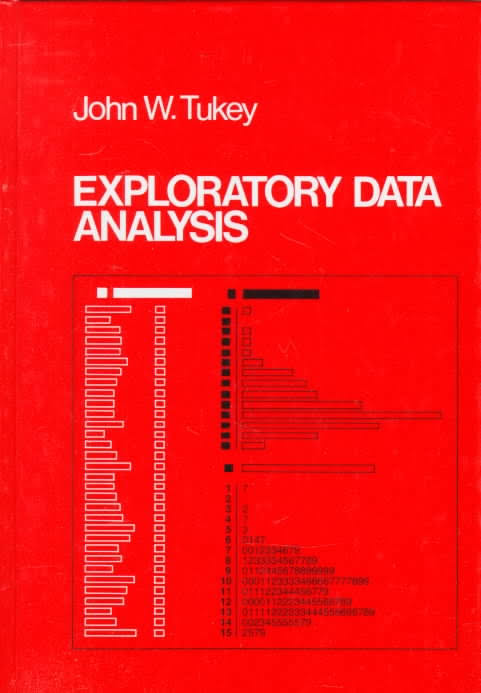
\includegraphics[width=0.4\linewidth]{figures/introduction/tukeyeda}

This book is based on an important principle:

\textbf{It is important to understand what you CAN DO before you learn to measure how WELL you seem to have DONE it.}

Learning first what you can do will help you to work more easily and effectively.

This book is about exploratory data analysis, about looking at data to see what it seems to say. It concentrates on simple arithmetic and easy-to-draw pictures. It regards whatever appearances we have recognized as partial descriptions, and tries to look beneath them for new insights. Its concern is with appearance, not with confirmation.

\hypertarget{examples-not-case-histories}{%
\subsection{Examples, NOT case histories}\label{examples-not-case-histories}}

The book does not exist to make the case that exploratory data analysis is useful. Rather it exists to expose its readers and users to a considerable variety of techniques for looking for effectively at one's data. The examples are not intended to be complete case histories. Rather they show isolated techniques in action on real data. The emphasis is on general techniques, rather than specific problems.

A basic problem about any body of data is to make it more easily and effectively handleable by minds -- our minds, her mind, his mind. To this general end:

\begin{itemize}
\tightlist
\item
  anything that makes a simpler description possible makes the description more easily handleable.
\item
  anything that looks below the previously described surface makes the description more effective.
  So we shall always be glad (a) to simplify description and (b) to describe one layer deeper.
\end{itemize}

In particular

\begin{itemize}
\tightlist
\item
  to be able to say that we looked one layer deeper, and found nothing, is a definite step forward -- though not as far as to be able to say that we looked deeper and found thus-and-such.
\item
  to be able to say that ``if we change our point of view in the following way \ldots{} things are simpler'' is always a gain -- though not quite as much as to be able to say ``if we don't bother to change our point of view (some other) things are equally simple''.
\end{itemize}

Thus, for example, we regard learning that log pressure is almost a straight line in the negative reciprocal of absolute temperature as a real gain, as compared to saying that pressure increases with temperature at an evergrowing rate. Equally, we regard being able to say that a batch of values is roughly symmetrically distributed on a log scale as much better than to say that the raw values have a very skew distribution.

In rating ease of description, after almost any reasonable change of point of view, as very important, we are essentially asserting a belief in quantitative knowledge -- a belief that most of the key questions in our work sooner or later demand answers to ``by how much?'' rather than merely to ``in which direction?''

Consistent with this view, we believe, is a clear demand that pictures based on exploration of data should force their messages upon us. Picture that emphasize what we already know -- ``security blankets'' to reassure us -- are frequently not worth the space they take. Pictures that have to be gone over with a reading glass to see the main point are wasteful of time and inadequate of effect. \textbf{The greatest value of a picture} is when it forces us to notice \textbf{what we never expected to see}.

We shall not try to say why specific techniques are the ones to use. Besides pressures of space and time, there are specific reasons for this. Many of the techniques are less than ten years old in their present form -- some will improve noticeably. And where a technique is very good, it is not at all certain that we yet know why it is.

We have tried to use consistent techniques wherever this seemed reasonable, and have not worried where it didn't. Apparent consistency speeds learning and remembering, but ought not be allowed to outweigh noticeable differences in performance.

In summary, then we:

\begin{itemize}
\tightlist
\item
  leave most interpretations off results to those who are experts in the subject-matter field involved.
\item
  present techniques, not case histories.
\item
  regard simple descriptions as good in themselves.
\item
  feel free to ask for changes in point of view in order to gain such simplicity.
\item
  demand impact from our pictures.
\item
  regard every description (always incomplete!) as something to be lifted off and looked under (mainly by using residuals).
\item
  regard consistency from one technique to another as desirable, not essential.
\end{itemize}

\hypertarget{introduction}{%
\chapter{Introduction}\label{introduction}}

\hypertarget{what-is-data-analysis}{%
\section{What is data analysis?}\label{what-is-data-analysis}}

This is a course in ``data analysis''. Although you have heard this expression many times, you probably don't have a clear idea of what it means. Here is a description of data analysis written by Paul Velleman and David Hoaglin in their article ``Data Analysis'', in \emph{Perspectives on Contemporary Statistics}.

``As the link between statistics and diverse fields of application, data analysis confronts the challenge of turning data into useful knowledge. Data analysis combines an attitude and a process, supported by well-chosen techniques. The attitude distills the scientist's curiosity about regularity, pattern, and exception. The process iteratively peels off patterns so that we can look beneath them for more subtle (and often more interesting) patterns. The techniques make few assumptions about the data and deliberately accommodate the unexpected.''

Essentially exploratory data analysis (abbreviated as EDA) can be viewed as numerical detective work. We are confronted with one or more batches of data and we are trying to uncover patterns in the numbers. Data analysis can be thought of as detective work since it has similarities to the work of a detective, such as the famous Sherlock Holmes, who uncovers a mystery (like the identity of a murderer) from the different evidence that he collects. Our objective in data analysis is to summarize the general structure in the numbers. By doing this, we can describe in a relatively simple way of what the data is telling us.

\hypertarget{what-is-data-and-where-do-we-find-it}{%
\section{What is data and where do we find it?}\label{what-is-data-and-where-do-we-find-it}}

Data are simply numbers with a particular context. For example, the number 610 is data when you are told that 610 represents the number of people who immigrated to the United States from Austria in 1998. Data doesn't need to be a random sample from some hypothetical population. It is simply numbers that we care about and wish to organize and summarize in some effective way.

In this class, you will need to find your own datasets. Where do you find data? Actually, data is present everywhere -- in newspapers, the Internet, and in textbooks. One convenient source of a wide variety of data is the well-known almanac or book-of-facts. (I will be using the 2010 New York Times Almanac which is typical of a world almanac that is available for sale.) Many types of almanacs are available at the library. I recommend purchasing one of the inexpensive paperback almanacs sold at a bookstore. It will be convenient to access an assortment of datasets if you have an almanac readily available.

\hypertarget{meet-our-first-data}{%
\section{Meet our first data}\label{meet-our-first-data}}

Here is a good time to introduce you to our first dataset. Browsing through my almanac, there is a section on immigration in the United States. In this section, the following table is displayed on page 310 that shows the estimated number of U. S. immigrants in 2008 from various countries. The table gives the name of each country, the region of the world in which the country belongs, and the 2008 immigration count from that country. This data is contained in the dataset \texttt{immigrants} in the \texttt{LearnEDA} package. I have listed the first few rows of this data table.

\begin{Shaded}
\begin{Highlighting}[]
\FunctionTok{library}\NormalTok{(LearnEDAfunctions)}
\FunctionTok{head}\NormalTok{(immigrants)}
\end{Highlighting}
\end{Shaded}

\begin{verbatim}
##          Country Region Count.1998 Count.2008
## 1        Austria Europe        610       1505
## 2        Belgium Europe        557        829
## 3 Czechoslovakia Europe        931       1650
## 4        Denmark Europe        447        551
## 5         France Europe       2961       5246
## 6        Germany Europe       6923       8456
\end{verbatim}

Obviously, it is hard to understand general patterns in these immigration numbers by just looking at the table. We are interested in using graphs and summaries to better understand the general structure in these data.

It is usually helpful to list some general questions that we have about these data. Here are a few questions that quickly come to mind:

\begin{itemize}
\tightlist
\item
  What countries have contributed the most immigrants to the United States?
\item
  What is a typical number of immigrants from a country?
\item
  Are Asian countries contributing more or less immigrants than countries from Europe?
\item
  The magazine \emph{Time} had an issue that focused on the U.S./Mexico border. Are we getting an unusually large number of immigrants from Mexico?
\item
  Which countries are contributing a large number of immigrants relative to their population size?
\end{itemize}

We probably won't answer all of these questions in our preliminary data analysis, but it is always important to think of things that you wish to learn from your data.

\hypertarget{how-does-exploratory-data-analysis-eda-differ-from-confirmatory-data-analysis-cda}{%
\section{How does exploratory data analysis (EDA) differ from confirmatory data analysis (CDA)?}\label{how-does-exploratory-data-analysis-eda-differ-from-confirmatory-data-analysis-cda}}

So we can think of exploratory data analysis (EDA) simply as looking for patterns (and deviations from these patterns) in data. This type of data analysis is fundamentally different from the way that most of us learned statistics. Let's illustrate the typical way we learned to analyze a single batch of data.

In this approach, we assume that the data represent a random sample drawn from a hypothetical normally distributed population. With this assumption, a ``best'' guess at the average of the population is the mean. We consider several inferential questions. We construct an interval that we are confident contains the population mean, and we make decisions about the value of the population mean by one or more hypothesis tests. This methodology, based on the t distribution, is well known and available using any statistical software package.

This approach is called confirmatory data analysis or CDA. We analyze data by the use of probability models. We write down a family of probability models that could have generated the observed data, and we learn about the data by estimating the unknown parameters of these models.

\hypertarget{how-is-eda-different-from-cda}{%
\section{How is EDA different from CDA?}\label{how-is-eda-different-from-cda}}

First, in EDA we make no assumptions about an underlying population. We don't assume that the data represent independent observations or that the data come from a population with a prescribed shape. The data are simply viewed as numbers that we wish to explore.

Second, the goals of EDA are different from that of CDA. The goal of CDA is to learn about the underlying population -- statistical inference is the goal of CDA. In contrast, there are no inferential goals in EDA. We are focusing our analysis on the data at hand, instead of worrying about characteristics of a hypothetical population.

I don't want to give you the impression that EDA is in some sense better than CDA. Rather, data analysis typically consists of both EDA and CDA. In a typical data analysis, we will use EDA methods to discover basic patterns or structure in the data. Then we may later use inferential methods to make statements about underlying populations.

\hypertarget{john-tukeys-contribution}{%
\section{John Tukey's contribution}\label{john-tukeys-contribution}}

Exploratory data analysis will always be associated with John Tukey, who was one of the greatest statisticians in history. It would be wrong to say that Tukey invented EDA. Rather, Tukey was the first to organize a collection of methods and associated philosophy into what we call EDA. There is an orange text called \emph{EDA} that describes this work. Some of the data analysis methods Tukey used were novel and he gave them interesting names, like stem-and-leaf, boxplot, resistant smooth, and rootogram. It is natural for students to focus on the particular data analysis methods developed by Tukey. But Tukey's legacy in this area was not the EDA methods but rather the particular data analysis philosophy that underlies the development of these methods.

\hypertarget{four-principles-of-eda-the-four-rs}{%
\section{Four principles of EDA (the four R's)\}}\label{four-principles-of-eda-the-four-rs}}

Although we will discuss a variety of methods useful for exploring data, they all share different characteristics that underlie the philosophy of EDA. We call these principles the four R's since each principle starts with the letter r.

\begin{itemize}
\item
  \textbf{Revelation:} In EDA, there is an emphasis on using graphs to find patterns or displaying fits. Effective displays of data can communicate information in way that is not possible by the use of numbers. A good rule of thumb is to always graph your data before commuting any summary statistic. There will be a lot of graphing in this course, and we'll discuss guidelines for constructing effective graphs.
\item
  \textbf{Resistance:} In EDA, we wish to describe the general pattern in the majority of the data. In this detective work, we don't want our search to be unusually affected by a few unusual observations. So it is important that our exploratory method is resistant or insensitive to outliers. When we look at a single batch of numbers, we'll see that the median or middle value (when the data are arranged in ascending order) is an example of a resistant measure. The mean or arithmetic average is nonresistant since it can be distorted by one or more extreme values.
\item
  \textbf{Reexpression:} We will see that the natural scale that the data is presented is not always the best scale for displaying or summarizing the data. In many situations, we wish to reexpress the data to a new scale by taking a square root or a logarithm. In this class, we will talk about a useful class of reexpressions, called the power family, and give guidance on the ``best'' choice of power reexpression to simplify the data analysis.
\item
  \textbf{Residual:} In a typical data analysis, we will find a general pattern, which we call the FIT. The description of the FIT may be very informative. But in EDA we wish to look for deviations in the data from the general pattern in the FIT. We look at the residuals, which are defined as the difference between the data and the FIT.
  \[
  RESIDUAL = DATA - FIT
  \]
  In many situations, we will see that a careful investigation of the residuals may be more interesting than the fit.
\end{itemize}

\hypertarget{an-exploratory-look-at-our-data}{%
\section{An exploratory look at our data}\label{an-exploratory-look-at-our-data}}

Let's illustrate a few of the EDA principles in an analysis of our immigration data. We start with a graph of the immigration counts. A simple graph is a stripchart that represents each value by a dot over the appropriate place on a number line. The points have been randomly jittered in the vertical direction so one can see overlapping points.

\begin{Shaded}
\begin{Highlighting}[]
\FunctionTok{library}\NormalTok{(tidyverse)}
\FunctionTok{ggplot}\NormalTok{(immigrants,}
       \FunctionTok{aes}\NormalTok{(}\AttributeTok{x =}\NormalTok{ Count}\FloatTok{.2008}\NormalTok{, }\AttributeTok{y =} \DecValTok{1}\NormalTok{)) }\SpecialCharTok{+}
     \FunctionTok{geom\_jitter}\NormalTok{() }\SpecialCharTok{+} \FunctionTok{ylim}\NormalTok{(}\DecValTok{0}\NormalTok{, }\DecValTok{2}\NormalTok{) }\SpecialCharTok{+}
     \FunctionTok{theme}\NormalTok{(}\AttributeTok{axis.title.y=}\FunctionTok{element\_blank}\NormalTok{(),}
     \AttributeTok{axis.text.y=}\FunctionTok{element\_blank}\NormalTok{(),}
     \AttributeTok{axis.ticks.y=}\FunctionTok{element\_blank}\NormalTok{())}
\end{Highlighting}
\end{Shaded}

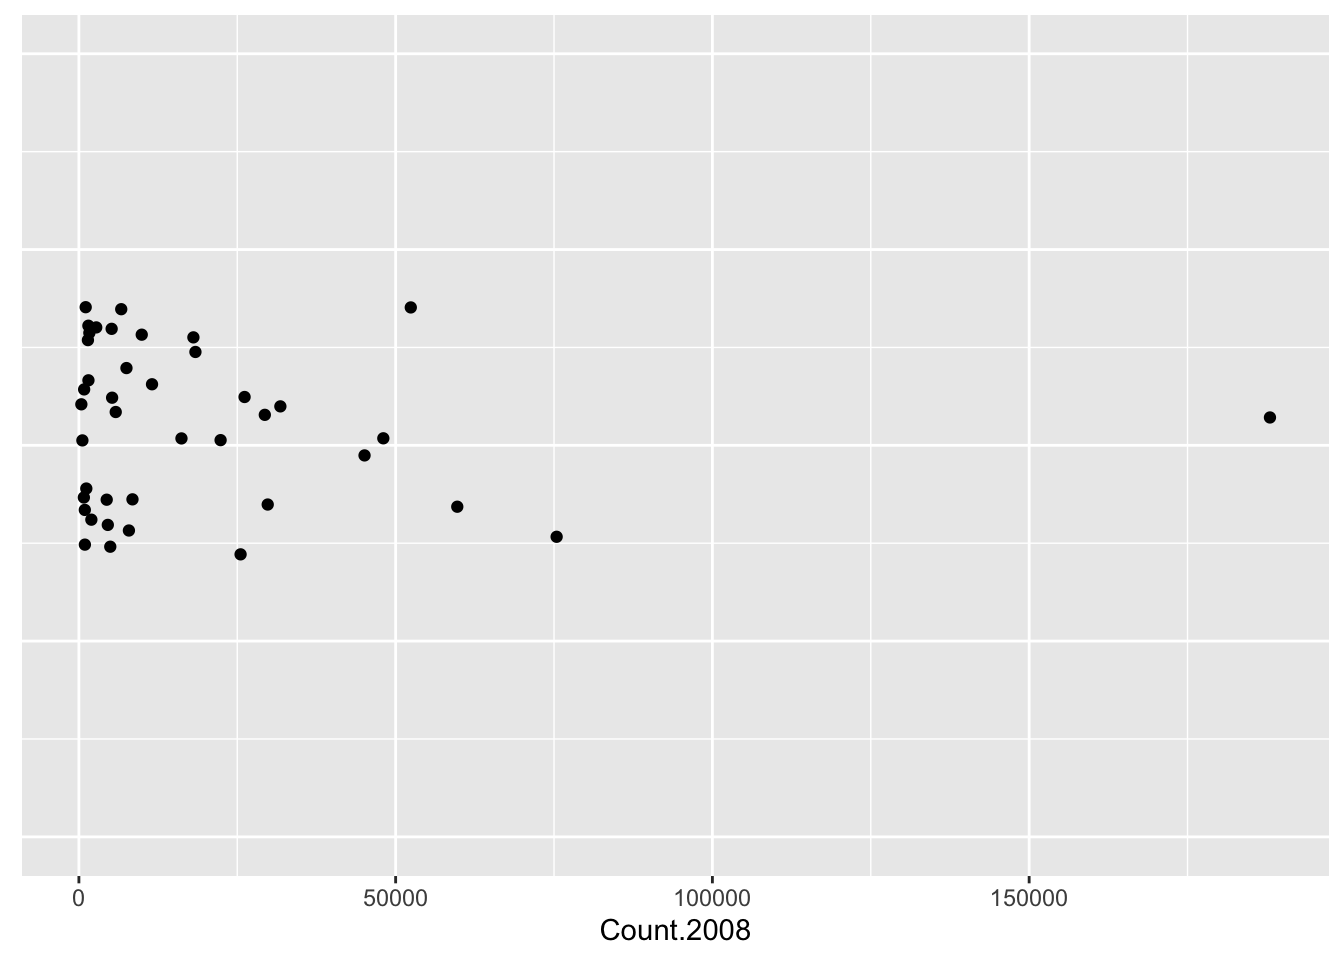
\includegraphics{Course-in-Exploratory-Data-Analysis_files/figure-latex/unnamed-chunk-3-1.pdf}

Looking at this stripchart, we see that most of the immigration counts are clustered between 0 and 30,000 with only six countries appear to have large counts.

This is really not a very useful graphical display since most of the data is bunched up towards the value zero. In other words, this data is strongly right-skewed. Due to this right-skewness, all we have learned is that there are a few countries with large numbers of immigrants and Mexico, with 188,015 immigrants, stands out.

What we see in this stripchart is that the original data (counts of immigrants) is not the best scale for viewing in a graph. We can improve the presentation of these data by reexpressing the counts by taking logs. That is, we reexpress Austria's count 1505 to log(1505) = 2.79, reexpress Belgium's count 557 to log(557) = 3.18, and so on for all of the immigrant counts. (By the way, when we take logs in this class, they will all be log base 10.)

\begin{Shaded}
\begin{Highlighting}[]
\NormalTok{immigrants }\OtherTok{\textless{}{-}} \FunctionTok{mutate}\NormalTok{(immigrants,}
                     \AttributeTok{log.Count =} \FunctionTok{log10}\NormalTok{(Count}\FloatTok{.2008}\NormalTok{))}
\end{Highlighting}
\end{Shaded}

Here is a stripchart of the logarithms of the immigrant counts:

\begin{Shaded}
\begin{Highlighting}[]
\FunctionTok{ggplot}\NormalTok{(immigrants,}
       \FunctionTok{aes}\NormalTok{(}\AttributeTok{x =}\NormalTok{ log.Count, }\AttributeTok{y =} \DecValTok{0}\NormalTok{)) }\SpecialCharTok{+}
     \FunctionTok{geom\_jitter}\NormalTok{() }\SpecialCharTok{+} \FunctionTok{ylim}\NormalTok{(}\SpecialCharTok{{-}}\DecValTok{1}\NormalTok{, }\DecValTok{1}\NormalTok{) }\SpecialCharTok{+}
     \FunctionTok{theme}\NormalTok{(}\AttributeTok{axis.title.y=}\FunctionTok{element\_blank}\NormalTok{(),}
     \AttributeTok{axis.text.y=}\FunctionTok{element\_blank}\NormalTok{(),}
     \AttributeTok{axis.ticks.y=}\FunctionTok{element\_blank}\NormalTok{())}
\end{Highlighting}
\end{Shaded}

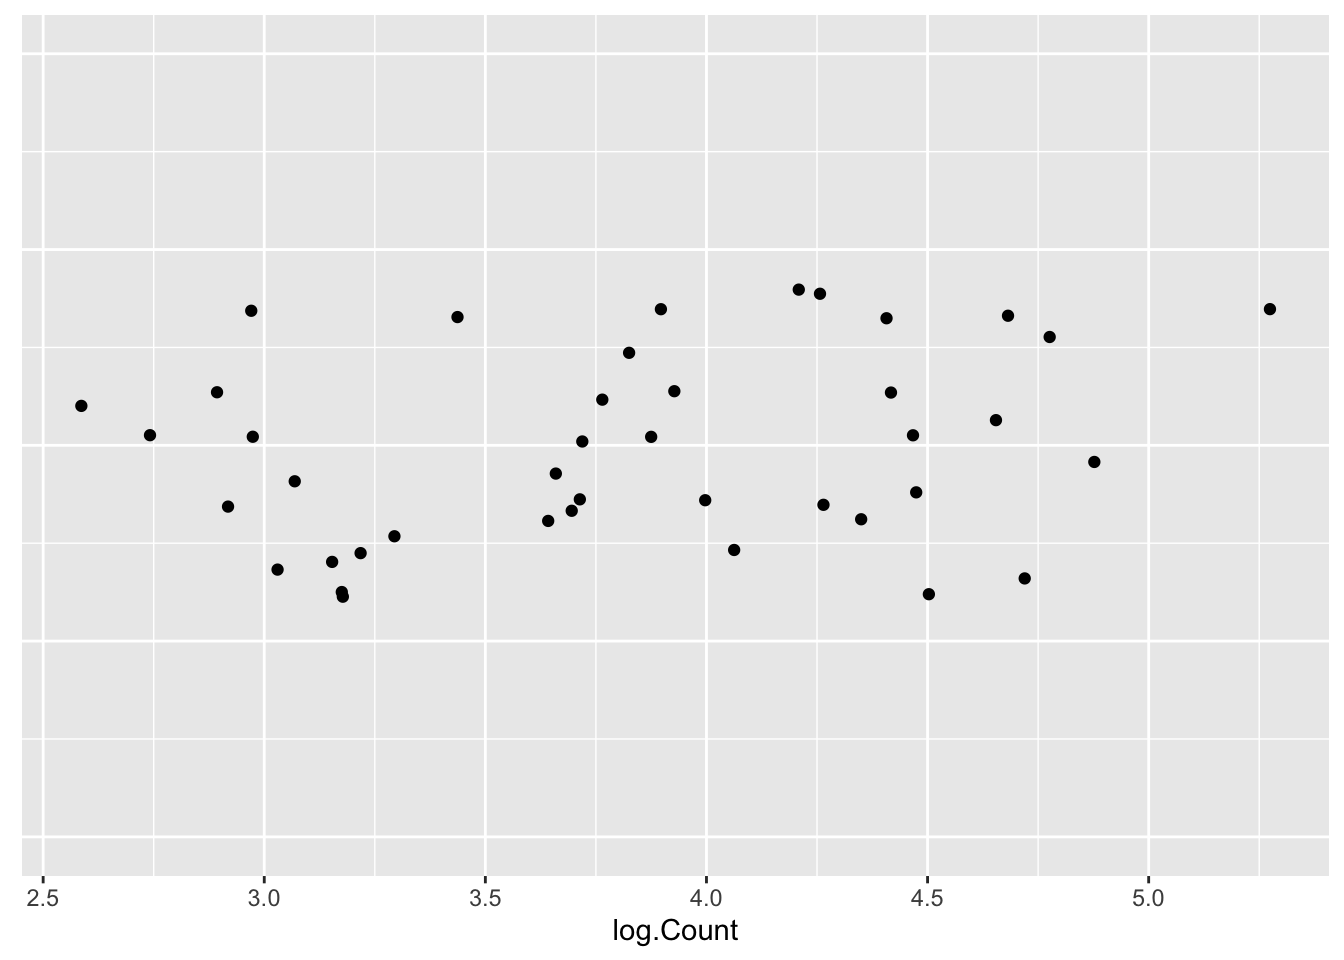
\includegraphics{Course-in-Exploratory-Data-Analysis_files/figure-latex/unnamed-chunk-5-1.pdf}

This is a much better graphical display for viewing these data. The log counts are evenly spread out between 2.50 and 5.20 and one can see more interesting structure in the data. In particular, we see a clump of countries with log immigration counts around 3, and a second concentration of log counts around 4. A typical log immigration count can be seen to be about 3.75. We still see Mexico's large log count of 5.27; but now we also see a small log count at 2.58 that corresponds to Norway.

We can summarize these data by the typical value of 3.75 -- this is our FIT to these data. We can compute residuals by subtracting the FIT from each log count:
\[
RESIDUAL = \log COUNT - FIT
\]
\[
= \log COUNT - 3.75
\]

\begin{Shaded}
\begin{Highlighting}[]
\NormalTok{immigrants }\OtherTok{\textless{}{-}} \FunctionTok{mutate}\NormalTok{(immigrants,}
              \AttributeTok{Residual =}\NormalTok{ log.Count }\SpecialCharTok{{-}} \FloatTok{3.75}\NormalTok{)}
\end{Highlighting}
\end{Shaded}

The stripchart below graphs the residuals of the data:

\begin{Shaded}
\begin{Highlighting}[]
\FunctionTok{ggplot}\NormalTok{(immigrants,}
       \FunctionTok{aes}\NormalTok{(}\AttributeTok{x =}\NormalTok{ Residual, }\AttributeTok{y =} \DecValTok{0}\NormalTok{)) }\SpecialCharTok{+}
     \FunctionTok{geom\_jitter}\NormalTok{() }\SpecialCharTok{+} \FunctionTok{ylim}\NormalTok{(}\SpecialCharTok{{-}}\DecValTok{1}\NormalTok{, }\DecValTok{1}\NormalTok{) }\SpecialCharTok{+}
     \FunctionTok{theme}\NormalTok{(}\AttributeTok{axis.title.y=}\FunctionTok{element\_blank}\NormalTok{(),}
     \AttributeTok{axis.text.y=}\FunctionTok{element\_blank}\NormalTok{(),}
     \AttributeTok{axis.ticks.y=}\FunctionTok{element\_blank}\NormalTok{())}
\end{Highlighting}
\end{Shaded}

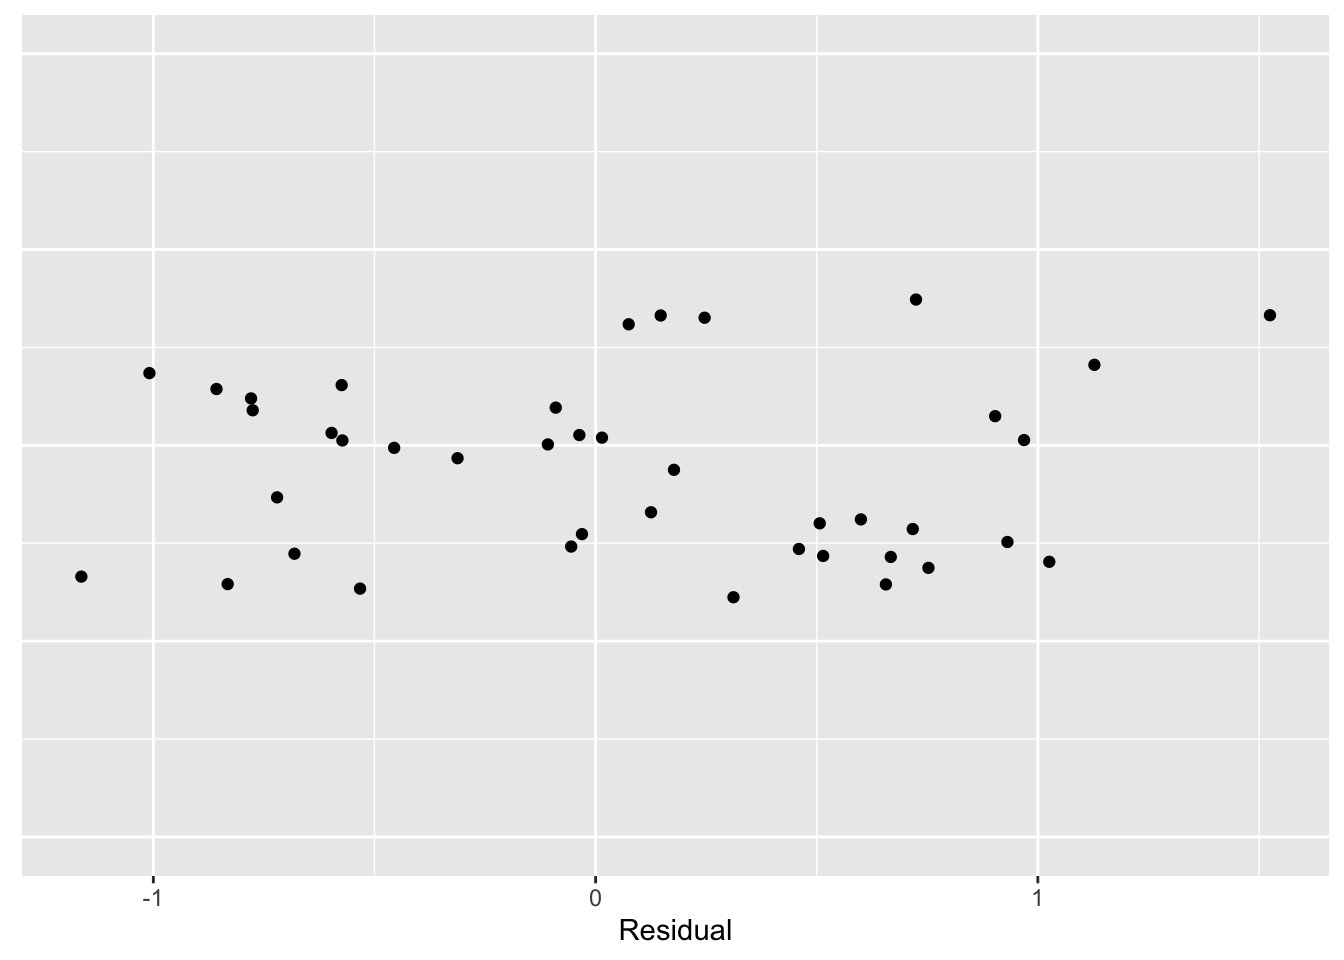
\includegraphics{Course-in-Exploratory-Data-Analysis_files/figure-latex/unnamed-chunk-7-1.pdf}

Now we can look at these data in more detail. We see that, on the log count scale, two countries have immigration counts that are 1 smaller than the average; also there is one country (Mexico) that is approximately 1.5 larger than the average. This residual graph tells how close the log counts are to the average of 3.75.

This example illustrates a few of the EDA principles that we'll be using throughout the course.

\begin{itemize}
\tightlist
\item
  It illustrates the use of graphical displays to see basic patterns in data.
\item
  It shows that the scale of the original data may not be the best scale for viewing data and one can reexpress the data by a suitable transformation (here logs) to improve the presentation of the data.
\item
  One can easily summarize the reexpressed data by a ``typical'' value, and residuals can be computed that show the deviations of the data from this typical value.
\end{itemize}

\textbf{What have we learned?}

Let's return to our questions about these data to see what we have learned in this brief data analysis:

\begin{itemize}
\tightlist
\item
  What countries have contributed the most immigrants to the United States?
\end{itemize}

ANSWER: Mexico is by far the leader in supplying immigrants to the U.S.

\begin{itemize}
\tightlist
\item
  What is a typical number of immigrants from a country?
\end{itemize}

ANSWER: On the log scale, a typical immigrant count is 3.75.

\begin{itemize}
\tightlist
\item
  Are Asian countries contributing more or less immigrants than countries from Europe?
\end{itemize}

ANSWER: We didn't address this question in our brief analysis, but we'll soon talk about how we can compare batches of data.

\begin{itemize}
\tightlist
\item
  The magazine \emph{Time} had an issue that focused on the U.S./Mexico border. Are we getting an unusually large number of immigrants from Mexico?
\end{itemize}

ANSWER: Yes -- this analysis confirms that Mexico is supplying many immigrants.

\begin{itemize}
\tightlist
\item
  Which countries are contributing a large number of immigrants relative to their population size?
\end{itemize}

ANSWER: In order to answer this question, we would need to collect the populations of the countries in the table. This would be an interesting study.

\hypertarget{working-with-a-single-batch-displays}{%
\chapter{Working with a Single Batch -- Displays}\label{working-with-a-single-batch-displays}}

\hypertarget{meet-the-data}{%
\section{Meet the Data}\label{meet-the-data}}

\textbf{Data: ACT Average Composite Scores by State, 2006-2007}

Source: ACT, Inc.~from the World Almanac and Book of Facts 2008.

One of the most important standardized tests given in the United States is the ACT exam. This test is used by many universities in deciding acceptance of prospective freshmen. The table below shows the ACT average composite score for 26 states. Here we are focusing only on the states where at least half of the high school graduates took this exam.

\begin{verbatim}
   State ACT State  ACT 
         Avg       Avg
-------------------------------------
    AL  20.3  MO    21.6
    AR  20.5  MT    21.9
    CO  20.4  NE    22.1
    FL  19.9    NM  20.2
    ID  21.4    ND  21.6
    IL  20.5    OH  21.6
    IA  22.3    OK  20.7
    KS  21.9    SD  21.9
    KY  20.7    TN  20.7
    LA  20.1    UT  21.7
    MI  21.5    WV  20.6
    MN  22.5    WI  22.3
    MS  18.9    WY  21.5
\end{verbatim}

\hypertarget{the-basic-stemplot}{%
\section{The Basic Stemplot}\label{the-basic-stemplot}}

Our first task in working with this batch of data is to organize it in some way so that we can see the distribution of ACT averages. A simple, yet effective display of a small amount of data is a stem and leaf diagram, or stemplot for short.

Here are the steps for drawing a stemplot.

\begin{itemize}
\tightlist
\item
  First, divide each data value into a stem and a leaf.
\end{itemize}

Here it is convenient to divide a ACT average, such as Alabama's
20.3 value into a

\begin{verbatim}
stem of 20 and a leaf of 3.
\end{verbatim}

(Note: here we are dividing at the decimal point, but this won't usually be the case.)

\begin{itemize}
\tightlist
\item
  Next, we write down all of the possible stems.
\end{itemize}

\begin{verbatim}
18
19
20
21
22
\end{verbatim}

\begin{itemize}
\tightlist
\item
  We record values by placing the leaf for each data item on its corresponding stem.
\end{itemize}

So Alabama's 20.3 value is recorded as

\begin{verbatim}
18
19
20 3
21
22
\end{verbatim}

We next record Arizona's 20.5 value as

\begin{verbatim}
18
19
20 35
21
22
\end{verbatim}

\begin{itemize}
\tightlist
\item
  Continuing in this fashion, we record all 26 ACT averages.
\end{itemize}

\begin{verbatim}
 1 | 2: represents 1.2
 leaf unit: 0.1
           
     18 9
     19 9
     20 1234556777
     21 4556667999
     22 1335
\end{verbatim}

Note that we have indicated the unit for each leaf. This is important since we have thrown away the decimal point in creating the stemplot. If we look at the stemplot, the first value is

\begin{verbatim}
18 9
\end{verbatim}

which we interpret as 189 (.1) = 18.9 since the unit is .1.

The stemplot is a quick way of grouping the averages. It resembles the better-known graphical display, the histogram. If you were to construct a histogram using the intervals 18-19, 19-20, and so on, you would obtain the following picture that resembles the stemplot above.

\begin{Shaded}
\begin{Highlighting}[]
\FunctionTok{library}\NormalTok{(LearnEDAfunctions)}
\FunctionTok{library}\NormalTok{(ggplot2)}
\FunctionTok{ggplot}\NormalTok{(act.scores.}\FloatTok{06.07}\NormalTok{, }\FunctionTok{aes}\NormalTok{(ACT)) }\SpecialCharTok{+}
  \FunctionTok{geom\_histogram}\NormalTok{(}\AttributeTok{breaks =} \DecValTok{17}\SpecialCharTok{:}\DecValTok{24}\NormalTok{,}
                 \AttributeTok{color=}\StringTok{"black"}\NormalTok{, }\AttributeTok{fill=}\StringTok{"white"}\NormalTok{)}
\end{Highlighting}
\end{Shaded}

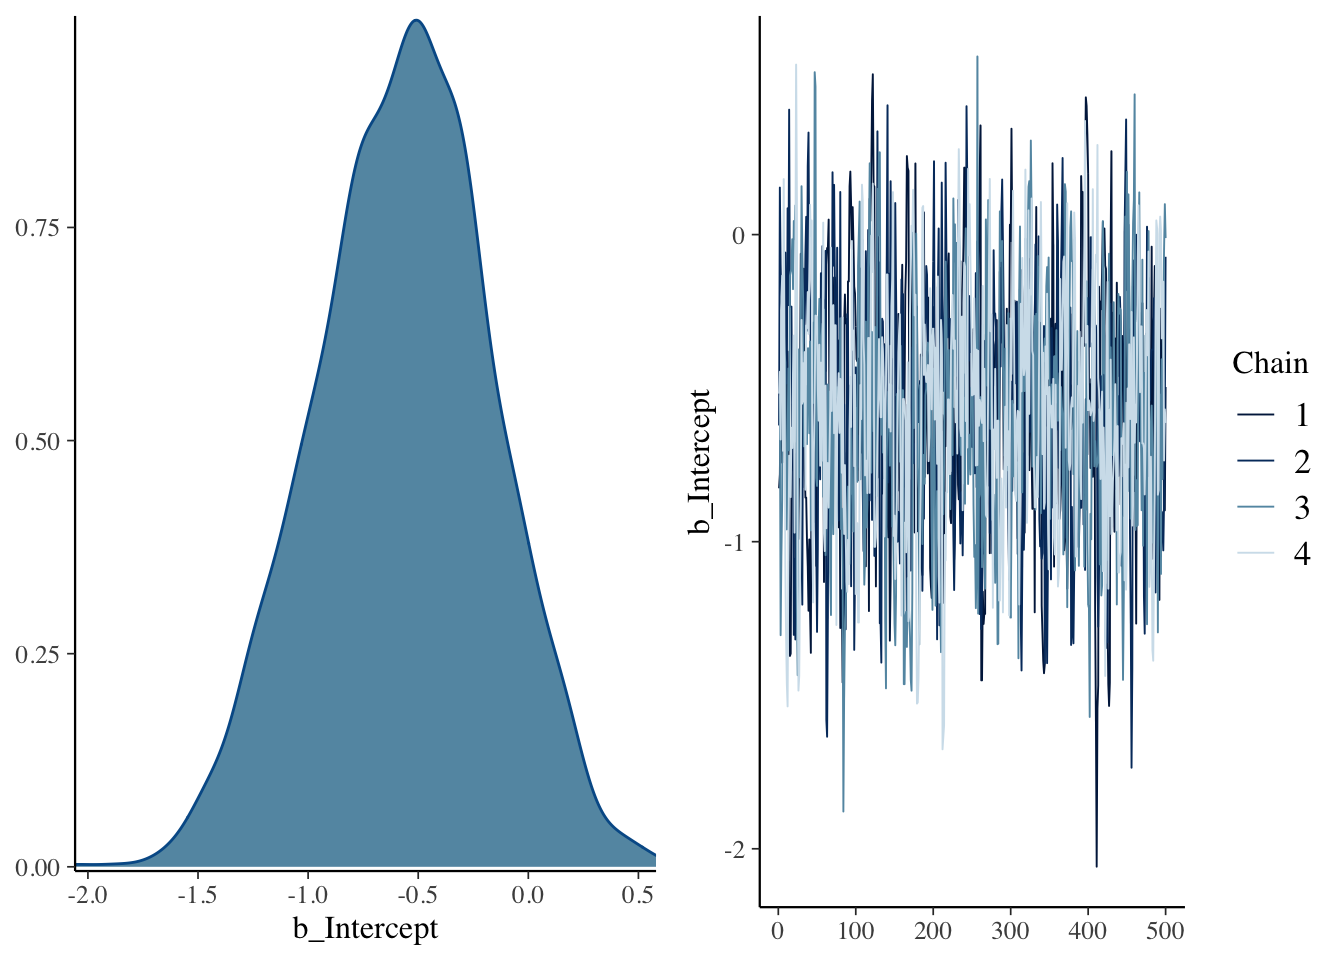
\includegraphics{Course-in-Exploratory-Data-Analysis_files/figure-latex/unnamed-chunk-8-1.pdf}

However, the stemplot has one strong advantage over a histogram. You can actually see the data values that fall in each interval. For example, we see that the last line contains the four largest ACT averages 22.1, 22.3, 22.3, 22.5 corresponding respectively to the states Nebraska, Iowa, Wisconsin, and Minnesota . In a histogram, we would lose this information about individual states when we group the data items in the individual classes.

\hypertarget{looking-at-a-data-distribution}{%
\section{Looking at a Data Distribution}\label{looking-at-a-data-distribution}}

What do we look for when we display data using a graph like a stemplot?

\begin{enumerate}
\def\labelenumi{\arabic{enumi}.}
\tightlist
\item
  First, we look at the \textbf{general shape} of the data. (The stemplot of the ACT averages has been redrawn below.)
\end{enumerate}

\begin{verbatim}
     18 9
     19 9
     20 1234556777
     21 4556667999
     22 1335
\end{verbatim}

Generally, we distinguish between three basic data shapes -- symmetric, skewed right and skewed left.

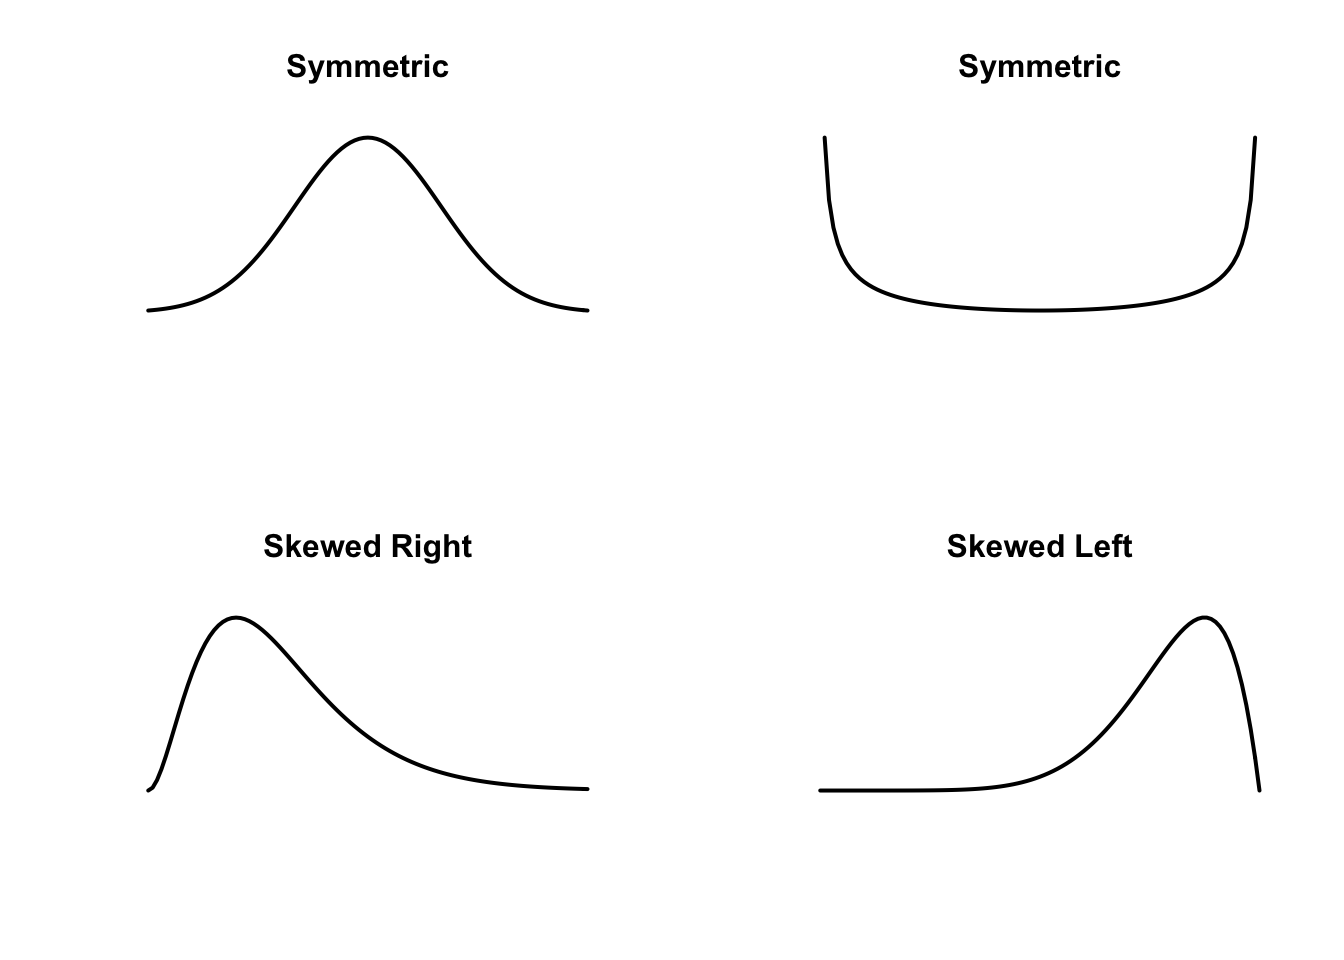
\includegraphics{Course-in-Exploratory-Data-Analysis_files/figure-latex/unnamed-chunk-9-1.pdf}

\textbf{Symmetric} is when the majority of the data is in the middle and the values drop off at the same rate at the low end and the right end. You can imagine dividing the data into two halves, where the left half is approximately a mirror image of the right half.

\textbf{Skewed right} is where the data values at the high end decrease at a much slower rate than the values at the low end. Conversely, \textbf{skewed left} is where the data values at the low end decrease at a slower rate than the values at the high end.

One can represent these three shapes by means of smoothed curves.

What can we say about our dataset? It is hard to tell (we will try alternative displays of these data to get a better look), but to me it appears somewhat skewed left. Most of the ACT averages fall in the 20-21 range and the values at the low end decrease at a slower rate than averages at the high end.

\begin{enumerate}
\def\labelenumi{\arabic{enumi}.}
\setcounter{enumi}{1}
\item
  After we think about shape, we want to talk about a \textbf{typical} or average value\}. We will later describe different types of ``averages'', but we notice the large number of ACT averages in the 21 line, so 21.something would be a typical value.
\item
  Next, we describe the \textbf{spread or variation} in the data values. We see that most of the ACT averages fall between 20 and 22.1, with only a couple of states with averages below 20.
\item
  Last, we discuss any \textbf{unusual data values} or any \textbf{distinctive features} of this distribution. Here we might talk about
\end{enumerate}

\begin{itemize}
\tightlist
\item
  unusually high or low values
\item
  any gaps in the data
\item
  the presence of several clusters of observations
\item
  granularity in the data -- possibly all of the data values end with an even last digit
\end{itemize}

Here we don't see anything particularly unusual. The two low ACT averages were already mentioned. Part of the reason why we don't see more is that we could improve our graphical display. This motivates talking about variations of the basic stemplot.

\hypertarget{stemplot-variations-breaking-the-stem-at-different-locations}{%
\section{Stemplot variations -- breaking the stem at different locations}\label{stemplot-variations-breaking-the-stem-at-different-locations}}

In our stemplot, we formed the stem and leaf by dividing at the decimal point. But other break points are possible.

To illustrate, we could break Alabama's 20.3 ACT average between the units and tens place:

\begin{verbatim}
2  |  03
\end{verbatim}

Then we would jot down Alabama's value on the stemplot

\begin{verbatim}
     1 
     2 0
\end{verbatim}

Note that we use the one-digit leaf 0 -- we drop off the last digit 2 in 03. (We typically draw stemplots using single digits for leaves.)

By the way, it is better to drop and not round. Rounding takes more time than dropping. Also it is easier to retrieve the original data from the stemplot when you drop digits.

With this breakpoint, we get the following display for the 26 ACT averages:

\begin{verbatim}
1 | 2: represents 12
 leaf unit: 1
      n: 26
   1  89
   2  000000000011111111112222
\end{verbatim}

This is not a very effective display, since all the data is bunched up on only two lines.

Another possibility is to break an ACT average between the tenth and hundredth places. If we write Alabama's value 20.3 as 20.30, we break as follows:

\begin{verbatim}
  203 | 0
\end{verbatim}

Here there are quite a few possible stems -- from 189 to 225. We could write down the corresponding display, but it would consist of 37 lines. Given that we have only 26 data values to show, it should be clear that the display would be stretched out too much.

\hypertarget{stemplot-variations-2-5-and-10-leaves-per-stem}{%
\section{Stemplot variations -- 2, 5, and 10 leaves per stem}\label{stemplot-variations-2-5-and-10-leaves-per-stem}}

There is another choice in constructing a stemplot -- the number of possible leaves on each stem. In our basic display (shown again)

\begin{verbatim}
     18 79
     19 69
     20 123345556777
     21 024455566667788999
     22 00011233355899
     23 125
\end{verbatim}

there are 10 possible leaves on each line (that is, 0, 1, 2, \ldots, 9), and so we call this display a stemplot with 10 leaves per stem.

One way of stretching out this display is to divide the ten possible leaves into a small group (0 through 4) and a large group (5 through 9). To draw this stemplot, we write down each stem twice

\begin{verbatim}
     18*
     18.
     19*
     19.
     20*
     20.
     21*
     21.
     22*
     22.
     23*
     23.
\end{verbatim}

(the * indicates the first line and . the second) and then record the leaves

\begin{verbatim}
1 | 2: represents 1.2
 leaf unit: 0.1
        n: 26
    18. 9
    19* 
    19. 9
    20* 1234
    20. 556777
    21* 4
    21. 556667999
    22* 133
    22. 5
\end{verbatim}

We call this display a stemplot with 5 leaves per stem. I think this is a better graph than the 10-lines-per-stem since we see more structure. Now we see

\begin{itemize}
\tightlist
\item
  two clusters of observations -- one cluster in the 20* line and a second in the 21. line. It might be reasonable to say that there are two modes or humps in the data.
\item
  the 18.7 and 18.9 values appears to be somewhat low, since there is a gap between these ACT averages and the next largest
\end{itemize}

Another possible stemplot is to divide the 10 possible leaves in our basic display into 5 groups. We write the 18 line five times

\begin{verbatim}
  18*
    18t
    18f
    18s
    18.
\end{verbatim}

The 0, 1 leaves are written on the first line (*), the 2, 3 leaves are put on the 2nd (t) line, the 4, 5 leaves on the (f) line, the 6, 7 leaves on the (s) line and the 8, 9 leaves on the (.) line. The use of the t, f, s labels is helpful, since TWO and THREE start with t, FOUR and FIVE start with f, and SIX and SEVEN start with s. (I guess this idea wouldn't be helpful in drawing a stemplot with Chinese letters.)

We call this display a stemplot with 2 leaves per stem, since each line has two possible leaves. This stemplot for our data is shown below.

\begin{verbatim}
1 | 2: represents 1.2
 leaf unit: 0.1
            n: 26
   18. | 9
   19* | 
     t | 
     f | 
     s | 
   19. | 9
   20* | 1
     t | 23
     f | 455
     s | 6777
   20. | 
   21* | 
     t | 
     f | 455
     s | 6667
   21. | 999
   22* | 1
     t | 33
     f | 5
\end{verbatim}

Which is a better display, the previous one with 5 leaves per stem, or this one with 2 leaves per stem? This last display looks too spread out to me. You do see the two clusters in this 2-leaves-per-stem stemplot, but there are more gaps introduced since we stretched out the display.

\hypertarget{guidance-in-constructing-a-stemplot}{%
\section{Guidance in Constructing a Stemplot}\label{guidance-in-constructing-a-stemplot}}

In constructing a stemplot, there are two choices to make:

\begin{itemize}
\tightlist
\item
  how to break between the stem and leaf
\item
  how many leaves per stem to use
\end{itemize}

It is best to try a few different stemplots and use the one that you think best represents the data. You will get some experience hand-drawing stemplots -- every time you should try at least two displays. The second display is usually quick to draw once the first display is done.

\hypertarget{making-the-stemplot-resistant}{%
\section{Making the Stemplot Resistant}\label{making-the-stemplot-resistant}}

Let's illustrate constructing stemplots using a second example. In our almanac (page 953), the the weights of the heaviest fish caught are listed for various species. I have jotted down the weights in pounds for the first 25 fish in the table (from Albacore to Summer Flounder):

\begin{verbatim}
88  155  85  21  26  13  10  563  78  31  19  18  21  23  135     
98   35 133  88 113  94   9   36  20  22
\end{verbatim}

To construct a stemplot, we first might trying breaking between the unit and the tens digits. If we do, we will get 56 lines, which won't fit on a single page. The problem is that there is a single large weight 563 (corresponding to a Giant Sea Bass) which is larger than all of the remaining observations. We would like our display to be resistant or not distorted by a single large value. So what we do is to draw a stemplot of the values with the large value listed on a separate line labelled ``HI''.

\begin{verbatim}
      0 9
      1 0389
      2 011236
      3 156
      4 
      5 
      6 
      7 8
      8 588
      9 48
     10 
     11 3
     12 
     13 35
     14 
     15 5

     HI  563,

     Unit = 1 
\end{verbatim}

This graph shows two clusters of weights, one in the 10-20 pound range, and a second in the 80's. This display might spread out the data too much. So, as an alternative, let's try breaking the data between the 10's and 100's places and using two leaves per stem.

\begin{verbatim}
       0* 01111
       0t 222222333
       0f 
       0s 7
       0. 88899
       1* 1
       1t 33
       1f 5

       HI  563,

       Unit = 10 
\end{verbatim}

I like this display better than the previous one. I still see two basic clusters in the datasets separated by a gap. This means that many of the record fish weights are modest size (corresponding to small fish), a second group of weights correspond to moderate-size fish, and we can't ignore the large weight of the Giant Sea Bass.

\hypertarget{a-few-closing-comments}{%
\section{A Few Closing Comments}\label{a-few-closing-comments}}

\begin{itemize}
\item
  Although we have focused our discussion on the stemplot, it is not always the best graphical display. A stemplot is most effective for a dataset with no more than 50 values. If you have a larger dataset, it is likely that you would need too many stemplot lines. For large datasets, it is better to use a histogram.
\item
  It is instructive to experiment with different choices of breakpoint and leaves per stem to find the ``best'' stemplot. But it is handy to have a formula which gives a suggested stemplot for a given dataset.
\end{itemize}

Here is a useful rule-of-thumb. The stemplot should have L lines where

\[
L = [10 \log10(n)],
\]

where \([ \, ]\) stands for the integer part of the argument.

How should we use this formula?

\begin{itemize}
\tightlist
\item
  Find the range R of the data and compute L.
\item
  Divide R by L, and round the answer to 2, 5, or 10.
\item
  This answer gives you the breakpoint and the number of leaves per stem.
\end{itemize}

Let's illustrate this rule for our ACT scores. We have n = 26 scores and LO = 18.7, HI = 23.5.

The range is equal to

\begin{Shaded}
\begin{Highlighting}[]
\NormalTok{(R }\OtherTok{\textless{}{-}} \FloatTok{23.5} \SpecialCharTok{{-}} \FloatTok{18.7}\NormalTok{)}
\end{Highlighting}
\end{Shaded}

\begin{verbatim}
## [1] 4.8
\end{verbatim}

and

\begin{Shaded}
\begin{Highlighting}[]
\NormalTok{(L }\OtherTok{\textless{}{-}} \FunctionTok{floor}\NormalTok{(}\DecValTok{10} \SpecialCharTok{*} \FunctionTok{log10}\NormalTok{(}\DecValTok{26}\NormalTok{)))}
\end{Highlighting}
\end{Shaded}

\begin{verbatim}
## [1] 14
\end{verbatim}

So the ratio of R over L is given by

\begin{Shaded}
\begin{Highlighting}[]
\NormalTok{R }\SpecialCharTok{/}\NormalTok{ L}
\end{Highlighting}
\end{Shaded}

\begin{verbatim}
## [1] 0.3428571
\end{verbatim}

which I round to 0.2 (it is closer to 0.2 than to 0.5) So the distance between the smallest value in two consecutive lines of the stemplot should be 0.2.

This rule tells us to use the display where we break 18.7 at the decimal point, and use two leaves per stem. This is the stemplot that started like

\begin{verbatim}
    18*
    18t
    18f
    18s 7
    18. 9
\end{verbatim}

Actually, we decided that stemplot with 5 leaves per stem seemed better, but at least this rule gives us a stemplot that is close to the best one.

\hypertarget{single-batch-summaries}{%
\chapter{Single Batch: Summaries}\label{single-batch-summaries}}

\hypertarget{meet-the-data-1}{%
\section{Meet the Data}\label{meet-the-data-1}}

\textbf{Data: Percentage change in population 2000-2009 for each state.}

\textbf{Source: The 2010 New York Times Almanac, page 277, and the U.S. Census Bureau website \url{http://www.census.gov}. }

This data (some that is displayed in the following table) shows the change in population (measured in terms of a percentage) for all states in the United States between the years 2000 and 2009 (roughly between the 2000 and 2010 census). This is interesting data, since we are interested in the regions of the U.S. which are growing fast and slow. Specifically, we might want to know

\begin{itemize}
\tightlist
\item
  what is a typical growth rate for a state in the last 9 years?
\item
  are there states whose growths are significantly different from the typical growth rate?
\item
  do the states with large population growths correspond to particular regions of the U.S.?
\end{itemize}

In this topic, we'll discuss simple ways of summarizing a dataset. These summaries and associated displays will help in answering some of these questions.

\begin{Shaded}
\begin{Highlighting}[]
\FunctionTok{library}\NormalTok{(LearnEDAfunctions)}
\FunctionTok{library}\NormalTok{(tidyverse)}
\FunctionTok{select}\NormalTok{(pop.change, State, Pct.change) }\SpecialCharTok{\%\textgreater{}\%} \FunctionTok{head}\NormalTok{()}
\end{Highlighting}
\end{Shaded}

\begin{verbatim}
##        State Pct.change
## 1    Alabama        5.9
## 2     Alaska       11.3
## 3    Arizona       28.6
## 4   Arkansas        8.1
## 5 California        9.1
## 6   Colorado       16.8
\end{verbatim}

We begin by constructing a stemplot of the growth percentages. We break between the ones and tens places and use two leaves per stem. We have one unusual value -- Nevada at the high end that we show on a separate HI line.

\begin{Shaded}
\begin{Highlighting}[]
\NormalTok{aplpack}\SpecialCharTok{::}\FunctionTok{stem.leaf}\NormalTok{(pop.change}\SpecialCharTok{$}\NormalTok{Pct.change, }\AttributeTok{depth=}\ConstantTok{FALSE}\NormalTok{)}
\end{Highlighting}
\end{Shaded}

\begin{verbatim}
## 1 | 2: represents 12
##  leaf unit: 1
##             n: 51
##    0* | 000001
##     t | 222333333
##     f | 4445555
##     s | 66677777
##    0. | 889
##    1* | 000111
##     t | 233
##     f | 
##     s | 666
##    1. | 89
##    2* | 0
##     t | 
##     f | 4
##     s | 
##    2. | 8
## HI: 32.3
\end{verbatim}

\hypertarget{ranks-and-depths}{%
\section{Ranks and Depths}\label{ranks-and-depths}}

To describe our summaries which we will call letter values, we have to first define a few terms. The rank of an observation is its order when data is arranged from lowest to highest. For example, if we have the following six test scores
\[
40, 43, 65, 77, 100, 66,
\]
40 has rank 1, 43 has rank 2, 77 has rank 5, etc.

We can distinguish between two ranks -- a downward rank (abbreviated drank) is the rank of an observation when the data are arranged from HI to LO. In contrast, the upward rank (abbreviated urank) of an observation is its rank when data are arranged from LO to HI.

In our test score example,

\begin{verbatim}
          43 has upward rank 2 and downward rank 5.
\end{verbatim}

If \(n\) is the number of data values, it should be clear that

\begin{verbatim}
          drank + urank = n+1
\end{verbatim}

The depth of an observation is the smaller of the two ranks. That is,

\begin{verbatim}
          depth = minimum{drank, urank}.
\end{verbatim}

The extreme observations, the smallest and the largest, will each have a depth of 1. The table below gives the downward ranks, the upward ranks, and the depths for our test scores:

\begin{verbatim}
DATA  40  43  65  66  77 100
-----------------------------
URANK  1   2   3   4   5   6
DRANK  6   5   4   3   2   1
DEPTH  1   2   3   3   2   1
\end{verbatim}

\hypertarget{letter-values-a-set-of-summary-values}{%
\section{Letter Values: A Set of Summary Values}\label{letter-values-a-set-of-summary-values}}

We define our summaries, called letter values, using depths. The first letter value, the median (denoted by \(M\)), is the value that divides the data into a lower half and an upper half. The depth of the median is \((n+1)/2\), where \(n\) is the number of items in our batch.

\begin{verbatim}
          Depth of median = (n + 1) / 2
\end{verbatim}

The median divides the data into halves. We can continue by dividing each half (the lower half and the upper half) into halves. These summaries are called fourths (denoted by the letter \(F\)). We find them by computing their depths. The depth of a fourth is found by taking the integer part of the depth of the median, adding 1, and then dividing by 2:

\begin{verbatim}
          Depth of fourth = ([Depth of median] + 1) / 2
\end{verbatim}

Let's compute the median and the fourths for the state growth percentages. Here

\begin{verbatim}
          n = 51
\end{verbatim}

and so

\begin{verbatim}
    depth(M) = (51 + 1) / 2 = 26 and depth(F) = (26 + 1) / 2 = 13 1/2.
\end{verbatim}

So the median \(M\) is the 26th smallest (or largest) observation. The fourths, called the lower fourth and the upper fourth, are the observations that have depth 13 1/2. When we say a depth of 13 1/2, we mean that we wish to average the observations that have depths of 13 and 14.

\hypertarget{counting-in}{%
\section{Counting In}\label{counting-in}}

To find the median and fourths for our example, it its useful to add some extra numbers to our display. On each line of the stemplot, we write (on the left) the number of observations found on that line and more extreme lines. We see that there are 6 observations on the first line (and above), 15 observations are on the second line and above. Looking from the bottom, we see there are 2 observations on the bottom line (and below), there are 3 observations on the next-to-next-to-bottom line and below, etc. We call this

\begin{verbatim}
          counting in
\end{verbatim}

We count in from both ends until we reach half of the data. We stop counting in at 22 at the top since one additional line of 8 would put us over 50\% of the data; likewise we stop at counting in 18 from the bottom since one additional line would include more than half the data. The (8) on the fifth line is not counting in -- it just tells us that there are 8 observations in this middle row.

\begin{Shaded}
\begin{Highlighting}[]
\NormalTok{aplpack}\SpecialCharTok{::}\FunctionTok{stem.leaf}\NormalTok{(pop.change}\SpecialCharTok{$}\NormalTok{Pct.change, }\AttributeTok{depth=}\ConstantTok{TRUE}\NormalTok{)}
\end{Highlighting}
\end{Shaded}

\begin{verbatim}
## 1 | 2: represents 12
##  leaf unit: 1
##             n: 51
##    6    0* | 000001
##   15     t | 222333333
##   22     f | 4445555
##   (8)    s | 66677777
##   21    0. | 889
##   18    1* | 000111
##   12     t | 233
##          f | 
##    9     s | 666
##    6    1. | 89
##    4    2* | 0
##          t | 
##    3     f | 4
##          s | 
##    2    2. | 8
## HI: 32.3
\end{verbatim}

Let's find the median and fourths from the stemplot. The median has depth(\(M\)) = 26, and we see that this corresponds to \(M\) = 07. Recall that depth(\(F\)) = 13 1/2. Counting from the lowest observation, the observations with depths of 13 and 14 are 03 and 03, so the lower fourth is \(F_L\) = (03 + 03)/2 = 3. Counting from the largest observation, we see that the data values 11 and 11 have depths 13 and 14, so the upper fourth is \(F_U\) = (11 + 11)/2 = 11.

\hypertarget{five-number-summary}{%
\section{Five-number Summary}\label{five-number-summary}}

We can summarize our batch of data using five numbers: the smallest observation (\(LO\)), the lower fourth \(F_L\), the median \(M\), the upper fourth \(F_U\), and the largest observation (\(HI\)). Collectively, these numbers are called the five-number summary. Here the five-number summary is

\begin{Shaded}
\begin{Highlighting}[]
\FunctionTok{fivenum}\NormalTok{(pop.change}\SpecialCharTok{$}\NormalTok{Pct.change)}
\end{Highlighting}
\end{Shaded}

\begin{verbatim}
## [1]  0.30  3.65  7.00 11.60 32.30
\end{verbatim}

What have we learned? A typical growth percentage of a state is 7 percent; approximately half of the states have growth percentages smaller than 7\% and half have larger growth percentages. Moreover, since 3, 7, 11 divide the data into quarters, one quarter of the states have growth percentages smaller than 3\%, one quarter of the states have growth percentages between 3\% and 7\% one quarter of the states have growth percentages between 7\% and 11\%, and one quarter of the states have growths between 11\% and 32\%. The extreme value is interesting: looking back at the data table, we see that Nevada has gained 32\% in population.

\hypertarget{other-letter-values}{%
\section{Other Letter Values}\label{other-letter-values}}

Sometimes we will find it useful to compute other letter values that divide the tail regions of the data into smaller regions. Suppose we divide the lower quarter and the upper quarter of the data into halves -- the dividing points are called eighths. The depth of an eighth is given by the formula

\begin{verbatim}
          Depth of eighth = ([Depth of fourth] + 1) / 2
\end{verbatim}

In our example, we found depth(\(F\)) = 13 1/2, so

\begin{verbatim}
          Depth of eighth = ([13 1/2] + 1) / 2 = 7 .
\end{verbatim}

The lower eighth and upper eighth have depths equal to 7. We return to our stemplot and find the 7th smallest and 7th largest values, which are 2 and 16. Approximately one eighth of the percentage increases in growth are smaller than 2\%, and one eighth of the increases are larger than 16\%.

For larger datasets, we will continue to divide the tail region to get other letter values as shown in the following table. Note that the depth of a letter value is found by using the depth of the previous letter value.

\begin{longtable}[]{@{}lll@{}}
\toprule
Letter Value & Name & Depth \\
\midrule
\endhead
\(M\) & Median & ({[}\(n\){]} + 1) / 2 \\
\(F\) & Fourth & ({[}depth(\(M\)){]} + 1) / 2 \\
\(E\) & Eighth & ({[}depth(\(F\)){]} + 1) / 2 \\
\(D\) & Sixteenth & ({[}depth(\(E\)){]} + 1) / 2 \\
\(C\) & Thirty-secondth & ({[}depth(\(D\)){]} + 1) / 2 \\
\(B\) & Sixty-fourth & ({[}depth(\(C\)){]} + 1) / 2 \\
\(A\) & One hundred and twenty-eighth & ({[}depth(\(B\)){]} + 1) / 2 \\
\bottomrule
\end{longtable}

We will find these letter values useful in assessing the symmetry of a batch of data.

The \texttt{lval} function computes the set of letter values along with the mids and differences.

\begin{Shaded}
\begin{Highlighting}[]
\FunctionTok{lval}\NormalTok{(pop.change}\SpecialCharTok{$}\NormalTok{Pct.change)}
\end{Highlighting}
\end{Shaded}

\begin{verbatim}
##   depth   lo    hi   mids spreads
## M  26.0 7.00  7.00  7.000    0.00
## H  13.5 3.65 11.60  7.625    7.95
## E   7.0 2.10 16.80  9.450   14.70
## D   4.0 0.70 20.10 10.400   19.40
## C   2.5 0.50 26.65 13.575   26.15
## B   1.0 0.30 32.30 16.300   32.00
\end{verbatim}

\hypertarget{measures-of-center}{%
\section{Measures of Center}\label{measures-of-center}}

Now that we have defined letter values, what is a good measurement of the center of a batch? A common measure is the mean, denoted by \(\bar x\), obtained by summing up the values and dividing by the number of observations. For exploratory work, we prefer the use of the median \(M\).

Why is the median preferable to the mean?

\begin{itemize}
\item
  The median has a simpler interpretation than the mean --- \(M\) divides the data into a lower half and an upper half.
\item
  Unlike the mean, the median \(M\) is resistant to extreme values. You are probably aware that a single large observation can have a significant impact on the value of . (Think of computing the mean salary for a company with 100 hourly workers and a president with a relatively large salary. The president's salary will have a large impact on the mean salary.)
\end{itemize}

One criticism of the median is that it is dependent only on a single or two middle values in the batch. An alternative resistant measure of center is the tri-mean, which is a weighted average of the median and the two fourths:

The trimean is resistant (like the median \(M\)), since it cannot be distorted by a few large or small extreme values. But, by combining the fourths and the median, the tri-mean can reflect the lack of symmetry in the middle half of the data.

\hypertarget{measures-of-spread}{%
\section{Measures of Spread}\label{measures-of-spread}}

The usual measure of spread is the standard deviation \(s\) that is based on computing deviations from the mean. It suffers from the same lack-of-resistance problem as the mean -- a single large value can distort the value of \(s\). So the standard deviation is not suitable for exploratory work.

For similar reasons, the range \(R = HI - LO\) is a poor measure of spread since it is based on only the two extreme values, and these two values may not reflect the general dispersion in the batch.

A better resistant measure of spread is the fourth-spread, denoted \(dF\), that is defined by the distance between the lower and upper fourths:

The fourth-spread has a simple interpretation -- it's the width of the middle 50\% of the data.

\hypertarget{identifying-outliers}{%
\section{Identifying Outliers}\label{identifying-outliers}}

John Tukey devised a rule-of-thumb for identifying extreme observations in a batch. This rule-of-thumb is not designed to formally label particular data items as outliers. Rather this method sets apart a few unusually observations that may deserve further study.

The idea here is to set lower and upper fences in the data. If any of the observations fall beyond the fences, they are designated as possible outliers.

We first define a step which is equal to 1 1/2 times the fourth-spread:
\[
          STEP = 1.5 \times (F_U - F_L).
\]

Then the lower fence is defined by one step smaller than the lower quartile, and the upper fence is defined as one step larger than the upper quartile:

\[
fence_{lower} = F_L - STEP, \, \, fence_{upper} = F_U + STEP.
\]
Any observations that fall beyond the fences are called ``outside''.

Tukey thought it was useful to have two sets of fences. The fences defined above can be called inner fences. To obtain outer fences, we got out two steps from the fourths:

\[
FENCE_{lower} = F_L - 2 \times STEP, \, \, FENCE_{upper} = F_U + 2 \times STEP.
\]
(We will call these outer fences FENCES.) Observations that fall beyond the outer fences can be regarded as ``really out''.

\hypertarget{a-new-example}{%
\section{A New Example}\label{a-new-example}}

For a second example, our almanac (The World Almanac 2001, page 237) gives the average gestation (in days) for 43 species of animals. Here's part of the data and associated stemplot:

\begin{Shaded}
\begin{Highlighting}[]
\FunctionTok{head}\NormalTok{(gestation.periods)}
\end{Highlighting}
\end{Shaded}

\begin{verbatim}
##         Animal Period
## 1          Ass    365
## 2       Baboon    187
## 3   Bear_black    219
## 4 Bear_grizzly    225
## 5   Bear_polar    240
## 6       Beaver    105
\end{verbatim}

\begin{Shaded}
\begin{Highlighting}[]
\NormalTok{aplpack}\SpecialCharTok{::}\FunctionTok{stem.leaf}\NormalTok{(gestation.periods}\SpecialCharTok{$}\NormalTok{Period)}
\end{Highlighting}
\end{Shaded}

\begin{verbatim}
## 1 | 2: represents 120
##  leaf unit: 10
##             n: 43
##    7    0* | 1123334
##   14    0. | 5666699
##   18    1* | 0001
##   (4)   1. | 5568
##   21    2* | 0123344
##   14    2. | 5588
##   10    3* | 3
##    9    3. | 566
##    6    4* | 0
##    5    4. | 558
## HI: 645 660
\end{verbatim}

Here the dataset looks somewhat right skewed. There are a large number of animals (the small variety) with short gestation periods under 100 days. Also we see a cluster of periods in the 200-240 range. We note the two large values -- each exceeding 600 days. We're not surprised that these correspond to the two elephants in the table.

Let's compute some letter values.

\begin{enumerate}
\def\labelenumi{\arabic{enumi}.}
\item
  There are \(n\) = 43 values, so the depth of the median is \(d(M)\) = (43+1)/2 = 22. Looking at the stemplot, we see that the 22nd value is 18, so \(M\) = 18.
\item
  To find fourths, we compute the depth: \(d(F)\) = (22+1)/2 = 11 1/2. The lower and upper fourths are found by averaging the 11th and 12th values at each end. Looking at the stemplot, we find
\end{enumerate}

\[
          F_L = (6 + 6)/2 = 6, \, \,   F_U = (28+28)/2 = 28 .
\]

\begin{enumerate}
\def\labelenumi{\arabic{enumi}.}
\setcounter{enumi}{2}
\tightlist
\item
  We can keep going to find additional letter values. The depth of the eighth is \(d(E) = (11+1)/2 = 6\). Looking at the stemplot, these values are
\end{enumerate}

\[
          E_L = 3,  E_U = 40
\]

\begin{enumerate}
\def\labelenumi{\arabic{enumi}.}
\setcounter{enumi}{3}
\tightlist
\item
  We set our fences to look for outliers. The fourth spread is
\end{enumerate}

\[
          dF = 28 - 6 = 22
\]
and so a step is
\[
          STEP = 1.5 (22) = 33 .
\]

The inner fences are located at
\[
     F_L - STEP = 6 - 33 = -27, \, \,  F_U + STEP = 28 + 33 = 61
\]
and the outer fences at
\[
     FL - 2 \times STEP = 6 - 2(33) = -60, \, \,  F_U + 2 \times STEP = 61 + 33 = 94.
\]

Do we have any outliers? Yes, the two elephant gestation periods are beyond the inner fence but within the outer fence at the high end. I think we would all agree that elephants are unusually large animals which likely goes together with their long gestation periods.

\hypertarget{relationship-with-normal-data}{%
\section{Relationship with Normal Data}\label{relationship-with-normal-data}}

In introductory statistics, we spend a lot of time talking about the normal distribution. If we have a bunch of normally distributed data, what do the fourths look like? Also should we expect to find any outliers?

Consider the normal curve with mean \(\mu\) and standard deviation \(\sigma\) that represents a population of normal measurements. It is easy to check that 50\% of the probability content of a normal curve falls between \(\mu - 0.6745 \sigma\) and \(\mu + 0.6745 \sigma\) . So for normal measurements, \(F_L = \mu - 0.6745\) and \(F_U = \mu + 0.6745 \sigma\) and the fourth-spread is \(d_F = 2 (0.6745) \sigma = 1.349 \sigma\).

As an aside, this relationship gives us an alternative estimate of the standard deviation \(s\). Solving \(d_F = 1.349 \sigma\) for \(\sigma\) gives the relationship

\[
           \sigma = d_F / 1.349.
\]

So a simple way of estimating a standard deviation divides the fourth spread by 1.349. This is called the F pseudosigma. Why is this better than the usual estimate of \(\sigma\)? It's better since, unlike the usual estimate, the F pseudosigma is resistant to extreme observations.

Continuing our discussion, how many outliers should we find for normal data? For normal data,

\[
          STEP = 1.5 (1.349 \sigma  ) = 2.0235 \sigma  
\]
and the inner fences will be
\[
          F_L - STEP =  \mu - 0.6745 \sigma  - 2.0235 \sigma    =  \mu - 2.6980  \sigma
\]
\[
          F_U + STEP =  \mu + 0.6745 \sigma + 2.0235\sigma  =  \mu + 2.6980  \sigma.
\]

The probability of being outside \(( \mu - 2.6980\sigma , \mu + 2.6980 \sigma )\) for a normal curve is .007. This means that only 0.7 \% of normally distributed data will be classified as outliers. So, it is pretty rare to see outliers for normal data.

COMMENT: There is a slight flaw in the above argument. The normal curve represents the distribution for a large sample of normal data and 0.7\% of this large sample will be outlying. If we take a small sample, then we will generally see a higher fraction of outliers. In fact, it has been established that the fraction of outliers for a normal sample of size \(n\) is approximately

\begin{verbatim}
          .00698 + .4 / n
\end{verbatim}

For example, if we take a sample of size \(n\) = 20, then the proportion of outliers will be

\begin{verbatim}
          .00698 + .4/20 =.027
\end{verbatim}

If we take repeated samples of size 20, then approximately 2.7 \% of all these observations will be outlying.

I checked this result in a simulation. I took repeated samples of size 20 from a normal distribution. In 1000 samples, I found a total of 327 outliers. The fraction of outliers was 327/20000 = 0.016, which is a bit smaller than the result above. But this fraction is larger than the fraction 0.00698 from a ``large'' normal sample.

\hypertarget{boxplots}{%
\chapter{Boxplots}\label{boxplots}}

\hypertarget{the-data}{%
\section{The Data:}\label{the-data}}

In this topic, we start discussing how to compare batches of data effectively. Our dataset is taken from the 2001 Boston Marathon race. On the \texttt{www.bostonmarathon.org} website, one can obtain results for participants of different genders, ages, and home countries. Here we focus on the time-to-completion for woman runners. We take a sample of women of ages 20, 30, 40, 50, and 60. In the display below, we show the data and then construct parallel stemplots of the times (in minutes) for all the runners in our study. The unit in our stemplot is one, so the shortest time among all 20-year women in our sample had a finish time of 150 minutes, which is equivalent to 2 1/2 hours.

\begin{verbatim}
Official times (minutes) of some women runners in the 2001 Boston Marathon.

Age=20
    244    213    274    240    225    269    214    223    271    237
    232    229    209    272    230    229    203    236    222    239
    233    150

age=30
    194    207    259    287    319    252    237    330    236    210
    226    213    241    235    194    216    272    227    278    211
    219    259    237    234    205

age=40
    286    256    247    166    275    284    239    235    163    214
    227    346    210    223    238    221    271    224    248    231
    314    224    258    244    262

age=50
    281    287    222    251    253    302    235    231    254    253
    262    231    230    284    326    349    269    327    258    270
    260    279    263    245    271

age=60
    219    338    278    315    278    258    274    233    280    270
    271

PARALLEL STEMPLOTS

One unit = 1 minute.

AGE=20     AGE=30        AGE=40     AGE=50       AGE=60

 15 0        15            15         15            15
 16          16            16 36      16            16
 17          17            17         17            17
 18          18            18         18            18
 19          19 44         19         19            19
 20 39       20 57         20         20            20
 21 34       21 01369      21 04      21            21 9
 22 23599    22 67         22 13447   22 2          22 
 23 023679   23 45677      23 1589    23 0115       23 3
 24 04       24 1          24 478     24 5          24 
 25          25 299        25 68      25 13348      25 8
 26 9        26            26 2       26 0239       26 
 27 124      27 28         27 15      27 019        27 01488
 28          28 7          28 46      28 147        28 0
 29          29            29         29            29 
 30          30            30         30 2          30 
 31          31 9          31 4       31            31 5
 32          32            32         32 67         32 
 33          33 0          33         33            33 8
 34          34 6          34         34 9          34
\end{verbatim}

We are interested in graphically comparing the batches of times from the five age groups. An effective display is based on a boxplot, which is a graph of a five-number summary with outliers indicated.

\hypertarget{constructing-a-single-boxplot}{%
\section{Constructing A Single Boxplot}\label{constructing-a-single-boxplot}}

Let's first illustrate the construction of a single boxplot for the times of the 20-year old women. There are \(n\) = 22 runners. So the location of the median is (22+1)/2 = 11 1/2, and the location of the fourths is (11+1)/2 = 6. From the stemplot, we find

\[
LO = 150,  F_L = 222,  M = 231,  F_U = 240, HI = 274 .
\]

Do we have any outliers? Here the fourth spread is \(d_F = 240 - 222 = 18\) and a step is 1.5 (18) = 27. The inner fences are at
\[
222 - 27 = 195 \,\, {\rm and} \,\, 240 + 27 = 267
\]
Looking at the stemplot, we see one time (150) beyond the lower fence and four times (269, 271, 272, 274) beyond the upper fence. Certainly the low outlier is interesting since that corresponds to a very fast marathon runner.

To draw a boxplot:

\begin{enumerate}
\def\labelenumi{\arabic{enumi}.}
\tightlist
\item
  Draw a number line with tic marks covering the range of the data.
\end{enumerate}

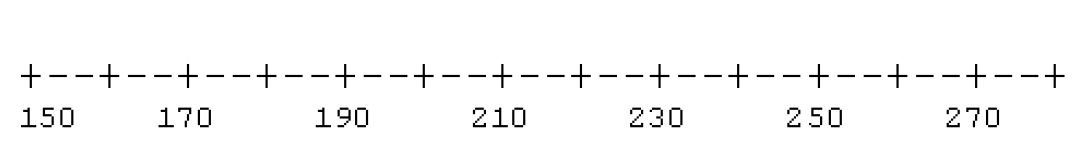
\includegraphics[width=0.8\linewidth]{figures/comparison/boxplot1}

\begin{enumerate}
\def\labelenumi{\arabic{enumi}.}
\setcounter{enumi}{1}
\tightlist
\item
  Draw a box where the lines of the box correspond to the locations of the fourths and the median. (See diagram.)
\end{enumerate}

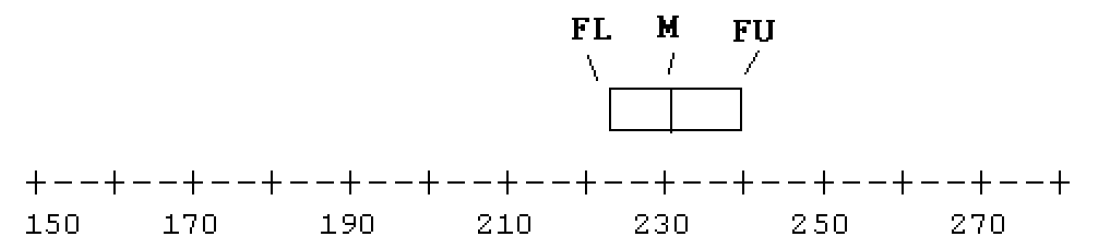
\includegraphics[width=0.8\linewidth]{figures/comparison/boxplot2}

\begin{enumerate}
\def\labelenumi{\arabic{enumi}.}
\setcounter{enumi}{2}
\tightlist
\item
  Indicate the outliers using separate plotting points.
\end{enumerate}

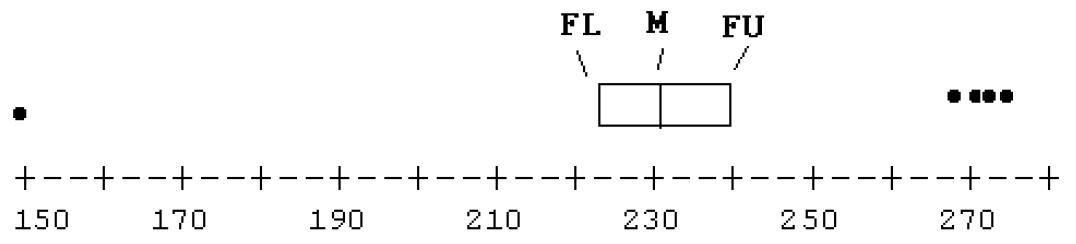
\includegraphics[width=0.8\linewidth]{figures/comparison/boxplot3}

\begin{enumerate}
\def\labelenumi{\arabic{enumi}.}
\setcounter{enumi}{3}
\tightlist
\item
  To complete the box, draw lines out from the box to the most extreme values that are not outliers. (These points are called adjacent values.)
\end{enumerate}

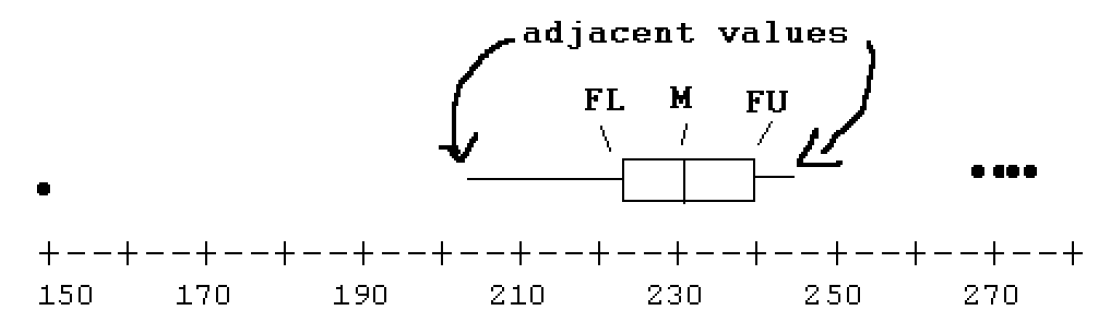
\includegraphics[width=0.8\linewidth]{figures/comparison/boxplot4}

Of course, we don't need our labels and so our boxplot would look like

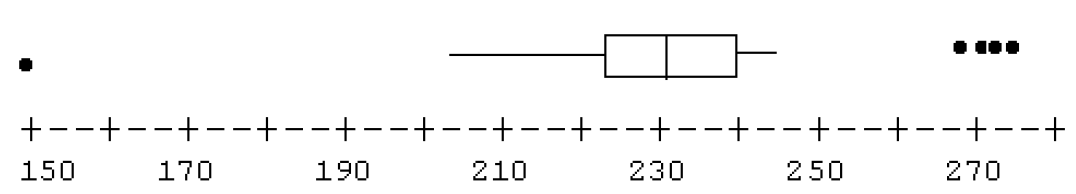
\includegraphics[width=0.8\linewidth]{figures/comparison/boxplot5}

Here is a software generated boxplot display using the \texttt{ggplot2} package in R.

\begin{Shaded}
\begin{Highlighting}[]
\FunctionTok{library}\NormalTok{(LearnEDAfunctions)}
\FunctionTok{library}\NormalTok{(tidyverse)}
\FunctionTok{ggplot}\NormalTok{(}\FunctionTok{filter}\NormalTok{(boston.marathon, age }\SpecialCharTok{==} \DecValTok{20}\NormalTok{),}
       \FunctionTok{aes}\NormalTok{(}\AttributeTok{x =} \DecValTok{1}\NormalTok{, }\AttributeTok{y =}\NormalTok{ time)) }\SpecialCharTok{+} \FunctionTok{xlim}\NormalTok{(}\DecValTok{0}\NormalTok{, }\DecValTok{2}\NormalTok{) }\SpecialCharTok{+}
  \FunctionTok{geom\_boxplot}\NormalTok{() }\SpecialCharTok{+} \FunctionTok{coord\_flip}\NormalTok{() }\SpecialCharTok{+} 
  \FunctionTok{theme}\NormalTok{(}\AttributeTok{axis.title.y=}\FunctionTok{element\_blank}\NormalTok{(),}
        \AttributeTok{axis.text.y=}\FunctionTok{element\_blank}\NormalTok{(),}
        \AttributeTok{axis.ticks.y=}\FunctionTok{element\_blank}\NormalTok{())}
\end{Highlighting}
\end{Shaded}

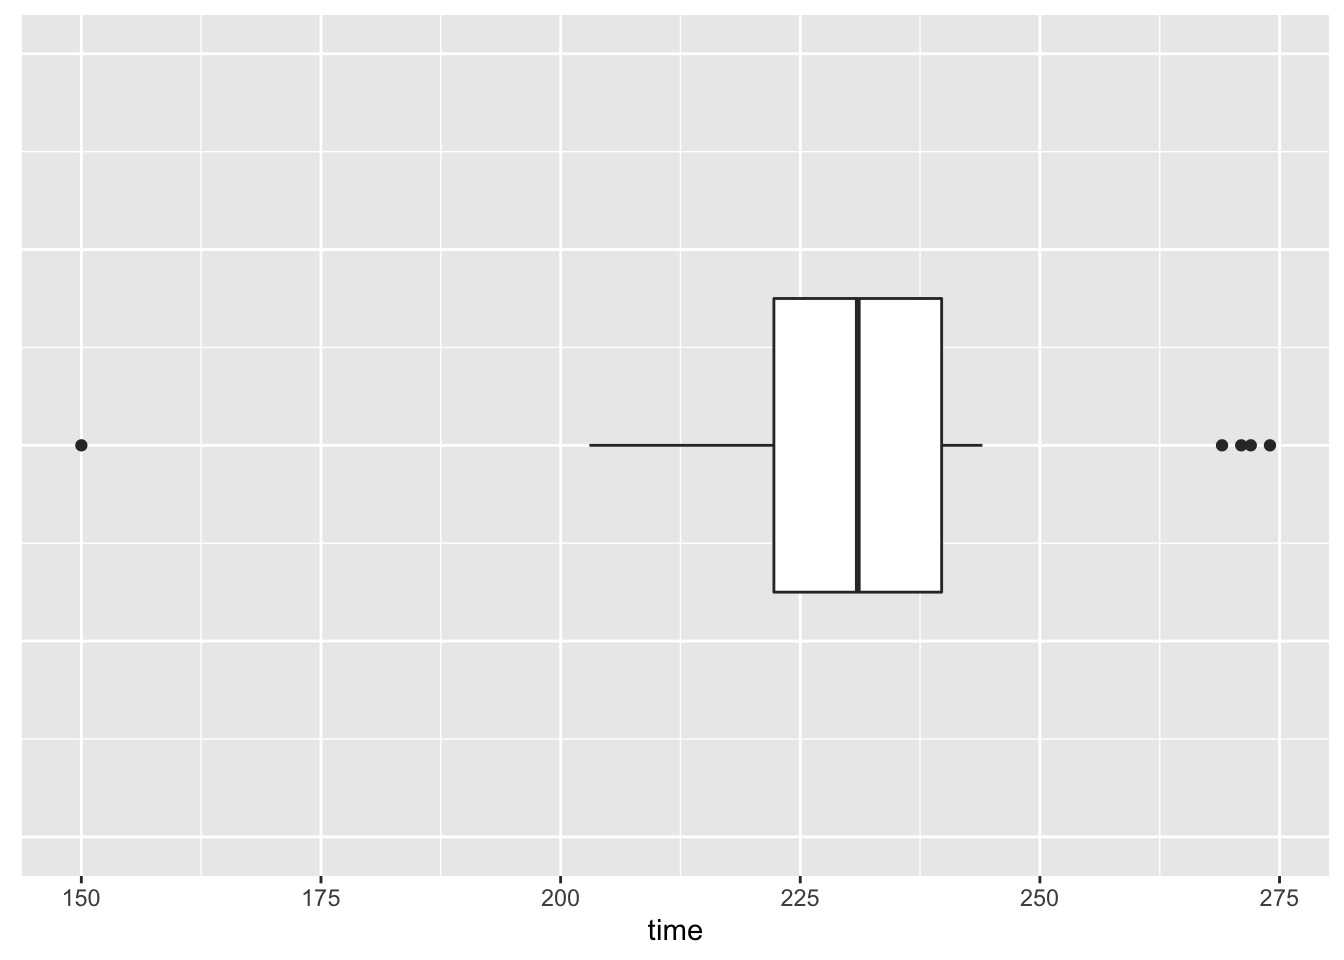
\includegraphics{Course-in-Exploratory-Data-Analysis_files/figure-latex/unnamed-chunk-25-1.pdf}

\hypertarget{interpreting-a-boxplot}{%
\section{Interpreting a Boxplot}\label{interpreting-a-boxplot}}

Before we use boxplots to compare batches, let us spend some time interpreting a boxplot for a single batch. The figure below shows the histogram and corresponding boxplot for two datasets. The first dataset (left side) is symmetric with long tails on both sides.

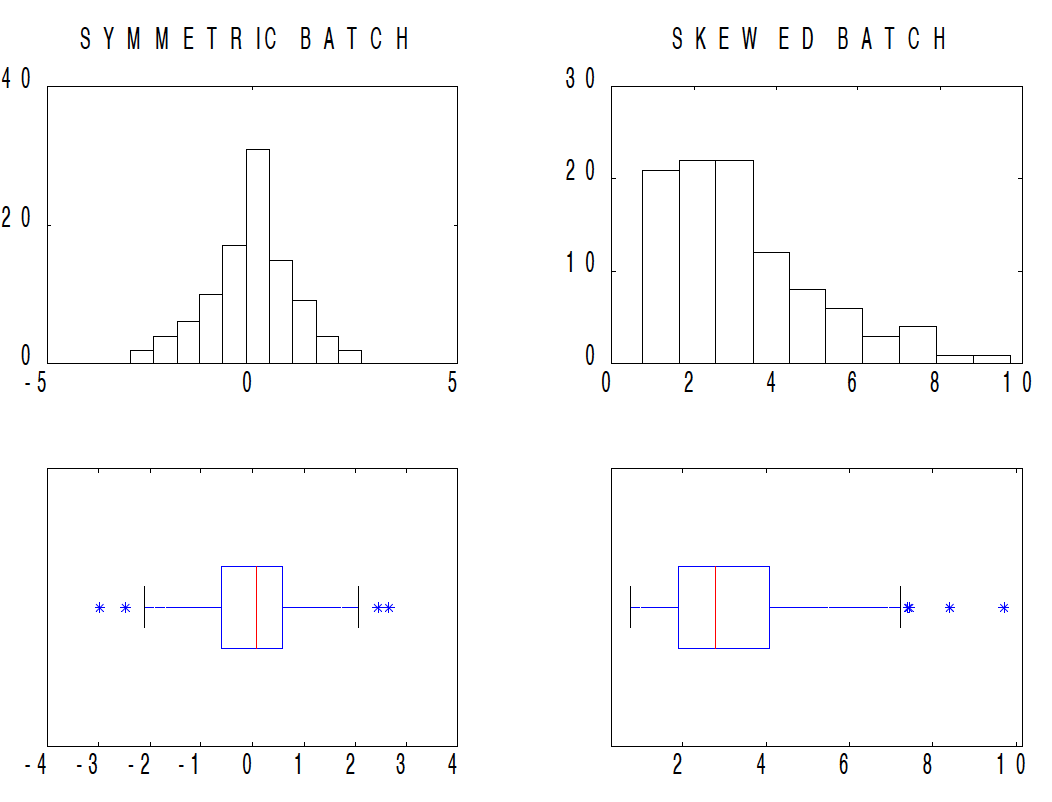
\includegraphics[width=0.8\linewidth]{figures/comparison/boxplot6}

If we look at the corresponding boxplot of this symmetric dataset, we see

\begin{itemize}
\tightlist
\item
  the location of the median (red line) is roughly half-way across the box (the location of the fourths)
\item
  the lengths of the right and left whiskers (the lines extending from the box) are about the same -- this means that the width of the lower quarter of the data is equal to the width of the upper quarter
\end{itemize}

Let's contrast this boxplot of the symmetric batch with the boxplot of the batch on the right. From the histogram, we see that this data is skewed right -- most of the data is in the 0-4 range and the values tail off towards large values. If we look at the corresponding boxplot, we see

\begin{itemize}
\tightlist
\item
  the length of the box from the median to the upper fourth is longer than the length from the lower fourth to the median -- this indicates skewness in the middle half of the data
\item
  the length of the right whisker is significantly longer than the length of the left whisker -- this shows right skewness in the tail portion of the data
\end{itemize}

After some practice looking at boxplots, you'll see that a boxplot is pretty informative about the shape of a batch.

\hypertarget{boxplots-to-compare-batches}{%
\section{Boxplots to Compare Batches}\label{boxplots-to-compare-batches}}

Now we are ready to use boxplots to compare the batches of running times for the different age groups. For each batch, we compute (1) the five-number summary, (2) the fences, and (3) indicate any outliers. Below, we have summarized our calculations for the five age groups, and then we use the calculations to construct boxplots for the batches. We display all of the boxplots on a single plot using one scale.

\begin{verbatim}
Age = 20

      Depth       Lower        Upper                
 N=   22                        
 M    11.5           231.000                
 F     6.0      222.000      240.000        
STEP = 27                       
FENCES = 195, 258                   
OUTLIERS:  150, 269, 271, 272, 274      

Age = 30

        Depth   Lower        Upper 
 N=   25
 M    13.0           235.000         
 F     7.0    213.000      259.000 
STEP = 69
FENCES: 144, 328
OUTLIERS:  330, 346

Age = 40    

      Depth       Lower        Upper  
 N=   25                        
 M    13.0           239.000                    
 F     7.0      224.000      262.000            
STEP = 57                       
FENCES = 167, 319                   
OUTLIERS:  163, 166                 

Age = 50  

      Depth       Lower        Upper
 N=   25
 M    13.0           262.000         
 H     7.0    251.000      281.000 
STEP = 45
FENCES:  206, 326
OUTLIERS:  327, 349

Age = 60

      Depth       Lower        Upper       
 N=   11
 M     6.0           274.000               
 H     3.5      264.000      279.000       
STEP = 22.5
FENCES:  241.5, 301.5
OUTLIERS:  219, 233, 315, 338
\end{verbatim}

\begin{Shaded}
\begin{Highlighting}[]
\FunctionTok{ggplot}\NormalTok{(boston.marathon, }\FunctionTok{aes}\NormalTok{(}\AttributeTok{x =} \FunctionTok{factor}\NormalTok{(age), }\AttributeTok{y =}\NormalTok{ time)) }\SpecialCharTok{+}
  \FunctionTok{geom\_boxplot}\NormalTok{() }\SpecialCharTok{+} \FunctionTok{coord\_flip}\NormalTok{() }\SpecialCharTok{+}
  \FunctionTok{xlab}\NormalTok{(}\StringTok{"Age"}\NormalTok{) }\SpecialCharTok{+} \FunctionTok{ylab}\NormalTok{(}\StringTok{"Time"}\NormalTok{)}
\end{Highlighting}
\end{Shaded}

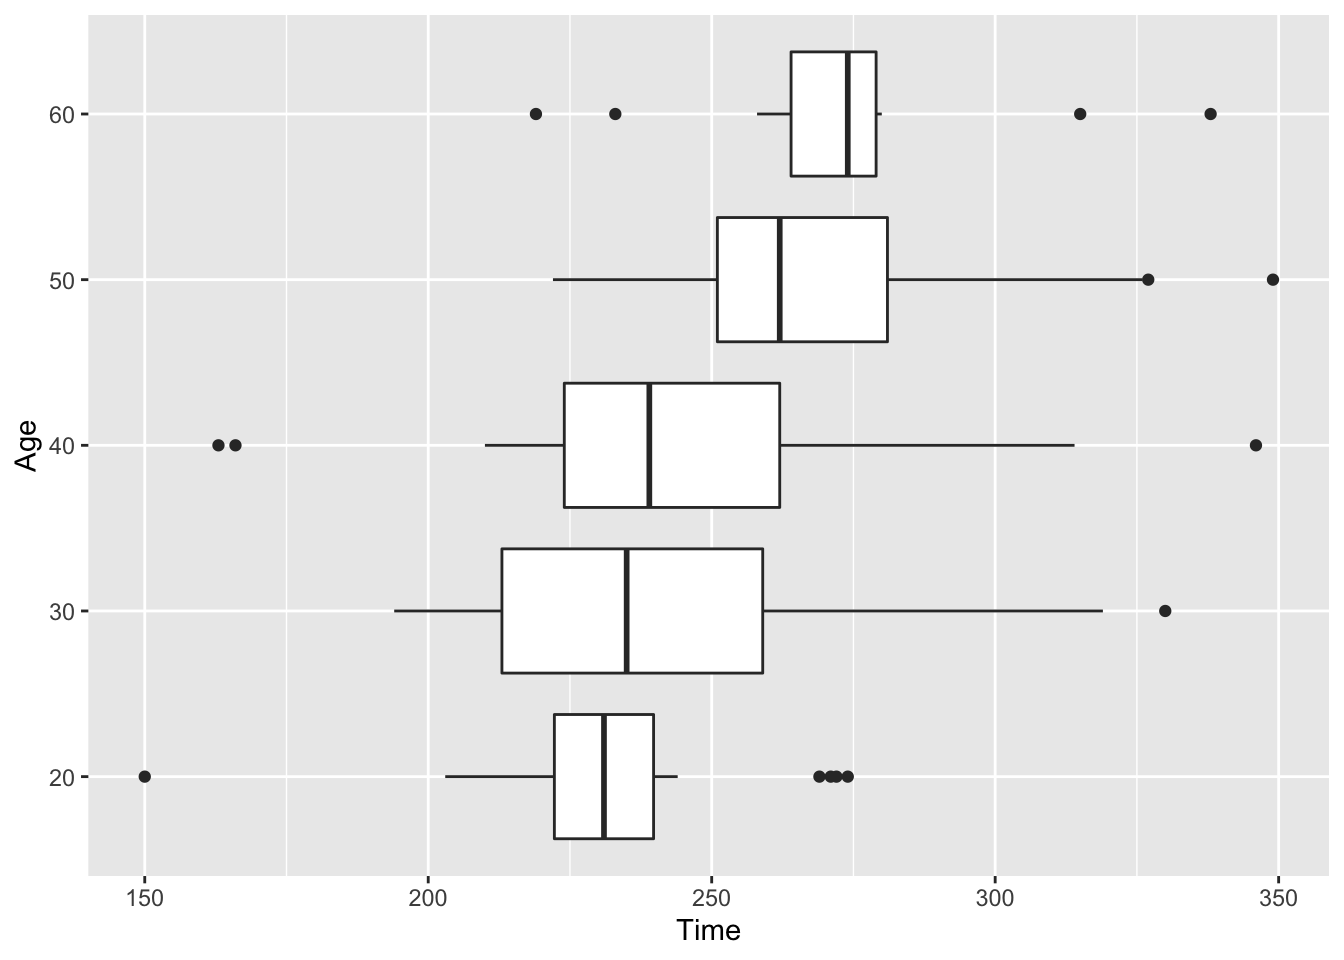
\includegraphics{Course-in-Exploratory-Data-Analysis_files/figure-latex/unnamed-chunk-27-1.pdf}

What do we see in this display of boxplots?

\begin{itemize}
\item
  It is easier to interpret this display when the boxplots are sorted by the medians of the groups. Here this sorting occurs naturally, since the 20 year-olds generally have smaller times than the 30 year-olds, and the 30 year-olds have smaller times for the 40 year-olds, and so on.
\item
  We notice a number of outlying points. In each age group, there are one or two unusually large times. Since we give special recognition to short times, we notice the 20-year woman who ran the race in 150 minutes.
\item
  If we focus on the three middle age groups, we notice that each group has about the same spread. (The spreads of the times for the 20 year-olds and the 60 year-olds are a bit smaller.) The lengths of the boxes for the three groups are about the same, indicating they have similar fourth spreads.
\end{itemize}

\hypertarget{comparisons-using-medians}{%
\section{Comparisons using Medians}\label{comparisons-using-medians}}

When batches have similar spreads, it is easy to make comparisons. Let's illustrate this for the three middle age groups that have similar spreads. The medians and fourth spreads for these batches are

\begin{verbatim}
            Median  Fourth-Spread

age30       235 min 46 min

age40       239 min 38 min

age50       262 min 30 min
\end{verbatim}

Since the times for the 30-year-old and 40-year-old groups have approximately the same spread, the batch of 40-year-old times can be obtained by adding 4 minutes (the difference in medians) to the batch of 30-year-old times. In other words,

\[
age40 = age30 + 4
\]
which means that the 40-year-olds run, on average, 4 minutes longer than the 30-year-older runners.

Similarly, comparing the two older groups, we can say that
\[
age50 = age40 + 23
\]
which means that the batch of 50-year-old times can be found by adding 23 minutes to the 40-year-old times.

Do older women runners run slower than younger women in the Boston Marathon? Looking back at our boxplot display and comparing medians of the five groups, we see that women of ages 20, 30, and 40 have (approximately) the same median completion time. The median time for the 50 year-old runners seems significantly higher that the times for the 20-40 year-olds, and the runners of age 60 have a significantly higher median than the 50-year-olds. So it appears that the best times for women marathoners are in a broad range between 20 and 40 years, and the times don't appear to deteriorate until after age 40.

This is a nice illustration, since the batches of data had similar spreads and this facilitated comparisons by comparing medians. We will see in our next example that batches can have varying spreads and this motivates a reexpression or change in the scale of the data so that the reexpressed batches have similar spreads

\hypertarget{spread-level-plot}{%
\chapter{Spread Level Plot}\label{spread-level-plot}}

\hypertarget{lets-meet-the-data}{%
\section{Let's Meet the Data}\label{lets-meet-the-data}}

The following table displays the population densities of each state in the U.S. for the years 1960, 1970, 1980, 1990, 2000, 2008. Here population density is defined to be the number of people who live in the state per square mile, counting only land area. We know that the U.S. population has been increasing substantially in this last century and since the land area has remained roughly constant, this means that the population densities have been increasing. Our goal here is to effectively compare the six batches of densities to investigate the rate of change in this time period.

\begin{Shaded}
\begin{Highlighting}[]
\FunctionTok{library}\NormalTok{(LearnEDAfunctions)}
\FunctionTok{library}\NormalTok{(tidyverse)}
\NormalTok{pop.densities }\SpecialCharTok{\%\textgreater{}\%} \FunctionTok{select}\NormalTok{(}\SpecialCharTok{{-}}\NormalTok{State) }\SpecialCharTok{\%\textgreater{}\%} \FunctionTok{head}\NormalTok{()}
\end{Highlighting}
\end{Shaded}

\begin{verbatim}
##   Abbrev  y1960  y1970  y1980  y1990 y2000  y2008
## 1     AL  64.37  67.88  76.74  79.62  87.6  91.87
## 2     AK   0.40   0.53   0.70   0.96   1.1   1.20
## 3     AZ  11.46  15.62  23.92  32.26  45.2  57.20
## 4     AR  34.30  36.94  43.91  45.15  51.3  54.84
## 5     CA 100.77 128.05 151.76 191.15 217.2 235.68
## 6     CO  16.91  21.30  27.86  31.76  41.5  47.62
\end{verbatim}

\hypertarget{comparing-batches-in-the-raw-scale}{%
\section{Comparing Batches in the Raw Scale}\label{comparing-batches-in-the-raw-scale}}

We begin by comparing the six batches of population densities (1960, 1970, 1980, 1990, 2000, 2008) using parallel boxplots. Recall our basic construction process:

\begin{itemize}
\tightlist
\item
  we construct stem and leafs for each batch
\item
  we find 5-number summaries of each
\item
  we set fences for each batch and identify outliers
\item
  we construct parallel boxplots, ordering by the median value.
\end{itemize}

I had R construct the boxplots -- here's the display:

\begin{Shaded}
\begin{Highlighting}[]
\NormalTok{pop.densities }\SpecialCharTok{\%\textgreater{}\%} \FunctionTok{select}\NormalTok{(}\SpecialCharTok{{-}}\NormalTok{State, }\SpecialCharTok{{-}}\NormalTok{Abbrev) }\SpecialCharTok{\%\textgreater{}\%} 
   \FunctionTok{gather}\NormalTok{(Year, Time) }\OtherTok{{-}\textgreater{}}\NormalTok{ stacked.data}
\FunctionTok{ggplot}\NormalTok{(stacked.data, }\FunctionTok{aes}\NormalTok{(Year, Time)) }\SpecialCharTok{+}
  \FunctionTok{geom\_boxplot}\NormalTok{() }\SpecialCharTok{+} \FunctionTok{coord\_flip}\NormalTok{()}
\end{Highlighting}
\end{Shaded}

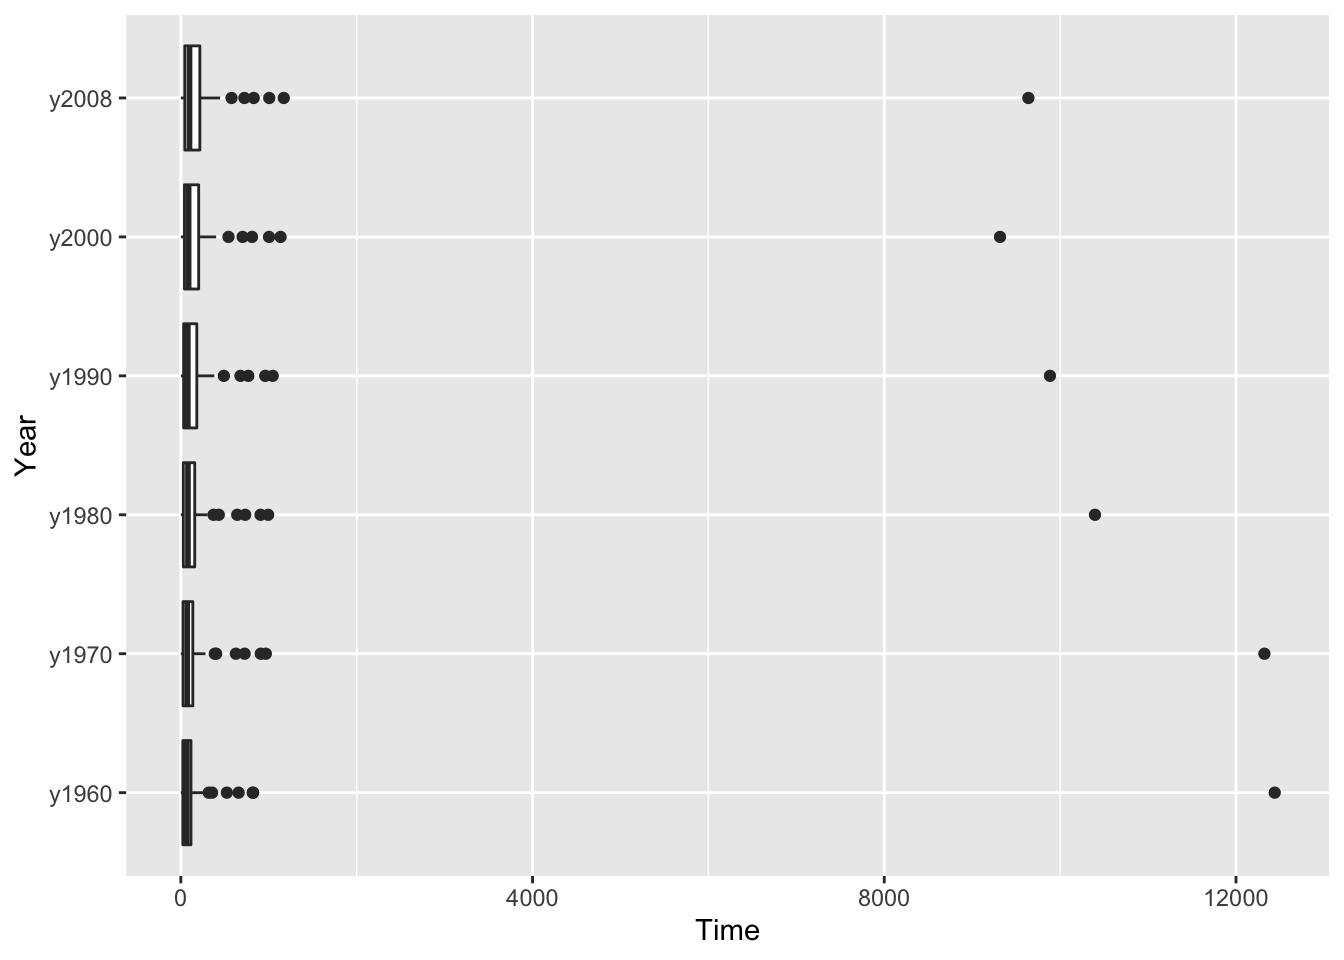
\includegraphics{Course-in-Exploratory-Data-Analysis_files/figure-latex/unnamed-chunk-29-1.pdf}

\hypertarget{whats-wrong}{%
\section{What's Wrong?}\label{whats-wrong}}

It's hard to compare the six batches of densities. Why?

\begin{itemize}
\item
  Each batch is strongly right-skewed. The length of the right tail is longer than the length of the left tail (look at the lengths of the whiskers) and there are a number of outliers at the high end.
\item
  The batches have different spreads. If we look at the length of the boxes (the fourth spread), we see that the 2008 data is more spread out than the 1980 data which is more spread out than the 1960 data.
\item
  Looking further, we see a tendency for the batches of larger densities to have larger spreads. This is obvious if you compare the 2008 densities (large median and large spread) with the 1960 densities (smaller median and smaller spread).
\item
  In other words, we see a dependence between spread and level in this boxplot display.
\end{itemize}

It is difficult to compare these batches since they have unequal spreads. This is a common problem. If we have several batches that contain positive values (like counts or amounts), the batches with larger values will tend also to have larger spreads.

\hypertarget{the-spread-vs-level-plot}{%
\section{The Spread vs Level Plot}\label{the-spread-vs-level-plot}}

We can see the relationship between the averages and spreads by use of a spread vs.~level plot. For each batch, we compute the median \(M\) and the fourth spread \(d_F\). Then we construct a scatterplot of the (\(\log M, \log d_F\)) values. (In this class, we will generally take logs to the base 10 power. Actually, it doesn't make any difference in most settings what type of log we take, but it is easier to interpret a base 10 log.)

The work for the spread vs level plot for our example is shown in the table below. For each batch, we list the median and the fourth spreads and the corresponding logs. Then we plot log M against log df.

\begin{Shaded}
\begin{Highlighting}[]
\FunctionTok{spread\_level\_plot}\NormalTok{(stacked.data, Time, Year)}
\end{Highlighting}
\end{Shaded}

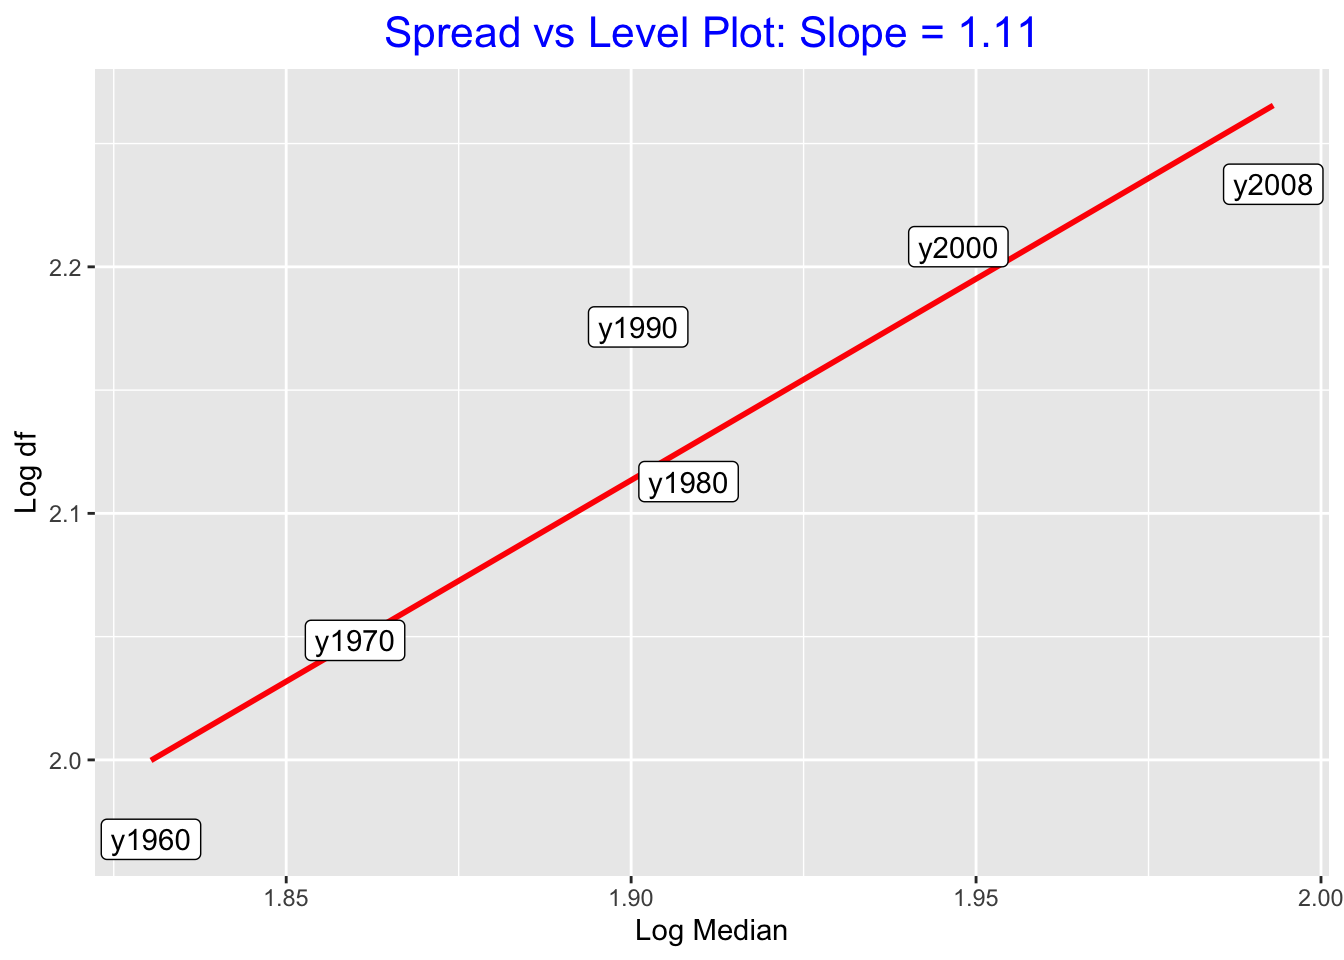
\includegraphics{Course-in-Exploratory-Data-Analysis_files/figure-latex/unnamed-chunk-30-1.pdf}

\begin{verbatim}
## # A tibble: 6 x 5
##   Year      M    df log.M log.df
##   <chr> <dbl> <dbl> <dbl>  <dbl>
## 1 y1960  67.7  92.8  1.83   1.97
## 2 y1970  72.4 112.   1.86   2.05
## 3 y1980  81.0 130.   1.91   2.11
## 4 y1990  79.6 150.   1.90   2.18
## 5 y2000  88.6 161.   1.95   2.21
## 6 y2008  98.4 171.   1.99   2.23
\end{verbatim}

Clearly there is a positive association in the graph, indicating that batches with small medians tend also to have small dfs (spreads).

\hypertarget{reexpression}{%
\section{Reexpression}\label{reexpression}}

We can correct the dependence between spread and level by reexpressing the data to a different scale. We focus on a special case of reexpressions, called power transformations, that have the form
\[
 data^p,
 \]
where \(p\) is the power of the transformation. If \(p = 1\), we just have the raw or original scale. The idea here is to choose a value of \(p\) not equal to 1 that might help in removing the dependence between spread and level.

Here is a simple algorithm to find the power \(p\).

\begin{enumerate}
\def\labelenumi{\arabic{enumi}.}
\tightlist
\item
  Find the medians and fourth-spreads for all batches and compute
  \(\log M\) and \(\log d_F\).
\item
  Construct a scatterplot of \(\log M\) against \(\log d_F\).
  (we're already done the first two steps)
\item
  Fit a line by eye that goes through the points. (There can be some danger in fitting a least-squares line -- we'll explain this problem later.)
\item
  If \(b\) is the slope of the best line, then the power of the reexpression will be
  \[
  p = 1 - b.
  \]
\end{enumerate}

In the spread versus plot of \((\log M, \log d_F)\), a best line is drawn on top.
The slope of the line (as shown in the plot) is b = 1.7. So the power of the reexpression is
\[
p = 1 - b = 1 - 1.7 = -0.7 ,
\]
which is approximately \(-0.5\).
So this method suggests that we should reexpress the density data by taking a \(-0.5\) power.

\hypertarget{reanalysis-of-the-data-in-new-scale}{%
\section{Reanalysis of the data in new scale}\label{reanalysis-of-the-data-in-new-scale}}

Let's check if this method works. We redo our comparison of the 1960, 1970, 1980, 1990, 2000, 2008 batches using the data

\begin{Shaded}
\begin{Highlighting}[]
\NormalTok{stacked.data }\SpecialCharTok{\%\textgreater{}\%} 
  \FunctionTok{mutate}\NormalTok{(}\AttributeTok{Reexpressed =}\NormalTok{ Time }\SpecialCharTok{\^{}}\NormalTok{ (}\SpecialCharTok{{-}}\FloatTok{0.5}\NormalTok{)) }\OtherTok{{-}\textgreater{}}
\NormalTok{  stacked.data}
\FunctionTok{ggplot}\NormalTok{(stacked.data, }\FunctionTok{aes}\NormalTok{(Year, Reexpressed)) }\SpecialCharTok{+}
  \FunctionTok{geom\_boxplot}\NormalTok{() }\SpecialCharTok{+} \FunctionTok{coord\_flip}\NormalTok{()}
\end{Highlighting}
\end{Shaded}

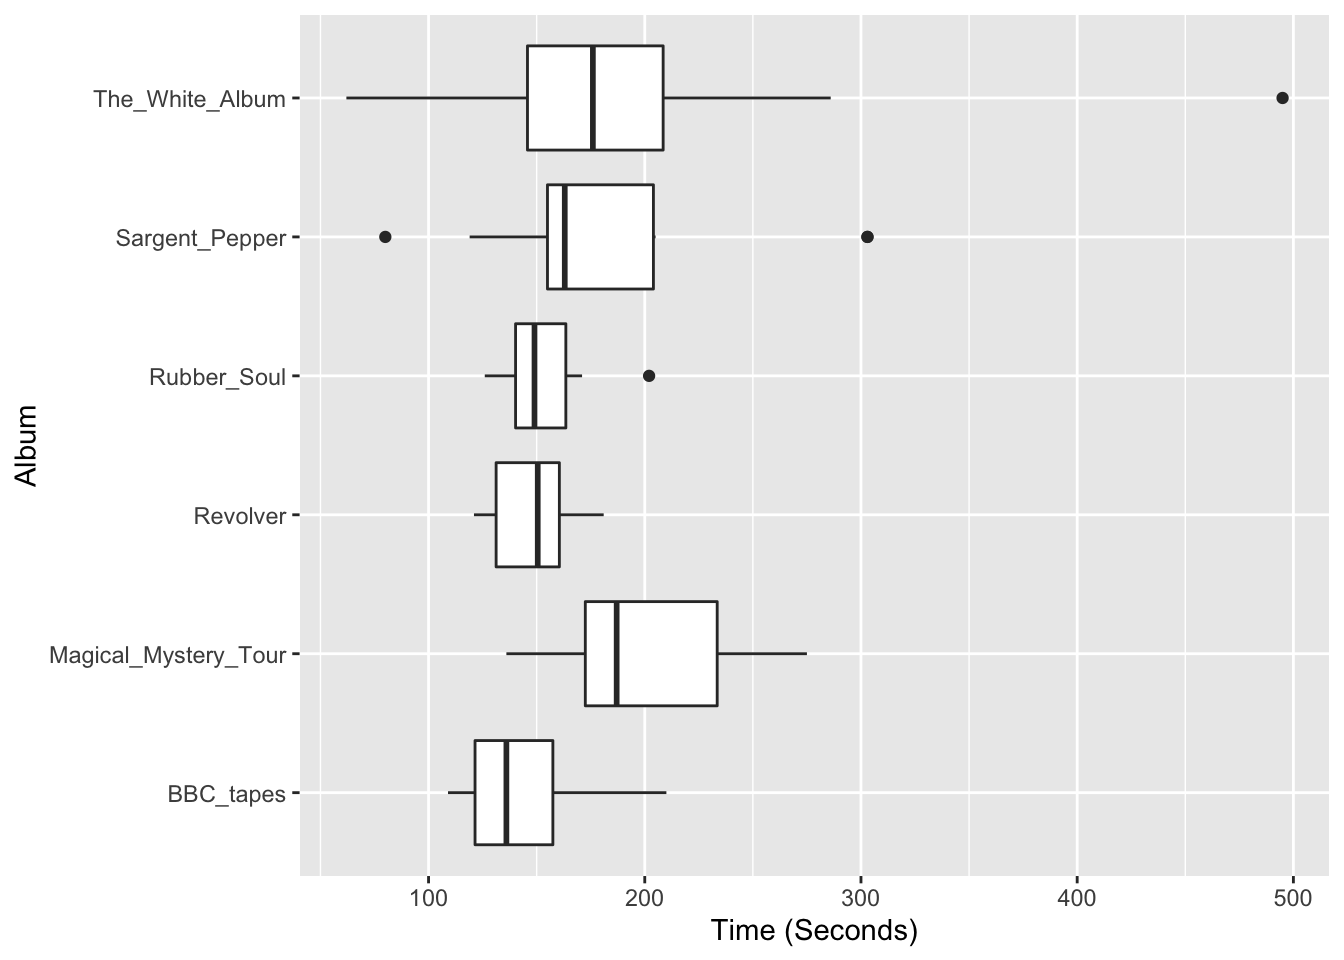
\includegraphics{Course-in-Exploratory-Data-Analysis_files/figure-latex/unnamed-chunk-31-1.pdf}

Actually this display doesn't look much better than our original picture. There is still right skewness in each batch and we can't help but notice the number of high outliers.

But there is one improvement -- the spreads of the middle half of each batch are roughly equal and we have removed the dependence between level and spread.

We can check out this point by performing a spread vs.~level plot for the reexpressed data. In the table, we've listed the median \(M\) and the fourth spread \(d_F\) for the rexpressed data and computed the logs of \(M\) and \(d_F\). We look at a scatterplot of log \(M\) against log \(d_F\) for the reexpressed data.

\begin{Shaded}
\begin{Highlighting}[]
\FunctionTok{spread\_level\_plot}\NormalTok{(stacked.data, Reexpressed, Year)}
\end{Highlighting}
\end{Shaded}

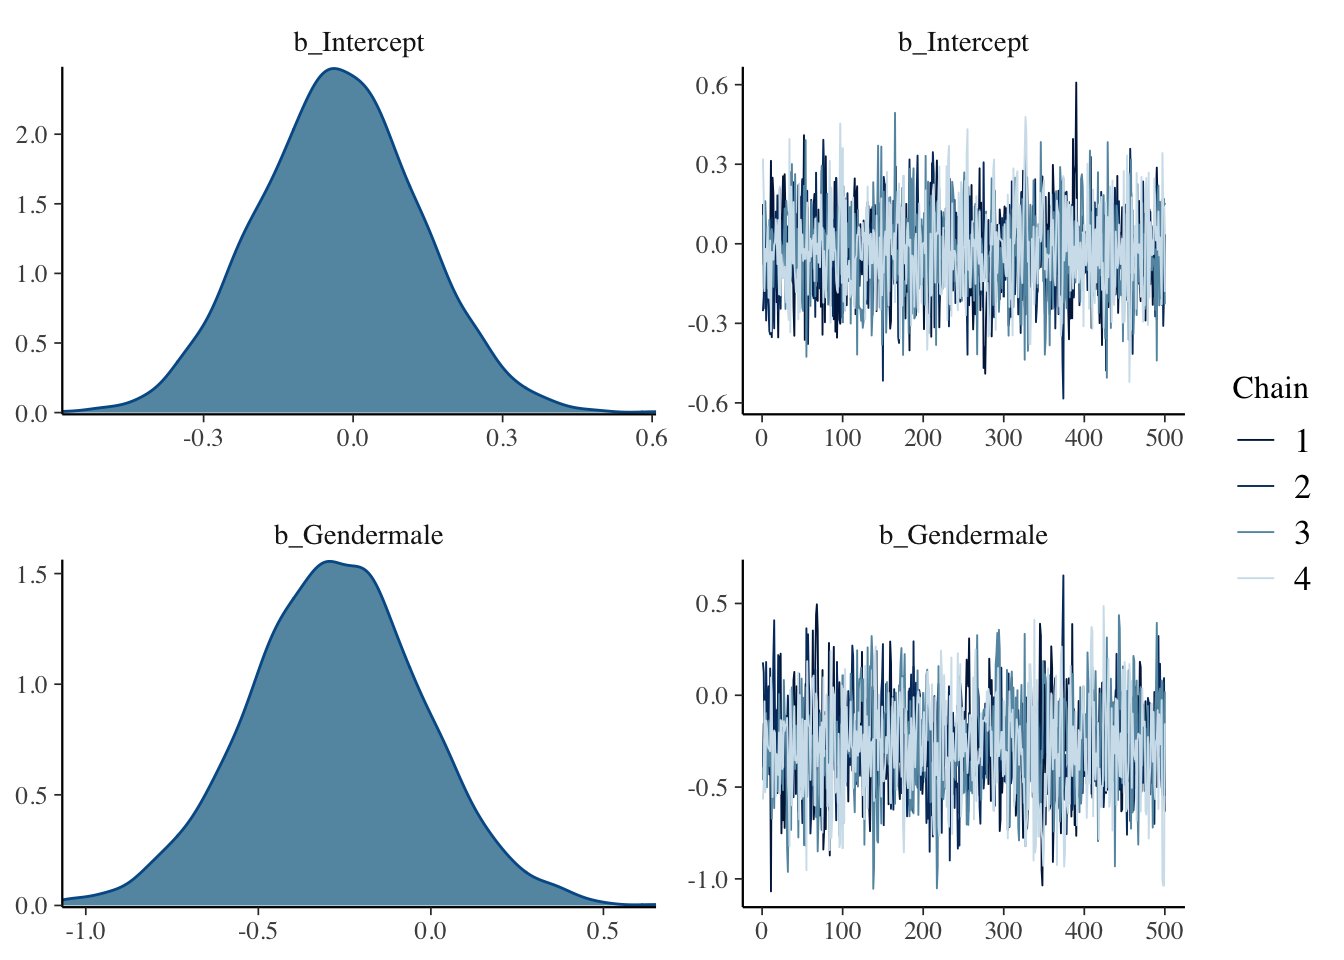
\includegraphics{Course-in-Exploratory-Data-Analysis_files/figure-latex/unnamed-chunk-32-1.pdf}

\begin{verbatim}
## # A tibble: 6 x 5
##   Year      M     df  log.M log.df
##   <chr> <dbl>  <dbl>  <dbl>  <dbl>
## 1 y1960 0.122 0.120  -0.915 -0.922
## 2 y1970 0.117 0.117  -0.930 -0.933
## 3 y1980 0.111 0.108  -0.954 -0.966
## 4 y1990 0.112 0.103  -0.951 -0.989
## 5 y2000 0.106 0.0851 -0.974 -1.07 
## 6 y2008 0.101 0.0809 -0.997 -1.09
\end{verbatim}

Actually, we still see a positive relationship between level and spread, which indicates that a further reexpression may be needed to remove or, at least, decrease the relationship between level and spread. (One can show that reexpressing the data by a 0.1 power seems to do a better job in reducing the dependence between spread and level.)

\hypertarget{wrap-up}{%
\section{Wrap Up}\label{wrap-up}}

What have we learned?

\begin{itemize}
\tightlist
\item
  Batches are harder to compare when they have unequal spreads.
\item
  The goal is to reexpress the data by a power transformation so that the reexpressed data has equal spreads across batches.
\item
  We have introduced a simple plot (spread vs.~level) which is designed to find the correct choice of the power p to accomplish our goal.
\item
  However, this method may not work, and so we should reanalyze our data using the reexpression to see if the dependence between spread and level is reduced.
\end{itemize}

\hypertarget{comparing-batches-iii}{%
\chapter{Comparing Batches III}\label{comparing-batches-iii}}

\hypertarget{a-case-study-where-the-spread-vs-level-plot-works}{%
\section{A Case Study where the Spread vs Level Plot Works}\label{a-case-study-where-the-spread-vs-level-plot-works}}

\textbf{Baseball data: Team homerun numbers for years 1900, \ldots, 2000.}

Background: In baseball, the most dramatic play is the home run, where the batter hits the pitch over the outfield fence. In a current typical baseball game, you may see 1-3 home runs hit. Home runs were not always so common. Here we compare the quantity of home runs hit over the years. Specifically, we look at the total numbers of home runs hit by all teams in the Major League for the years 1900, 1910, \ldots, 2000.

To compare these 11 batches, we use parallel boxplots. In the \texttt{LearnEDA} package, the data is available in the data frame \texttt{homeruns.2000.}
The boxplot function is used to construct parallel boxplots of the team home runs by year.

\begin{Shaded}
\begin{Highlighting}[]
\FunctionTok{library}\NormalTok{(LearnEDAfunctions)}
\FunctionTok{library}\NormalTok{(tidyverse)}
\FunctionTok{ggplot}\NormalTok{(homeruns}\FloatTok{.2000}\NormalTok{, }\FunctionTok{aes}\NormalTok{(}\FunctionTok{factor}\NormalTok{(YEARS), HOMERUNS)) }\SpecialCharTok{+}
  \FunctionTok{geom\_boxplot}\NormalTok{() }\SpecialCharTok{+} \FunctionTok{coord\_flip}\NormalTok{() }\SpecialCharTok{+}
  \FunctionTok{xlab}\NormalTok{(}\StringTok{"Year"}\NormalTok{)}
\end{Highlighting}
\end{Shaded}

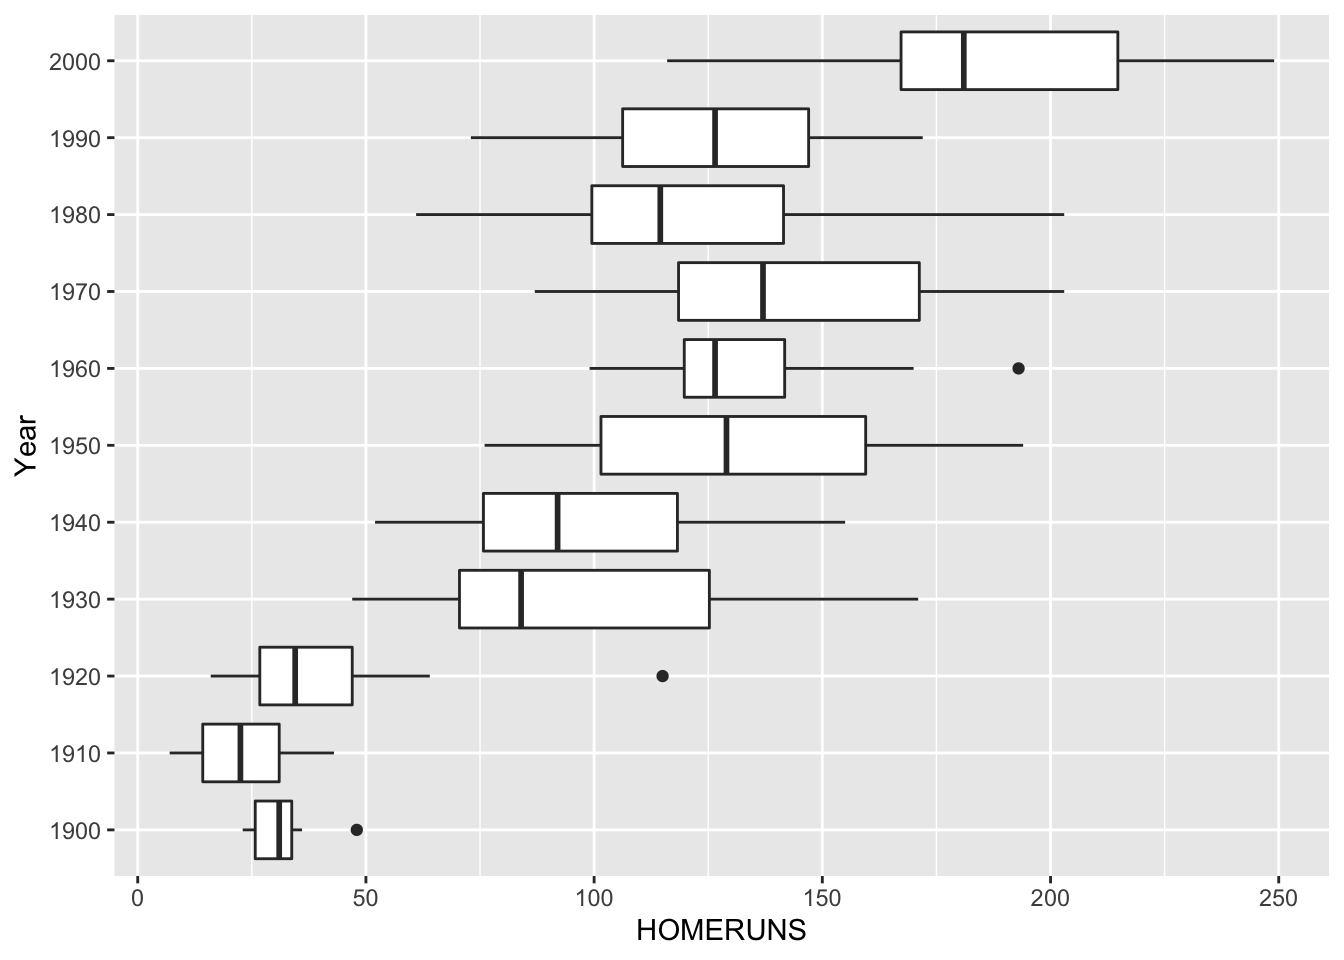
\includegraphics{Course-in-Exploratory-Data-Analysis_files/figure-latex/unnamed-chunk-33-1.pdf}

Looking at this graph, what do we see?

\begin{itemize}
\tightlist
\item
  We see that there were a small number of home runs hit by teams in the early years (1900-1920) compared with the later years (1930-2000).
\item
  Also the spreads of the batches are not the same. The batches with the small home run numbers are also the ones with the smallest spreads.
\item
  So there appears to be a dependence between spread and level here.
\end{itemize}

To construct a spread vs.~level plot, we apply the R function spread.level.plot. This function output a tables of the medians, dfs, log10(medians), log10(dfs) for all years. Also it constructs a spread versus level graph with a ``best line'' line superimposed.

\begin{Shaded}
\begin{Highlighting}[]
\FunctionTok{spread\_level\_plot}\NormalTok{(homeruns}\FloatTok{.2000}\NormalTok{, HOMERUNS, YEARS)}
\end{Highlighting}
\end{Shaded}

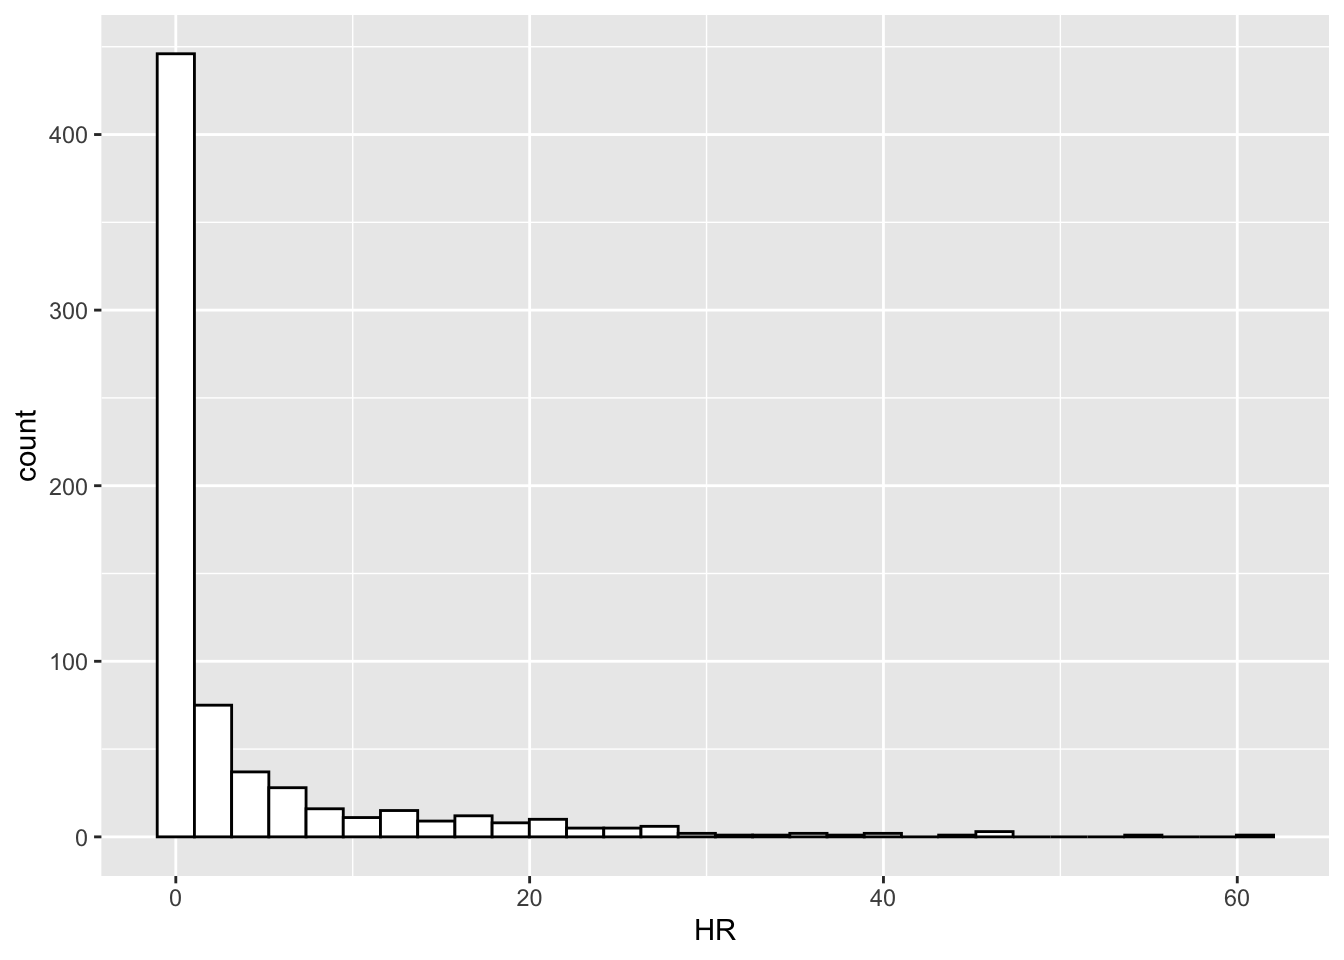
\includegraphics{Course-in-Exploratory-Data-Analysis_files/figure-latex/unnamed-chunk-34-1.pdf}

\begin{verbatim}
## # A tibble: 11 x 5
##    YEARS     M    df log.M log.df
##    <int> <dbl> <dbl> <dbl>  <dbl>
##  1  1900  31     8    1.49  0.903
##  2  1910  22.5  16.8  1.35  1.22 
##  3  1920  34.5  20.2  1.54  1.31 
##  4  1930  84    54.8  1.92  1.74 
##  5  1940  92    42.5  1.96  1.63 
##  6  1950 129    58    2.11  1.76 
##  7  1960 126.   22    2.10  1.34 
##  8  1970 137    52.8  2.14  1.72 
##  9  1980 114.   42    2.06  1.62 
## 10  1990 126.   40.8  2.10  1.61 
## 11  2000 181    47.5  2.26  1.68
\end{verbatim}

We see a positive association in the graph, indicating a dependence between level (measured by \(\log M\)) and spread (measured by \(\log d_F)\).

We fit a line to this graph. We use a resistant procedure called ``resistant line'' to fit this line (we'll talk more about this procedure later in this course). The slope of this line is \(b = .64\). So, by using our rule-of-thumb, we should reexpress our home run data by a power transformation with power \(p = 1 - b = 1 - .64\) which is approximately \(p = .5\). In other words, this method suggests taking a root transformation.

On R, we create a new variable roots that will contain the square roots of the home run numbers.

\begin{Shaded}
\begin{Highlighting}[]
\NormalTok{homeruns}\FloatTok{.2000} \SpecialCharTok{\%\textgreater{}\%} \FunctionTok{mutate}\NormalTok{(}\AttributeTok{roots =} \FunctionTok{sqrt}\NormalTok{(HOMERUNS)) }\OtherTok{{-}\textgreater{}}
\NormalTok{  homeruns}\FloatTok{.2000}
\end{Highlighting}
\end{Shaded}

We construct a parallel boxplot display of the batches of root home run numbers.

\begin{Shaded}
\begin{Highlighting}[]
\FunctionTok{ggplot}\NormalTok{(homeruns}\FloatTok{.2000}\NormalTok{, }\FunctionTok{aes}\NormalTok{(}\FunctionTok{factor}\NormalTok{(YEARS), roots)) }\SpecialCharTok{+}
  \FunctionTok{geom\_boxplot}\NormalTok{() }\SpecialCharTok{+} \FunctionTok{coord\_flip}\NormalTok{() }\SpecialCharTok{+}
  \FunctionTok{xlab}\NormalTok{(}\StringTok{"Year"}\NormalTok{)}
\end{Highlighting}
\end{Shaded}

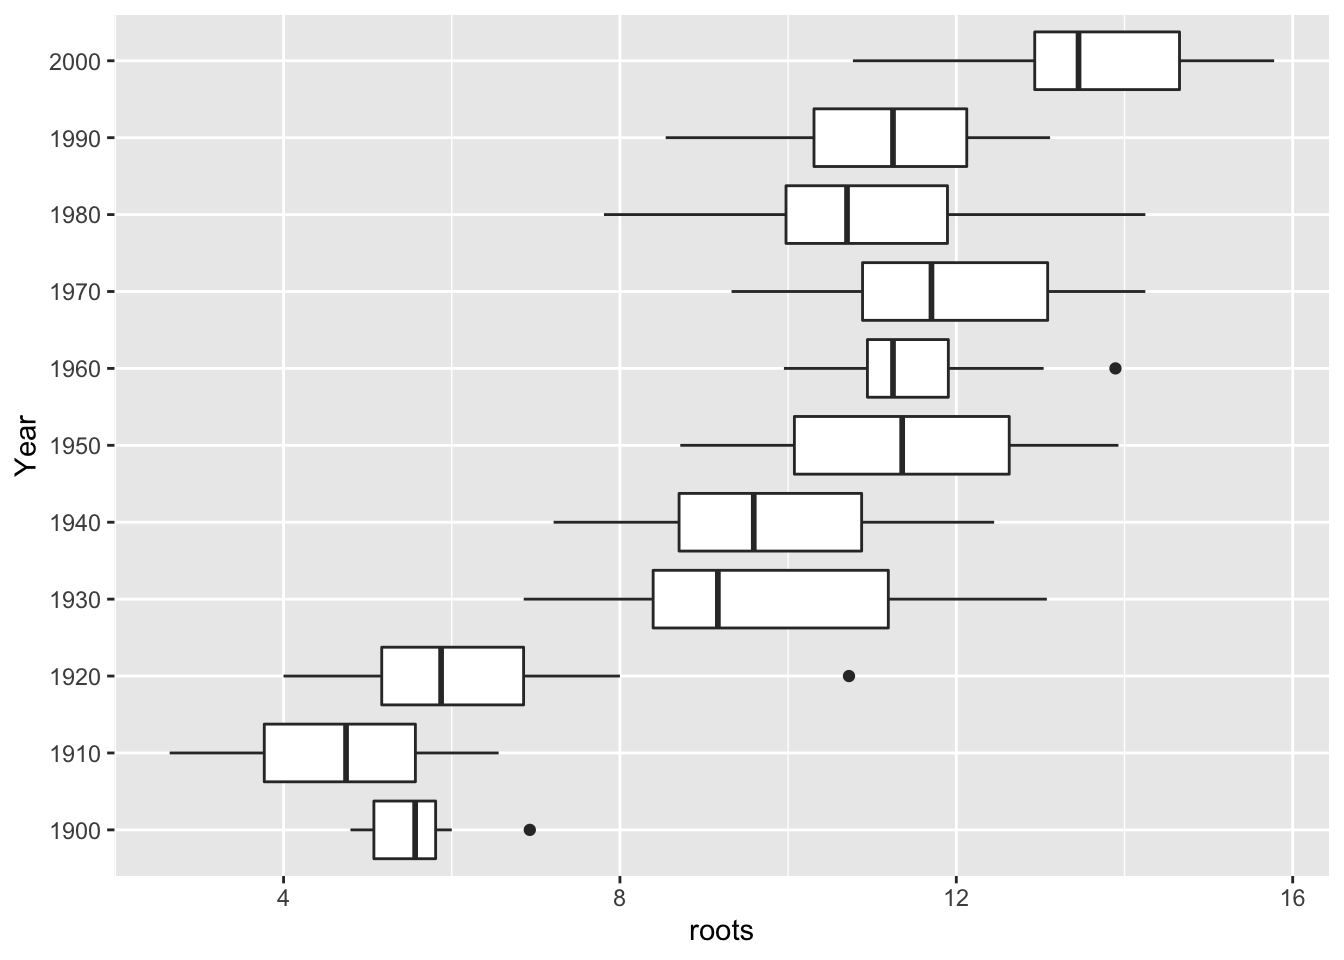
\includegraphics{Course-in-Exploratory-Data-Analysis_files/figure-latex/unnamed-chunk-36-1.pdf}

This plot looks better -- the spreads of the batches are more similar. The batches with the smallest home run counts (1900-1920) have spreads that are similar in size to the spreads of the batches with large counts.

If you perform a spread vs.~level plot of this reexpressed data (that is, the root data), you won't see much of a relationship between \(\log M\) and \(\log d_F\). (Remember, \(M\) and \(d_F\) are computed using the root home run data.)

\hypertarget{a-case-study-where-the-spread-vs-level-plot-doesnt-work}{%
\section{A Case Study where the Spread vs Level Plot Doesn't Work}\label{a-case-study-where-the-spread-vs-level-plot-doesnt-work}}

\textbf{Music Data: Time in seconds of tracks of the Fab Four}

Background: The Beatles were a famous pop group that played in the 60's and 70's. The style of the Beatles' music changed over their career -- this change in style is reflected by the length of their songs.

We look at six Beatles' albums: The BBC Tapes, Rubber Soul, Revolver, Magical Mystery Tour, Sgt.~Pepper, and The White Album. For each album, we measure the time (in seconds) for all of the songs. The data is stored in the \texttt{LearnEDA} data frame \texttt{beatles}.

\begin{Shaded}
\begin{Highlighting}[]
\FunctionTok{ggplot}\NormalTok{(beatles, }\FunctionTok{aes}\NormalTok{(album, time)) }\SpecialCharTok{+}
  \FunctionTok{geom\_boxplot}\NormalTok{() }\SpecialCharTok{+} \FunctionTok{coord\_flip}\NormalTok{() }\SpecialCharTok{+}
  \FunctionTok{xlab}\NormalTok{(}\StringTok{"Album"}\NormalTok{) }\SpecialCharTok{+}
  \FunctionTok{ylab}\NormalTok{(}\StringTok{"Time (Seconds)"}\NormalTok{)}
\end{Highlighting}
\end{Shaded}

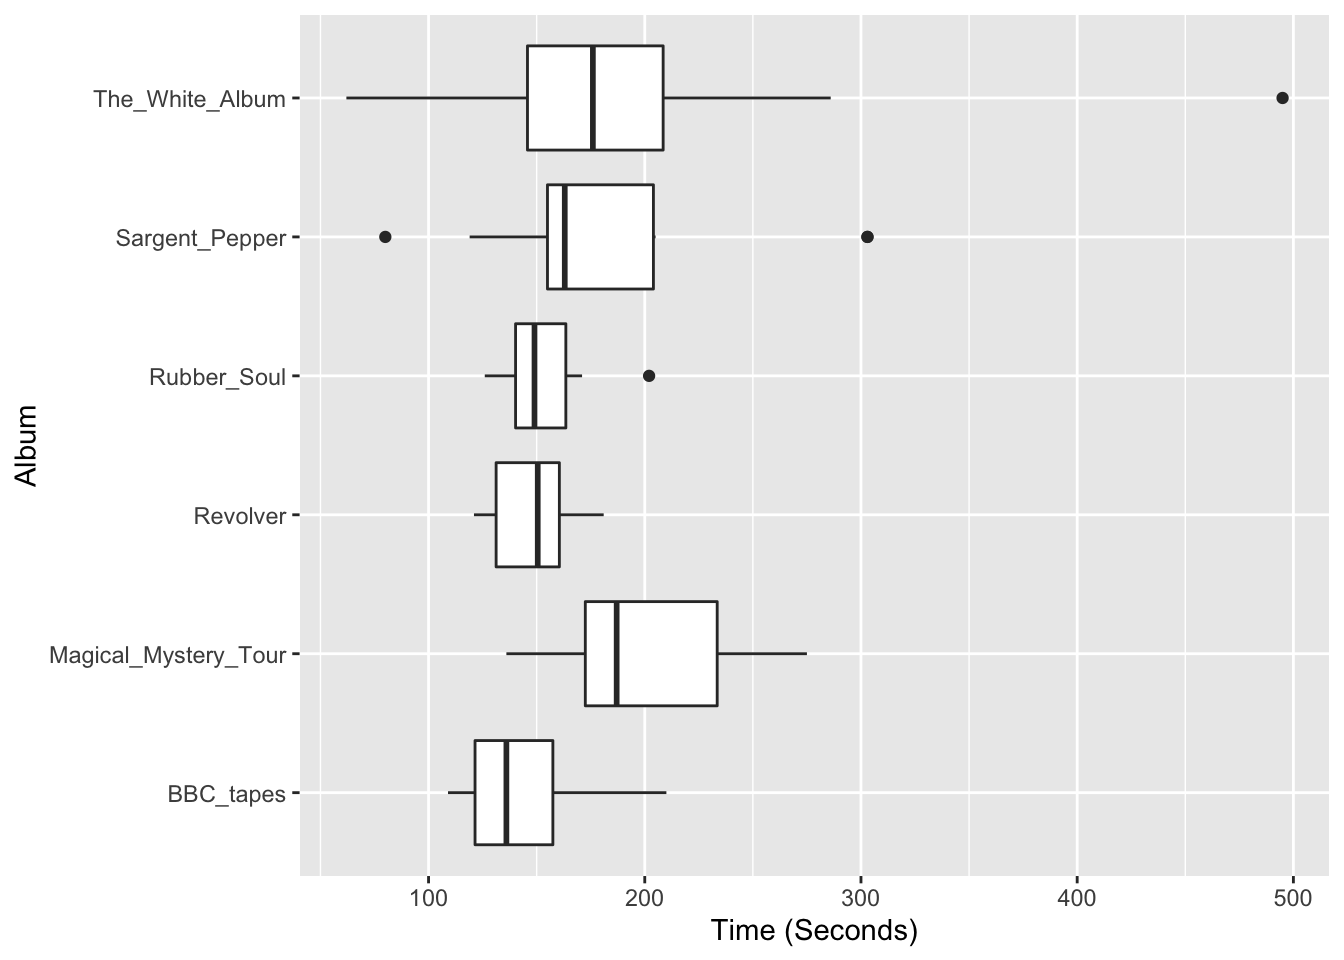
\includegraphics{Course-in-Exploratory-Data-Analysis_files/figure-latex/unnamed-chunk-37-1.pdf}

Here are parallel boxplots of the times of the songs on the six albums. We see differences in the average song lengths -- Magical Mystery Tour and The White Album tend to have longer songs than Rubber Soul and Revolver. But we also see differences in the spreads of the batches and so we try our spread vs.~level plot to suggest a possible reexpression of the data.

The table below shows the medians, fourth-spreads, and logs for the six batches, followed by a spread vs level plot.

\begin{Shaded}
\begin{Highlighting}[]
\FunctionTok{spread\_level\_plot}\NormalTok{(beatles, time, album)}
\end{Highlighting}
\end{Shaded}

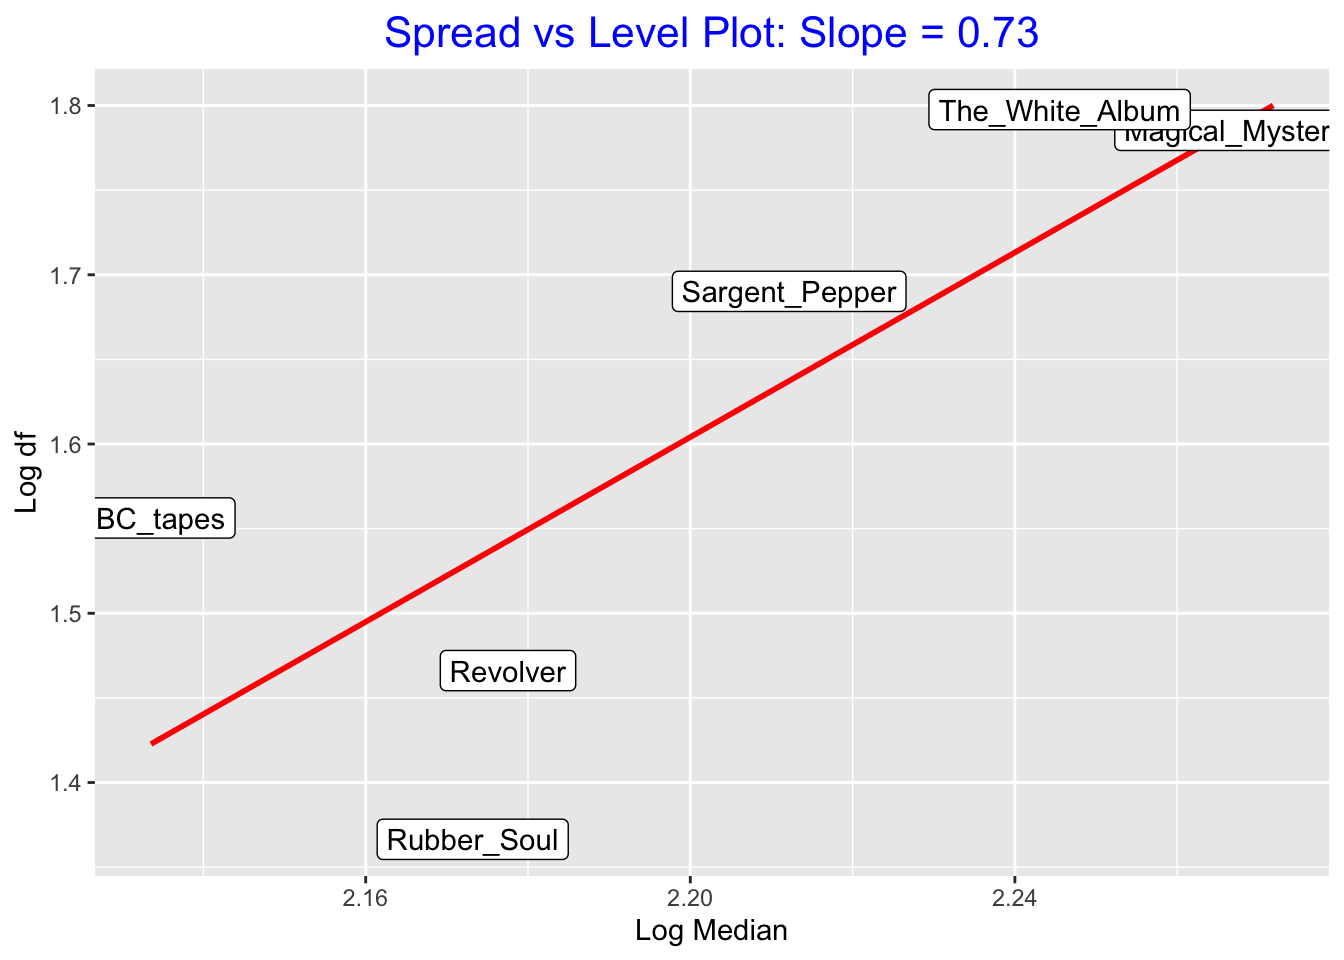
\includegraphics{Course-in-Exploratory-Data-Analysis_files/figure-latex/unnamed-chunk-38-1.pdf}

\begin{verbatim}
## # A tibble: 6 x 5
##   album                    M    df log.M log.df
##   <fct>                <dbl> <dbl> <dbl>  <dbl>
## 1 BBC_tapes             136   36    2.13   1.56
## 2 Magical_Mystery_Tour  187   61    2.27   1.79
## 3 Revolver              150.  29.2  2.18   1.47
## 4 Rubber_Soul           149   23.2  2.17   1.37
## 5 Sargent_Pepper        163   49    2.21   1.69
## 6 The_White_Album       176   62.8  2.25   1.80
\end{verbatim}

We see a positive association in this plot -- a resistant fit to this graph gives a slope of 3.1 which suggests a power of \(p = 1 - 3.1 = -2.1\) which is approximately equal to \(-2\).

We try out this reexpression -- we transform the time data to \((time)^{-2}\). The first graph shows parallel boxplots of \((time)^{-2}\); the second graph does a spread vs.~level plot for this reexpressed data.

\begin{Shaded}
\begin{Highlighting}[]
\NormalTok{beatles }\SpecialCharTok{\%\textgreater{}\%} 
  \FunctionTok{mutate}\NormalTok{(}\AttributeTok{New =} \DecValTok{10} \SpecialCharTok{*}\NormalTok{ (time) }\SpecialCharTok{\^{}}\NormalTok{ (}\SpecialCharTok{{-}}\DecValTok{2}\NormalTok{)) }\OtherTok{{-}\textgreater{}}
\NormalTok{  beatles}
\FunctionTok{ggplot}\NormalTok{(beatles, }\FunctionTok{aes}\NormalTok{(album, New)) }\SpecialCharTok{+}
  \FunctionTok{geom\_boxplot}\NormalTok{() }\SpecialCharTok{+}
  \FunctionTok{coord\_flip}\NormalTok{() }\SpecialCharTok{+} \FunctionTok{xlab}\NormalTok{(}\StringTok{"ALBUM"}\NormalTok{) }\SpecialCharTok{+}
  \FunctionTok{ylab}\NormalTok{(}\StringTok{"Reexpressed Data"}\NormalTok{)}
\end{Highlighting}
\end{Shaded}

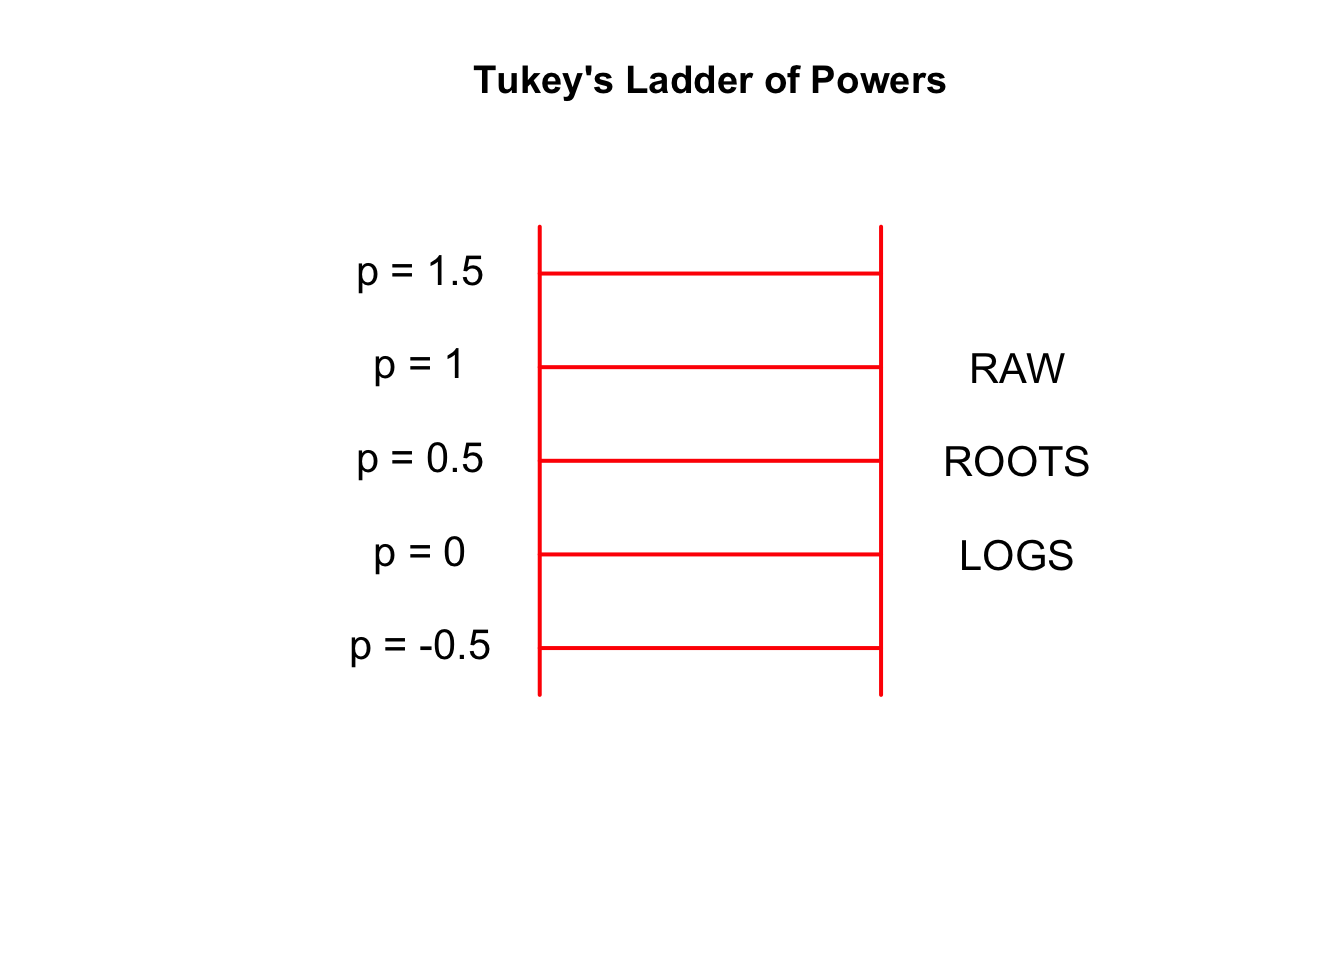
\includegraphics{Course-in-Exploratory-Data-Analysis_files/figure-latex/unnamed-chunk-39-1.pdf}

\begin{Shaded}
\begin{Highlighting}[]
\FunctionTok{spread\_level\_plot}\NormalTok{(beatles, New, album)}
\end{Highlighting}
\end{Shaded}

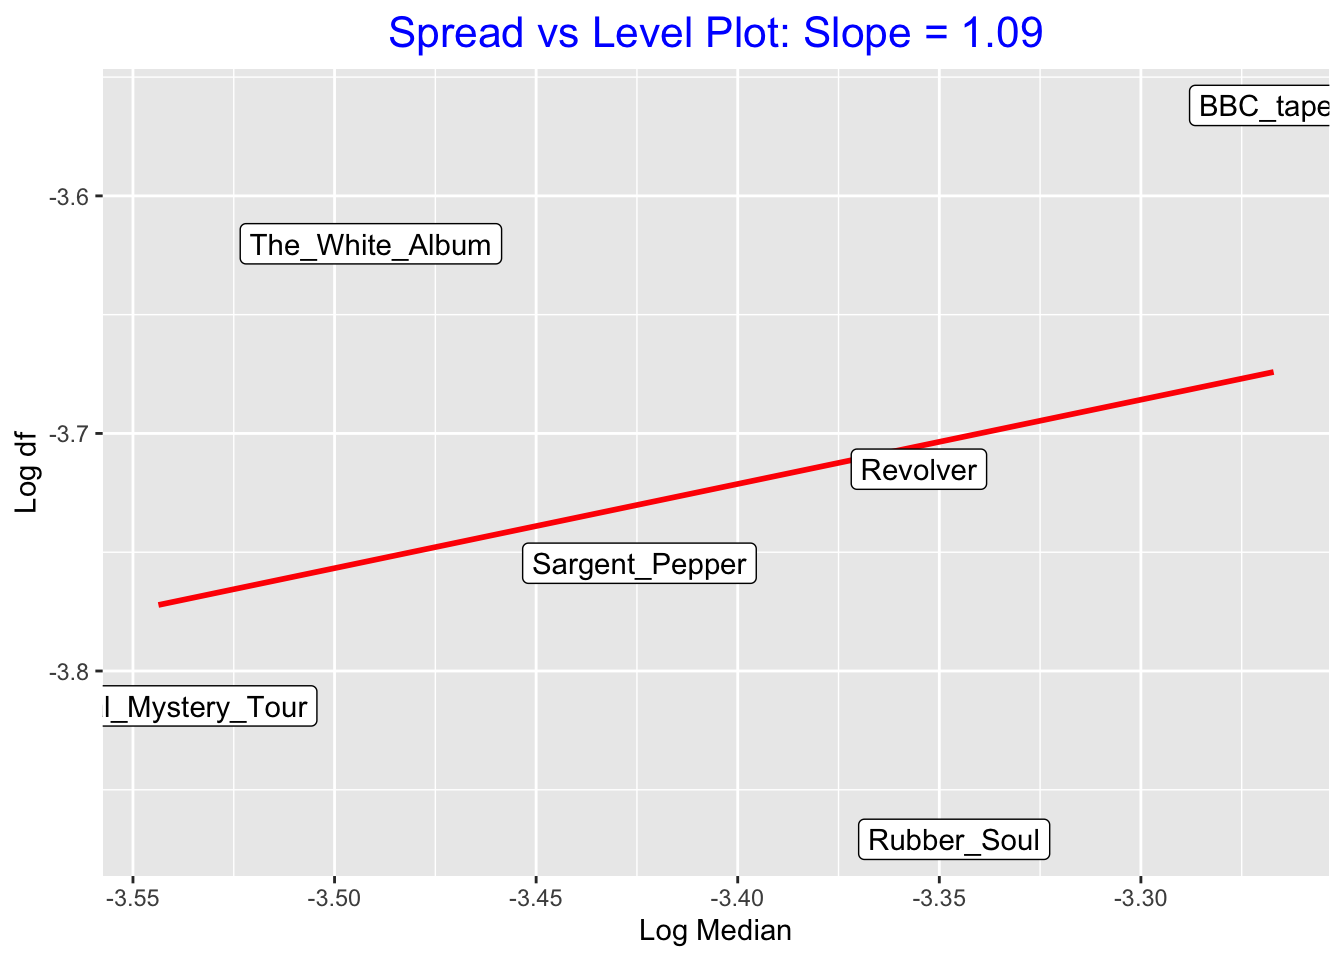
\includegraphics{Course-in-Exploratory-Data-Analysis_files/figure-latex/unnamed-chunk-39-2.pdf}

\begin{verbatim}
## # A tibble: 6 x 5
##   album                       M       df log.M log.df
##   <fct>                   <dbl>    <dbl> <dbl>  <dbl>
## 1 BBC_tapes            0.000541 0.000274 -3.27  -3.56
## 2 Magical_Mystery_Tour 0.000286 0.000153 -3.54  -3.81
## 3 Revolver             0.000442 0.000193 -3.36  -3.72
## 4 Rubber_Soul          0.000450 0.000135 -3.35  -3.87
## 5 Sargent_Pepper       0.000376 0.000176 -3.42  -3.75
## 6 The_White_Album      0.000323 0.000240 -3.49  -3.62
\end{verbatim}

Are we successful in this case in reducing the dependence between spread and level?

\begin{enumerate}
\def\labelenumi{\arabic{enumi}.}
\item
  First, look at the spread vs level plot for the reexpressed data \((time)^{-2}\). I don't see much of a relationship between \(\log M\) and \(\log d_F\) in this plot, suggesting that we have removed the trend between spread and level.
\item
  Next, look at the boxplot display of the reexpressed data -- we do see some differences in spreads between the batches. Are the batches of the reexpressed data more similar in spread than the batches of the raw data? Let's compare the spreads (\(d_F\)s) side by side.
\end{enumerate}

\begin{verbatim}
dF (raw)    dF (reexpressed)
38.00   0.287
69.00   0.176
35.50   0.227
25.25   0.147
50.50   0.183
74.00   0.272
\end{verbatim}

I see a slight improvement using this reexpression. The spreads of the raw data range from 25.25 to 74 -- the largest spread is 74/25.25 = 2.9 times the smallest. Looking at the reexpressed data, the spreads range from .147 to .287 -- the ratio is 2.0. Actually, this is a small improvement -- it probably doesn't make any sense in this case to reexpress the times.

\hypertarget{some-final-comments-about-spread-vs.-level-plots}{%
\section{Some final comments about spread vs.~level plots}\label{some-final-comments-about-spread-vs.-level-plots}}

\begin{enumerate}
\def\labelenumi{\arabic{enumi}.}
\item
  In practice, one chooses a power transformation where p is a multiple of one-half, like \(p = 1/2, p = 0, p = -1/2\) , etc. (We'll see soon that the \(p = 0\) power corresponds to taking a log.)
\item
  If the spread versus level plot suggests that you should take a power of p, you should check the effectiveness of the reexpression by
  o Constructing parallel boxplots of the data in the new scale
  o Making a spread versus level plot using the reexpressed data
\item
  Sometimes a certain form of reexpression is routinely made. For example, population counts are typically reexpressed using logs.
\end{enumerate}

\hypertarget{why-does-the-spread-vs.-level-plot-work}{%
\section{Why does the spread vs.~level plot work?}\label{why-does-the-spread-vs.-level-plot-work}}

Using some analytic work (not shown here), we can see when the spread versus level plot method is going to work. Generally the method will work when the fourth spread in the new scale is small relative to the median in the new scale.

Let's return to our music example. Here is the table of the medians and fourth-spreads of the reexpressed song lengths:

\begin{verbatim}
M   df
0.541   0.287
0.286   0.176
0.442   0.227
0.450   0.147
0.376   0.183
0.323   0.272
\end{verbatim}

If we divide the fourth-spreads by the corresponding medians, we get the values

\begin{verbatim}
  0.5305    0.6154    0.5136    0.3267    0.4867    0.8421
\end{verbatim}

These aren't really that small (I was hoping for ratios that were 0.2 or smaller). This explains why the spread vs level doesn't work very well for this example.

\hypertarget{transformations}{%
\chapter{Transformations}\label{transformations}}

In this lecture, we talk about transforming or reexpressing data. In the last two lectures, we have illustrated taking power transformations in order to reduce the dependence between spread and level. Here we talk more about the reasons why transformations can be helpful and more formally define the class of power transformations.

\hypertarget{why-do-we-rexpress-data}{%
\section{Why do we rexpress data?}\label{why-do-we-rexpress-data}}

Simply, we transform to make data easier to understand.

Here is a simple case in point. As you probably know, I'm a baseball fan and I'm interested in baseball data. Suppose we look at the number of home runs hit by all major league players in the year 1961. (I chose 1961 since it was a famous year for hitting home runs -- in particular, Roger Maris set the season record by hitting 61 home runs that season.) Below I have displayed these home run numbers using a histogram.

\begin{Shaded}
\begin{Highlighting}[]
\FunctionTok{library}\NormalTok{(LearnEDAfunctions)}
\FunctionTok{library}\NormalTok{(tidyverse)}
\FunctionTok{ggplot}\NormalTok{(homeruns}\FloatTok{.61}\NormalTok{, }\FunctionTok{aes}\NormalTok{(HR)) }\SpecialCharTok{+}
  \FunctionTok{geom\_histogram}\NormalTok{(}\AttributeTok{color =} \StringTok{"black"}\NormalTok{, }\AttributeTok{fill =} \StringTok{"white"}\NormalTok{)}
\end{Highlighting}
\end{Shaded}

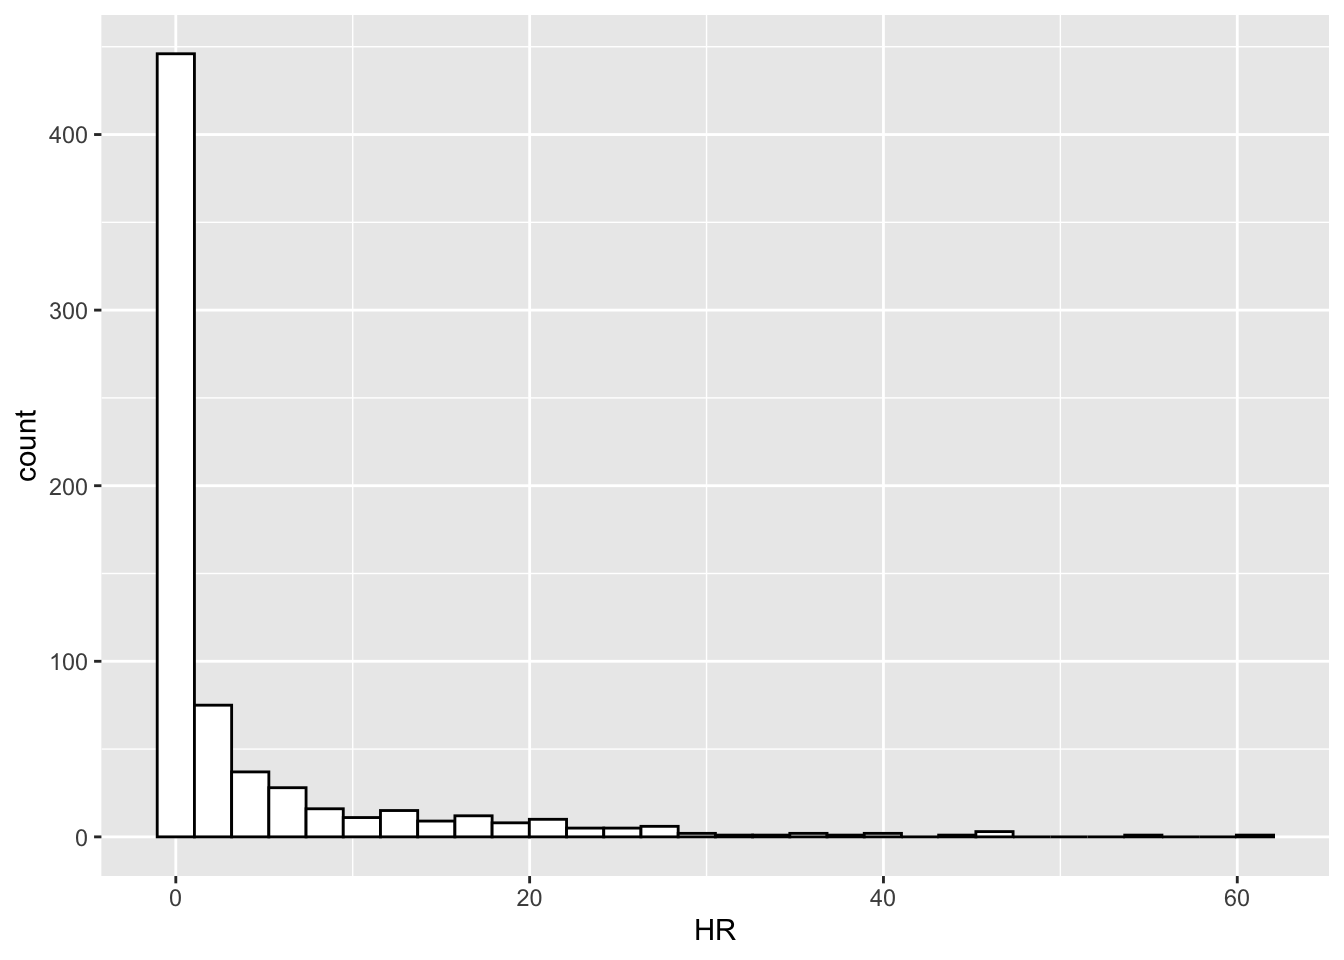
\includegraphics{Course-in-Exploratory-Data-Analysis_files/figure-latex/unnamed-chunk-40-1.pdf}

This data has strong right-skewness and is hard to analyze. All we can tell from the histogram is that most of the home run numbers are close to zero with a few large values. It is hard to distinguish the small values and I would have a hard time specifying an average home run number.

Generally, why is data hard to interpret?

\begin{itemize}
\item
  Strong asymmetry such as displayed in the above histogram.
\item
  A large number of outliers. These outliers can distort standard measures of average and spread, such as the mean and standard deviation. Also it creates difficulties just in graphing the data.
\item
  Batches with different averages and widely differing spreads. We saw this problem in the previous two lectures.
\item
  Large and systematic residuals after fitting a model. We'll talk more about patterns in residuals when we get to the plotting section of the class.
\end{itemize}

To make data easier to interpret, we want to choose a transformation which will change the shape of the data.

\hypertarget{the-shape-of-the-data}{%
\section{The shape of the data}\label{the-shape-of-the-data}}

The shape of the data is what you get when you draw a smooth curve over the histogram.

\begin{Shaded}
\begin{Highlighting}[]
\FunctionTok{ggplot}\NormalTok{(homeruns}\FloatTok{.61}\NormalTok{) }\SpecialCharTok{+}
       \FunctionTok{geom\_histogram}\NormalTok{(}\FunctionTok{aes}\NormalTok{(}\AttributeTok{x =}\NormalTok{ HR, }\AttributeTok{y =}\NormalTok{ ..density..)) }\SpecialCharTok{+}
       \FunctionTok{geom\_density}\NormalTok{(}\FunctionTok{aes}\NormalTok{(}\AttributeTok{x =}\NormalTok{ HR), }
              \AttributeTok{color =} \StringTok{"red"}\NormalTok{)}
\end{Highlighting}
\end{Shaded}

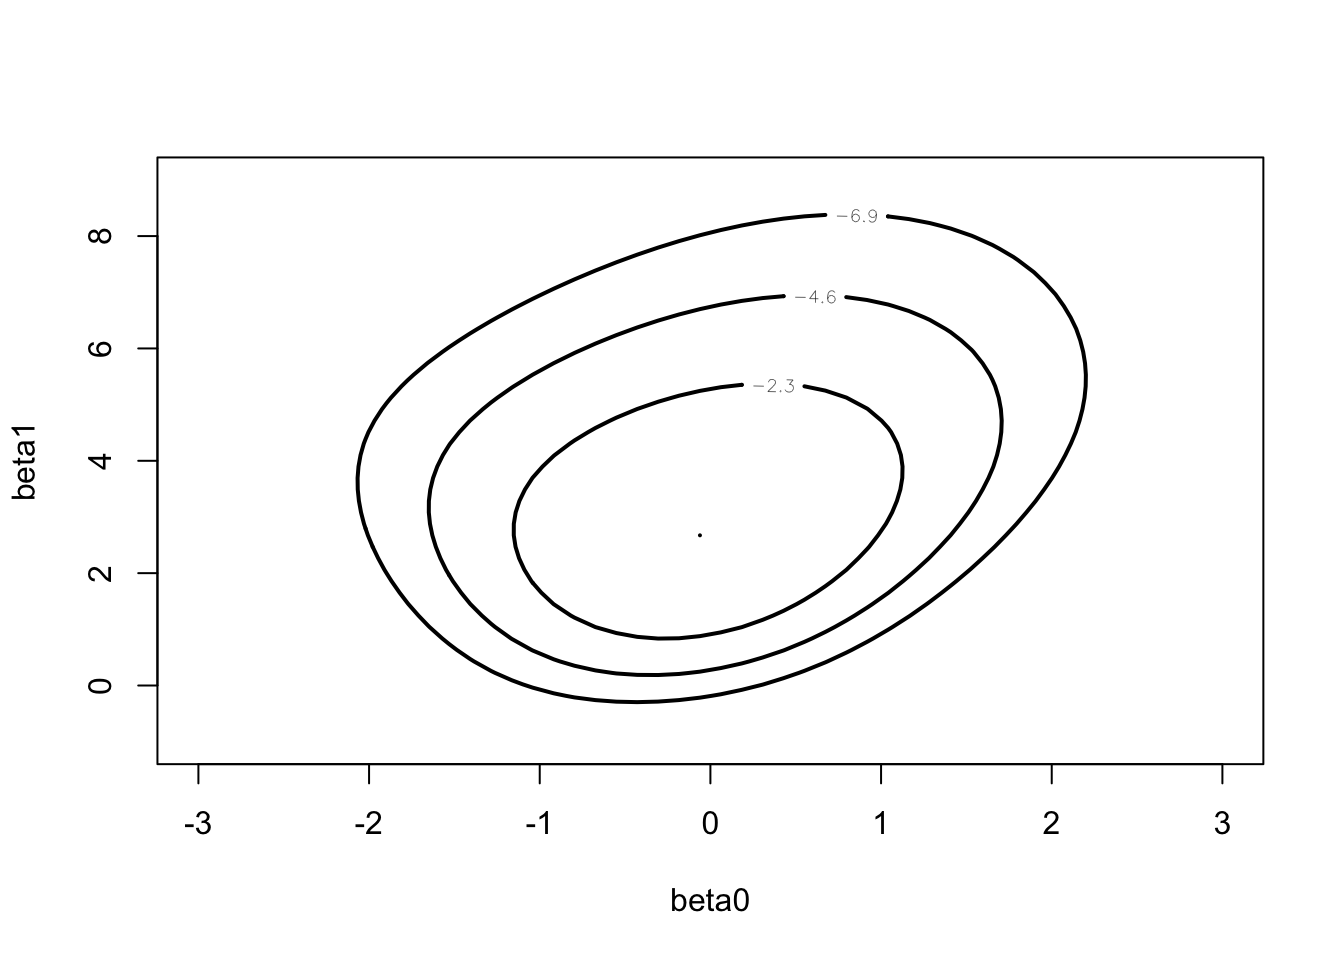
\includegraphics{Course-in-Exploratory-Data-Analysis_files/figure-latex/unnamed-chunk-41-1.pdf}

If we remove all of the labeling information and bars, we can focus on the shape:

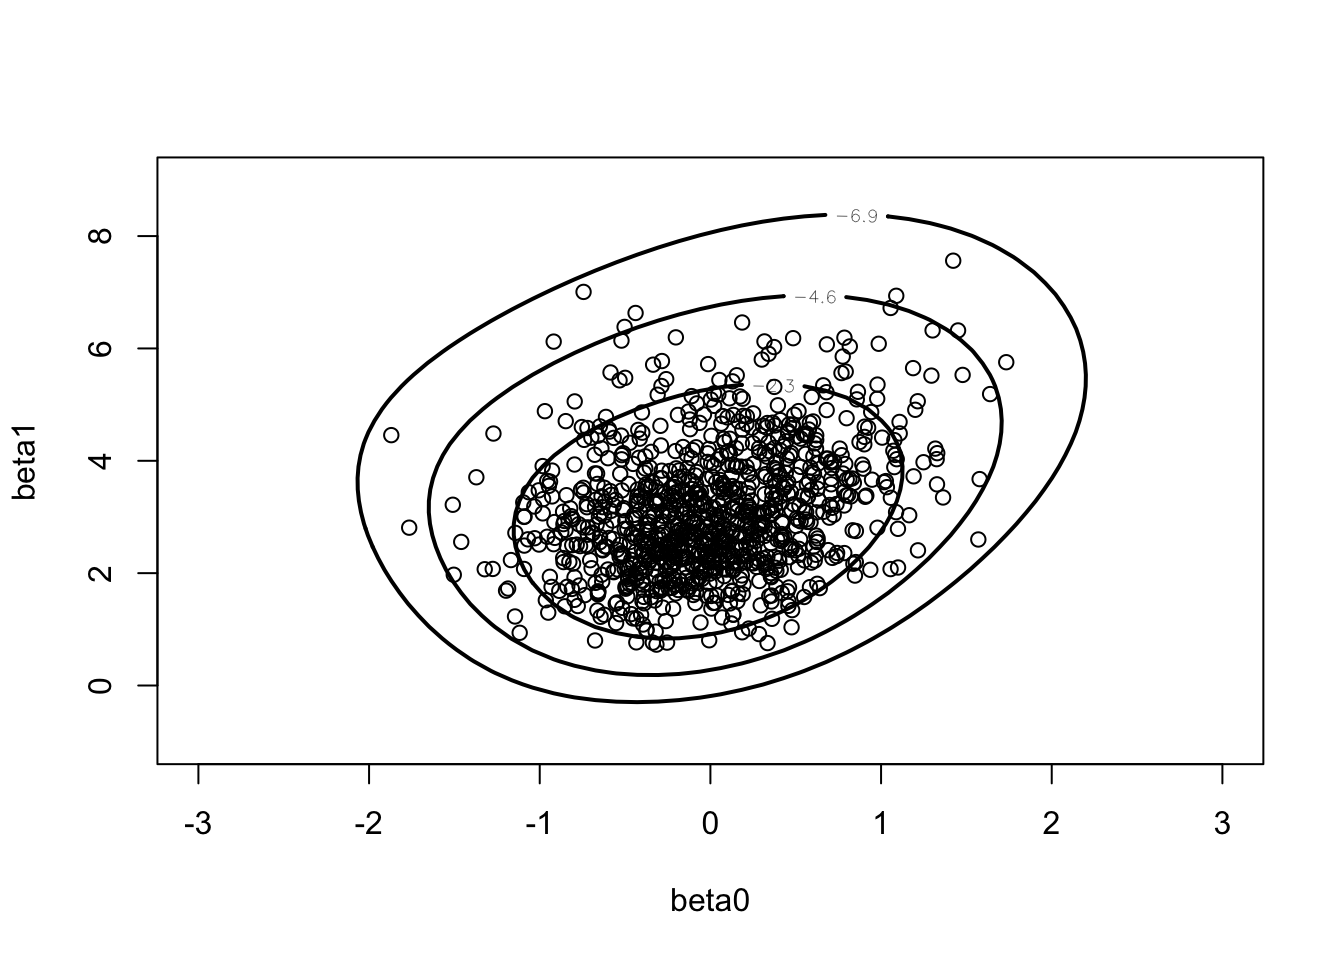
\includegraphics{Course-in-Exploratory-Data-Analysis_files/figure-latex/unnamed-chunk-42-1.pdf}

We are interested in finding a reexpression that can change this undesirable strong right-skewed shape.

\hypertarget{trivial-reexpressions}{%
\section{Trivial reexpressions}\label{trivial-reexpressions}}

There are some reexpressions that we could try that would change the values, but would have no impact on the shape of the distribution -- we call these trivial reexpressions. For example, in baseball a home run counts as four bases. We could reexpress home runs to bases:

\[
Bases = 4 (Home runs)
\]

If we constructed a histogram of all the bases numbers for all players, what would it look like? The shape would be identical to the right-skewed one shown above. In other words, multiplying a data by a positive constant will have no impact on the shape of the data. Similarly, it might be obvious that if we add any constant to the data, the shape of the data wouldn't change. To summarize, if \(X\) is our raw data and we reexpress \(X\) by the linear transformation
\[
Y = a X + b, \, {\rm where} \, a > 0,
\]
the shape of the \(Y\) data will be identical to the shape of the \(X\) data.

\hypertarget{nontrivial-expressions-the-power-family}{%
\section{Nontrivial expressions: the power family}\label{nontrivial-expressions-the-power-family}}

We are interested in finding reexpressions that can change the shape of the data so that it is easier to analyze. A convenient family of transformations is the power family. The basic form of this transformation is given by
\[
T_p(X) = X^p.
\]
If we choose \(p = 1\), then \(T_p(X) = X\), the raw data. If we choose any value \(p\) that isn't equal to 1, then will have a shape that is different from the raw data \(X\).

Let's illustrate this fact using our home run data. In the figure below, we show the raw data (\(p = 1\)) and power transformations using (\(p = .5\)) and (\(p = .001\)). We make one small adjustment to the basic power transformation to account for the large number of zeros in the data. We first change \(X\) to \(X + .5\) (add .5 to each observation), and then take powers of \(X + .5\).

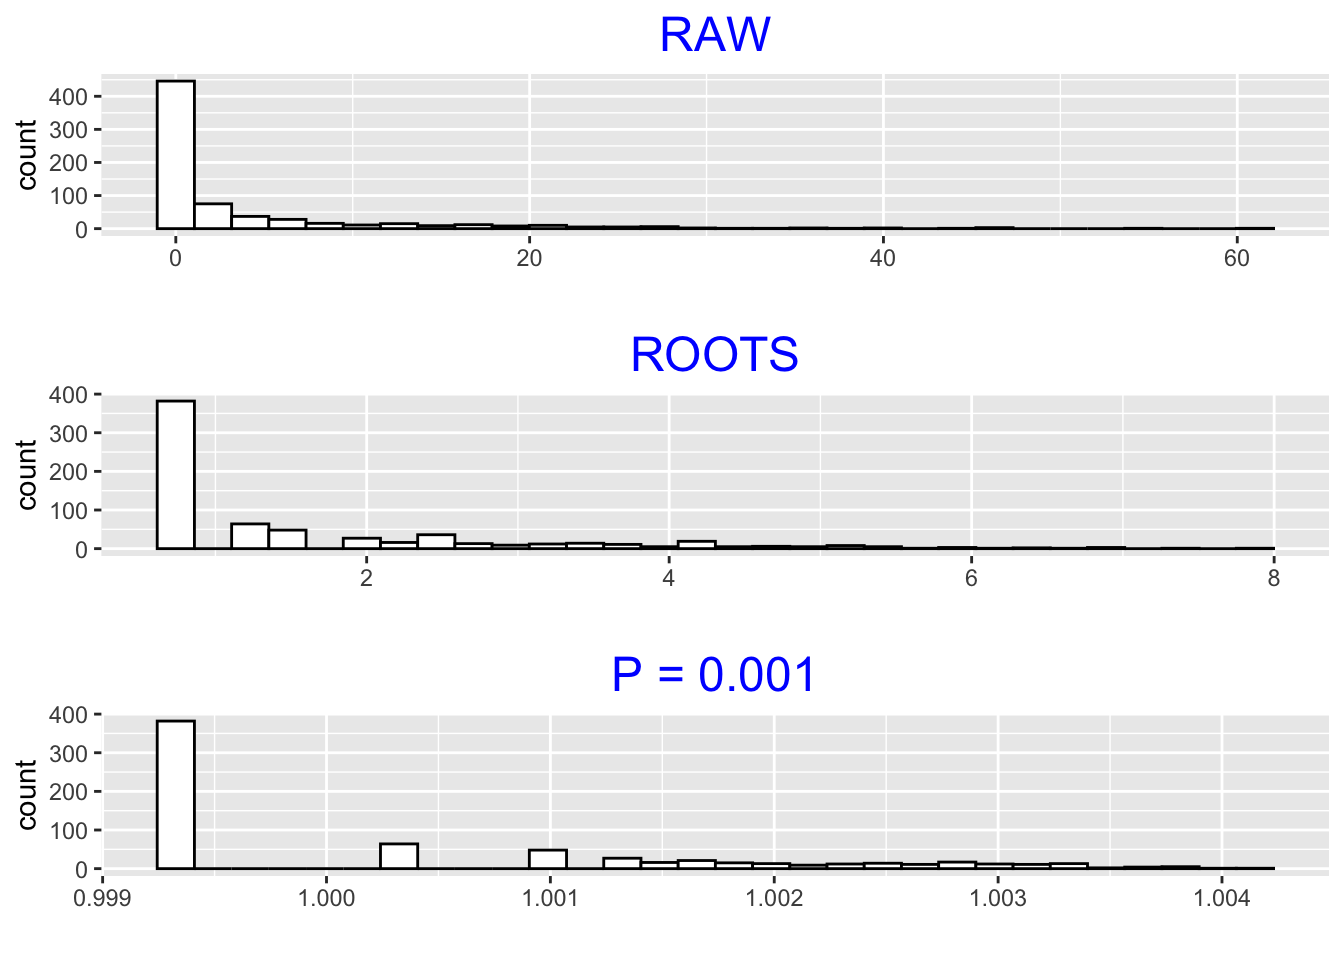
\includegraphics{Course-in-Exploratory-Data-Analysis_files/figure-latex/unnamed-chunk-43-1.pdf}

If we look from the raw data to the roots (\(p = .5\)) to the \(p\) = .001, we see distinctive changes in the data shape. The large amount of data close to zero in the raw plot gets squeezed out in the \(p = .5\) and \(p = .001\) graphs. In fact, in the \(p = .001\) plot, we are starting to see much more structure in the large data values.

\hypertarget{some-properties-of-the-power-family}{%
\section{Some properties of the power family}\label{some-properties-of-the-power-family}}

Above we presented the \texttt{basic\ form"\ of\ the\ power\ transformation.\ \ An\ alternative\ form\ of\ this\ power\ transformation\ is\ the}matched form'' --
\[
T_p(X) = \frac{X^p - 1}{p}.
\]
Suppose we graph this function (for fixed \(p\)) as a function of \(x\).

Note that for any value of the power \(p\),

\begin{itemize}
\tightlist
\item
  the graph goes through the point (1, 0) -- that is \(T_p(1) = 0\)
\item
  the derivative of the graph at \(x = 0\) is equal to 1 -- that is, \(T_p'(1) = 1\)
\end{itemize}

Below we have graphed the function \(T_p(x)\) for the powers \(p = 1.5, 1, .5, 0, -.5\).

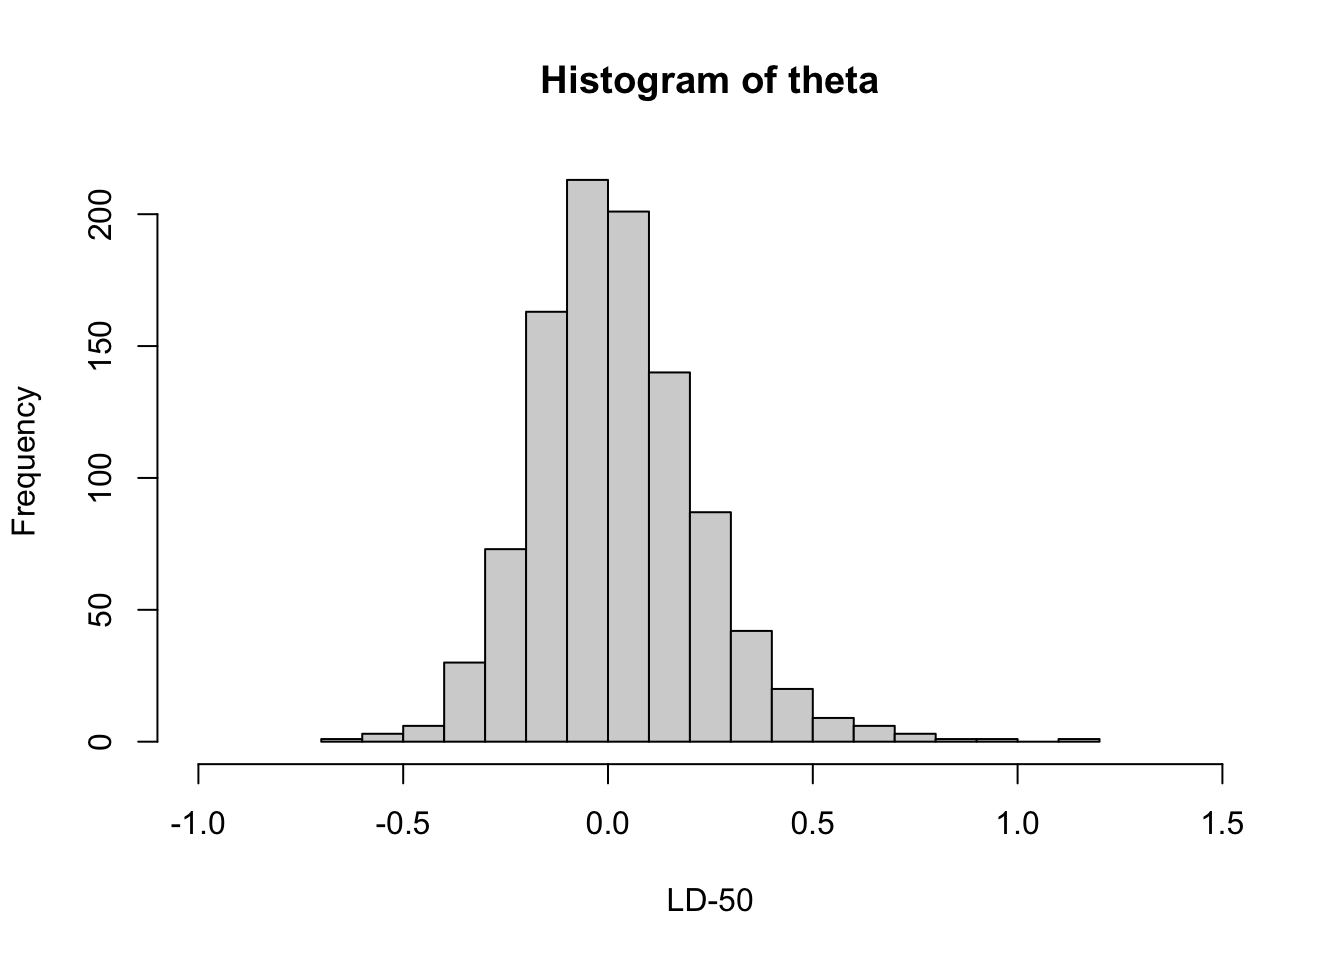
\includegraphics{Course-in-Exploratory-Data-Analysis_files/figure-latex/unnamed-chunk-44-1.pdf}

What do we notice in the graphs?

\begin{itemize}
\item
  we confirm that all of the graphs go through (1, 0) and have the same slope at that point
\item
  all of the curves are increasing in \(x\)
  (This is an important property -- when we apply this matched transformation to our raw data, we will preserve the order in the data.)
\item
  with respect to concavity
\item
  if \(p\) \textgreater{} 1, the graph is concave up
\item
  if \(p\) \textless{} 1, the graph is concave down
\item
  if \(p\) = 1, we have a linear function
\item
  as \(p\) moves away from 1, the curve becomes more curved, which means that the concavity increases
\end{itemize}

What impact does this concavity have on changing the shape of our data?

\begin{itemize}
\item
  If \(p\) \textgreater{} 1, then the graph is concave up, which means that the transformation will expand the scale more for large \(x\) than for small \(x\).
\item
  Similarly, if the power \(p < 1\) (graph is concave down), the transformation will expand the scale more for small \(x\) than for large \(x\).
\end{itemize}

Note that if \(p < 0\), the coefficient of \(x^p\) will be negative. This might seem odd (we don't usually have data with negative sign), but this is necessary to make all of these matched transformations increasing in \(x\).

\hypertarget{the-log-transformation}{%
\section{The log transformation}\label{the-log-transformation}}

The log transformation actually is a special case of a power transformation. Consider the matched form of the power family. Fix \(x\) and let the power \(p\) approach zero. Then it is a straightforward calculation to show that
\[
T_p(x) = \frac{x^p - 1}{p} \rightarrow ln(x),
\]
where \(\ln()\) is the natural log function. So a log function essentially is a power transformation for \(p = 0\).

Does it matter what type of log we take when we reexpress? No.~The only difference between log(base e) and log (base anything else) is a scalar multiple, which is a trivial reexpression. In this case, we will generally take log base 10. We do so for ease of interpretation and communication.

\hypertarget{ladders-of-powers}{%
\section{Ladders of powers}\label{ladders-of-powers}}

John Tukey used a ladder motif to describe different values \(p\) of the power transformation. We view the powers as rungs of a ladder.

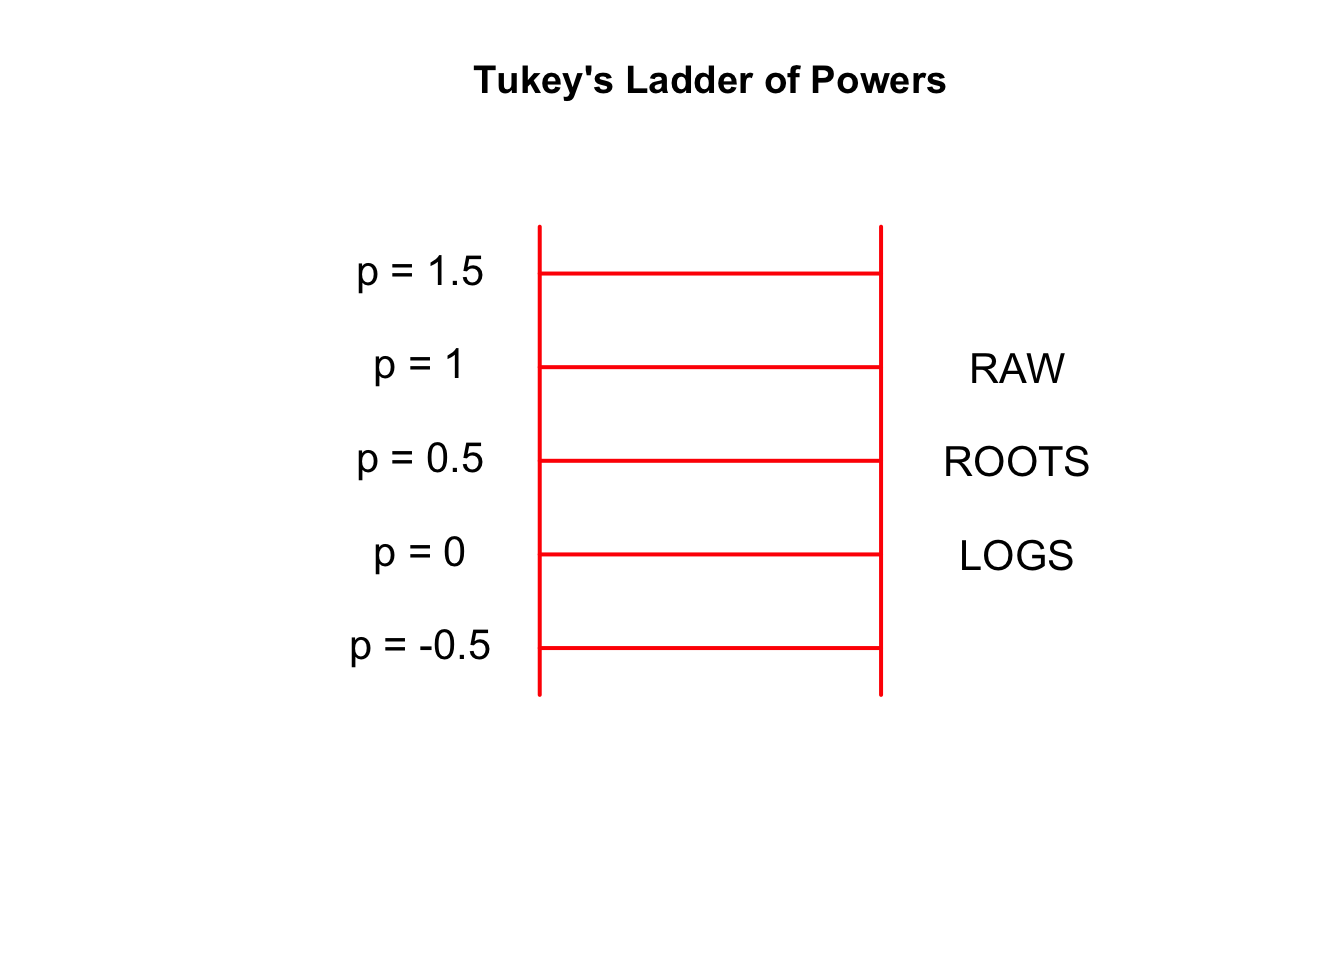
\includegraphics{Course-in-Exploratory-Data-Analysis_files/figure-latex/unnamed-chunk-45-1.pdf}

The raw data can be represented as a \(p = 1\) reexpression. Each move down the ladder (by a multiple of .5) is called one step and represents one unit change in the curvature of the transformation. If we wish to reexpress our data, we might change our data by taking roots, which is one step away from the raw data. If we wish to make a more drastic transformation, we might take another step, trying logs, which is the \(p = 0\) transformation.

In the next lecture, we'll get some experience taking power transformations with the objective of making a data set more symmetric.

\hypertarget{reexpressing-for-symmetry}{%
\chapter{Reexpressing for Symmetry}\label{reexpressing-for-symmetry}}

\hypertarget{data-for-the-day}{%
\section{Data for the day}\label{data-for-the-day}}

There is a great variation in the care of infants across different countries. One way of measuring the quality of care of newborns is by the infant mortality rate, which is defined to be the number who die for each 1000 births. The dataset \texttt{mortality.rate} in the \texttt{LearnEDA} package gives the mortality rates (years 2005 to 2010) for 62 countries (Afghanistan through Ghana). (Data comes from page 493 from the 2010 New York Times Almanac.) Part of the dataset is displayed below.

\begin{Shaded}
\begin{Highlighting}[]
\FunctionTok{library}\NormalTok{(LearnEDAfunctions)}
\FunctionTok{library}\NormalTok{(tidyverse)}
\FunctionTok{head}\NormalTok{(mortality.rates)}
\end{Highlighting}
\end{Shaded}

\begin{verbatim}
##       Country Rate
## 1 Afghanistan  157
## 2     Albania   16
## 3     Algeria   31
## 4      Angola  118
## 5   Argentina   13
## 6     Armenia   25
\end{verbatim}

Here is a stemplot of the raw data:

\begin{Shaded}
\begin{Highlighting}[]
\NormalTok{aplpack}\SpecialCharTok{::}\FunctionTok{stem.leaf}\NormalTok{(mortality.rates}\SpecialCharTok{$}\NormalTok{Rate)}
\end{Highlighting}
\end{Shaded}

\begin{verbatim}
## 1 | 2: represents 12
##  leaf unit: 1
##             n: 62
##   17     0 | 34444445556667899
##   26     1 | 000233679
##   (7)    2 | 0123356
##   29     3 | 01556
##   24     4 | 35568
##   19     5 | 14
##   17     6 | 27
##   15     7 | 3799
##   11     8 | 0557
##    7     9 | 8
##    6    10 | 06
##    4    11 | 38
##         12 | 
##    2    13 | 0
## HI: 157
\end{verbatim}

We see right-skewness in these data. Most of the mortality rates (corresponding to the more developed countries) are in the 0-30 range, and we notice several large rates (130, 157).

\hypertarget{why-is-this-data-hard-to-interpret}{%
\section{Why is this data hard to interpret?}\label{why-is-this-data-hard-to-interpret}}

When data is right or left skewed, then it is more difficult to analyze. Why?

\begin{itemize}
\tightlist
\item
  Most of the data is bunched up at one end of the distribution. This makes it hard to distinguish data values within the bunch.
\item
  The presence of outliers distorts the graphical display. Because there are gaps at the high end, only a small part of the display contains a majority of the data.
\item
  It is difficult to talk about an ``average'' value, since it is not well-defined. The median and mean will be different values.\\
\item
  It is harder to interpret a measure of spread like a standard deviation or fourth-spread when the data is skewed.
\end{itemize}

It is desirable to reexpress the data to make it more symmetric. We'll accomplish this by a suitable choice of power transformation.

\hypertarget{checking-for-symmetry-by-looking-at-midsummaries}{%
\section{Checking for symmetry by looking at midsummaries}\label{checking-for-symmetry-by-looking-at-midsummaries}}

In checking for symmetry, it is useful to have some tools for detecting symmetry of a batch of numbers. One useful method looks at the sequence of midsummaries.

First, a midsummary (or mid for short) is the average of the two letter values. The first midsummary is the median \(M\). The next midsummary is the average of the fourths -- we call this the midfourth:
\[
midfourth = \frac{F_U + F_L}{2}.
\]
Likewise, the mideighth is the average of the lower and upper eights, and so on. The R function \texttt{lval} from the \texttt{LearnEDAfunctions} package (illustrated here for the infant mortality data) shows the letter values and the corresponding mids:

\begin{Shaded}
\begin{Highlighting}[]
\NormalTok{(letter.values }\OtherTok{\textless{}{-}} \FunctionTok{lval}\NormalTok{(mortality.rates}\SpecialCharTok{$}\NormalTok{Rate))}
\end{Highlighting}
\end{Shaded}

\begin{verbatim}
##   depth lo    hi  mids spreads
## M  31.5 24  24.0 24.00     0.0
## H  16.0  9  67.0 38.00    58.0
## E   8.5  5  86.0 45.50    81.0
## D   4.5  4 109.5 56.75   105.5
## C   2.5  4 124.0 64.00   120.0
## B   1.0  3 157.0 80.00   154.0
\end{verbatim}

We can detect symmetry, or lack of symmetry, of a batch by looking at the sequence of midsummaries:

\begin{Shaded}
\begin{Highlighting}[]
\FunctionTok{select}\NormalTok{(letter.values, mids)}
\end{Highlighting}
\end{Shaded}

\begin{verbatim}
##    mids
## M 24.00
## H 38.00
## E 45.50
## D 56.75
## C 64.00
## B 80.00
\end{verbatim}

If this sequence

\begin{itemize}
\tightlist
\item
  is increasing (like it is here), then this indicates right skewness
\item
  is decreasing, we have left skewness
\item
  doesn't show any trend, then we have approximate symmetry
\end{itemize}

It is helpful to plot the midsummaries as a function of the letter value (Median is 1, Fourth is 2, etc). Clearly there is a positive trend in the plot, suggesting right skewness in the data.

\begin{Shaded}
\begin{Highlighting}[]
\NormalTok{letter.values }\SpecialCharTok{\%\textgreater{}\%} \FunctionTok{mutate}\NormalTok{(}\AttributeTok{LV =} \DecValTok{1}\SpecialCharTok{:}\DecValTok{6}\NormalTok{) }\SpecialCharTok{\%\textgreater{}\%} 
  \FunctionTok{ggplot}\NormalTok{(}\FunctionTok{aes}\NormalTok{(LV, mids)) }\SpecialCharTok{+}
  \FunctionTok{geom\_point}\NormalTok{() }\SpecialCharTok{+} \FunctionTok{ggtitle}\NormalTok{(}\StringTok{"Raw Data"}\NormalTok{)}
\end{Highlighting}
\end{Shaded}

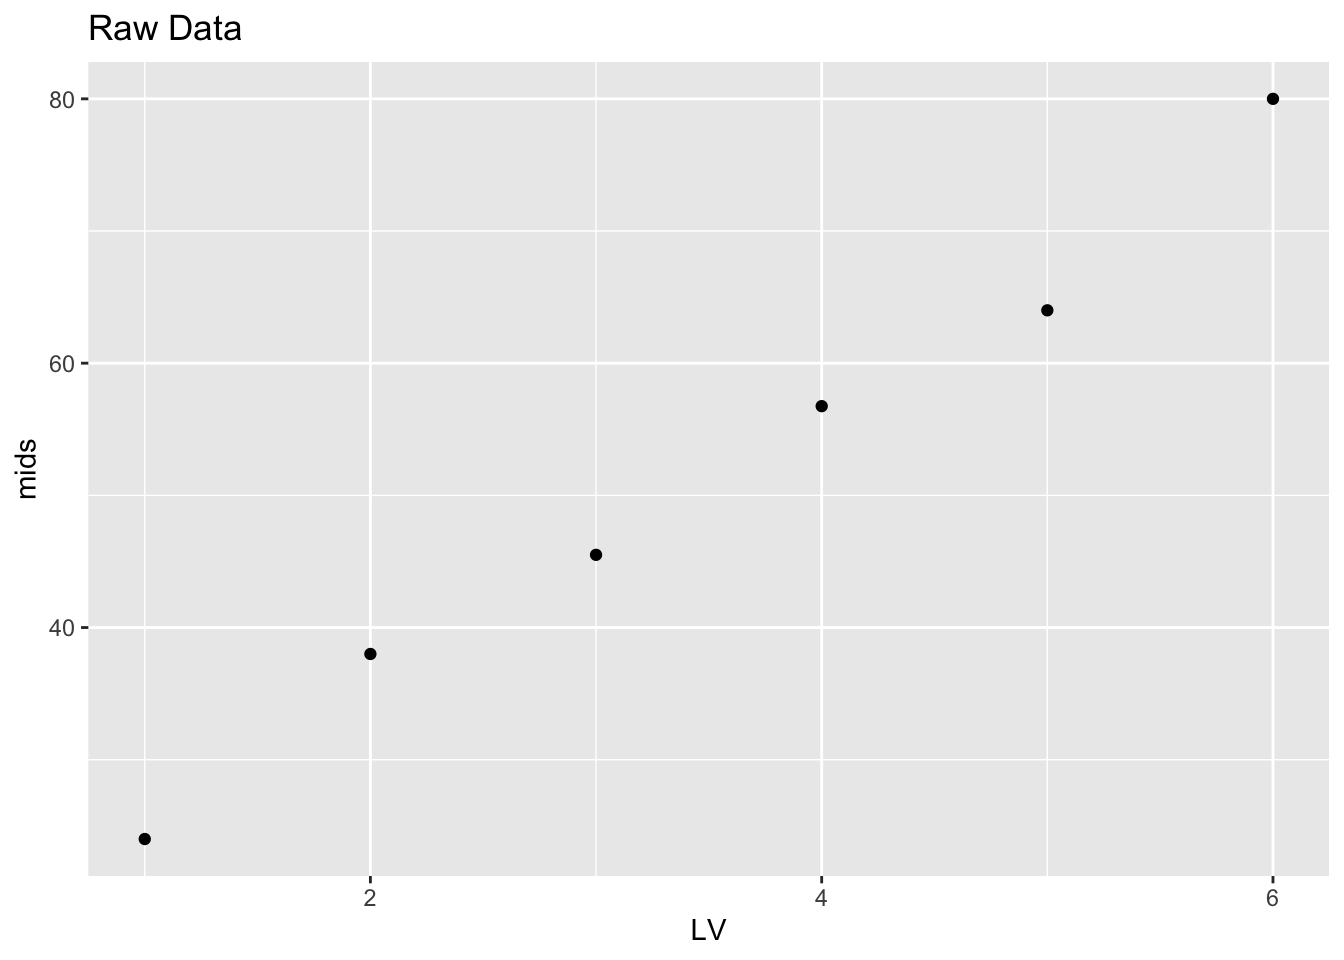
\includegraphics{Course-in-Exploratory-Data-Analysis_files/figure-latex/unnamed-chunk-50-1.pdf}

\hypertarget{reexpressing-to-achieve-approximate-symmetry}{%
\section{Reexpressing to achieve approximate symmetry}\label{reexpressing-to-achieve-approximate-symmetry}}

When we have skewness, then we move along the ladder of powers (of a power transformation) to look for a reexpression that will make the data set roughly symmetric. If we have right skewness (which is pretty common), then we move down the ladder of powers in our search for a good reexpression. Since the raw data is the \(p = 1\) transformation, we first take on step down on the ladder which corresponds to taking roots (\(p = 1/2\)).

We take roots of the data. Here is a stemplot, letter value display, and plot of the midsummaries for the roots:

\begin{Shaded}
\begin{Highlighting}[]
\NormalTok{roots }\OtherTok{\textless{}{-}} \FunctionTok{sqrt}\NormalTok{(mortality.rates}\SpecialCharTok{$}\NormalTok{Rate)}
\NormalTok{aplpack}\SpecialCharTok{::}\FunctionTok{stem.leaf}\NormalTok{(roots)}
\end{Highlighting}
\end{Shaded}

\begin{verbatim}
## 1 | 2: represents 1.2
##  leaf unit: 0.1
##             n: 62
##    1     1 | 7
##   15     2 | 00000022244468
##   23     3 | 00111466
##   (8)    4 | 01345677
##   (6)    5 | 004599
##   25     6 | 057779
##   19     7 | 138
##   16     8 | 157889
##   10     9 | 2238
##    6    10 | 0268
##    2    11 | 4
##    1    12 | 5
\end{verbatim}

\begin{Shaded}
\begin{Highlighting}[]
\NormalTok{(root.lv }\OtherTok{\textless{}{-}} \FunctionTok{lval}\NormalTok{(roots))}
\end{Highlighting}
\end{Shaded}

\begin{verbatim}
##   depth       lo        hi     mids   spreads
## M  31.5 4.897916  4.897916 4.897916  0.000000
## H  16.0 3.000000  8.185353 5.592676  5.185353
## E   8.5 2.236068  9.273462 5.754765  7.037394
## D   4.5 2.000000 10.462888 6.231444  8.462888
## C   2.5 2.000000 11.132267 6.566134  9.132267
## B   1.0 1.732051 12.529964 7.131007 10.797913
\end{verbatim}

\begin{Shaded}
\begin{Highlighting}[]
\NormalTok{root.lv }\SpecialCharTok{\%\textgreater{}\%} \FunctionTok{mutate}\NormalTok{(}\AttributeTok{LV =} \DecValTok{1}\SpecialCharTok{:}\DecValTok{6}\NormalTok{) }\SpecialCharTok{\%\textgreater{}\%} 
  \FunctionTok{ggplot}\NormalTok{(}\FunctionTok{aes}\NormalTok{(LV, mids)) }\SpecialCharTok{+}
  \FunctionTok{geom\_point}\NormalTok{() }\SpecialCharTok{+} \FunctionTok{ggtitle}\NormalTok{(}\StringTok{"Root Data"}\NormalTok{)}
\end{Highlighting}
\end{Shaded}

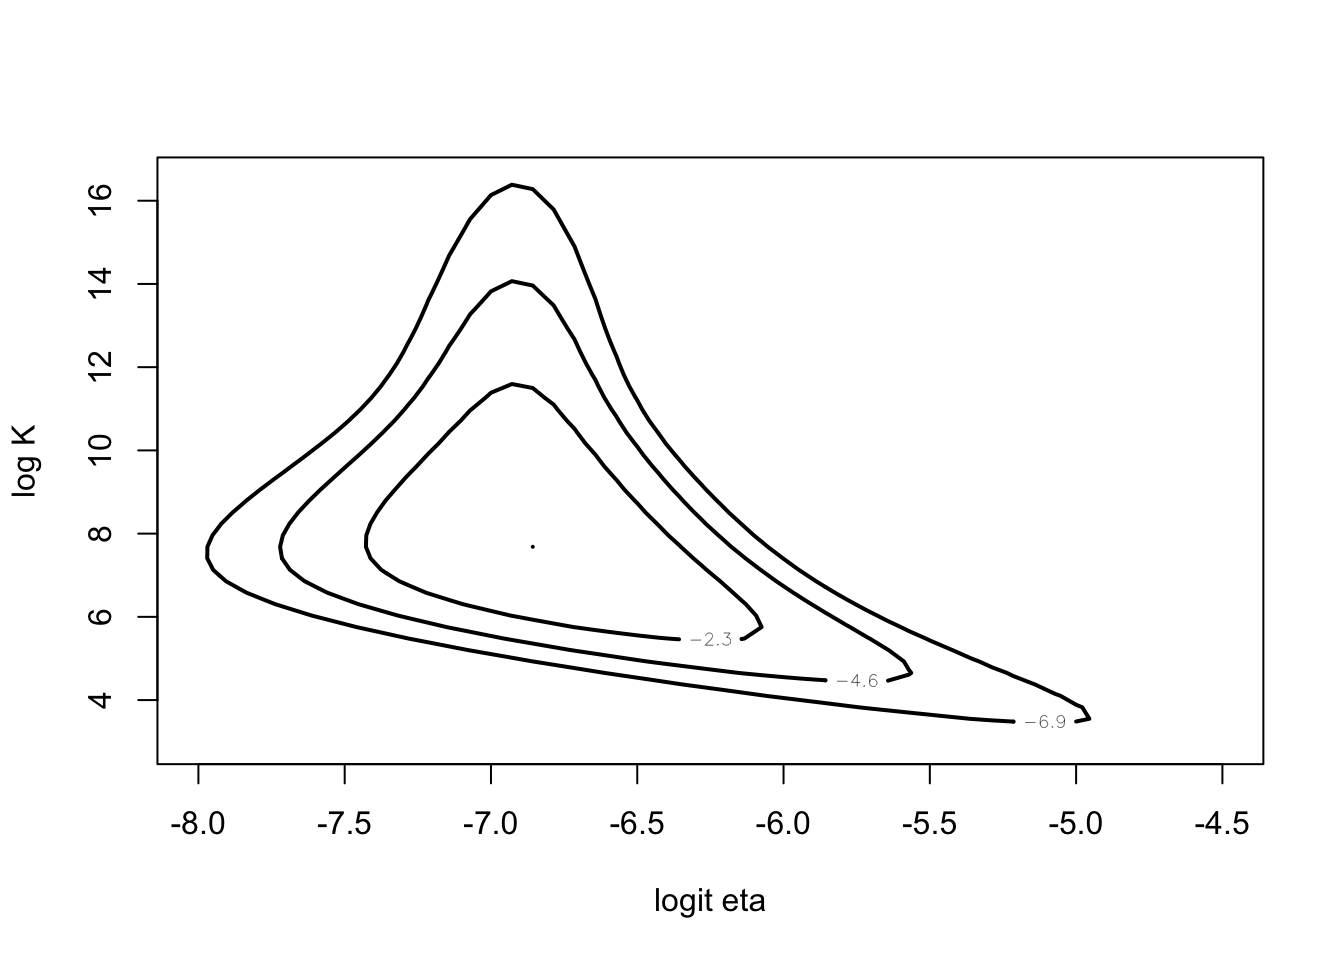
\includegraphics{Course-in-Exploratory-Data-Analysis_files/figure-latex/unnamed-chunk-51-1.pdf}

Things have improved. Comparing the stemplot of the roots with the stemplot of the raw mortality rates, the roots look less skewed, suggesting that we are moving in the right direction on the ladder of powers. But the data set is not symmetric -- this is confirmed by the plot of the midsummaries which shows a clear positive trend.

If we take another step down the ladder of powers, we arrive at logs \((p = 0)\). We display the stemplot, letter values, and plot of mids for the log mortality rates.

\begin{Shaded}
\begin{Highlighting}[]
\NormalTok{logs }\OtherTok{\textless{}{-}} \FunctionTok{log}\NormalTok{(mortality.rates}\SpecialCharTok{$}\NormalTok{Rate)}
\NormalTok{aplpack}\SpecialCharTok{::}\FunctionTok{stem.leaf}\NormalTok{(logs)}
\end{Highlighting}
\end{Shaded}

\begin{verbatim}
## 1 | 2: represents 1.2
##  leaf unit: 0.1
##             n: 62
##    7    1* | 0333333
##   14    1. | 6667779
##   21    2* | 0113334
##   27    2. | 557899
##   (8)   3* | 00112244
##   27    3. | 5557888899
##   17    4* | 1223333444
##    7    4. | 566778
##    1    5* | 0
\end{verbatim}

\begin{Shaded}
\begin{Highlighting}[]
\NormalTok{(logs.lv }\OtherTok{\textless{}{-}} \FunctionTok{lval}\NormalTok{(logs))}
\end{Highlighting}
\end{Shaded}

\begin{verbatim}
##   depth       lo       hi     mids  spreads
## M  31.5 3.177185 3.177185 3.177185 0.000000
## H  16.0 2.197225 4.204693 3.200959 2.007468
## E   8.5 1.609438 4.454280 3.031859 2.844842
## D   4.5 1.386294 4.695413 3.040854 3.309119
## C   2.5 1.386294 4.819110 3.102702 3.432815
## B   1.0 1.098612 5.056246 3.077429 3.957634
\end{verbatim}

\begin{Shaded}
\begin{Highlighting}[]
\NormalTok{logs.lv }\SpecialCharTok{\%\textgreater{}\%} \FunctionTok{mutate}\NormalTok{(}\AttributeTok{LV =} \DecValTok{1}\SpecialCharTok{:}\DecValTok{6}\NormalTok{) }\SpecialCharTok{\%\textgreater{}\%} 
  \FunctionTok{ggplot}\NormalTok{(}\FunctionTok{aes}\NormalTok{(LV, mids)) }\SpecialCharTok{+}
  \FunctionTok{geom\_point}\NormalTok{() }\SpecialCharTok{+} \FunctionTok{ggtitle}\NormalTok{(}\StringTok{"Log Data"}\NormalTok{)}
\end{Highlighting}
\end{Shaded}

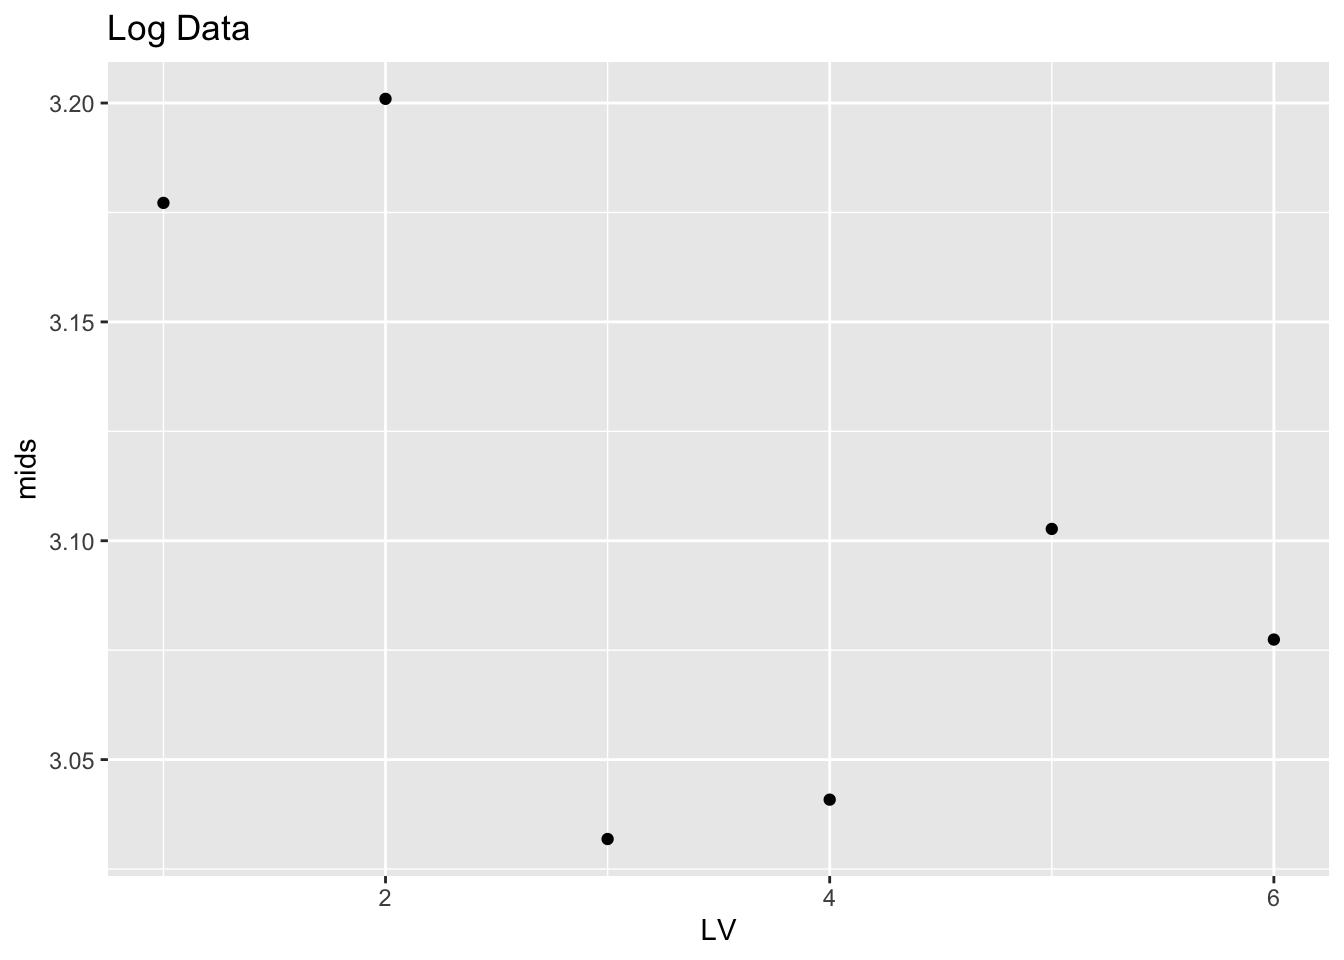
\includegraphics{Course-in-Exploratory-Data-Analysis_files/figure-latex/unnamed-chunk-52-1.pdf}

Things look a bit better. The stemplot looks pretty symmetric to me. Looking at the plot of the mids, there is a decreasing trend for the first three points, and then the plot looks pretty constant. This means that there is some skewness in the middle portion of the logs, but there is little skewness in the tails (the tails are the extreme portions of the data).

If logs are a good reexpression, then it wouldn't make any sense to go further down the ladder of powers. But let's check and try taking a \(p = -1/2\) rexpression which corresponds to reciprocal roots (\(1 / \sqrt{mortality \, rate}\) ). Actually we take the reexpression
\[
- \frac{1}{\sqrt{mortality \, rate}}.
\]
We do this since we want all of our power transformations to be increasing functions of our raw data.

Below we show the stemplot, the letter-value display, and the graph of the mids for the reciprocal roots.

\begin{Shaded}
\begin{Highlighting}[]
\NormalTok{recroots }\OtherTok{\textless{}{-}} \SpecialCharTok{{-}} \DecValTok{1} \SpecialCharTok{/} \FunctionTok{sqrt}\NormalTok{(mortality.rates}\SpecialCharTok{$}\NormalTok{Rate)}
\NormalTok{aplpack}\SpecialCharTok{::}\FunctionTok{stem.leaf}\NormalTok{(recroots)}
\end{Highlighting}
\end{Shaded}

\begin{verbatim}
## 1 | 2: represents 0.12
##  leaf unit: 0.01
##             n: 62
##    1    -5. | 7
##    7    -5* | 000000
##         -4. | 
##   13    -4* | 444000
##   15    -3. | 75
##   20    -3* | 33111
##   24    -2. | 8775
##   (8)   -2* | 42211000
##   30    -1. | 9876665
##   23    -1* | 444443221111100000
##    5    -0. | 99987
\end{verbatim}

\begin{Shaded}
\begin{Highlighting}[]
\NormalTok{(recroots.lv }\OtherTok{\textless{}{-}} \FunctionTok{lval}\NormalTok{(recroots))}
\end{Highlighting}
\end{Shaded}

\begin{verbatim}
##   depth         lo          hi       mids   spreads
## M  31.5 -0.2042572 -0.20425721 -0.2042572 0.0000000
## H  16.0 -0.3333333 -0.12216944 -0.2277514 0.2111639
## E   8.5 -0.4472136 -0.10783824 -0.2775259 0.3393754
## D   4.5 -0.5000000 -0.09560034 -0.2978002 0.4043997
## C   2.5 -0.5000000 -0.08988163 -0.2949408 0.4101184
## B   1.0 -0.5773503 -0.07980869 -0.3285795 0.4975416
\end{verbatim}

\begin{Shaded}
\begin{Highlighting}[]
\NormalTok{recroots.lv }\SpecialCharTok{\%\textgreater{}\%} \FunctionTok{mutate}\NormalTok{(}\AttributeTok{LV =} \DecValTok{1}\SpecialCharTok{:}\DecValTok{6}\NormalTok{) }\SpecialCharTok{\%\textgreater{}\%} 
  \FunctionTok{ggplot}\NormalTok{(}\FunctionTok{aes}\NormalTok{(LV, mids)) }\SpecialCharTok{+}
  \FunctionTok{geom\_point}\NormalTok{() }\SpecialCharTok{+} \FunctionTok{ggtitle}\NormalTok{(}\StringTok{"Reciprocal Roots"}\NormalTok{)}
\end{Highlighting}
\end{Shaded}

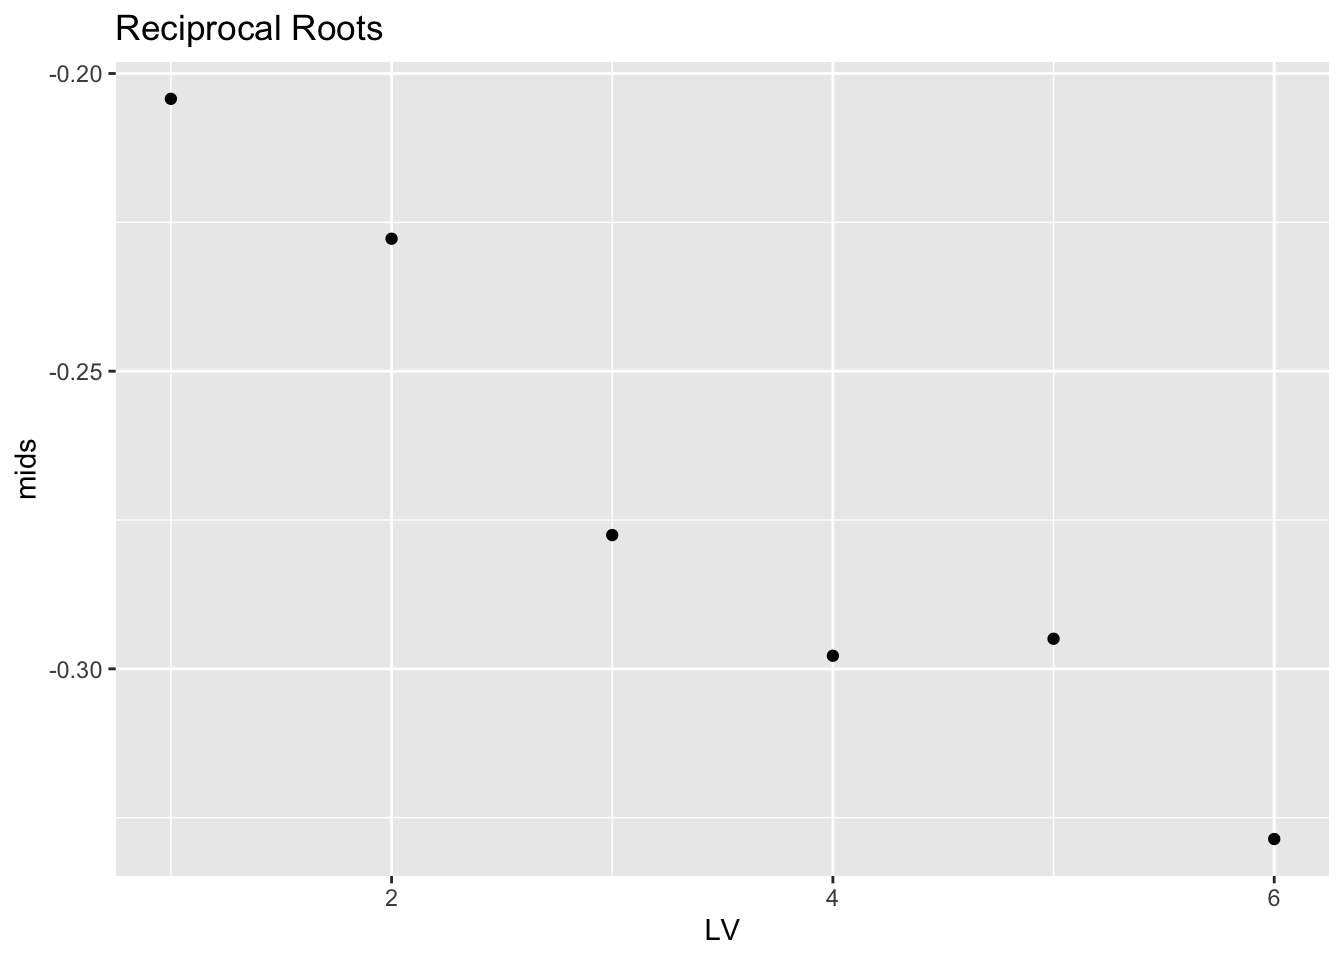
\includegraphics{Course-in-Exploratory-Data-Analysis_files/figure-latex/unnamed-chunk-53-1.pdf}

Looking at the stemplot, the distribution of the reciprocal roots looks left-skewed. There is a negative trend in the midsummaries that confirms this left-skewness. (Actually the graph of the mids of the reciprocal roots looks similar to the graph of the mids of the logs. But I'm combining all of the information that we get from a visual scan of the stemplot and the midsummaries.)

So this analysis suggests that we should take the log of the mortality rates to achieve approximate symmetry.

\hypertarget{hinkleys-quick-method}{%
\section{Hinkley's quick method}\label{hinkleys-quick-method}}

David Hinkley suggested a simple measure of asymmetry of a batch. This measure can be used together with the family of power transformations to suggest an appropriate reexpression.

He suggested looking at the statistic
\[
d = \frac{\bar X - M}{measure \, of \, scale},
\]
where \(\bar X\) is the mean, \(M\) is the median, and the denominator is any measure of scale of the batch. In the following, we will use the fourth-spread as our scale measure.

To interpret d \ldots{}

\begin{itemize}
\tightlist
\item
  if d \textgreater{} 0, this indicates that the mean is larger than the median which reflects right-skewness of the batch
\item
  if d \textless{} 0, this indicates left-skewness
\item
  if d is approximately 0, then the batch appears roughly symmetric
\end{itemize}

For our batch of mortality rates, we can compute
\[
 \bar X = 39.80645, M = 24,  d_F = F_U - F_L = 67 ??? 9 = 58
\]
\[
d = \frac{39.80645 - 24}{58} = 0.2725,
\]
which indicates right-skewness in the batch.

As before, we move down the ladder of powers to suggest possible reexpressions. We use Hinkley's statistic to measure the skewness in the reexpressed batch. We choose the value of the power p so that the value of the skewness measure d is approximately equal to 0.

Using the \texttt{hinkley} function, we compute Hinkley's measure for the roots, logs, and reciprocal roots.

\begin{Shaded}
\begin{Highlighting}[]
\FunctionTok{hinkley}\NormalTok{(roots)}
\end{Highlighting}
\end{Shaded}

\begin{verbatim}
##         h 
## 0.1332907
\end{verbatim}

\begin{Shaded}
\begin{Highlighting}[]
\FunctionTok{hinkley}\NormalTok{(logs)}
\end{Highlighting}
\end{Shaded}

\begin{verbatim}
##           h 
## -0.02235429
\end{verbatim}

\begin{Shaded}
\begin{Highlighting}[]
\FunctionTok{hinkley}\NormalTok{(recroots)}
\end{Highlighting}
\end{Shaded}

\begin{verbatim}
##          h 
## -0.1950111
\end{verbatim}

Looking at the values of d, the ``correct'' reexpression appears to be between \(p = .5\) (roots) and \(p = 0\) (logs), although the value closest to 0 corresponds to the log reexpression.

In practice, one uses Hinkley's method together with other methods such as the midsummary approach to assess symmetry and find an appropriate choice of power transformation.

\hypertarget{reexpressing-for-symmetry-ii}{%
\chapter{Reexpressing for Symmetry II}\label{reexpressing-for-symmetry-ii}}

\hypertarget{data-for-the-day-1}{%
\section{Data for the day}\label{data-for-the-day-1}}

Where are the farms in the United States? The 2001 New York Times Almanac gives the number of farms (in 1000's) for each of the 50 states in 1999 -- the data is shown below. We will use this example to illustrate methods for determining the symmetry of a batch and to decide on appropriate reexpressions to make the batch more symmetric.

The dataset \texttt{farms} in the \texttt{LearnEDA} package contains this data. The first few rows are displayed below.

\begin{Shaded}
\begin{Highlighting}[]
\FunctionTok{library}\NormalTok{(LearnEDAfunctions)}
\FunctionTok{head}\NormalTok{(farms)}
\end{Highlighting}
\end{Shaded}

\begin{verbatim}
##   state count
## 1    Al    48
## 2   Als     1
## 3    Ar     8
## 4   Ark    49
## 5    Ca    89
## 6   Col    29
\end{verbatim}

Here is a stemplot of the data.

\begin{Shaded}
\begin{Highlighting}[]
\NormalTok{aplpack}\SpecialCharTok{::}\FunctionTok{stem.leaf}\NormalTok{(farms}\SpecialCharTok{$}\NormalTok{count, }
                   \AttributeTok{unit=}\DecValTok{10}\NormalTok{, }\AttributeTok{m=}\DecValTok{5}\NormalTok{, }\AttributeTok{trim.outliers=}\ConstantTok{FALSE}\NormalTok{)}
\end{Highlighting}
\end{Shaded}

\begin{verbatim}
## 1 | 2: represents 120
##  leaf unit: 10
##             n: 50
##    16    0* | 0000000000001111
##    (9)    t | 222223333
##   (12)    f | 444444555555
##    13     s | 6677
##     9    0. | 8888999
##     2    1* | 1
##           t | 
##           f | 
##           s | 
##          1. | 
##          2* | 
##     1     t | 2
\end{verbatim}

What do we see? Obviously we note the big outlier at 22 -- looking at the data, we see that this corresponds to the number of farms in Texas. Otherwise, we see some right skewness in the data. Next we look at the sequence of midsummaries shown in the letter value display below.

\begin{Shaded}
\begin{Highlighting}[]
\FunctionTok{lval}\NormalTok{(farms}\SpecialCharTok{$}\NormalTok{count)}
\end{Highlighting}
\end{Shaded}

\begin{verbatim}
##   depth   lo    hi  mids spreads
## M  25.5 39.5  39.5  39.5       0
## H  13.0 10.0  65.0  37.5      55
## E   7.0  6.0  84.0  45.0      78
## D   4.0  3.0  91.0  47.0      88
## C   2.5  2.0 104.0  53.0     102
## B   1.0  1.0 227.0 114.0     226
\end{verbatim}

The median (39.5) is larger than the mid-fourth (37.5) -- this indicates some left-skewness in the middle half of the data. Then the midsummaries increase from the mid-fourth to the mid-extremes -- this tells us that the outside half of the data is right-skewed.

\hypertarget{symmetry-plot}{%
\section{Symmetry plot}\label{symmetry-plot}}

We now introduce a new plot to learn about the symmetry of a batch -- not surprisingly, this is called a symmetry plot.

To make a symmetry plot \ldots{}

\begin{itemize}
\tightlist
\item
  First order the n data values -- call the ordered values \(y_{(1)}, ..., y_{(n)}\).
\item
  If \(M\) denotes the median then you plot the points
  \[
  u_i = y_{(n+1-i)} - M \, \, ({\rm vertical})
  \]
  against
  \[
  v_i = M - y_{(i)} \, \, ({\rm horizontal})
  \]
  for \(i = 1, ???, n/2\) (or \((n+1)/2\) if \(n\) is odd).
\item
  Add the line u = v to the graph.
\end{itemize}

Here is the symmetry plot for the farm numbers. Here we have 50 numbers, so we will plotting 25 \((u, v)\) points.

\begin{Shaded}
\begin{Highlighting}[]
\FunctionTok{symplot}\NormalTok{(farms}\SpecialCharTok{$}\NormalTok{count)}
\end{Highlighting}
\end{Shaded}

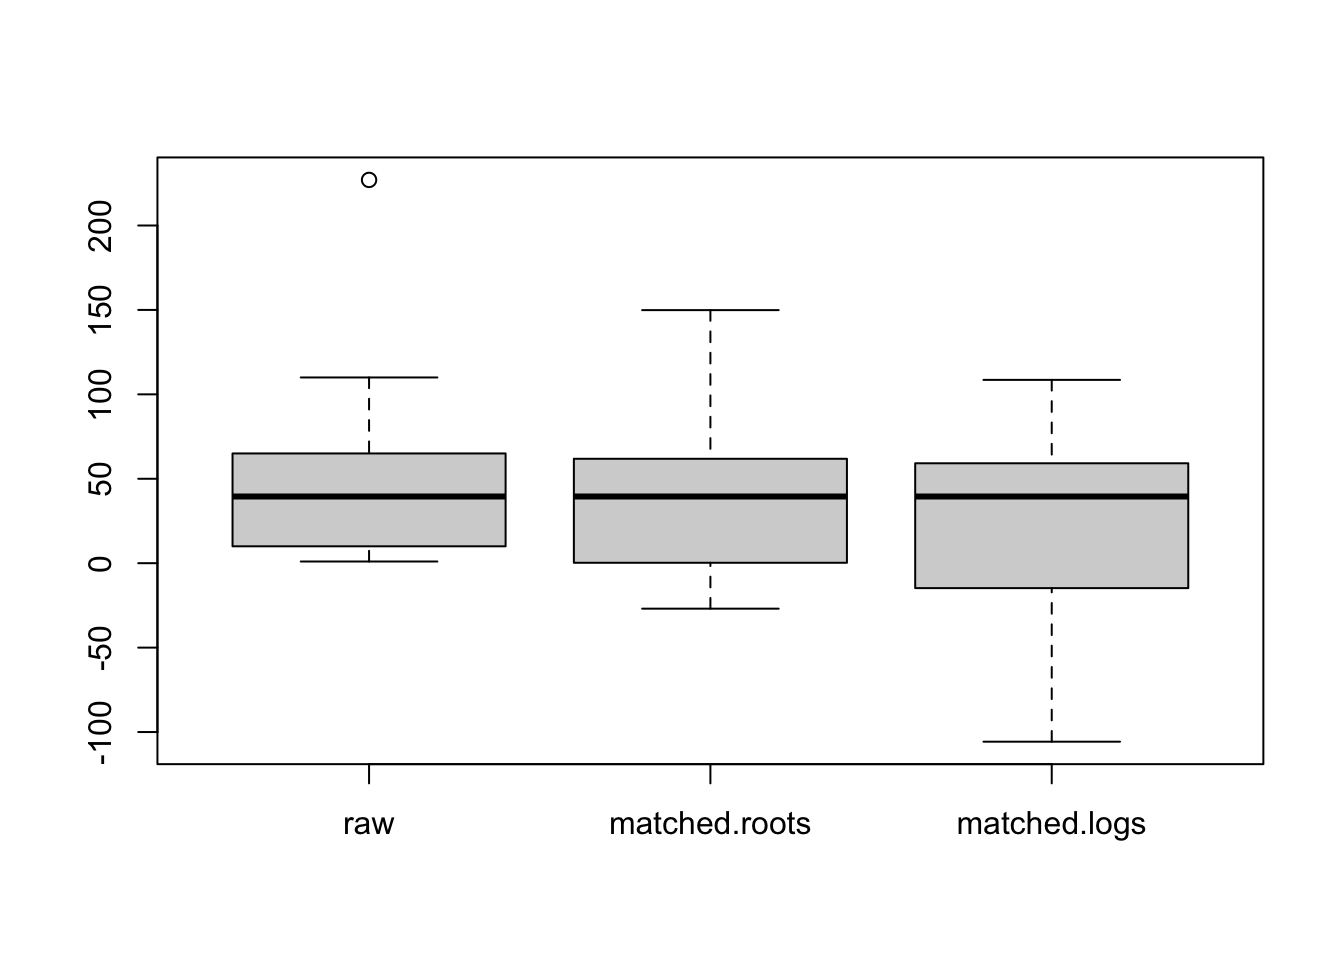
\includegraphics{Course-in-Exploratory-Data-Analysis_files/figure-latex/unnamed-chunk-58-1.pdf}

How do you interpret a symmetry plot? Some guidelines follow:

\begin{enumerate}
\def\labelenumi{\arabic{enumi}.}
\item
  If the points fall close to the line u = v, then the data is nearly symmetric.
\item
  If the data is left-skewed, then the points fall below the line as follows:
\item
  Likewise, if the data is right-skewed, the points fall above the line.
\item
  The plot is nondecreasing -- the points close to the origin correspond to values of the data close to the median M and the point on the far right correspond to the extremes.
\end{enumerate}

Let's return to the symmetry plot for the farm numbers.

If we look from left to right, we first see a number of point under the line \(u = v\), and then we see points above the line. This tells us that there is left-skewness in the middle of the batch and right skewness in the tail portion of the batch. These statements are consistent with what we saw in the sequence of midsummaries.

To remove the right-skewness that we see, we go down the ladder of powers and try power transformations \(p\) that are smaller than \(p = 1\).

\hypertarget{roots-and-logs}{%
\section{Roots and logs}\label{roots-and-logs}}

We first try roots (\(p = .5\)). Below, we show a stemplot, the letter value display and the symmetry plot.

\begin{Shaded}
\begin{Highlighting}[]
\NormalTok{roots }\OtherTok{\textless{}{-}} \FunctionTok{sqrt}\NormalTok{(farms}\SpecialCharTok{$}\NormalTok{count)}
\NormalTok{aplpack}\SpecialCharTok{::}\FunctionTok{stem.leaf}\NormalTok{(roots)}
\end{Highlighting}
\end{Shaded}

\begin{verbatim}
## 1 | 2: represents 1.2
##  leaf unit: 0.1
##             n: 50
##    5     1 | 00777
##   11     2 | 044668
##   14     3 | 014
##   17     4 | 005
##   24     5 | 0023457
##   (6)    6 | 234579
##   20     7 | 0002466
##   13     8 | 00889
##    8     9 | 014558
##    2    10 | 4
##         11 | 
##         12 | 
##         13 | 
##         14 | 
##    1    15 | 0
\end{verbatim}

\begin{Shaded}
\begin{Highlighting}[]
\FunctionTok{symplot}\NormalTok{(roots)}
\end{Highlighting}
\end{Shaded}

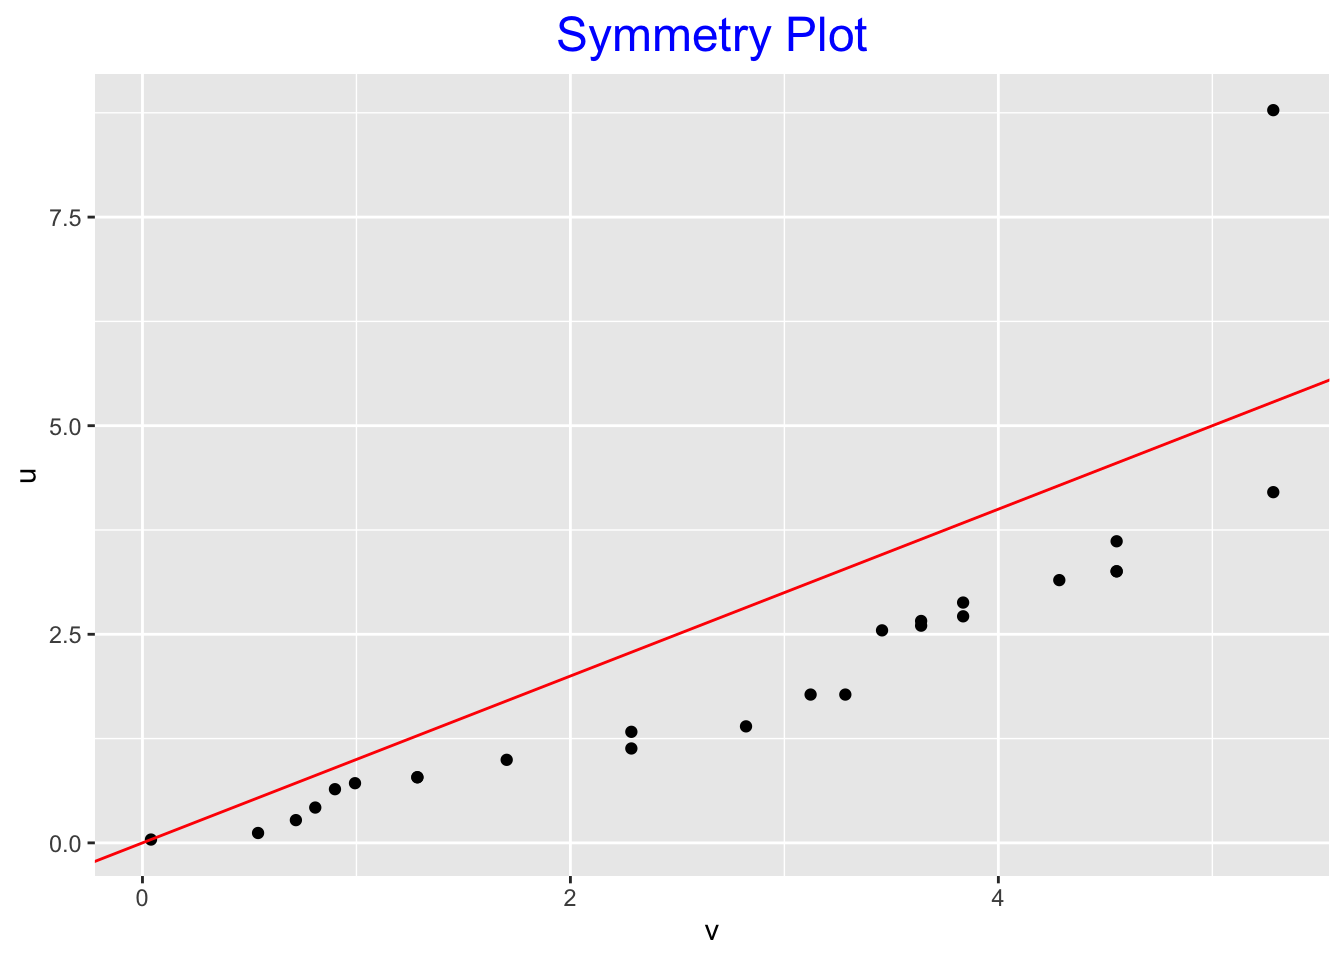
\includegraphics{Course-in-Exploratory-Data-Analysis_files/figure-latex/unnamed-chunk-59-1.pdf}

What do we see in the displays?

\begin{itemize}
\tightlist
\item
  \textbf{Stemplot} Here the roots look pretty uniform distributed from 0 to 100. Looking more carefully, I see some left-skewness in this 0-100 region. Also there is one outlier at the high end.
\item
  \textbf{Letter-value display} Actually, there is only a small trend, if any, in the sequence of midsummaries. There is a drop from the median to the mid-fourth, indicating some left skewness in the middle half of the data. Also, there is an increase from mid-C to mid-extreme, showing some right-skewness in the tails of the batch of roots.
\item
  \textbf{Symmetry plot} Practically all the points fall under the line u = v indicating left-skewness in the middle portion of the data. The only point above the line is at the far right, which is a reflection of the single outlier.
\end{itemize}

Let's continue down the ladder of powers and try the \(p = 0\) power (logs). Again, we show the stemplot, the letter-value display and the symmetry plot.

\begin{Shaded}
\begin{Highlighting}[]
\NormalTok{logs }\OtherTok{\textless{}{-}} \FunctionTok{log}\NormalTok{(farms}\SpecialCharTok{$}\NormalTok{count)}
\NormalTok{aplpack}\SpecialCharTok{::}\FunctionTok{stem.leaf}\NormalTok{(logs)}
\end{Highlighting}
\end{Shaded}

\begin{verbatim}
## 1 | 2: represents 1.2
##  leaf unit: 0.1
##             n: 50
##     2    0* | 00
##          0. | 
##     6    1* | 0003
##    10    1. | 7799
##    14    2* | 0134
##    16    2. | 77
##    24    3* | 02233444
##   (10)   3. | 6677888999
##    16    4* | 00011333344
##     5    4. | 5557
##     1    5* | 4
\end{verbatim}

\begin{Shaded}
\begin{Highlighting}[]
\FunctionTok{symplot}\NormalTok{(logs)}
\end{Highlighting}
\end{Shaded}

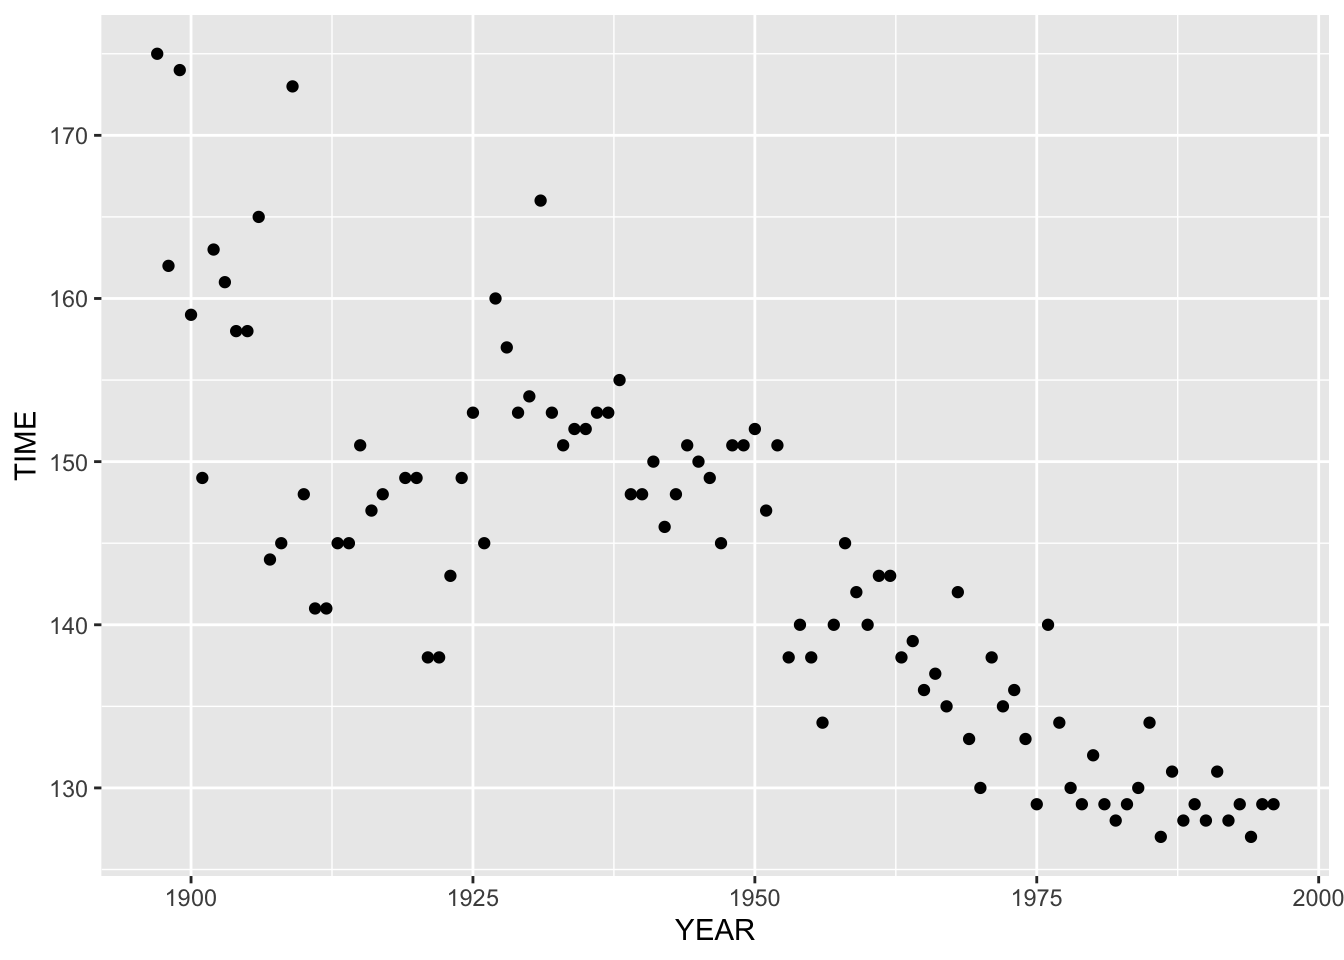
\includegraphics{Course-in-Exploratory-Data-Analysis_files/figure-latex/unnamed-chunk-60-1.pdf}

Here it should be clear that the logs of the farm numbers are left-skewed. The shape of the stemplot is left-skewed. The midsummaries are steadily decreasing and all the points in the symmetry plot are under the line, again reflecting the left-skewness.

\hypertarget{hinkleys-method}{%
\section{Hinkley's method}\label{hinkleys-method}}

A simple method of finding a suitable transformation, discussed in the last lecture, is based on Hinkley's \(d\) statistic, which is based on the difference between the mean and median.

Here are the values of the Hinkley statistic for the raw, root and log data.

\begin{Shaded}
\begin{Highlighting}[]
\FunctionTok{hinkley}\NormalTok{(farms}\SpecialCharTok{$}\NormalTok{count)}
\end{Highlighting}
\end{Shaded}

\begin{verbatim}
##          h 
## 0.08566038
\end{verbatim}

\begin{Shaded}
\begin{Highlighting}[]
\FunctionTok{hinkley}\NormalTok{(roots)}
\end{Highlighting}
\end{Shaded}

\begin{verbatim}
##          h 
## -0.0724257
\end{verbatim}

\begin{Shaded}
\begin{Highlighting}[]
\FunctionTok{hinkley}\NormalTok{(logs)}
\end{Highlighting}
\end{Shaded}

\begin{verbatim}
##          h 
## -0.2407449
\end{verbatim}

Since the raw data (\(p = 1\)) has a positive value of \(d\) and roots (\(p = .5\)) has a negative \(d\) value, this might suggest choosing a power reexpression (\(p\)) between .5 and 1. In this example, there is not a strong reason to reexpress, and roots might be a little more symmetric than the raw data.

\hypertarget{matched-transformations}{%
\section{Matched transformations}\label{matched-transformations}}

We are interested in comparing the effects of taking different reexpressions, such as taking logs and roots. But when we take a reexpression such as log, we mess up the scale of the raw data (logs are much smaller than the raw data), and so it is difficult to make a comparison.

It would be helpful if the raw and reexpressed data were roughly on the same scale so we can easily compare the two datasets. We can accomplish this by means of a procedure called matching.

In the following, we denote our raw data by \(x\)
and our reexpressed data by \(y = T(x)\).

Now we know that we can apply a further linear transformation which we can call
\[
z = a + b y = a + b T(x)
\]
The change from \(y\) to \(z\) is a trivial transformation and won't change the shape of the data.

We want to choose the constants \(a\) and \(b\) so that the \(z\) batch resembles the \(x\) batch. We can accomplish this in many ways. We describe two of them.

\hypertarget{matching-method-1}{%
\section{Matching Method 1}\label{matching-method-1}}

Here we choose two values in the raw scale (\(x\)) that will be the same in the new scale (\(z\)). Choose two points \(x_1\) and \(x_2\) in the original scale -- the corresponding points in the new scale will be \(z_1\) and \(z_2\). We wish to find values of the constants \(a\), \(b\) so that
\[
z_1= a + b T(x_1) = x_1
\]
\[
z_2 = a + b T(x_2) = x_2
\]

\hypertarget{matching-method-2}{%
\section{Matching Method 2}\label{matching-method-2}}

Here we choose one point that will be same in the raw (\(x\)) and new (\(z\)) scales. Also, by placing a condition on the derivative, we ensure that data close to the chosen value will be the same in the two scales. Choose point \(x_0\) such that
\[
z_0 = a + b T(x_0) = x_0
\]
and the derivative at z with respect to x at xo is equal to 1
\[
\frac{d}{dx}|_{x_0} = \frac{d[a+bT(x)]}{dx}|_{x_0}= b \frac{d T(x)}{dx}|_{x=x_0} = 1.
\]
If we solve for a and b from the two equations, we get the solution:
\[
z = x_0 + \frac{T(x) - T(x_0)}{T'(x_0)}.
\]
In usual practice, we choose \(x_0\) to be some central value in the raw data such as the median.

In the case of power functions, where the power \(p\) is not zero,
\[
T(x) = x^p,
\]
and the matching reexpression is
\[
z = x_0 + \frac{x^p - x_0^p}{p x_0^{p-1}}.
\]
In the case of the log (base 10) reexpression where \(T(x) = log(x)\), the matching transformation has the form
\[
z = x_0 + \frac{\log(x) -\log(x_0)}{\log(e)/x_0}.
\]

Let's illustrate matching for our farm numbers example. We use the second matching method and let \(x_0 = 39.5\), the median of the raw data. Using the above equations, we calculate the matching root and log transformations in R:

\begin{Shaded}
\begin{Highlighting}[]
\NormalTok{matched.roots }\OtherTok{\textless{}{-}} \FloatTok{39.5} \SpecialCharTok{+}\NormalTok{ (}\FunctionTok{sqrt}\NormalTok{(farms}\SpecialCharTok{$}\NormalTok{count) }\SpecialCharTok{{-}} 
                   \FunctionTok{sqrt}\NormalTok{(}\FloatTok{39.5}\NormalTok{)) }\SpecialCharTok{/}\NormalTok{ (.}\DecValTok{5}\SpecialCharTok{*}\FloatTok{39.5} \SpecialCharTok{\^{}}\NormalTok{ (}\SpecialCharTok{{-}}\NormalTok{.}\DecValTok{5}\NormalTok{))}
\NormalTok{matched.logs }\OtherTok{\textless{}{-}} \FloatTok{39.5} \SpecialCharTok{+}\NormalTok{ (}\FunctionTok{log10}\NormalTok{(farms}\SpecialCharTok{$}\NormalTok{count) }\SpecialCharTok{{-}} 
                   \FunctionTok{log10}\NormalTok{(}\FloatTok{39.5}\NormalTok{)) }\SpecialCharTok{/}\NormalTok{ (}\FunctionTok{log10}\NormalTok{(}\FunctionTok{exp}\NormalTok{(}\DecValTok{1}\NormalTok{)) }\SpecialCharTok{/} \FloatTok{39.5}\NormalTok{)}
\end{Highlighting}
\end{Shaded}

These calculations can also be done using the function \texttt{mtrans} in the \texttt{LearnBayes} package:

\begin{Shaded}
\begin{Highlighting}[]
\NormalTok{raw }\OtherTok{\textless{}{-}}\NormalTok{ farms}\SpecialCharTok{$}\NormalTok{count}
\NormalTok{matched.roots }\OtherTok{\textless{}{-}} \FunctionTok{mtrans}\NormalTok{(raw, }\FloatTok{0.5}\NormalTok{)}
\NormalTok{matched.logs }\OtherTok{\textless{}{-}} \FunctionTok{mtrans}\NormalTok{(raw, }\DecValTok{0}\NormalTok{)}
\end{Highlighting}
\end{Shaded}

To compare the raw, matched roots, and matched logs, we use parallel boxplots shown below.

\begin{Shaded}
\begin{Highlighting}[]
\FunctionTok{boxplot}\NormalTok{(}\FunctionTok{data.frame}\NormalTok{(raw, matched.roots, matched.logs))}
\end{Highlighting}
\end{Shaded}

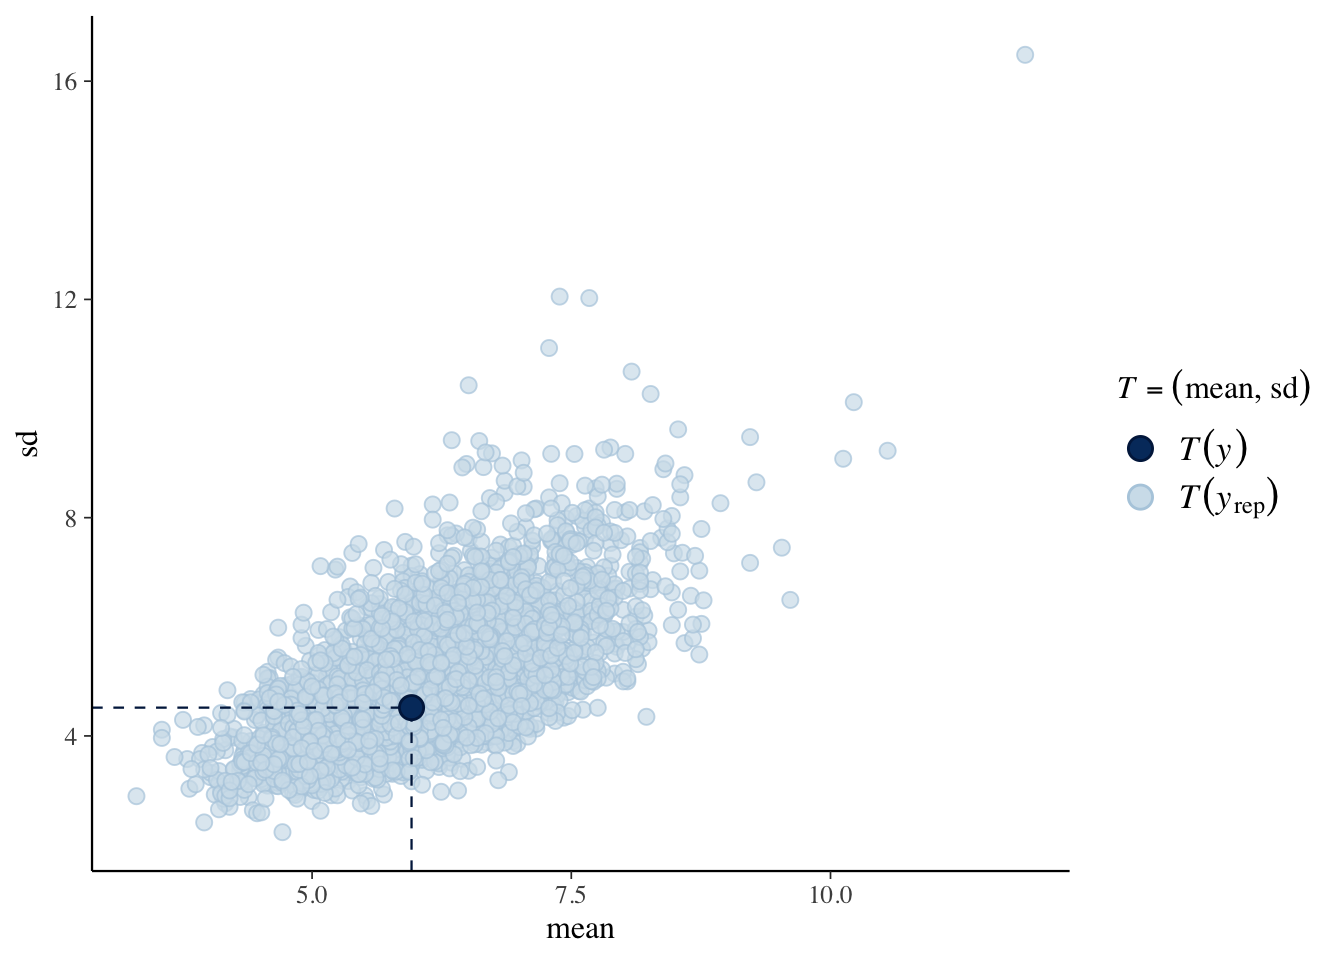
\includegraphics{Course-in-Exploratory-Data-Analysis_files/figure-latex/unnamed-chunk-64-1.pdf}

Note that this matching has given the three batches the same median (\(x_0\)) and the batches have similar spreads. We can focus on the shapes of the batches that is indicated by the position of the median within the box and the lengths of the whiskers.

What do we see in this boxplot display?

\begin{itemize}
\tightlist
\item
  Looking at the raw (farms) data, the middle 50\% of the data looks pretty symmetric and there is right skewness in the tails.
\item
  The roots are more symmetric in the tails, but this is offset by some left skewness in the middle 50\%.
\item
  The logs look left skewed both in the middle 50\% and the tails.
\end{itemize}

\hypertarget{transformations-summary}{%
\chapter{Transformations Summary}\label{transformations-summary}}

\hypertarget{why-do-we-reexpress-data}{%
\section{Why do we reexpress data?}\label{why-do-we-reexpress-data}}

We've focused here on two reasons to reexpress data:

\begin{itemize}
\tightlist
\item
  to make a batch symmetric
\item
  to stabilize spread across batches
\end{itemize}

Why are these desirable objectives?

A symmetric dataset is easier to view and summarize. Think of a normal curve (the best-known symmetric curve) -- once you know the mean and standard deviation, then you know about 2/3 of the data fall within one standard deviation of the mean.

Actually, the second objective is probably more important. We often wish to compare batches and this comparison is much easier when the spreads of the batches are approximately equal.

\hypertarget{serendipitous-effects-of-transformation}{%
\section{Serendipitous effects of transformation}\label{serendipitous-effects-of-transformation}}

After you work with data awhile, you'll discover that a reexpression that improves the batches with respect to one of these two objectives is likely to improve the batches with respect to the other objective. For example, if you are reexpressing to get equal spreads, you'll find that the reexpressed batches are more symmetric than the original batches.

Why? It has to do with the type of data we typically encountered.

When data are \textbf{COUNTS} or \textbf{AMOUNTS}, increasing spread with increasing level AND right skewness often occur together.

Think of a data set that contains some type of count. This data set is bounded below by 0. This will result in

\begin{itemize}
\tightlist
\item
  right skewness --small counts are constrained by 0 and large counts are not constrained -- this results in a pileup of data near 0
\item
  unequal spreads across batches. Due to the lower bound of 0, data sets that have small counts will have small spread. Data sets with larger counts don't have this bounding effect and will show more spread.
\end{itemize}

\hypertarget{when-is-it-worthwhile-to-transform}{%
\section{When is it worthwhile to transform?}\label{when-is-it-worthwhile-to-transform}}

There is one reason why one should not transform. It changes data to a less familiar scale and it will be harder to communicate the data to consumers.

But reexpression may be worthwhile when

\begin{itemize}
\tightlist
\item
  the range of the batch is large.
\end{itemize}

What is large? We want a large value of hi/lo. I don't want to set a precise definition of ``large'', but a ratio of hi/lo = 20 is good (reexpression may be helpful), and a ratio of hi/lo = 2 is not (reexpression won't help)

\begin{itemize}
\item
  there is a clear message from a transformation plot (such as the spread vs.~level plot)
\item
  there is some pattern in the residuals (we will discuss this later)
\end{itemize}

\hypertarget{introduction-to-plotting}{%
\chapter{Introduction to Plotting}\label{introduction-to-plotting}}

In this lecture, we introduce plotting of two-variable data and make some general comments about what we want to learn when we plot data.

\hypertarget{meet-the-data-2}{%
\section{Meet the data}\label{meet-the-data-2}}

Here is some data from one of the most famous track and field events, the Boston Marathon. This 26 mile race is run on Patriot's Day every April. It receives a lot of attention in the media and runners from all over the world compete. The table below (from the 2001 ESPN Information Please Sports Almanac) gives the winning time in minutes of the men's marathon for each year from 1950 to 2000. One interesting note is that the race has not always been the same length over the years. The length of the race was 26 miles, 385 through 1927-52 and all the years since 1957; it was (only) 25 miles, 958 yards in the years 1953-56.

This dataset is stored in \texttt{boston.marathon.wtimes} in the \texttt{LearnEDAfunctions} package.

\begin{Shaded}
\begin{Highlighting}[]
\FunctionTok{library}\NormalTok{(LearnEDAfunctions)}
\FunctionTok{library}\NormalTok{(tidyverse)}
\FunctionTok{head}\NormalTok{(boston.marathon.wtimes)}
\end{Highlighting}
\end{Shaded}

\begin{verbatim}
##   year minutes
## 1 1897     175
## 2 1898     162
## 3 1899     174
## 4 1900     159
## 5 1901     149
## 6 1902     163
\end{verbatim}

\hypertarget{graph-the-data}{%
\section{Graph the data}\label{graph-the-data}}

We are interested in how the race times change over the years. An obvious graph to make is a plot of TIME (vertical) against YEAR (horizontal) shown below. (This kind of graph is called a time-series plot, but we generally won't give graphs special names.)

\begin{Shaded}
\begin{Highlighting}[]
\FunctionTok{ggplot}\NormalTok{(boston.marathon.wtimes,}
       \FunctionTok{aes}\NormalTok{(year, minutes)) }\SpecialCharTok{+}
  \FunctionTok{geom\_point}\NormalTok{() }\SpecialCharTok{+}
  \FunctionTok{xlab}\NormalTok{(}\StringTok{"YEAR"}\NormalTok{) }\SpecialCharTok{+} \FunctionTok{ylab}\NormalTok{(}\StringTok{"TIME"}\NormalTok{)}
\end{Highlighting}
\end{Shaded}

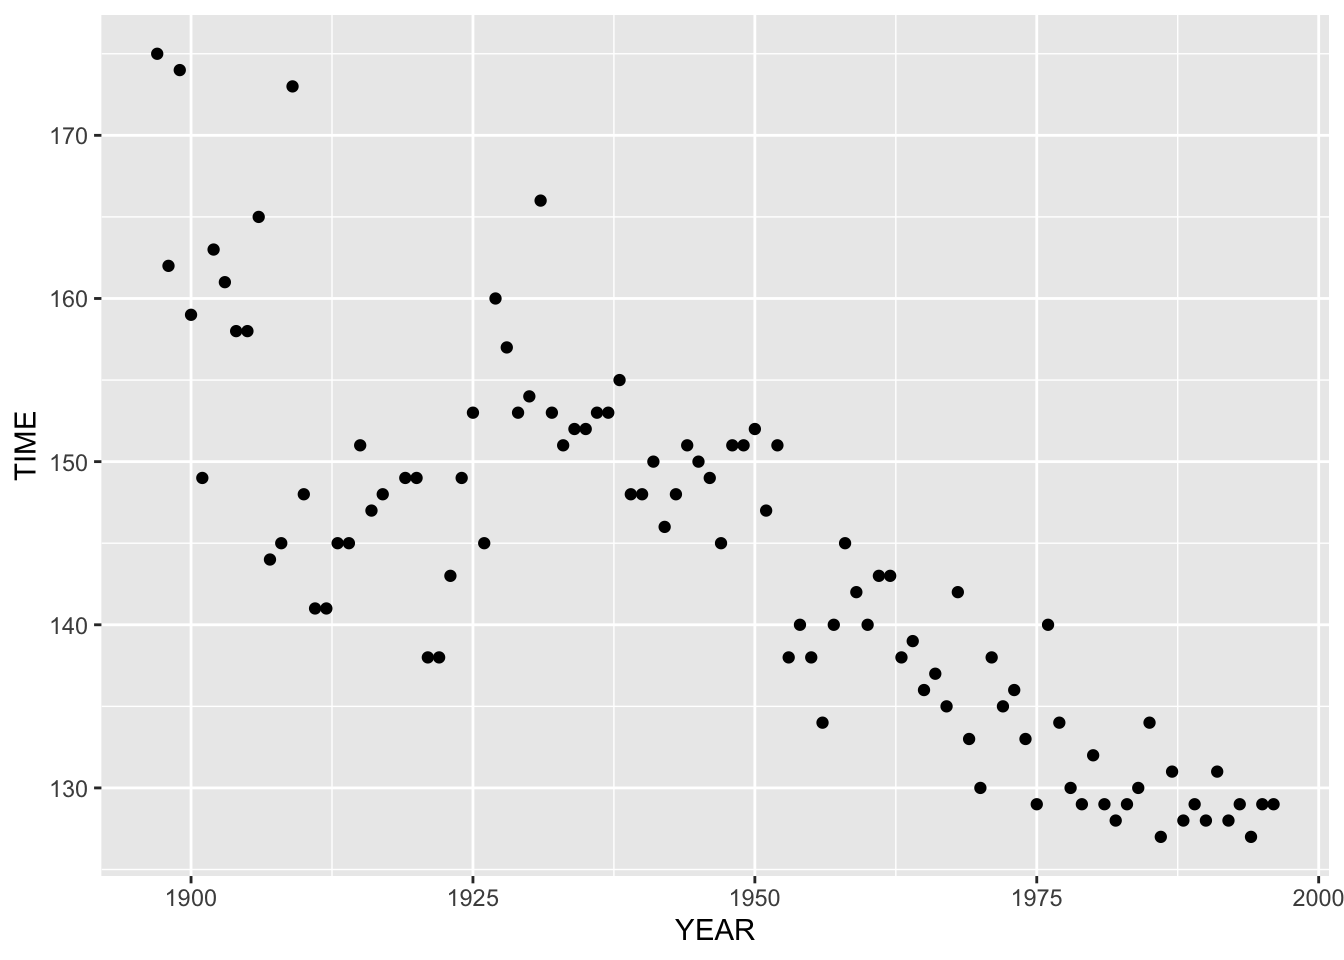
\includegraphics{Course-in-Exploratory-Data-Analysis_files/figure-latex/unnamed-chunk-66-1.pdf}

Looking at this graph, an obvious pattern is that the times are generally decreasing from 1950 to 2000. This means that the best runners are getting faster. We would notice this for practically all track-and-field events -- athletes are improving due to better equipment, better training, etc.

When we see a pattern, we want to describe it in some detailed way. It is sort of obvious that runners are getting faster, but what is the rate of this change?

\hypertarget{describing-the-fit}{%
\section{Describing the fit}\label{describing-the-fit}}

To find the rate at which the runners are getting faster, we want to fit a curve to the data. The simplest type of curve that we can fit is a line and we focus on fitting lines in this class. The pattern in the above scatterplot looks approximately linear (straight-line), so it seems reasonable to fit a line. The figure below shows the scatterplot with a line fit on top.

\begin{Shaded}
\begin{Highlighting}[]
\FunctionTok{ggplot}\NormalTok{(boston.marathon.wtimes,}
       \FunctionTok{aes}\NormalTok{(year, minutes)) }\SpecialCharTok{+}
  \FunctionTok{geom\_point}\NormalTok{() }\SpecialCharTok{+}
  \FunctionTok{geom\_smooth}\NormalTok{(}\AttributeTok{method =} \StringTok{"lm"}\NormalTok{, }\AttributeTok{se =} \ConstantTok{FALSE}\NormalTok{) }\SpecialCharTok{+}
  \FunctionTok{xlab}\NormalTok{(}\StringTok{"YEAR"}\NormalTok{) }\SpecialCharTok{+} \FunctionTok{ylab}\NormalTok{(}\StringTok{"TIME"}\NormalTok{)}
\end{Highlighting}
\end{Shaded}

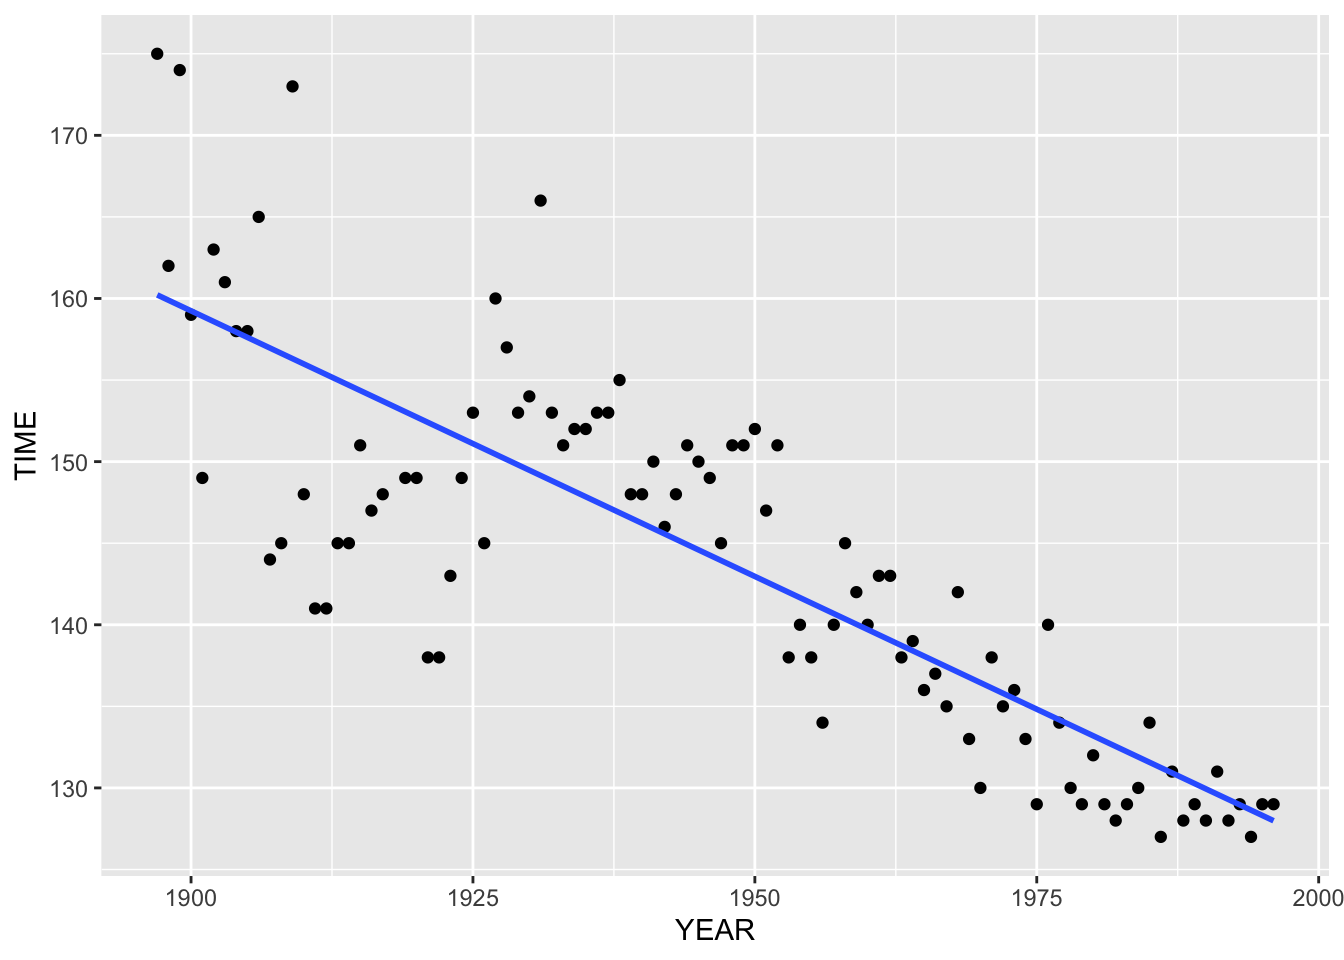
\includegraphics{Course-in-Exploratory-Data-Analysis_files/figure-latex/unnamed-chunk-67-1.pdf}

What is the interpretation of this line fit? The slope is \(m = -.3256\), so this means that the winning time in the marathon has generally been decreasing at a rate of .33 minutes (or about 20 seconds) per year. That's a pretty large rate of decrease. One wonders if the winning time will continue to decrease at this rate for future years.

\hypertarget{looking-at-the-residuals}{%
\section{Looking at the residuals}\label{looking-at-the-residuals}}

We've summarized the basic pattern in our scatterplot by using a line. But now we wish to look deeper. Is there any structure in these data beyond what we see in the general decrease in the winning time over years? To look for deeper structure, we look at the residuals. A residual is the difference between the observed winning time and its fit -- that is,
\[
RESIDUAL = ACTUAL TIME - FIT .
\]
Here the fit is the line
\[
FIT = -.3256 (YEAR - 1975) + 134.83
\]
We construct a residual plot by graphing the residuals (vertical) against the time (horizontal). We add a reference line at residual = 0 -- points close to this horizontal line are well-predicted using this fit.

\begin{Shaded}
\begin{Highlighting}[]
\NormalTok{boston.marathon.wtimes }\SpecialCharTok{\%\textgreater{}\%} 
  \FunctionTok{mutate}\NormalTok{(}\AttributeTok{FIT =} \SpecialCharTok{{-}}\NormalTok{.}\DecValTok{3256} \SpecialCharTok{*} 
\NormalTok{    (boston.marathon.wtimes}\SpecialCharTok{$}\NormalTok{year }\SpecialCharTok{{-}} \DecValTok{1975}\NormalTok{) }\SpecialCharTok{+} \FloatTok{134.83}\NormalTok{,}
    \AttributeTok{Residual =}\NormalTok{ minutes }\SpecialCharTok{{-}}\NormalTok{ FIT) }\SpecialCharTok{\%\textgreater{}\%} 
  \FunctionTok{ggplot}\NormalTok{(}\FunctionTok{aes}\NormalTok{(year, Residual)) }\SpecialCharTok{+} 
  \FunctionTok{geom\_point}\NormalTok{() }\SpecialCharTok{+}
  \FunctionTok{geom\_hline}\NormalTok{(}\AttributeTok{yintercept =} \DecValTok{0}\NormalTok{, }\AttributeTok{color =} \StringTok{"red"}\NormalTok{) }\SpecialCharTok{+}
  \FunctionTok{xlab}\NormalTok{(}\StringTok{"YEAR"}\NormalTok{)}
\end{Highlighting}
\end{Shaded}

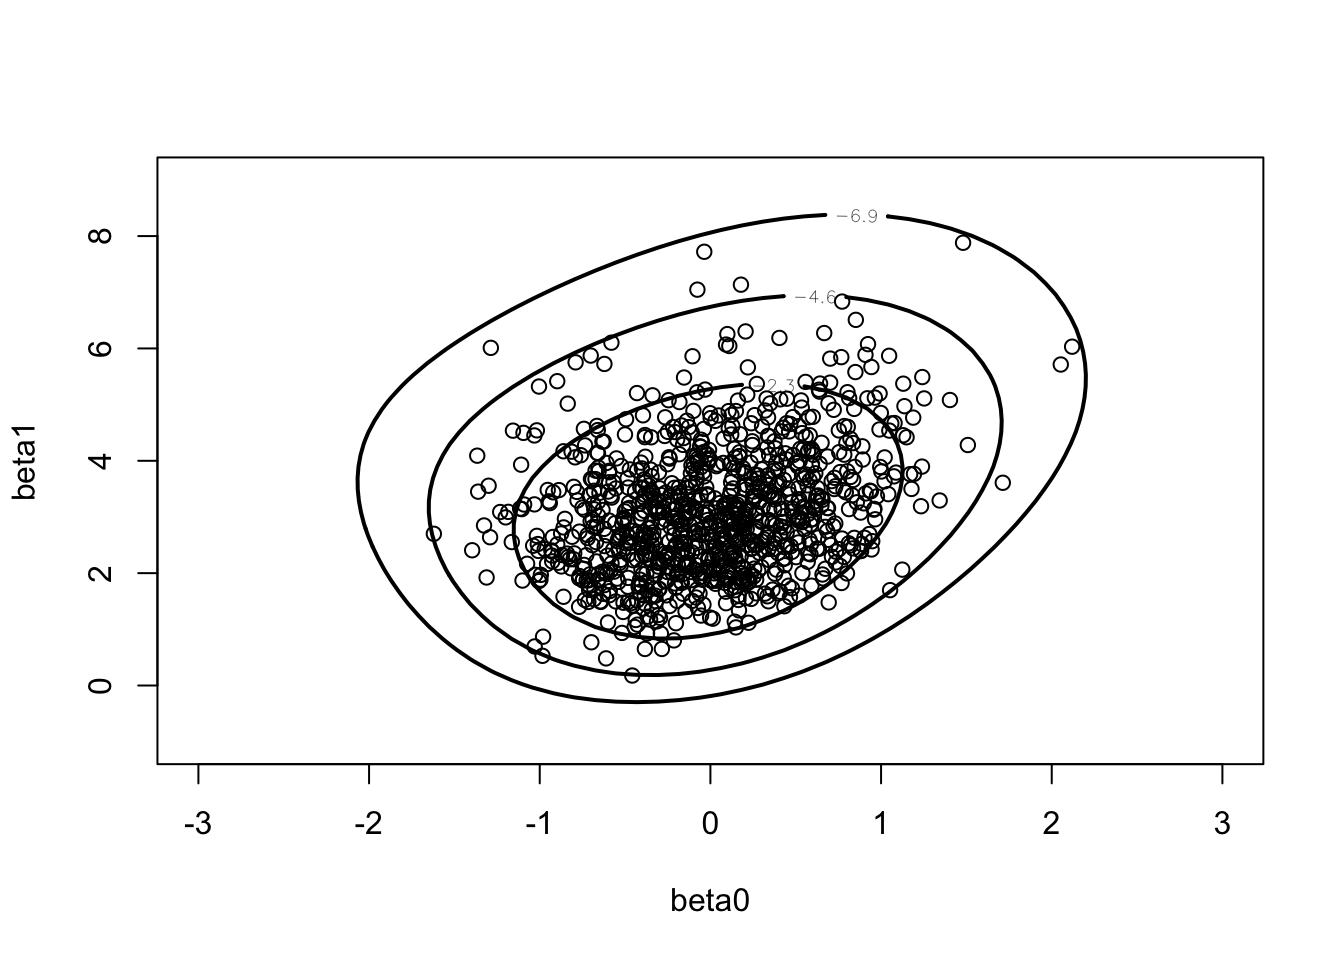
\includegraphics{Course-in-Exploratory-Data-Analysis_files/figure-latex/unnamed-chunk-68-1.pdf}

What do we see in this residual plot?

\begin{enumerate}
\def\labelenumi{\arabic{enumi}.}
\item
  First, note that there is no general trend, up or down, in this plot. We have removed the trend by subtracting the fit from the times. Since there is no trend, our eye won't be focusing at the general pattern that we saw earlier in our plot of time against year and we can look for deeper structure.
\item
  Although there is no general trend, I do notice a pattern in these residuals. The residuals for years 1950 until the early 1990's seem to be equally scattered on both sides of zero. However, the last six residuals are all positive. This means that the linear fit underestimates the winning time for these recent years.
\item
  Remember our earlier remark that the distance for the Boston Marathon was slightly smaller for the years 1953-1956? Looking at the residual plot, note that the residuals for these four years are all negative. This is what we would expect given the shorter length of the race for these years.
\item
  Another pattern that I notice in this plot is that there is a change in the variability of the residuals across time. The residuals from 1950 to 1980 generally fall between -5 and 5 minutes. But the residuals for the years 1980 through 2000 fall in a much tighter band about 0, suggesting that there is smaller variation in these winning times.
\item
  Another thing we look for in this plot is any unusually large residuals (positive or negative). There are a couple of extreme values, say 1950 and 1951 (positive) and 1956 (negative). But the 1950 and 1951 outliers are explained by the larger variation in best winning times for these early years, and we just explained that the negative residual in 1956 was explained by the shorter distance of the race.
\end{enumerate}

\hypertarget{an-alternative-fit}{%
\section{An alternative fit}\label{an-alternative-fit}}

The patterns in the residual plot suggest that maybe a line fit is not the best for these data. Later we will talk about a useful method called a resistant smooth of fitting a smooth curve through time series data.

We won't talk about the details of this smooth yet, but here is the result of this smooth applied to our marathon data.

\begin{Shaded}
\begin{Highlighting}[]
\FunctionTok{ggplot}\NormalTok{(boston.marathon.wtimes,}
       \FunctionTok{aes}\NormalTok{(year, minutes)) }\SpecialCharTok{+}
  \FunctionTok{geom\_point}\NormalTok{() }\SpecialCharTok{+}
  \FunctionTok{geom\_smooth}\NormalTok{(}\AttributeTok{method =} \StringTok{"loess"}\NormalTok{, }\AttributeTok{span =} \FloatTok{0.5}\NormalTok{, }
              \AttributeTok{se =} \ConstantTok{FALSE}\NormalTok{) }\SpecialCharTok{+}
  \FunctionTok{xlab}\NormalTok{(}\StringTok{"YEAR"}\NormalTok{) }\SpecialCharTok{+} \FunctionTok{ylab}\NormalTok{(}\StringTok{"TIME"}\NormalTok{)          }
\end{Highlighting}
\end{Shaded}

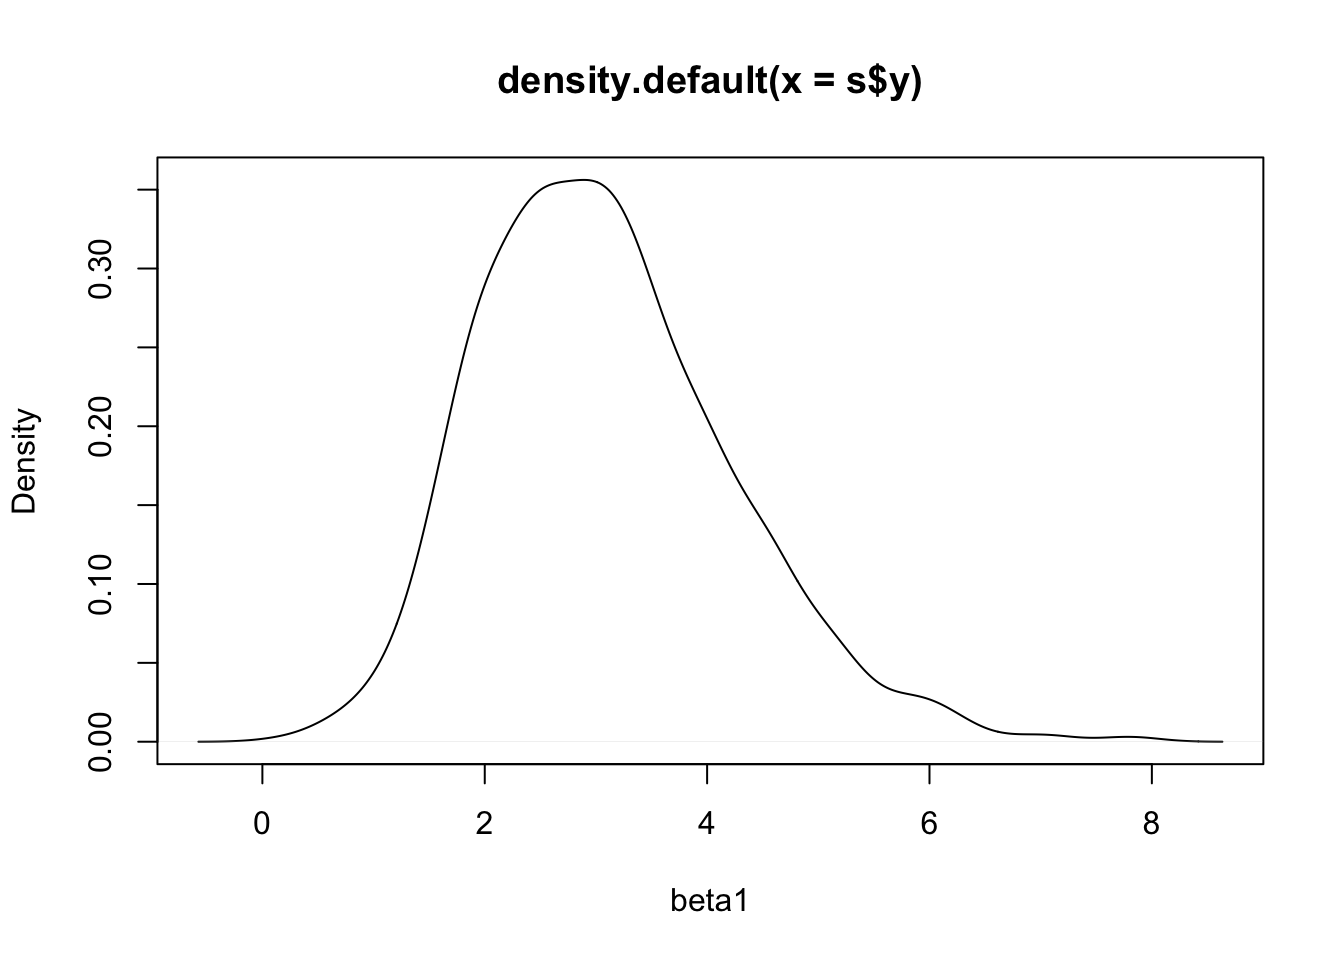
\includegraphics{Course-in-Exploratory-Data-Analysis_files/figure-latex/unnamed-chunk-69-1.pdf}

This smooth effectively shows some of the patterns in the graph that we observed earlier. There is a general decrease in the best winning time in the race over years. But \ldots{}

\begin{itemize}
\tightlist
\item
  there is a dip in the graph in the mid-50's -- we explained earlier this was due to the shorter running distance
\item
  there is a pretty steady decrease in the times between 1960 and 1980, although one might say that there is a leveling-off about 1970
\item
  the times since 1980 have stayed pretty constant, suggesting that maybe there is a leveling off in performance in this race
\end{itemize}

\hypertarget{resistant-line}{%
\chapter{Resistant Line}\label{resistant-line}}

In this lecture, we start to explore paired data where you suspect a relationship between \(x\) and \(y\). The focus here on how to fit a line to data in a ``resistant'' fashion, so the fit is relatively insensitive to extreme points.

\hypertarget{meet-the-data-3}{%
\section{Meet the data}\label{meet-the-data-3}}

Our data today is taken from the 2001 New York Times Almanac, p.~287. A table is shown which gives the median sales prices (in thousands of dollars) of existing single-family homes for selected metropolitan areas for the years 1985, 1990, 1995, 1999, and 2000. We will look only at the years 1985 and 2000 and delete the cities for which either the 1985 or the 2000 median house price is missing.

This dataset is available as \texttt{home.prices} in the \texttt{LearnEDAfunctions} package:

\begin{Shaded}
\begin{Highlighting}[]
\FunctionTok{library}\NormalTok{(LearnEDAfunctions)}
\FunctionTok{library}\NormalTok{(tidyverse)}
\FunctionTok{head}\NormalTok{(home.prices)}
\end{Highlighting}
\end{Shaded}

\begin{verbatim}
##         City y1985 y2000
## 1    Atlanta  66.2 125.4
## 2  Baltimore  72.6 145.2
## 3    Chicago  81.1 166.7
## 4 Cincinnati  60.2 124.0
## 5  Cleveland  64.4 121.3
## 6     Denver  84.3 181.5
\end{verbatim}

We start by plotting these data on a scatterplot where the \(x\) variable is the 1985 price and the \(y\) variable is the 2000 price. We get the following figure.

\begin{Shaded}
\begin{Highlighting}[]
\FunctionTok{ggplot}\NormalTok{(home.prices, }\FunctionTok{aes}\NormalTok{(y1985, y2000)) }\SpecialCharTok{+}
  \FunctionTok{geom\_point}\NormalTok{()}
\end{Highlighting}
\end{Shaded}

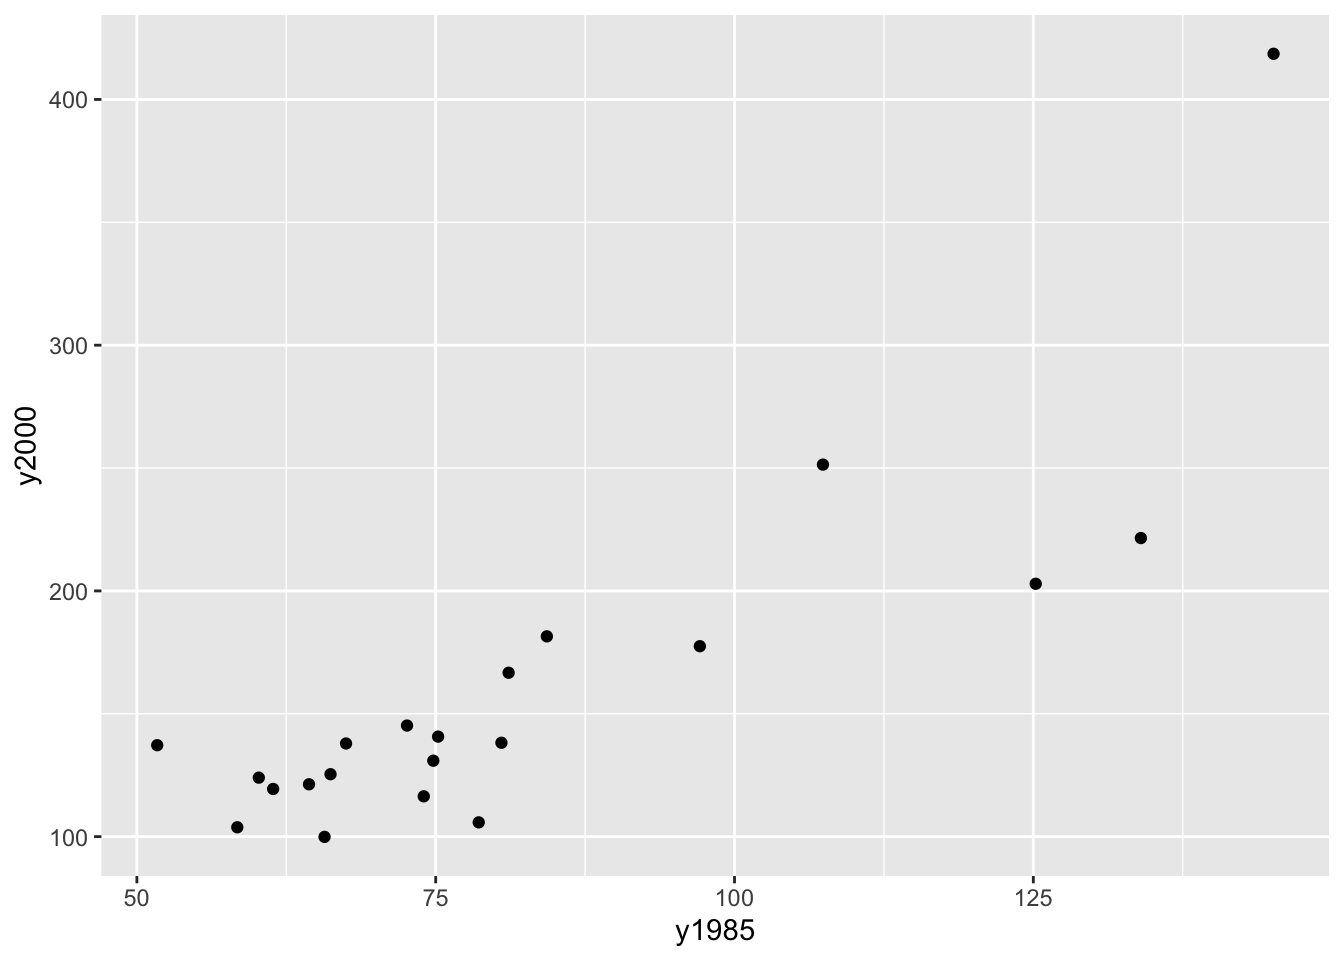
\includegraphics{Course-in-Exploratory-Data-Analysis_files/figure-latex/unnamed-chunk-71-1.pdf}

We see a positive trend in this graph which makes sense -- cities that had high house prices in 1985 tended also to have high prices in 2000. We want to describe this relationship using a simple function like a line.

But this is not the best graph of these data. Why? Well, most of the points fall in the lower left portion of the figure. This happens since both the set of 1985 house prices and the 2000 house prices are right skewed. We can improve this plot by reexpressing both the x and y variables by a power transformation. We'll talk more later about reexpressing variables in graphs, but take my word that a good reexpression to use in this case is a log.

If we take logs of both sets of house prices, we get a new scatterplot of the log (1985 prices) and log (2000 prices). Looking at the figure, note that the points are more evenly spread out -- from left to right and from down to up.

\begin{Shaded}
\begin{Highlighting}[]
\NormalTok{home.prices }\SpecialCharTok{\%\textgreater{}\%} 
  \FunctionTok{mutate}\NormalTok{(}\AttributeTok{log.1985 =} \FunctionTok{log10}\NormalTok{(y1985),}
         \AttributeTok{log.2000 =} \FunctionTok{log10}\NormalTok{(y2000)) }\OtherTok{{-}\textgreater{}}\NormalTok{ home.prices }
  \FunctionTok{ggplot}\NormalTok{(home.prices, }\FunctionTok{aes}\NormalTok{(log}\FloatTok{.1985}\NormalTok{, log}\FloatTok{.2000}\NormalTok{)) }\SpecialCharTok{+}
  \FunctionTok{geom\_point}\NormalTok{()}
\end{Highlighting}
\end{Shaded}

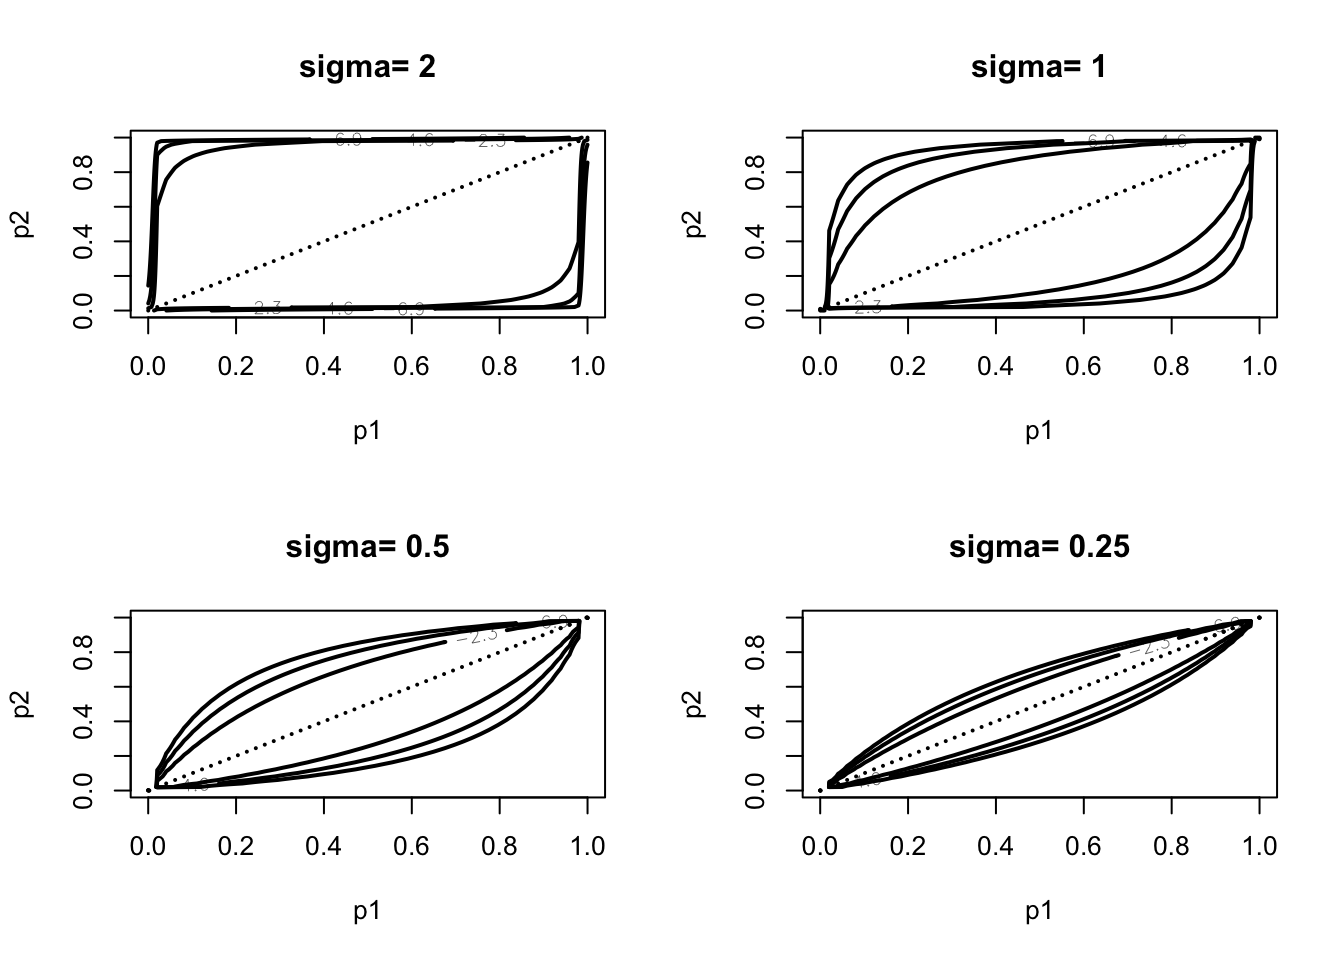
\includegraphics{Course-in-Exploratory-Data-Analysis_files/figure-latex/unnamed-chunk-72-1.pdf}

Since there appears to be a linear relationship between log (2000 price) and log (1985 price), it seems reasonable to fit a line. We describe a simple way of fitting a line that is not sensitive to outlying points -- we call this procedure a resistant line.

\hypertarget{three-summary-points}{%
\section{Three summary points}\label{three-summary-points}}

The first step to fitting a line

\begin{itemize}
\tightlist
\item
  divides the data into three groups and then
\item
  finds a summary point in each group
\end{itemize}

We divide the data by the \(x\)-values -- the lower third of the x-values form the first group, the middle third of the \(x\)-values form the 2nd group, and the upper third of the \(x\)-values make up the third group. This works fine if we have, say 15 points -- then an equal number will be in each group. If we have 16 points, it's reasonable to make the group sizes 5, 6, 5; if we have 17 points, then a symmetric way to go assigns 6, 5, 6 to the groups.

Here we have 21 cities, so there will be 7 cities in each group.

Our summary point for a group will be

\begin{verbatim}
(median x value, median y value).
\end{verbatim}

In the below table, the data has been sorted by 1985 price.

\begin{Shaded}
\begin{Highlighting}[]
\NormalTok{home.prices }\SpecialCharTok{\%\textgreater{}\%} 
  \FunctionTok{select}\NormalTok{(City, log}\FloatTok{.1985}\NormalTok{, log}\FloatTok{.2000}\NormalTok{) }\SpecialCharTok{\%\textgreater{}\%} 
  \FunctionTok{arrange}\NormalTok{(log}\FloatTok{.1985}\NormalTok{)}
\end{Highlighting}
\end{Shaded}

\begin{verbatim}
##             City log.1985 log.2000
## 1        Detroit 1.713491 2.137354
## 2          Tampa 1.766413 2.016197
## 3     Cincinnati 1.779596 2.093422
## 4    Kansas_City 1.788168 2.077004
## 5      Cleveland 1.808886 2.083861
## 6      St._Louis 1.817565 1.999565
## 7        Atlanta 1.820858 2.098298
## 8      Milwaukee 1.829304 2.139564
## 9      Baltimore 1.860937 2.161967
## 10  Philadelphia 1.869232 2.065953
## 11       Phoenix 1.873902 2.116940
## 12   Minneapolis 1.876218 2.148294
## 13       Houston 1.895423 2.024486
## 14         Miami 1.905796 2.140508
## 15       Chicago 1.909021 2.221936
## 16        Denver 1.925828 2.258877
## 17    Wash._D.C. 1.987219 2.249198
## 18     San_Diego 2.031004 2.400365
## 19   Los_Angeles 2.097604 2.307282
## 20 New_York_City 2.127105 2.345374
## 21 San_Francisco 2.161667 2.621799
\end{verbatim}

The first group consists of the seven cities with the smallest 1985 house prices. The median of the log 1985 prices for this group is 1.79 and the median of the log 2000 prices is 2.08 -- so the left summary point is
\[
(x_L, y_L) = (1.79, 2.08).
\]

In a similar fashion, we find summary points for the center and right groups:
\[
(x_C, y_C) =  (1.87, 2.14), \, \,    (x_R, y_R) = (2.03, 2.31).
\]
(Note that a summary point may or may not be an actual data point.)

In the figure below, we've drawn vertical lines showing the division of the points into three groups, and the summary points are indicated by red dots.

\begin{Shaded}
\begin{Highlighting}[]
\FunctionTok{ggplot}\NormalTok{(home.prices, }\FunctionTok{aes}\NormalTok{(log}\FloatTok{.1985}\NormalTok{, log}\FloatTok{.2000}\NormalTok{)) }\SpecialCharTok{+}
  \FunctionTok{geom\_point}\NormalTok{() }\SpecialCharTok{+}
  \FunctionTok{geom\_vline}\NormalTok{(}\AttributeTok{xintercept =} \FunctionTok{c}\NormalTok{(}\FloatTok{1.825}\NormalTok{, }\FloatTok{1.91}\NormalTok{)) }\SpecialCharTok{+}
  \FunctionTok{geom\_point}\NormalTok{(}\AttributeTok{data =} \FunctionTok{data.frame}\NormalTok{(}\AttributeTok{x=}\FunctionTok{c}\NormalTok{(}\FloatTok{1.79}\NormalTok{, }\FloatTok{1.87}\NormalTok{, }\FloatTok{2.03}\NormalTok{), }
                       \AttributeTok{y=}\FunctionTok{c}\NormalTok{(}\FloatTok{2.08}\NormalTok{, }\FloatTok{2.14}\NormalTok{, }\FloatTok{2.31}\NormalTok{)),}
             \FunctionTok{aes}\NormalTok{(x, y), }\AttributeTok{size =} \DecValTok{3}\NormalTok{, }\AttributeTok{color=}\StringTok{"red"}\NormalTok{,}
             \AttributeTok{shape =} \DecValTok{4}\NormalTok{, }\AttributeTok{stroke =} \DecValTok{2}\NormalTok{)}
\end{Highlighting}
\end{Shaded}

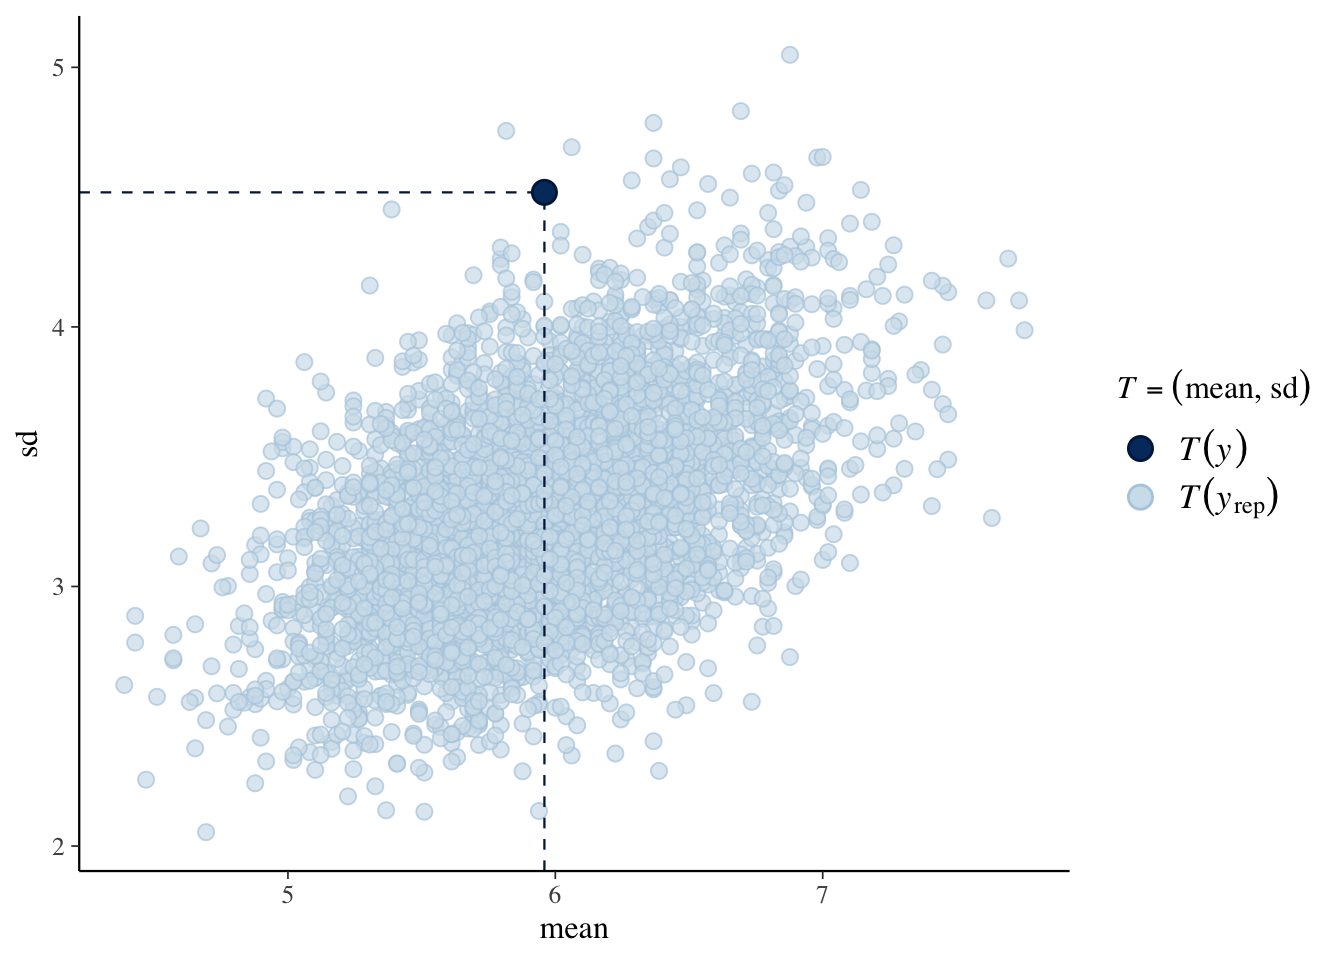
\includegraphics{Course-in-Exploratory-Data-Analysis_files/figure-latex/unnamed-chunk-74-1.pdf}

\hypertarget{fitting-a-line-to-three-points}{%
\section{Fitting a line to three points}\label{fitting-a-line-to-three-points}}

We all know how to fit a line that goes through two points. How about a line that goes through (approximately) three points?

We write the line in the form
\[
  y = a_0 + b_0 (x - x_C) ,
\]
where \(b_0\) is the slope and \(a_0\) is the value of \(y\) when \(x\) is equal to the middle summary point \(x_C\).

We find the slope of this line by using the left and right summary points:
\[
  b_0 = \frac{y_R - y_L}{x_R - x_L} .
\]
Actually, it is better to work with the summary points in R computed to higher precision. Here the slope would be

\begin{Shaded}
\begin{Highlighting}[]
\NormalTok{(b0 }\OtherTok{\textless{}{-}} \FloatTok{0.920}\NormalTok{)}
\end{Highlighting}
\end{Shaded}

\begin{verbatim}
## [1] 0.92
\end{verbatim}

To find the intercept, we first note that
\$
a\_0 = y - b\_0 (x - x\_C),
\$
and then define \(a_0\) to be the mean of the \{\(y - b_0(x - x_C)\)\}, averaged over the three summary points:
\[
a_0 = \frac{1}{3} \left([y_L - b_0 (x_L - x_C)] + y_C + [y_R - b_0 (x_R - x_C) ] \right).
\]
Here the intercept turns out to be

\begin{Shaded}
\begin{Highlighting}[]
\NormalTok{(a0 }\OtherTok{\textless{}{-}} \FloatTok{2.155}\NormalTok{)}
\end{Highlighting}
\end{Shaded}

\begin{verbatim}
## [1] 2.155
\end{verbatim}

So the three-group line is
\[          
          y = .920 (x - 1.87) + 2.155
\]\\
This line is graphed on the scatterplot below.

\begin{Shaded}
\begin{Highlighting}[]
\FunctionTok{ggplot}\NormalTok{(home.prices, }\FunctionTok{aes}\NormalTok{(log}\FloatTok{.1985}\NormalTok{, log}\FloatTok{.2000}\NormalTok{)) }\SpecialCharTok{+}
  \FunctionTok{geom\_point}\NormalTok{() }\SpecialCharTok{+}
  \FunctionTok{geom\_abline}\NormalTok{(}\AttributeTok{slope =} \FloatTok{0.920}\NormalTok{,}
              \AttributeTok{intercept =} \SpecialCharTok{{-}}\FloatTok{0.920} \SpecialCharTok{*} \FloatTok{1.87} \SpecialCharTok{+} \FloatTok{2.155}\NormalTok{) }
\end{Highlighting}
\end{Shaded}

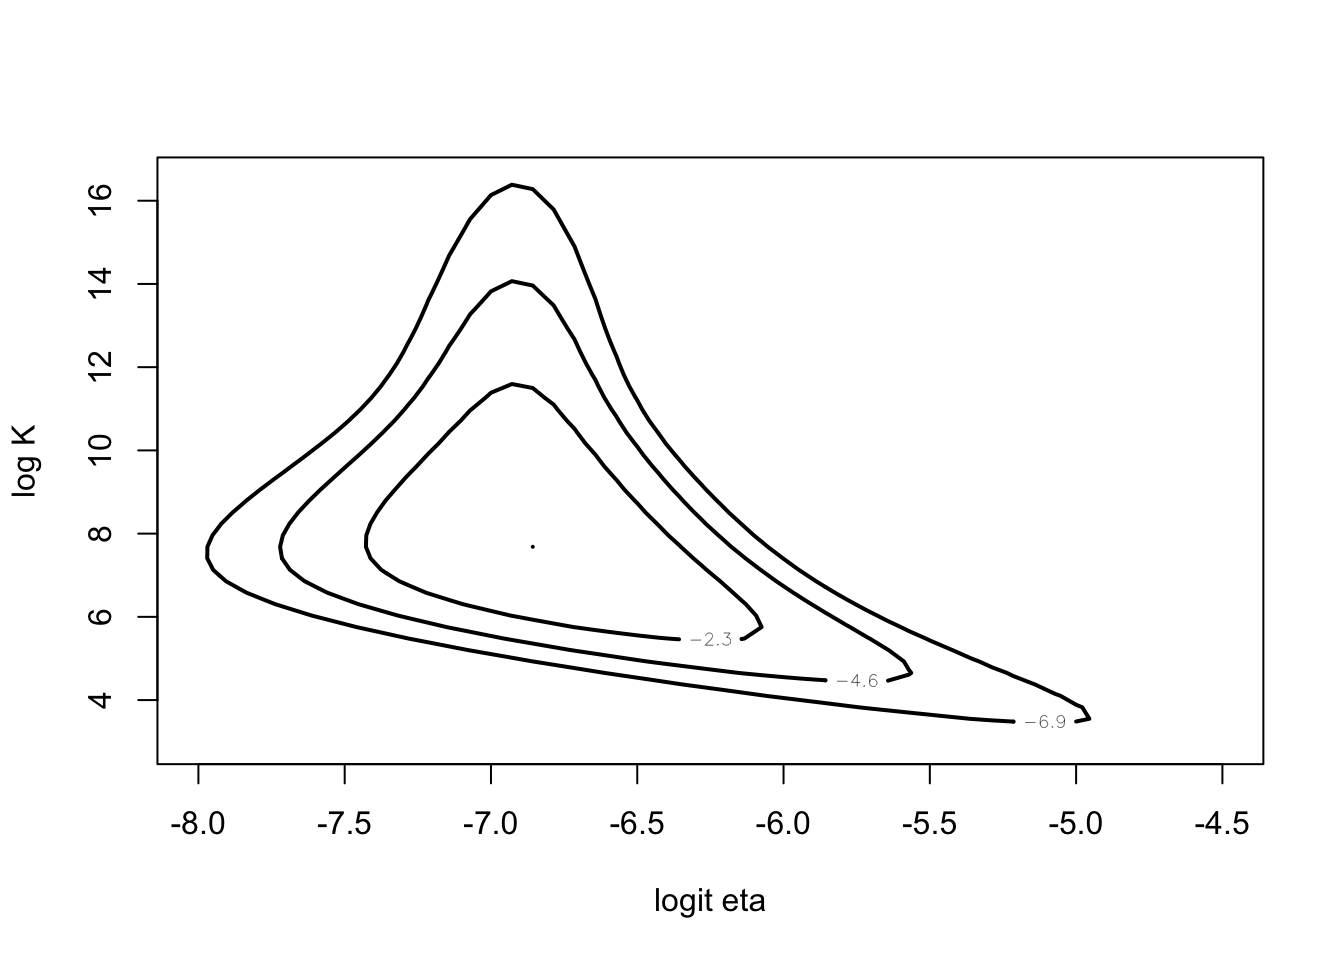
\includegraphics{Course-in-Exploratory-Data-Analysis_files/figure-latex/unnamed-chunk-77-1.pdf}

\hypertarget{improving-the-line-by-fitting-a-line-to-the-residuals}{%
\section{Improving the line by fitting a line to the residuals}\label{improving-the-line-by-fitting-a-line-to-the-residuals}}

Is this the best line through the points? To check, we examine the residuals which are the vertical deviations from the points to the line. A little more formally, we define a residual as
\[
          RESIDUAL = DATA - FIT,
\]
where \(DATA\) is the \(y\) value and \(FIT\) is the predicted value of \(y\) from the line fit:

\[           
            FIT = a_0 + b_0 (x - x_C).
\]

Let's find the residual for Detroit. Its \(y\) value (log 2000 house price) is \(DATA = 2.14\) and its predicted value from the line is
\[          
          FIT = .920 (1.71 - 1.87) + 2.155 = 2.01
\]\\
so Detroit's residual is
\[ 
          RESIDUAL = 2.14 - 2.01 = .013 .
\]

The following R code uses the function \texttt{rline} to fit a single iteration of the resistant line. Outputs of this function are the intercept and slope, value of \(x_C\), and the residuals. We create
a data frame that shows the fits and residuals for all cities.

\begin{Shaded}
\begin{Highlighting}[]
\NormalTok{myfit }\OtherTok{\textless{}{-}} \FunctionTok{rline}\NormalTok{(log}\FloatTok{.2000} \SpecialCharTok{\textasciitilde{}}\NormalTok{ log}\FloatTok{.1985}\NormalTok{, home.prices)}
\NormalTok{home.prices }\OtherTok{\textless{}{-}} 
  \FunctionTok{mutate}\NormalTok{(home.prices,}
         \AttributeTok{FIT =}\NormalTok{ myfit}\SpecialCharTok{$}\NormalTok{a }\SpecialCharTok{+}\NormalTok{ myfit}\SpecialCharTok{$}\NormalTok{b }\SpecialCharTok{*}\NormalTok{ (log}\FloatTok{.1985} \SpecialCharTok{{-}}\NormalTok{ myfit}\SpecialCharTok{$}\NormalTok{xC),}
         \AttributeTok{RESIDUAL =}\NormalTok{ log}\FloatTok{.2000} \SpecialCharTok{{-}}\NormalTok{ FIT)  }
\FunctionTok{select}\NormalTok{(home.prices, City, log}\FloatTok{.1985}\NormalTok{, log}\FloatTok{.2000}\NormalTok{, FIT, RESIDUAL)}
\end{Highlighting}
\end{Shaded}

\begin{verbatim}
##             City log.1985 log.2000      FIT      RESIDUAL
## 1        Atlanta 1.820858 2.098298 2.106212 -0.0079142188
## 2      Baltimore 1.860937 2.161967 2.143086  0.0188805053
## 3        Chicago 1.909021 2.221936 2.187326  0.0346095764
## 4     Cincinnati 1.779596 2.093422 2.068249  0.0251725826
## 5      Cleveland 1.808886 2.083861 2.095197 -0.0113360002
## 6         Denver 1.925828 2.258877 2.202789  0.0560875782
## 7        Detroit 1.713491 2.137354 2.007428  0.1299258047
## 8        Houston 1.895423 2.024486 2.174815 -0.1503292285
## 9    Kansas_City 1.788168 2.077004 2.076136  0.0008686638
## 10   Los_Angeles 2.097604 2.307282 2.360832 -0.0535502542
## 11         Miami 1.905796 2.140508 2.184359 -0.0438508423
## 12     Milwaukee 1.829304 2.139564 2.113982  0.0255819655
## 13   Minneapolis 1.876218 2.148294 2.157146 -0.0088515042
## 14 New_York_City 2.127105 2.345374 2.387974 -0.0426004858
## 15  Philadelphia 1.869232 2.065953 2.150718 -0.0847650389
## 16       Phoenix 1.873902 2.116940 2.155015 -0.0380748953
## 17     St._Louis 1.817565 1.999565 2.103182 -0.1036168913
## 18     San_Diego 2.031004 2.400365 2.299557  0.1008083642
## 19 San_Francisco 2.161667 2.621799 2.419774  0.2020256651
## 20         Tampa 1.766413 2.016197 2.056119 -0.0399221336
## 21    Wash._D.C. 1.987219 2.249198 2.259272 -0.0100741031
\end{verbatim}

We graph the residuals on the vertical axis against the log 1985 prices below.

\begin{Shaded}
\begin{Highlighting}[]
\FunctionTok{ggplot}\NormalTok{(home.prices, }\FunctionTok{aes}\NormalTok{(log}\FloatTok{.1985}\NormalTok{, RESIDUAL)) }\SpecialCharTok{+}
  \FunctionTok{geom\_point}\NormalTok{() }\SpecialCharTok{+}
  \FunctionTok{geom\_hline}\NormalTok{(}\AttributeTok{yintercept =} \DecValTok{0}\NormalTok{, }\AttributeTok{color =} \StringTok{"red"}\NormalTok{)}
\end{Highlighting}
\end{Shaded}

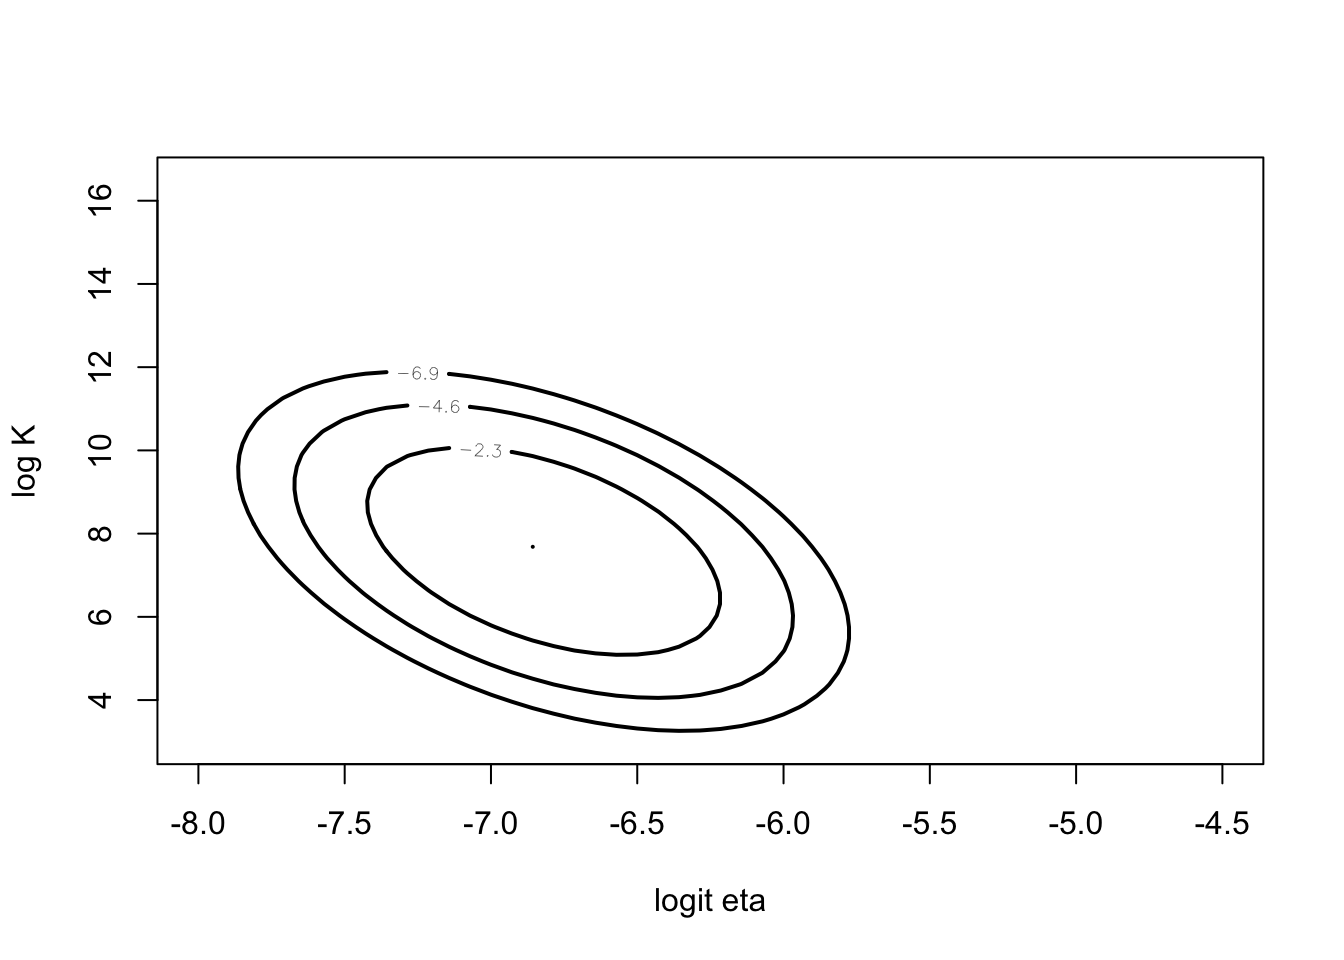
\includegraphics{Course-in-Exploratory-Data-Analysis_files/figure-latex/unnamed-chunk-79-1.pdf}

To see if we have fit a good line, we look for a pattern in the residuals. If there is some pattern -- say, the residual plot seems to be increasing, then this tells us that we can improve our line fit.

We try to improve our line fit by fitting a line to the \((x, RESIDUAL)\) data. We use the same 3-group method to fit our line. Some of the calculations are summarized in the table above.

\begin{itemize}
\item
  We first find three summary points. We already know the summary x values are 1.79, 1.87, 2.03. Looking at the residuals in each group, we find the summary residual values are respectively 0, -.03, .03. So our 3 summary points are
  \[         
          (1.79, 0), (1.87, -.03), (2.03, .03)
  \]
\item
  We find the slope d0 and the intercept g0 as we did before. The slope is
  \[ d0 = (.03 - 0) / (2.03 - 1.79) = .125\]
  and the intercept is
  \[
  g0 = 1/3[(0 - .125 (1.79 - 1.87)) + (-.03) + (.03 - .125 (2.03 - 1.87))] = -.003
  \]
  So our line fit to the (x, RESIDUAL) data is
  \[          
          RESID = -.003 + .125 (x - 1.87)
  \]
\item
  Our new fit to the \((x, y)\) data has the form
  \[          
          y = a_1 + b_1 (x - x_C),
   \]\\
  where we find the slope \(b_1\) and the intercept \(a_1\) are found by adding the slopes and intercepts from the two fits:
  \[
  b_1 = b_0 + d_0,  a_1 = a_0 + g_0.      
  \]
  Here
  \[ b_1 = .958 + .125 = 1.083, a_1 = 2.151 - .003 = 2.148.\]
  So our new fit to the data is
  \[          
          y = 1.083 (x - 1.87) + 2.15
  \]
\end{itemize}

Now we can continue this procedure as follows:

\begin{itemize}
\tightlist
\item
  Find the residuals from this fit.
\item
  Find three summary points of (x, RESID) and fit a 3-group line.
\item
  Update the slope and intercept of the fit to the (x, y) data.
\end{itemize}

In practice, we do this on R, and continue this procedure until there is little change in the adjustments to the slope and intercept.

For our example, I had the the function \texttt{rline} do ten iterations of this procedure with the following results (SLOPE is the current estimate of the slope of the resistant line and INTERCEPT is the current estimate at the intercept).

\begin{Shaded}
\begin{Highlighting}[]
\NormalTok{Results }\OtherTok{\textless{}{-}} \FunctionTok{data.frame}\NormalTok{(}\AttributeTok{Iteration=}\ConstantTok{NULL}\NormalTok{, }\AttributeTok{Slope=}\ConstantTok{NULL}\NormalTok{, }\AttributeTok{Intercept=}\ConstantTok{NULL}\NormalTok{)}
\ControlFlowTok{for}\NormalTok{(iterations }\ControlFlowTok{in} \DecValTok{1}\SpecialCharTok{:}\DecValTok{10}\NormalTok{)\{}
\NormalTok{  fit }\OtherTok{\textless{}{-}} \FunctionTok{rline}\NormalTok{(log}\FloatTok{.2000} \SpecialCharTok{\textasciitilde{}}\NormalTok{ log}\FloatTok{.1985}\NormalTok{, home.prices,  }
               \AttributeTok{iter=}\NormalTok{iterations)}
\NormalTok{  Results }\OtherTok{\textless{}{-}} \FunctionTok{rbind}\NormalTok{(Results,}
                   \FunctionTok{data.frame}\NormalTok{(}\AttributeTok{Iteration=}\NormalTok{iterations, }
                              \AttributeTok{Slope=}\NormalTok{fit}\SpecialCharTok{$}\NormalTok{b, }\AttributeTok{Intercept=}\NormalTok{fit}\SpecialCharTok{$}\NormalTok{a))}
\NormalTok{\}}
\NormalTok{Results}
\end{Highlighting}
\end{Shaded}

\begin{verbatim}
##    Iteration     Slope Intercept
## 1          1 0.9200503  2.155015
## 2          2 1.0951636  2.147055
## 3          3 1.2067010  2.149614
## 4          4 1.2777029  2.151248
## 5          5 1.3194267  2.152652
## 6          6 1.3439454  2.153477
## 7          7 1.3583537  2.153962
## 8          8 1.3668206  2.154247
## 9          9 1.3717961  2.154415
## 10        10 1.3747200  2.154513
\end{verbatim}

Note that after ten iterations, the procedure has essentially converged and the resistant line has equation
\[          
          y = 1.3747 (x - 1.87) + 2.1545
\]\\
This is typically the case, although there exist some examples where the procedure doesn't converge.

\hypertarget{comparison-with-a-least-squares-fit}{%
\section{Comparison with a Least-Squares Fit}\label{comparison-with-a-least-squares-fit}}

We have just described a resistant method of fitting a line. We should explain why this is preferable to the popular least-squares fit that you learned in your first stats course.

The least-squares fit to these data is given by

\begin{Shaded}
\begin{Highlighting}[]
\FunctionTok{lm}\NormalTok{(log}\FloatTok{.2000} \SpecialCharTok{\textasciitilde{}} \FunctionTok{I}\NormalTok{(log}\FloatTok{.1985} \SpecialCharTok{{-}} \FloatTok{1.87}\NormalTok{), }\AttributeTok{data=}\NormalTok{home.prices)}
\end{Highlighting}
\end{Shaded}

\begin{verbatim}
## 
## Call:
## lm(formula = log.2000 ~ I(log.1985 - 1.87), data = home.prices)
## 
## Coefficients:
##        (Intercept)  I(log.1985 - 1.87)  
##              2.148               1.044
\end{verbatim}

If you compare the resistant line with the least-squares line, they look pretty close. The slope of the resistant line is .88 which is a little bit smaller than the least-squares slope of 1.04.

The big difference between the two fits is how they react to outliers. To illustrate this, notice that San Francisco has an median house price of 418.6 (thousand dollars). Suppose instead that the median price was 1000, so log median price = 3.00 (instead of 2.62). What effect would this change have on our line fits?

We refit these data (with the unusally large price) using the resistant and least-squares methods.

\begin{Shaded}
\begin{Highlighting}[]
\NormalTok{home.prices }\SpecialCharTok{\%\textgreater{}\%} 
  \FunctionTok{mutate}\NormalTok{(}\AttributeTok{log.2000a =}\NormalTok{ log}\FloatTok{.2000}\NormalTok{,}
         \AttributeTok{log.2000a =} \FunctionTok{replace}\NormalTok{(log}\FloatTok{.2000}\NormalTok{a, y2000 }\SpecialCharTok{==} \FloatTok{418.6}\NormalTok{,}
                             \FloatTok{3.00}\NormalTok{)) }\OtherTok{{-}\textgreater{}}\NormalTok{ home.prices}

\FunctionTok{rline}\NormalTok{(log}\FloatTok{.2000}\NormalTok{a }\SpecialCharTok{\textasciitilde{}}\NormalTok{ log}\FloatTok{.1985}\NormalTok{, }
\NormalTok{      home.prices, }\DecValTok{5}\NormalTok{)[}\FunctionTok{c}\NormalTok{(}\StringTok{"a"}\NormalTok{, }\StringTok{"b"}\NormalTok{, }\StringTok{"xC"}\NormalTok{)]}
\end{Highlighting}
\end{Shaded}

\begin{verbatim}
## $a
## [1] 2.152652
## 
## $b
## [1] 1.319427
## 
## $xC
## [1] 1.873902
\end{verbatim}

\begin{Shaded}
\begin{Highlighting}[]
\FunctionTok{lm}\NormalTok{(log}\FloatTok{.2000}\NormalTok{a }\SpecialCharTok{\textasciitilde{}} \FunctionTok{I}\NormalTok{(log}\FloatTok{.1985} \SpecialCharTok{{-}} \FloatTok{1.874}\NormalTok{), }\AttributeTok{data =}\NormalTok{ home.prices)}
\end{Highlighting}
\end{Shaded}

\begin{verbatim}
## 
## Call:
## lm(formula = log.2000a ~ I(log.1985 - 1.874), data = home.prices)
## 
## Coefficients:
##         (Intercept)  I(log.1985 - 1.874)  
##               2.162                1.384
\end{verbatim}

The resistant line is
\[        
          y = 1.319 (x - 1.874) + 2.153
\]\\
which is identical to the line that we found earlier. The change in the largest house price had no effect on the fits since the resistant line is based on computing median values of \(x\) and \(y\) in each group.

In contrast, the least-squares fit with the large house price is
\[          
          y = - 0.408 + 1.38 x
\]\\
which is different from the earlier least-squares fit -- the slope has increased from 1.04 to 1.37. So a single extreme observation can have a big effect on the least-squares fit. The least-squares line suffers from the same lack-of-resistance problem as our familiar measure of center, the mean.

\hypertarget{interpreting-the-fit}{%
\section{Interpreting the fit}\label{interpreting-the-fit}}

Remember we initially reexpressed the house price data to logs -- can we express our ``best line'' in terms of the original house price data?

Our resistant line fit was
\[          
          y = 1.3747 (x - 1.87) + 2.1545
\]\\
or
\[
y = 1.3747 x -0.416189
\]\\
which means
\[        
          \log ({\rm house \, price \,  in \, 2000}) = 1.3747 \log(
          {\rm house \, price \, in \, 1985}) -0.416189.
\]

If we take each side to the 10th power, we get the equivalent equation
\[  
{\rm house \, price \, in \, 2000} = [{\rm house \, price \, in \, 2000}]^{1.3747} \times 10^{- 0.416}.
\]

So a linear fit to the \((\log x, \log y)\) data is the same as an exponential-type fit in the \((x, y)\) data.

\hypertarget{plotting-ii}{%
\chapter{Plotting II}\label{plotting-ii}}

As you know, the United States takes a census every 10 years. The dataset \texttt{us.pop} in the \texttt{LearnBayes} package displays the population of the U.S. during each census from 1790 to 2000.

\begin{Shaded}
\begin{Highlighting}[]
\FunctionTok{library}\NormalTok{(LearnEDAfunctions)}
\FunctionTok{library}\NormalTok{(tidyverse)}
\FunctionTok{head}\NormalTok{(us.pop)}
\end{Highlighting}
\end{Shaded}

\begin{verbatim}
##   YEAR  POP
## 1 1790  3.9
## 2 1800  5.3
## 3 1810  7.2
## 4 1820  9.6
## 5 1830 12.9
## 6 1840 17.1
\end{verbatim}

First we plot population against year. What do we see in this plot?

\begin{Shaded}
\begin{Highlighting}[]
\FunctionTok{ggplot}\NormalTok{(us.pop, }\FunctionTok{aes}\NormalTok{(YEAR, POP)) }\SpecialCharTok{+} 
  \FunctionTok{geom\_point}\NormalTok{() }\SpecialCharTok{+}
  \FunctionTok{ylab}\NormalTok{(}\StringTok{"Population"}\NormalTok{)}
\end{Highlighting}
\end{Shaded}

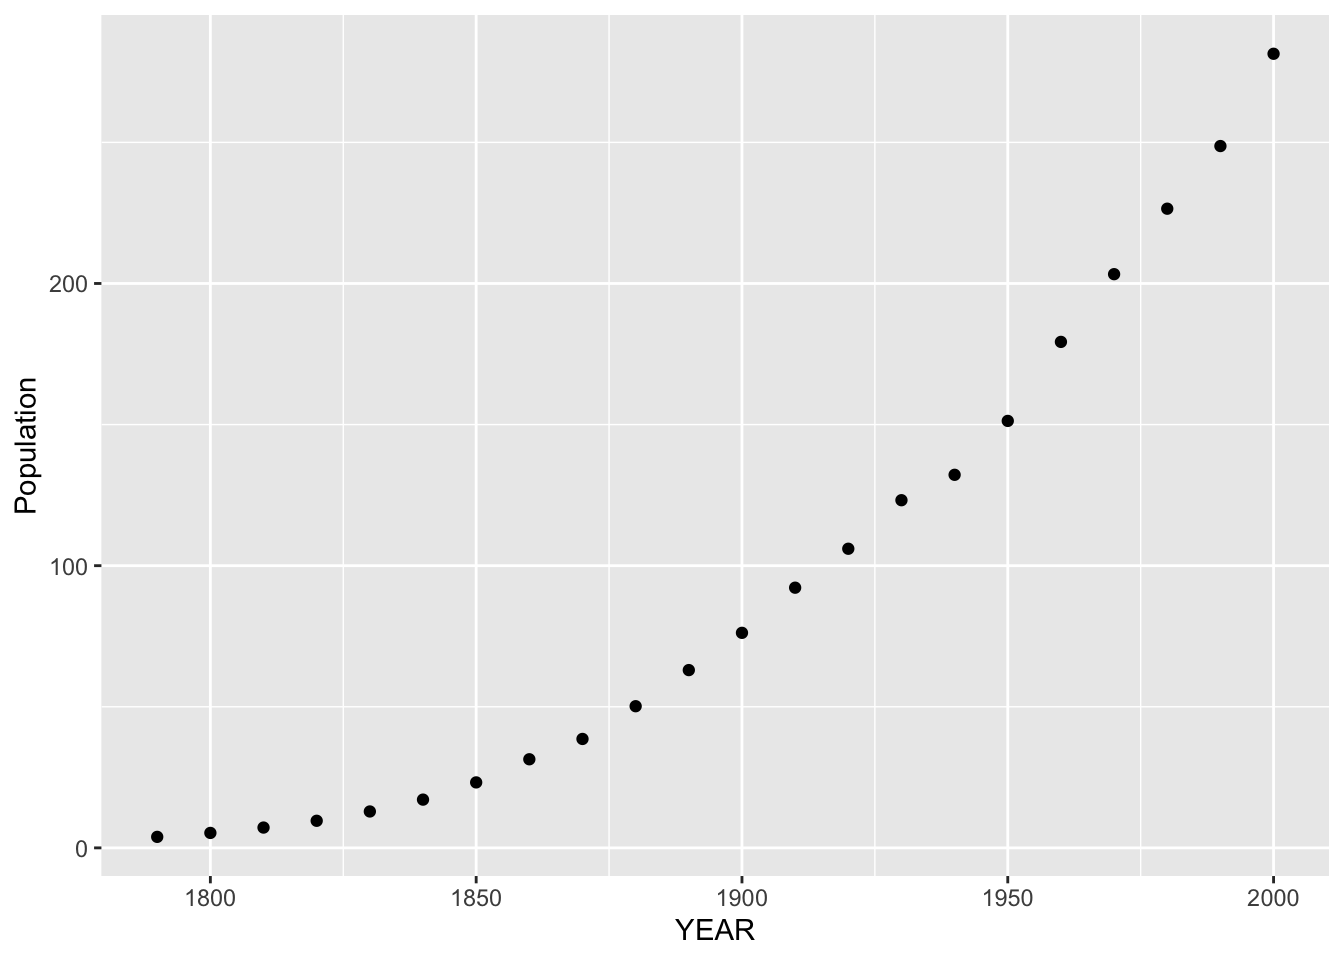
\includegraphics{Course-in-Exploratory-Data-Analysis_files/figure-latex/unnamed-chunk-84-1.pdf}

Obviously the population of the U.S. has been increasing over time and that's the main message from this graph. But we already knew about the increasing population. We want to learn more. Specifically \ldots{}

\begin{itemize}
\tightlist
\item
  Can we describe how the population has increased over time? In other words, what is the pattern of growth of the U.S. population?
  -Once we have a handle on the rate of population growth, are there years where the population was different from this general pattern of growth?
\end{itemize}

\hypertarget{fitting-a-line-to-the-population-in-the-later-years}{%
\section{Fitting a line to the population in the later years}\label{fitting-a-line-to-the-population-in-the-later-years}}

Now the simplest model that we can fit to these data is a line. Can we fit a line effectively to this graph? No -- one line won't fit these data well. There is strong curvature in the plot for the early years of the U.S. history.

However, the graph for the later years looks pretty linear and it makes some sense to fit a line to the right-half of the plot. On the figure below, I've drawn a line by eye to the last nine points.

\begin{Shaded}
\begin{Highlighting}[]
\FunctionTok{ggplot}\NormalTok{(us.pop, }\FunctionTok{aes}\NormalTok{(YEAR, POP)) }\SpecialCharTok{+} 
  \FunctionTok{geom\_point}\NormalTok{() }\SpecialCharTok{+}
  \FunctionTok{ylab}\NormalTok{(}\StringTok{"Population"}\NormalTok{) }\SpecialCharTok{+}
  \FunctionTok{geom\_abline}\NormalTok{(}\AttributeTok{slope =} \FloatTok{2.3404}\NormalTok{, }\AttributeTok{intercept =} \SpecialCharTok{{-}}\FloatTok{4403.7}\NormalTok{)}
\end{Highlighting}
\end{Shaded}

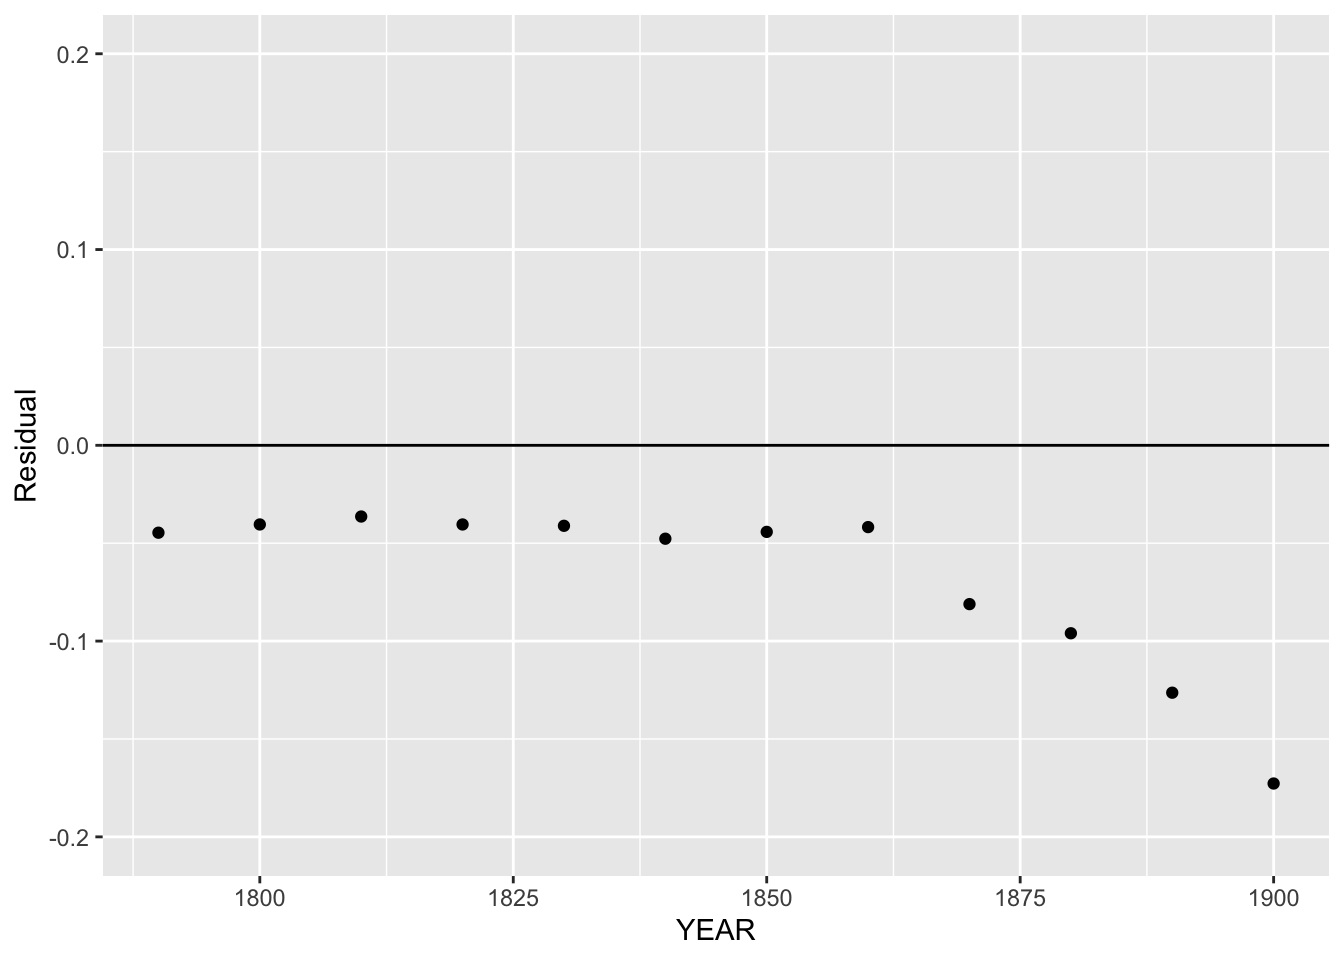
\includegraphics{Course-in-Exploratory-Data-Analysis_files/figure-latex/unnamed-chunk-85-1.pdf}

The equation of this line is
\[
FIT = 2.3404 \, YEAR - 4403.7
\]

The slope is 2.3 which means that, for the later years (1930 -- 2000), the population of the United States has been increasing by about 2.3 million each year.

After we have described the fit, then we look at the residuals. For each year, we compute

\[
RESIDUAL = POPULATION - FIT
\]
and we graph the residuals against the year.

\begin{Shaded}
\begin{Highlighting}[]
\NormalTok{us.pop }\SpecialCharTok{\%\textgreater{}\%} 
  \FunctionTok{mutate}\NormalTok{(}\AttributeTok{Fit =} \SpecialCharTok{{-}}\FloatTok{4403.7} \SpecialCharTok{+} \FloatTok{2.3404} \SpecialCharTok{*}\NormalTok{ YEAR,}
         \AttributeTok{Residual =}\NormalTok{ POP }\SpecialCharTok{{-}}\NormalTok{ Fit) }\OtherTok{{-}\textgreater{}}\NormalTok{ us.pop}
\FunctionTok{ggplot}\NormalTok{(us.pop, }\FunctionTok{aes}\NormalTok{(YEAR, Residual)) }\SpecialCharTok{+}
  \FunctionTok{geom\_point}\NormalTok{() }\SpecialCharTok{+}
  \FunctionTok{geom\_hline}\NormalTok{(}\AttributeTok{yintercept =} \DecValTok{0}\NormalTok{)}
\end{Highlighting}
\end{Shaded}

\includegraphics{Course-in-Exploratory-Data-Analysis_files/figure-latex/unnamed-chunk-86-1.pdf}

We notice the strong pattern in the residuals for the early years. This is expected, since the linear fit is only suitable for the population during the recent years. Actually, we don't care about the large residuals for the early years -- let's look at the residual graph only for the later years.

\begin{Shaded}
\begin{Highlighting}[]
\FunctionTok{ggplot}\NormalTok{(us.pop, }\FunctionTok{aes}\NormalTok{(YEAR, Residual)) }\SpecialCharTok{+}
  \FunctionTok{geom\_point}\NormalTok{() }\SpecialCharTok{+}
  \FunctionTok{geom\_hline}\NormalTok{(}\AttributeTok{yintercept =} \DecValTok{0}\NormalTok{) }\SpecialCharTok{+}
  \FunctionTok{xlim}\NormalTok{(}\DecValTok{1930}\NormalTok{, }\DecValTok{2000}\NormalTok{) }\SpecialCharTok{+} \FunctionTok{ylim}\NormalTok{(}\SpecialCharTok{{-}}\DecValTok{10}\NormalTok{, }\DecValTok{10}\NormalTok{)}
\end{Highlighting}
\end{Shaded}

\begin{verbatim}
## Warning: Removed 14 rows containing missing values (geom_point).
\end{verbatim}

\includegraphics{Course-in-Exploratory-Data-Analysis_files/figure-latex/unnamed-chunk-87-1.pdf}

The residuals in this graph look relatively constant, with a few notable exceptions:

\begin{itemize}
\tightlist
\item
  There is a large residual in 1930 which means that the population is higher than what is predicted using the linear model.
\item
  The residual in 1950 is smaller than the residuals in the surrounding years.
\item
  The residual in 2000 is somewhat large.
\end{itemize}

Can we provide any explanation for these small or large residuals? The major event in the 1940's was World War II. Many Americans participated in the war and I think this would account for some population decline -- maybe this explains the small residual in 1950. The large residuals in 1930 and 2000 mean that the rate of population growth in these years was a bit higher than the 2.3 million per year. To me the large residual in 2000 is the most interesting -- what is accounting for the extra population growth in the last ten years?

\hypertarget{fitting-a-line-to-the-log-population-in-the-early-years}{%
\section{Fitting a line to the log population in the early years}\label{fitting-a-line-to-the-log-population-in-the-early-years}}

Remember the curvature in the graph of population versus year that we saw in the early years? The interpretation of this curvature that the U.S. population growth in the early years was not linear but exponential. This means that the U.S. population was increasing at a constant rate during these formative years.

How can we summarize this exponential growth? First, we reexpress population by using a log -- the figure below plots the log population against year.

\begin{Shaded}
\begin{Highlighting}[]
\NormalTok{us.pop }\SpecialCharTok{\%\textgreater{}\%} \FunctionTok{mutate}\NormalTok{(}\AttributeTok{log.POP =} \FunctionTok{log10}\NormalTok{(POP)) }\OtherTok{{-}\textgreater{}}\NormalTok{ us.pop}
\FunctionTok{ggplot}\NormalTok{(us.pop, }\FunctionTok{aes}\NormalTok{(YEAR, log.POP)) }\SpecialCharTok{+}
  \FunctionTok{geom\_point}\NormalTok{()}
\end{Highlighting}
\end{Shaded}

\includegraphics{Course-in-Exploratory-Data-Analysis_files/figure-latex/unnamed-chunk-88-1.pdf}

Looking at this plot, it looks pretty much like a straight-line relationship for the early years. So we fit a line by eye:

\begin{Shaded}
\begin{Highlighting}[]
\FunctionTok{ggplot}\NormalTok{(us.pop, }\FunctionTok{aes}\NormalTok{(YEAR, log.POP)) }\SpecialCharTok{+}
  \FunctionTok{geom\_point}\NormalTok{() }\SpecialCharTok{+}
  \FunctionTok{geom\_abline}\NormalTok{(}\AttributeTok{slope =} \FloatTok{0.0129}\NormalTok{, }\AttributeTok{intercept =} \SpecialCharTok{{-}}\FloatTok{22.455}\NormalTok{)}
\end{Highlighting}
\end{Shaded}

\includegraphics{Course-in-Exploratory-Data-Analysis_files/figure-latex/unnamed-chunk-89-1.pdf}

This line has slope .0129 and intercept \(-22.455\), so our fit for log population for the early years is

\[
FIT (log population) = .0129 year - 22.455.
\]

If we take each side to the 10th power, then we get the relationship
\[
FIT (population) = 10^{.0129 year - 22.455}.
\]

Here \(10^{.0129} = 1.0301\), so the population of the U.S. was increasing by a 3 percent rate in the early years.

Looking further, we can compute residuals from our line fit to the (year, log population) data. Here the residual would be

\[
RESIDUAL = {\rm log \, population} - FIT ({\rm log \, population}).
\]

Here is the corresponding residual plot.

\begin{Shaded}
\begin{Highlighting}[]
\NormalTok{us.pop }\SpecialCharTok{\%\textgreater{}\%} 
  \FunctionTok{mutate}\NormalTok{(}\AttributeTok{LogFit =} \SpecialCharTok{{-}}\FloatTok{22.4553} \SpecialCharTok{+} \FloatTok{0.0129} \SpecialCharTok{*}\NormalTok{ YEAR,}
         \AttributeTok{Residual =}\NormalTok{ log.POP }\SpecialCharTok{{-}}\NormalTok{ LogFit) }\OtherTok{{-}\textgreater{}}\NormalTok{ us.pop}
\FunctionTok{ggplot}\NormalTok{(us.pop, }\FunctionTok{aes}\NormalTok{(YEAR, Residual)) }\SpecialCharTok{+}
  \FunctionTok{geom\_point}\NormalTok{() }\SpecialCharTok{+}
  \FunctionTok{geom\_hline}\NormalTok{(}\AttributeTok{yintercept =} \DecValTok{0}\NormalTok{)}
\end{Highlighting}
\end{Shaded}

\includegraphics{Course-in-Exploratory-Data-Analysis_files/figure-latex/unnamed-chunk-90-1.pdf}

We focus our attention to the early years where the fit was linear.

\begin{Shaded}
\begin{Highlighting}[]
\FunctionTok{ggplot}\NormalTok{(us.pop, }\FunctionTok{aes}\NormalTok{(YEAR, Residual)) }\SpecialCharTok{+}
  \FunctionTok{geom\_point}\NormalTok{() }\SpecialCharTok{+}
  \FunctionTok{geom\_hline}\NormalTok{(}\AttributeTok{yintercept =} \DecValTok{0}\NormalTok{) }\SpecialCharTok{+}
  \FunctionTok{xlim}\NormalTok{(}\DecValTok{1790}\NormalTok{, }\DecValTok{1900}\NormalTok{) }\SpecialCharTok{+}
  \FunctionTok{ylim}\NormalTok{(}\SpecialCharTok{{-}}\FloatTok{0.2}\NormalTok{, }\FloatTok{0.2}\NormalTok{)}
\end{Highlighting}
\end{Shaded}

\begin{verbatim}
## Warning: Removed 10 rows containing missing values (geom_point).
\end{verbatim}

\includegraphics{Course-in-Exploratory-Data-Analysis_files/figure-latex/unnamed-chunk-91-1.pdf}

I don't see any pattern in the residuals for the years 1790-1860, indicating that the line fit to the log population was pretty good in this time interval.

\hypertarget{straightening}{%
\chapter{Straightening}\label{straightening}}

We have talked about methods for working with \((x, y)\) data. First we graph the data to explore the relationship between \(x\) and \(y\), next we fit a simple line model to describe the relationship, and then we look at the residuals to look for finer structure in the data. In our U.S. population example, we saw that there may be a non-linear relationship in the plot, and we transformed the \(y\) variable (population) to first straighten the plot before we fit a line. In this lecture, we further discuss the situation where a non-linear pattern exists in the scatterplot, and discuss how we can reexpress the \(x\) and/or the \(y\) variables to make the pattern straight.

\hypertarget{meet-the-data-4}{%
\section{Meet the data}\label{meet-the-data-4}}

We work with a ``golden oldie'' dataset -- this is a dataset that has been used in the statistics literature to illustrate transforming data. This data is a nice illustration of a nonlinear relationship. The transformation of the \(x\) and \(y\) variables in this example suggests that the data may not have been measured in the most convenient scale.

A number of measurements were made on 38 1978-79 model automobiles. (Data was supplied by Consumer Reports and was used in the article ``Building Regression Models Interactively.'' by H. V. Henderson and P. F. Velleman (1981), Biometrics, 37, 391-411.)

For each car, we measure (1) the nationality of the manufacturer, (2) the name, (3) the mileage, measured in miles per gallon (MPG), (4) the weight, (5) the drive ratio, (6) the horsepower, (7) the displacement of the car (in cubic inches), and (8) the number of cylinders. The data follow:

\begin{Shaded}
\begin{Highlighting}[]
\FunctionTok{library}\NormalTok{(LearnEDAfunctions)}
\FunctionTok{library}\NormalTok{(tidyverse)}
\FunctionTok{head}\NormalTok{(car.measurements)}
\end{Highlighting}
\end{Shaded}

\begin{verbatim}
##   Country                       Car  MPG Weight Drive.Ratio Horsepower
## 1    U.S.        Buick_Estate_Wagon 16.9  4.360        2.73        155
## 2    U.S. Ford_Country_Squire_Wagon 15.5  4.054        2.26        142
## 3    U.S.        Chevy_Malibu_Wagon 19.2  3.605        2.56        125
## 4    U.S.    Chrysler_LeBaron_Wagon 18.5  3.940        2.45        150
## 5    U.S.                  Chevette 30.0  2.155        3.70         68
## 6   Japan             Toyota_Corona 27.5  2.560        3.05         95
##   Displacement Cylinders
## 1          350         8
## 2          351         8
## 3          267         8
## 4          360         8
## 5           98         4
## 6          134         4
\end{verbatim}

\hypertarget{a-nonlinear-relationship}{%
\section{A nonlinear relationship}\label{a-nonlinear-relationship}}

Here we explore the relationship between a car's mileage and it's displacement. Now most of us are aware of a relationship -- smaller cars generally get better gas mileage. Our goal here is to describe the relationship between size and mileage and look for cars that deviate from this general pattern.

We plot mileage against displacement below.

\begin{Shaded}
\begin{Highlighting}[]
\FunctionTok{ggplot}\NormalTok{(car.measurements,}
       \FunctionTok{aes}\NormalTok{(Displacement, MPG)) }\SpecialCharTok{+}
  \FunctionTok{geom\_point}\NormalTok{()}
\end{Highlighting}
\end{Shaded}

\includegraphics{Course-in-Exploratory-Data-Analysis_files/figure-latex/unnamed-chunk-93-1.pdf}

As expected, we see a pretty strong negative relationship. But what is evident is that this is not a straight-line relationship. Rather it looks curved -- a curve drawn through the points makes this clear.

\begin{Shaded}
\begin{Highlighting}[]
\FunctionTok{ggplot}\NormalTok{(car.measurements,}
       \FunctionTok{aes}\NormalTok{(Displacement, MPG)) }\SpecialCharTok{+}
  \FunctionTok{geom\_point}\NormalTok{() }\SpecialCharTok{+}
  \FunctionTok{geom\_smooth}\NormalTok{(}\AttributeTok{method =} \StringTok{"loess"}\NormalTok{, }\AttributeTok{se =} \ConstantTok{FALSE}\NormalTok{)}
\end{Highlighting}
\end{Shaded}

\includegraphics{Course-in-Exploratory-Data-Analysis_files/figure-latex/unnamed-chunk-94-1.pdf}

Recall what we did in our U.S. population study when we detected a curved relationship between population and year. We reexpressed the population using a log transformation and fit a line to the (year, log pop) data. We follow a similar strategy here. The difference is that we may reexpress the \(x\) and/or the \(y\) variables, and we use the family of power transformations (using different choices for the power \(p\)) in our reexpression.

\hypertarget{three-summary-points-and-measuring-curvature}{%
\section{Three summary points and measuring curvature}\label{three-summary-points-and-measuring-curvature}}

Recall that our method of fitting a line, the resistant line, is based on working with three summary points. Likewise, we use three summary points to measure the curvature in the plot and help us choose an appropriate reexpression to straighten.

As before, we find three summary points by breaking the \(x\)-values (here \(x\) is displacement) into three groups of approximate equal size (low, middle, and high), and finding the median \(x\)-value and the median \(y\)-value in each group. Here the three summary points are
\[
(x_L, y_L) = (98, 31), (x_M, y_M) = (148.5, 24.25), (x_R, y_R) = (302, 18.2).  
\]
These points are plotted as red dots in the figure below.

\begin{Shaded}
\begin{Highlighting}[]
\NormalTok{summary.points }\OtherTok{\textless{}{-}} \FunctionTok{data.frame}\NormalTok{(}\AttributeTok{x =} \FunctionTok{c}\NormalTok{(}\DecValTok{98}\NormalTok{, }\FloatTok{148.5}\NormalTok{, }\DecValTok{302}\NormalTok{),}
                             \AttributeTok{y =} \FunctionTok{c}\NormalTok{(}\DecValTok{31}\NormalTok{, }\FloatTok{24.25}\NormalTok{, }\FloatTok{18.2}\NormalTok{))}
\FunctionTok{ggplot}\NormalTok{(car.measurements,}
       \FunctionTok{aes}\NormalTok{(Displacement, MPG)) }\SpecialCharTok{+}
  \FunctionTok{geom\_point}\NormalTok{() }\SpecialCharTok{+}
  \FunctionTok{geom\_point}\NormalTok{(}\AttributeTok{data =}\NormalTok{ summary.points,}
              \FunctionTok{aes}\NormalTok{(x, y), }\AttributeTok{color=}\StringTok{"red"}\NormalTok{, }\AttributeTok{size =} \DecValTok{3}\NormalTok{)}
\end{Highlighting}
\end{Shaded}

\includegraphics{Course-in-Exploratory-Data-Analysis_files/figure-latex/unnamed-chunk-95-1.pdf}

We can measure the curvature in this plot by first computing the ``left slope'' (the slope of the line connecting the left and middle summary points), the ``right slope'' (the slope of the segment connecting the middle and right summary points). The ratio of the right slope to the left slope, the so-called half-slope ratio, is a measure of the curvature of the plot.

The figure below illustrates the computation of the half-slope ratio. The left slope of the segment connecting the left two points is
\[
m_L = (31-24.25)/(98-148.5) = -.144
\]
and the slope of the segment connecting the two right points is
\[
m_R = (24.25-18.2)/(148.5-302) = -.039.
\]

So the half-slope ratio, denoted \(b_{HS}\), is
\[
b_{HS} = \frac{m_R}{m_L} = \frac{-.039}{-.144} = .27.
\]

\begin{Shaded}
\begin{Highlighting}[]
\FunctionTok{ggplot}\NormalTok{() }\SpecialCharTok{+}
  \FunctionTok{geom\_point}\NormalTok{(}\AttributeTok{data =}\NormalTok{ car.measurements,}
       \FunctionTok{aes}\NormalTok{(Displacement, MPG)) }\SpecialCharTok{+}
  \FunctionTok{geom\_point}\NormalTok{(}\AttributeTok{data =}\NormalTok{ summary.points,}
              \FunctionTok{aes}\NormalTok{(x, y), }\AttributeTok{color=}\StringTok{"red"}\NormalTok{, }\AttributeTok{size =} \DecValTok{3}\NormalTok{) }\SpecialCharTok{+}
  \FunctionTok{geom\_smooth}\NormalTok{(}\AttributeTok{data =} \FunctionTok{filter}\NormalTok{(summary.points, x }\SpecialCharTok{\textless{}} \DecValTok{150}\NormalTok{),}
               \FunctionTok{aes}\NormalTok{(x, y), }\AttributeTok{method =} \StringTok{"lm"}\NormalTok{, }\AttributeTok{color=}\StringTok{"blue"}\NormalTok{) }\SpecialCharTok{+}
  \FunctionTok{geom\_smooth}\NormalTok{(}\AttributeTok{data =} \FunctionTok{filter}\NormalTok{(summary.points, x  }\SpecialCharTok{\textgreater{}} \DecValTok{145}\NormalTok{),}
               \FunctionTok{aes}\NormalTok{(x, y), }\AttributeTok{method =} \StringTok{"lm"}\NormalTok{, }\AttributeTok{color=}\StringTok{"blue"}\NormalTok{)}
\end{Highlighting}
\end{Shaded}

\begin{verbatim}
## Warning in qt((1 - level)/2, df): NaNs produced

## Warning in qt((1 - level)/2, df): NaNs produced
\end{verbatim}

\begin{verbatim}
## Warning in max(ids, na.rm = TRUE): no non-missing arguments to max; returning
## -Inf

## Warning in max(ids, na.rm = TRUE): no non-missing arguments to max; returning
## -Inf
\end{verbatim}

\includegraphics{Course-in-Exploratory-Data-Analysis_files/figure-latex/unnamed-chunk-96-1.pdf}

A half-slope ratio close to the value indicates straightness in the plot. Here the value \(b_{HS}\) = .27 which indicates curvature that is concave up.

\hypertarget{reexpressing-to-reduce-curvature}{%
\section{Reexpressing to reduce curvature}\label{reexpressing-to-reduce-curvature}}

In many cases, we can reduce the curvature in the plot by applying a suitable power transformation to either the \(x\) or \(y\) variables. Recall the ladder of power transformations:

We start with the raw data which corresponds to \(p = 1\) and either go up or down the ladder of transformations to change the shape of the data. How do we decide which direction on the ladder to transform the x and y variables? There is a simple rule based on the type of curvature in the plot.

Suppose that we observe a graph with the following curvature.

\includegraphics{Course-in-Exploratory-Data-Analysis_files/figure-latex/unnamed-chunk-97-1.pdf}

We look at the direction of the bulge in the curvature that we indicate by an arrow. Note that the curvature bulges towards small values of \(x\) and small values of \(y\). If the direction of the bulge for one variable goes towards small values, we go down the ladder of transformations; if the bulge is towards large values, we go up the ladder of transformations. Since this graph bulges towards small values for both variable, we can reexpress \(x\) by square root of \(x\), or log \(x\), or we could reexpress \(y\) by a root or a log.

Actually, there are four types of curvature that can be improved by a power transformation, shown below.

\includegraphics{Course-in-Exploratory-Data-Analysis_files/figure-latex/unnamed-chunk-98-1.pdf}

Once you see the direction of the bulge, the direction to transform the variables is clear. For example, look at the bottom right graph. The bulge in this curvature is towards small \(x\) and large \(y\). To straighten this plot, we could either

\begin{itemize}
\tightlist
\item
  reexpress \(x\) by a root (moving down the ladder) or
\item
  reexpress \(y\) by a square (moving up the ladder).
\end{itemize}

\hypertarget{straightening-in-the-example}{%
\section{Straightening in the example}\label{straightening-in-the-example}}

Let's illustrate this procedure for our data. We do our calculations in a spreadsheet where it is easy to change power transformations for \(x\) and \(y\). For ease of comparison of different transformations, we use the matched transformations
\[
\frac{x^p - 1}{p}, \, \, \frac{y^p - 1}{p}.
\]

Below we write a short function \texttt{straightening.work}
to illustrate the computations. We start with the original data -- the following table shows the left, center, and right summary points, the transformed summary points (tx, ty), the left and right slopes and the half-slope ratio. This is old news -- the ratio is .275 which indicates curvature in the plot.

\begin{Shaded}
\begin{Highlighting}[]
\NormalTok{straightening.work }\OtherTok{\textless{}{-}} \ControlFlowTok{function}\NormalTok{(sp, px, py)\{}
\NormalTok{   sp}\SpecialCharTok{$}\NormalTok{tx }\OtherTok{\textless{}{-}} \FunctionTok{with}\NormalTok{(sp, (x }\SpecialCharTok{\^{}}\NormalTok{ px }\SpecialCharTok{{-}} \DecValTok{1}\NormalTok{) }\SpecialCharTok{/}\NormalTok{ px)}
\NormalTok{   sp}\SpecialCharTok{$}\NormalTok{ty }\OtherTok{\textless{}{-}} \FunctionTok{with}\NormalTok{(sp, (y }\SpecialCharTok{\^{}}\NormalTok{ py }\SpecialCharTok{{-}} \DecValTok{1}\NormalTok{) }\SpecialCharTok{/}\NormalTok{ py)}
\NormalTok{   sp}\SpecialCharTok{$}\NormalTok{slope[}\DecValTok{1}\NormalTok{] }\OtherTok{\textless{}{-}} \FunctionTok{with}\NormalTok{(sp, }\FunctionTok{diff}\NormalTok{(ty[}\DecValTok{1}\SpecialCharTok{:}\DecValTok{2}\NormalTok{]) }\SpecialCharTok{/} \FunctionTok{diff}\NormalTok{(tx[}\DecValTok{1}\SpecialCharTok{:}\DecValTok{2}\NormalTok{]))}
\NormalTok{   sp}\SpecialCharTok{$}\NormalTok{slope[}\DecValTok{2}\NormalTok{] }\OtherTok{\textless{}{-}} \FunctionTok{with}\NormalTok{(sp, }\FunctionTok{diff}\NormalTok{(ty[}\DecValTok{2}\SpecialCharTok{:}\DecValTok{3}\NormalTok{]) }\SpecialCharTok{/} \FunctionTok{diff}\NormalTok{(tx[}\DecValTok{2}\SpecialCharTok{:}\DecValTok{3}\NormalTok{]))}
\NormalTok{   sp}\SpecialCharTok{$}\NormalTok{half.slope.ratio }\OtherTok{\textless{}{-}} \FunctionTok{with}\NormalTok{(sp, slope[}\DecValTok{2}\NormalTok{] }\SpecialCharTok{/}\NormalTok{ slope[}\DecValTok{1}\NormalTok{])}
\NormalTok{   sp}\SpecialCharTok{$}\NormalTok{slope[}\DecValTok{3}\NormalTok{] }\OtherTok{\textless{}{-}} \ConstantTok{NA}
\NormalTok{   sp}\SpecialCharTok{$}\NormalTok{half.slope.ratio[}\DecValTok{2}\SpecialCharTok{:}\DecValTok{3}\NormalTok{] }\OtherTok{\textless{}{-}} \ConstantTok{NA}
   \FunctionTok{row.names}\NormalTok{(sp) }\OtherTok{\textless{}{-}} \FunctionTok{c}\NormalTok{(}\StringTok{"Left"}\NormalTok{, }\StringTok{"Center"}\NormalTok{, }\StringTok{"Right"}\NormalTok{)}
\NormalTok{   sp\}}
\FunctionTok{straightening.work}\NormalTok{(summary.points, }\DecValTok{1}\NormalTok{, }\DecValTok{1}\NormalTok{)}
\end{Highlighting}
\end{Shaded}

\begin{verbatim}
##            x     y    tx    ty       slope half.slope.ratio
## Left    98.0 31.00  97.0 30.00 -0.13366337        0.2948727
## Center 148.5 24.25 147.5 23.25 -0.03941368               NA
## Right  302.0 18.20 301.0 17.20          NA               NA
\end{verbatim}

Remember the bulge is towards small values of \(x\) (displacement), so we'll try taking a square root of \(x\):

\begin{Shaded}
\begin{Highlighting}[]
\FunctionTok{straightening.work}\NormalTok{(summary.points, }\FloatTok{0.5}\NormalTok{, }\DecValTok{1}\NormalTok{)}
\end{Highlighting}
\end{Shaded}

\begin{verbatim}
##            x     y       tx    ty      slope half.slope.ratio
## Left    98.0 31.00 17.79899 30.00 -1.4760147        0.3947231
## Center 148.5 24.25 22.37212 23.25 -0.5826171               NA
## Right  302.0 18.20 32.75629 17.20         NA               NA
\end{verbatim}

This is better -- the half-slope ratio has increased from .275 to .368, but it's still not close to the goal value of 1. Let's go further down the ladder of transformations for \(x\) -- we'll try a log (\(p\) = 0) -- we actually use \(p\) = .001 in the spreadsheet that approximates a log.

\begin{Shaded}
\begin{Highlighting}[]
\FunctionTok{straightening.work}\NormalTok{(summary.points, }\FloatTok{0.001}\NormalTok{, }\DecValTok{1}\NormalTok{)}
\end{Highlighting}
\end{Shaded}

\begin{verbatim}
##            x     y       tx    ty      slope half.slope.ratio
## Left    98.0 31.00 4.595495 30.00 -16.163243        0.5244925
## Center 148.5 24.25 5.013109 23.25  -8.477499               NA
## Right  302.0 18.20 5.726763 17.20         NA               NA
\end{verbatim}

We're doing better -- the half-slope ratio is now .488. Let's now try to move towards straightness by reexpressing \(y\). The bulge goes towards small \(y\), so we'll try a log (\(p\) = 0) for \(y\) (mileage):

\begin{Shaded}
\begin{Highlighting}[]
\FunctionTok{straightening.work}\NormalTok{(summary.points, }\FloatTok{0.001}\NormalTok{, }\FloatTok{0.001}\NormalTok{)}
\end{Highlighting}
\end{Shaded}

\begin{verbatim}
##            x     y       tx       ty      slope half.slope.ratio
## Left    98.0 31.00 4.595495 3.439890 -0.5899825         0.683707
## Center 148.5 24.25 5.013109 3.193505 -0.4033752               NA
## Right  302.0 18.20 5.726763 2.905635         NA               NA
\end{verbatim}

The ratio is now \(b_{HS}\) = .642 (the power for \(x\) is \(p\) = 0, for \(y\) is \(p\) =0). Let's keep going down the ladder for \(y\) and try \(p\) = -1 that corresponds to reciprocals.

\begin{Shaded}
\begin{Highlighting}[]
\FunctionTok{straightening.work}\NormalTok{(summary.points, }\FloatTok{0.001}\NormalTok{, }\SpecialCharTok{{-}}\DecValTok{1}\NormalTok{)}
\end{Highlighting}
\end{Shaded}

\begin{verbatim}
##            x     y       tx        ty       slope half.slope.ratio
## Left    98.0 31.00 4.595495 0.9677419 -0.02150082        0.8933663
## Center 148.5 24.25 5.013109 0.9587629 -0.01920811               NA
## Right  302.0 18.20 5.726763 0.9450549          NA               NA
\end{verbatim}

Now we're close -- \(b_{HS} = .845\). Last, we try moving \(x\) down the ladder to \(p = -.33\) (we'll explain this choice soon).

\begin{Shaded}
\begin{Highlighting}[]
\FunctionTok{straightening.work}\NormalTok{(summary.points, }\SpecialCharTok{{-}}\FloatTok{0.33}\NormalTok{, }\SpecialCharTok{{-}}\DecValTok{1}\NormalTok{)}
\end{Highlighting}
\end{Shaded}

\begin{verbatim}
##            x     y       tx        ty      slope half.slope.ratio
## Left    98.0 31.00 2.362910 0.9677419 -0.1049744         1.074659
## Center 148.5 24.25 2.448446 0.9587629 -0.1128117               NA
## Right  302.0 18.20 2.569958 0.9450549         NA               NA
\end{verbatim}

Bingo -- the half-slope ratio is \(b_{HS}\) = 1.017, so it appears that we've straightened the plot by transforming \(x\) to the -1/3 power and \(y\) to the -1 power.

\hypertarget{making-sense-of-the-reexpression}{%
\section{Making sense of the reexpression}\label{making-sense-of-the-reexpression}}

We started by plotting mileage against displacement of a car, where mileage was measured in miles per gallon and displacement is measured in cubic inches. What are the units of the transformed variables? If we change mileage to mileage\(^{-1}\), then the units are gallons per mile; if we change displacement to displacement\(^{-1/3}\), the new units are 1/inches. So we have found a linear relationship between
mileage (in gallons per mile) and displacement (measured as 1/inches).

This suggests that gallons per mile may be a more suitable scale for measuring mileage.

\hypertarget{straightening-fitting-and-flattening}{%
\section{Straightening, fitting, and flattening}\label{straightening-fitting-and-flattening}}

We found a suitable transformation by working only on three summary points. We have to check out our proposed reexpression to see if we have indeed straightened the plot

In the plot below, we graph \(-1/y\) against \(-1/x^{.33}\).

\begin{Shaded}
\begin{Highlighting}[]
\NormalTok{car.measurements }\OtherTok{\textless{}{-}} \FunctionTok{mutate}\NormalTok{(car.measurements,}
                    \AttributeTok{new.x =}\NormalTok{ Displacement }\SpecialCharTok{\^{}}\NormalTok{ (}\SpecialCharTok{{-}} \FloatTok{0.33}\NormalTok{),}
                    \AttributeTok{new.y =} \SpecialCharTok{{-}} \DecValTok{1} \SpecialCharTok{/}\NormalTok{ MPG)}
\FunctionTok{ggplot}\NormalTok{(car.measurements, }\FunctionTok{aes}\NormalTok{(new.x, new.y)) }\SpecialCharTok{+}
  \FunctionTok{geom\_point}\NormalTok{()}
\end{Highlighting}
\end{Shaded}

\includegraphics{Course-in-Exploratory-Data-Analysis_files/figure-latex/unnamed-chunk-105-1.pdf}

This looks pretty straight. To detect any remaining curvature, we will fit a line and inspect the residuals.

\begin{Shaded}
\begin{Highlighting}[]
\NormalTok{fit }\OtherTok{\textless{}{-}} \FunctionTok{rline}\NormalTok{(new.y }\SpecialCharTok{\textasciitilde{}}\NormalTok{ new.x, }
\NormalTok{             car.measurements, }\AttributeTok{iter=}\DecValTok{5}\NormalTok{)}
\FunctionTok{c}\NormalTok{(fit}\SpecialCharTok{$}\NormalTok{a, fit}\SpecialCharTok{$}\NormalTok{b, fit}\SpecialCharTok{$}\NormalTok{xC)}
\end{Highlighting}
\end{Shaded}

\begin{verbatim}
## [1] -0.04249751  0.34584665  0.19202478
\end{verbatim}

We fit a line shown below -- it has intercept \(-0.0424\), slope \(-0.3458\), and \(x_C = -0.1920\), so our line fit is

\[
Mileage  = -0.0424 - 0.3458 \left(\frac{-1}{displacement^{.33}} + 0.1920\right)
\]

The residuals from this line fit are shown below.

\begin{Shaded}
\begin{Highlighting}[]
\NormalTok{car.measurements }\OtherTok{\textless{}{-}} \FunctionTok{mutate}\NormalTok{(car.measurements,}
                           \AttributeTok{Residual =}\NormalTok{ fit}\SpecialCharTok{$}\NormalTok{residual)}
\FunctionTok{ggplot}\NormalTok{(car.measurements, }\FunctionTok{aes}\NormalTok{(new.x, Residual)) }\SpecialCharTok{+}
  \FunctionTok{geom\_point}\NormalTok{() }\SpecialCharTok{+}
  \FunctionTok{geom\_hline}\NormalTok{(}\AttributeTok{yintercept =} \DecValTok{0}\NormalTok{)}
\end{Highlighting}
\end{Shaded}

\includegraphics{Course-in-Exploratory-Data-Analysis_files/figure-latex/unnamed-chunk-107-1.pdf}

What do we see in this residual plot?

\begin{itemize}
\tightlist
\item
  First, I don't see any obvious curvature in the plot. This means that we were successful in straightening the association pattern in the graph.
\item
  Two unusual small residuals stand out. These correspond to cars that had unusually small mileages given their size. I might avoid buying these cars if there were similar cars available with better mileages.
\end{itemize}

\hypertarget{smoothing}{%
\chapter{Smoothing}\label{smoothing}}

\hypertarget{meet-the-data-5}{%
\section{Meet the data}\label{meet-the-data-5}}

The dataset \texttt{braves.attendance} in the \texttt{LearnEDAfunctions} package contains the home attendance (the unit is 100 people) for the Atlanta Braves baseball team (shown in chronological order) for every game they played in the 1995 season. The objective here is to gain some understanding about the general pattern of ballpark attendance during the year. Also we are interested in looking for unusual small or large attendances that deviate from the general pattern.

\begin{Shaded}
\begin{Highlighting}[]
\FunctionTok{library}\NormalTok{(LearnEDAfunctions)}
\FunctionTok{library}\NormalTok{(tidyverse)}
\FunctionTok{head}\NormalTok{(braves.attendance)}
\end{Highlighting}
\end{Shaded}

\begin{verbatim}
##   Game Attendance
## 1    1        320
## 2    2        261
## 3    3        332
## 4    4        378
## 5    5        341
## 6    6        277
\end{verbatim}

\hypertarget{we-need-to-smooth}{%
\section{We need to smooth}\label{we-need-to-smooth}}

To start, we plot the attendance numbers against the game number.

\begin{Shaded}
\begin{Highlighting}[]
\FunctionTok{ggplot}\NormalTok{(braves.attendance,}
       \FunctionTok{aes}\NormalTok{(Game, Attendance)) }\SpecialCharTok{+}
  \FunctionTok{geom\_point}\NormalTok{()}
\end{Highlighting}
\end{Shaded}

\includegraphics{Course-in-Exploratory-Data-Analysis_files/figure-latex/unnamed-chunk-109-1.pdf}

Looking at this graph, it's hard to pick up any pattern in the attendance numbers. There is a lot of up-and-down variation in the counts -- this large variation hides any general pattern in the attendance that might be visible. There is definitely a need for a method that can help pick up a general pattern.

In this lecture, we describe one method of smoothing this sequence of attendance counts. This method has several characteristics:

\begin{enumerate}
\def\labelenumi{\arabic{enumi}.}
\item
  This method is a hand smoother, which means that it is a method that one could do by hand. The advantages of using a hand smoother, rather than a computer smoother, were probably more relevant 30 years ago when Tukey wrote his EDA text. However, the hand smoothing has the advantage of being relatively easy to explain and we can see the rationale behind the design of this method.
\item
  This method is resistant, in that it will be insensitive to unusual or extreme values.
\end{enumerate}

We make the basic assumption that we observe a sequence of data at regularly spaced time points. If this assumption is met, we can ignore the time indicator and focus on the sequence of data values:
\[
320, 261, 332, 378, 341, 277, 331, 360, ...
\]

\hypertarget{running-medians}{%
\section{Running medians}\label{running-medians}}

Our basic method for smoothing a sequence of data takes medians of three, which we abbreviate by ``3''.

Look at the first 10 attendance numbers shown in the table below.

\begin{Shaded}
\begin{Highlighting}[]
\FunctionTok{slice}\NormalTok{(braves.attendance, }\DecValTok{1}\SpecialCharTok{:}\DecValTok{10}\NormalTok{)}
\end{Highlighting}
\end{Shaded}

\begin{verbatim}
##    Game Attendance
## 1     1        320
## 2     2        261
## 3     3        332
## 4     4        378
## 5     5        341
## 6     6        277
## 7     7        331
## 8     8        360
## 9     9        288
## 10   10        270
\end{verbatim}

The median of the first three numbers is median \{320, 261, 332\} = 320 --- this is the smoothed value for the 2nd game. The median of the 2nd, 3rd, 4th numbers is 332 -- this is the smoothed value for the 3rd game. The median of the 3rd, 4th, 5th numbers is 341. If we continue this procedure, called running medians, for the 10 games, we get the following ``3 smooth'':

\begin{Shaded}
\begin{Highlighting}[]
\NormalTok{Smooth3 }\OtherTok{\textless{}{-}} \FunctionTok{c}\NormalTok{(}\ConstantTok{NA}\NormalTok{, }\DecValTok{320}\NormalTok{, }\DecValTok{332}\NormalTok{, }\DecValTok{341}\NormalTok{, }\DecValTok{341}\NormalTok{, }\DecValTok{331}\NormalTok{, }\DecValTok{331}\NormalTok{, }\DecValTok{331}\NormalTok{, }\DecValTok{288}\NormalTok{, }\ConstantTok{NA}\NormalTok{)}
\FunctionTok{cbind}\NormalTok{(braves.attendance[}\DecValTok{1}\SpecialCharTok{:}\DecValTok{10}\NormalTok{, ], Smooth3)}
\end{Highlighting}
\end{Shaded}

\begin{verbatim}
##    Game Attendance Smooth3
## 1     1        320      NA
## 2     2        261     320
## 3     3        332     332
## 4     4        378     341
## 5     5        341     341
## 6     6        277     331
## 7     7        331     331
## 8     8        360     331
## 9     9        288     288
## 10   10        270      NA
\end{verbatim}

\hypertarget{end-value-smoothing}{%
\section{End-value smoothing}\label{end-value-smoothing}}

How do we handle the end values? We do a special procedure, called end-value smoothing (EVS), to handle the end values. This isn't that hard to do, but it is hard to explain -- we'll give Tukey's definition of it and then illustrate for several examples.

\textbf{Here is Tukey's definition of EVS:}

``The change from the end smoothed value to the next-to-end smoothed value is between 0 to 2 times the change from the next-to-end smoothed value to the next-to-end-but-one smoothed value. Subject to this being true, the end smoothed value is as close to the end value as possible.''

Let's use several fake examples to illustrate this rule:

\textbf{Example 1:}

\begin{longtable}[]{@{}llll@{}}
\toprule
-- & End & Next-to-end & Next-to-end-but-one \\
\midrule
\endhead
Data & 10 & & \\
Smooth & ??? & 40 & 50 \\
\bottomrule
\end{longtable}

Here we see that
- the change from the next-to-end smoothed value to the next-to-end-but-one smoothed value is 50-40 = 10
- so we want the change from the end smoothed value to the next-to-end smoothed value to be between 0 and 2 times 10, or between 0 and 20. This means that the end-smoothed value could be any value between 20 and 60.

Subject to this being true, we want the end-smoothed value to be as close to the end value, 10, as possible. So the end smoothed value would be 20 (the value between 20 and 60 which is closest to 20).

\textbf{Example 2:}

\begin{longtable}[]{@{}llll@{}}
\toprule
-- & End & Next-to-end & Next-to-end-but-one \\
\midrule
\endhead
Data & 50 & & \\
Smooth & ??? & 40 & 60 \\
\bottomrule
\end{longtable}

In this case \ldots{}
- the difference between the two smoothed values next to the end is 60 - 40 = 20
- the difference between the first and 2nd smoothed values can be anywhere between 0 and 2 x 20 or 0 and 40. So the end smoothed value could be any value between 0 and 80.

What is the value between 0 and 80 that's closest to the end value 50? Clearly it is 50, so the end smoothed value is 50. We are just copying-on the end data value to be the smoothed value.

\textbf{Example 3:}

\begin{longtable}[]{@{}llll@{}}
\toprule
-- & End & Next-to-end & Next-to-end-but-one \\
\midrule
\endhead
Data & 50 & & \\
Smooth & ??? & 80 & 80 \\
\bottomrule
\end{longtable}

In this last example,
- the difference between the two smoothed values next to the end is 80 - 80 = 0
- the difference between the first and 2nd smoothed values can be anywhere between 0 and 2 x 0, or 0 and 0. So here we have no choice -- the end-smoothed value has to be 80.

When we do repeated medians (3), we will use this EVS technique to smooth the end values.

Suppose we apply this repeated medians procedure again to this sequence -- we call this smooth ``33''. If we keep on applying running medians until there is no change in the sequence, we call the procedure ``3R'' (R stands for repeated application of the ``3'' procedure).

In the ``3R'' column of the following table, we apply this procedure applied to the ballpark attendance data; a graph of the data follows.

\begin{Shaded}
\begin{Highlighting}[]
\NormalTok{braves.attendance }\OtherTok{\textless{}{-}} \FunctionTok{mutate}\NormalTok{(braves.attendance,}
            \AttributeTok{smooth.3R =} \FunctionTok{as.vector}\NormalTok{(}\FunctionTok{smooth}\NormalTok{(Attendance, }\AttributeTok{kind=}\StringTok{"3R"}\NormalTok{)))}
\FunctionTok{ggplot}\NormalTok{(braves.attendance,}
       \FunctionTok{aes}\NormalTok{(Game, Attendance)) }\SpecialCharTok{+}
  \FunctionTok{geom\_point}\NormalTok{() }\SpecialCharTok{+}
  \FunctionTok{geom\_line}\NormalTok{(}\FunctionTok{aes}\NormalTok{(Game, smooth}\FloatTok{.3}\NormalTok{R), }\AttributeTok{color=}\StringTok{"red"}\NormalTok{)}
\end{Highlighting}
\end{Shaded}

\includegraphics{Course-in-Exploratory-Data-Analysis_files/figure-latex/unnamed-chunk-112-1.pdf}

\hypertarget{splitting}{%
\section{Splitting}\label{splitting}}

Looking at the graph, the 3R procedure does a pretty good job of smoothing the sequence. We see interesting patterns in the smoothed data. But the 3R smooth looks a bit artificial. One problem is that this smooth will result in odd-looking peaks and valleys.
The idea of the splitting technique is to break up these 2-high peaks or 2-low valleys. This is how we try to split:

\begin{itemize}
\tightlist
\item
  We identify all of the 2-high peaks or 2-low valleys.
\item
  For each 2-high peak or 2-low valley
\item
  We divide the sequence at the peak (or valley) to form two subsequences.
\item
  We perform end-value-smoothing at the end of each subsequence.
\item
  We combine the two subsequences and perform 3R to smooth over what we did.
\end{itemize}

Here is a simple illustration of splitting

\begin{enumerate}
\def\labelenumi{\arabic{enumi}.}
\tightlist
\item
  We identify a 2-low valley at the smoothed values 329, 329
\item
  We split between the two 329's to form two subsequences and pretend each 329 is an end value.
\item
  Now perform EVS twice -- once to smooth the top sequence, and one to smooth the bottom sequence assuming 329 is the end value. The results are shown in the EVS column below.
\item
  We complete the splitting operation by doing a 3R smooth at the end.
\end{enumerate}

\begin{longtable}[]{@{}lll@{}}
\toprule
Smooth & EVS & 3R \\
\midrule
\endhead
380 & 380 & \\
341 & 341 & 341 \\
329 & 329 & 341 \\
329 & 360 & 360 \\
366 & 366 & 366 \\
369 & 369 & \\
\bottomrule
\end{longtable}

If we perform this splitting operation for all two-high peaks and two-low valleys, we call it an ``S''.

Finally, we repeat this splitting twice -- the resulting smooth is called ``3RSS''. Here is a graph of this smooth.

\begin{Shaded}
\begin{Highlighting}[]
\NormalTok{smooth}\FloatTok{.3}\NormalTok{RSS }\OtherTok{\textless{}{-}} \FunctionTok{smooth}\NormalTok{(braves.attendance}\SpecialCharTok{$}\NormalTok{Attendance,}
                      \AttributeTok{kind=}\StringTok{"3RSS"}\NormalTok{)}
\NormalTok{braves.attendance }\OtherTok{\textless{}{-}} \FunctionTok{mutate}\NormalTok{(braves.attendance,}
            \AttributeTok{smooth.3RSS =} \FunctionTok{as.vector}\NormalTok{(}\FunctionTok{smooth}\NormalTok{(Attendance, }\AttributeTok{kind=}\StringTok{"3RSS"}\NormalTok{)))}
\FunctionTok{ggplot}\NormalTok{(braves.attendance,}
       \FunctionTok{aes}\NormalTok{(Game, Attendance)) }\SpecialCharTok{+}
  \FunctionTok{geom\_point}\NormalTok{() }\SpecialCharTok{+}
  \FunctionTok{geom\_line}\NormalTok{(}\FunctionTok{aes}\NormalTok{(Game, smooth}\FloatTok{.3}\NormalTok{R), }\AttributeTok{color=}\StringTok{"red"}\NormalTok{) }\SpecialCharTok{+}
  \FunctionTok{geom\_line}\NormalTok{(}\FunctionTok{aes}\NormalTok{(Game, smooth}\FloatTok{.3}\NormalTok{RSS), }\AttributeTok{color=}\StringTok{"blue"}\NormalTok{)}
\end{Highlighting}
\end{Shaded}

\includegraphics{Course-in-Exploratory-Data-Analysis_files/figure-latex/unnamed-chunk-113-1.pdf}

If you compare the 3R (red) and 3RSS (blue) smooths, you'll see that we are somewhat successful in removing these two-wide peaks and valleys.

\hypertarget{hanning}{%
\section{Hanning}\label{hanning}}

This 3RSS smooth still looks a bit rough -- we believe that there is a smoother pattern of attendance change across games.

The median and splitting operations that we have performed will have no effect on monotone sequences like
\[
295, 324, 332, 332, 380
\]
We need to do another operation that will help in smoothing these monotone sequences.

A well-known smoothing technique for time-series data is called hanning -- in this operation you take a weighted average of the current smoothed value and the two neighboring smoothed values.

By hand, we can accomplish a hanning operation in two steps:

\begin{enumerate}
\def\labelenumi{\arabic{enumi}.}
\tightlist
\item
  for each value, we compute a skip mean -- this is the mean of the observations directly before and after the current observation
\item
  we take the average of the current smoothed value and the skip mean value
\end{enumerate}

We illustrate hanning for a subset of our ballpark attendance data set. Let's focus on the bold value ``320'' in the table which represents the current smoothed value. In the skip mean column, indicated by ``\textgreater{}'', we find the mean of the two neighbors 320 and 331. Then in the hanning column, indicated by ``H'', we find the mean of the smoothed value 320 and the skip mean 325.5 -- the hanning value (rounded to the nearest integer) is 323.

\begin{longtable}[]{@{}lll@{}}
\toprule
3R & \(>\) & H \\
\midrule
\endhead
320 & 320 & 320 \\
320 & 320 & 320 \\
320 & 325.5 & 323 \\
331 & 325.5 & 328 \\
331 & 331 & 331 \\
331 & 331 & 331 \\
\bottomrule
\end{longtable}

How do we hann an end-value such as 320? We simply copy-on the end value in the hanning column (H). If this hanning operation is performed on the previous smooth, we get a 3RSSH smooth shown below.

\begin{Shaded}
\begin{Highlighting}[]
\NormalTok{braves.attendance }\OtherTok{\textless{}{-}} \FunctionTok{mutate}\NormalTok{(braves.attendance,}
      \AttributeTok{smooth.3RSSH =} \FunctionTok{han}\NormalTok{(}\FunctionTok{as.vector}\NormalTok{(}\FunctionTok{smooth}\NormalTok{(Attendance,}
                            \AttributeTok{kind=}\StringTok{"3RSS"}\NormalTok{))))}
\FunctionTok{ggplot}\NormalTok{(braves.attendance,}
       \FunctionTok{aes}\NormalTok{(Game, Attendance)) }\SpecialCharTok{+}
  \FunctionTok{geom\_point}\NormalTok{() }\SpecialCharTok{+}
  \FunctionTok{geom\_line}\NormalTok{(}\FunctionTok{aes}\NormalTok{(Game, smooth}\FloatTok{.3}\NormalTok{RSSH), }\AttributeTok{color=}\StringTok{"red"}\NormalTok{) }
\end{Highlighting}
\end{Shaded}

\includegraphics{Course-in-Exploratory-Data-Analysis_files/figure-latex/unnamed-chunk-114-1.pdf}

Note that this hanning operation is good in smoothing the bumpy monotone sequences that we saw in the 3RSS smooth.

\hypertarget{the-smooth-and-the-rough}{%
\section{The smooth and the rough}\label{the-smooth-and-the-rough}}

In the table below, we have displayed the raw attendance data and the 3RSSH smooth. We represent the data as
\[
DATA = SMOOTH + ROUGH,
\]
where ``SMOOTH'' refers to the smoothed fit obtained using the 3RSSH operation and ``RESIDUAL'' is the difference between the data and the smooth. We compute values of the rough into the variable \texttt{Rough}
and display some of the values.

\begin{Shaded}
\begin{Highlighting}[]
\NormalTok{braves.attendance }\OtherTok{\textless{}{-}} \FunctionTok{mutate}\NormalTok{(braves.attendance,}
                  \AttributeTok{Rough =}\NormalTok{ Attendance }\SpecialCharTok{{-}}\NormalTok{ smooth}\FloatTok{.3}\NormalTok{RSS)}
\FunctionTok{slice}\NormalTok{(braves.attendance, }\DecValTok{1}\SpecialCharTok{:}\DecValTok{10}\NormalTok{)}
\end{Highlighting}
\end{Shaded}

\begin{verbatim}
##    Game Attendance smooth.3R smooth.3RSS smooth.3RSSH Rough
## 1     1        320       320         320       320.00     0
## 2     2        261       320         320       323.00   -59
## 3     3        332       332         332       331.25     0
## 4     4        378       341         341       336.25    37
## 5     5        341       341         331       333.50    10
## 6     6        277       331         331       331.00   -54
## 7     7        331       331         331       331.00     0
## 8     8        360       331         331       320.25    29
## 9     9        288       288         288       294.25     0
## 10   10        270       270         270       274.50     0
\end{verbatim}

\hypertarget{reroughing}{%
\section{Reroughing}\label{reroughing}}

In practice, it may seem that the 3RSSH smooth is a bit too heavy -- it seems to remove too much structure from the data. So it is desirable to add a little more variation in the smooth to make it more similar to the original data.

There is a procedure called reroughing that is designed to add a bit more variation to our smooth. Essentially what we do is smooth values of our rough (using the 3RSSH technique) and add this ``smoothed rough'' to the initial smooth to get a final smooth.

Remember we write our data as
\[
DATA = SMOOTH + ROUGH .
\]
If we smooth our rough, we can write the rough as
\[
ROUGH = (SMOOTHED \, ROUGH) + (ROUGH \, ROUGH) .
\]
Substituting, we get
\[
DATA = SMOOTH + (SMOOTHED \, ROUGH) + (ROUGH \, ROUGH)
\]
\[
            = (FINAL \, SMOOTH) +  (ROUGH \, ROUGH) .
\]

We won't go through the details of this reroughing for our example since it is a bit tedious and best left for a computer. If we wanted to do this by hand, we would first smooth the residuals

\begin{Shaded}
\begin{Highlighting}[]
\FunctionTok{options}\NormalTok{(}\AttributeTok{width=}\DecValTok{60}\NormalTok{)}
\NormalTok{braves.attendance}\SpecialCharTok{$}\NormalTok{Rough}
\end{Highlighting}
\end{Shaded}

\begin{verbatim}
##  [1]    0  -59    0   37   10  -54    0   29    0    0  -15
## [12]    0   -8    0   51   31  -23    0  119    0  -20   29
## [23] -117    0  117  -55    0   81    0  -16  -31    0  122
## [34]  -15    0   10   96    0  -18    0  -41   41  103  -14
## [45]    0   10   -6    0    0    0    0   13    0    0  -34
## [56]   43    0   -1    0    0   62  130    0  -28    2    0
## [67]   -8    0    0    0   35    0
\end{verbatim}

using the 3RSSH smooth that we described above. Then, when we are done, we add the smooth of this rough back to the original smooth to get our final smooth. This operation of reroughing using a 3RSSH smooth is called
\[
3RSSH, TWICE,
\]
where ``TWICE'' refers to the twicing operation.

\begin{Shaded}
\begin{Highlighting}[]
\NormalTok{braves.attendance }\OtherTok{\textless{}{-}} \FunctionTok{mutate}\NormalTok{(braves.attendance,}
                            \AttributeTok{smooth.3RS3R.twice =} \FunctionTok{as.vector}\NormalTok{(}\FunctionTok{smooth}\NormalTok{(Attendance, }\AttributeTok{kind=}\StringTok{"3RS3R"}\NormalTok{,  }\AttributeTok{twiceit=}\ConstantTok{TRUE}\NormalTok{)))}
\end{Highlighting}
\end{Shaded}

\hypertarget{interpreting-the-final-smooth-and-rough}{%
\section{Interpreting the final smooth and rough}\label{interpreting-the-final-smooth-and-rough}}

Whew! -- we're done describing our method of smoothing. Let's now interpret what we have when we smooth our ballpark attendance data. The first figure plots the smoothed attendance data.

\begin{Shaded}
\begin{Highlighting}[]
\FunctionTok{ggplot}\NormalTok{(braves.attendance, }\FunctionTok{aes}\NormalTok{(Game, Attendance)) }\SpecialCharTok{+}
  \FunctionTok{geom\_point}\NormalTok{() }\SpecialCharTok{+}
  \FunctionTok{geom\_line}\NormalTok{(}\FunctionTok{aes}\NormalTok{(Game, smooth}\FloatTok{.3}\NormalTok{RS3R.twice), }\AttributeTok{col=}\StringTok{"red"}\NormalTok{)}
\end{Highlighting}
\end{Shaded}

\includegraphics{Course-in-Exploratory-Data-Analysis_files/figure-latex/unnamed-chunk-118-1.pdf}

What do we see in this smooth?

\begin{itemize}
\tightlist
\item
  The Atlanta Braves' attendance had an immediate drop in the early games after the excitement of the beginning of the season wore off.
\item
  After this early drop, the attendance showed a general increase from about game 10 to about game 50.
\item
  Attendance reached a peak about game 50, then the attendance dropped off suddenly and there was a valley about game 60. Maybe the Braves clinched a spot in the baseball playoffs about game 50 and the remaining games were not very important and relatively few people attended.
\item
  There was a sudden rise in attendance at the end of the season -- at this point, maybe the fans were getting excited about the playoff games that were about to begin.
\end{itemize}

Next, we plot the rough to see the deviations from the general pattern that we see in the smooth.

\begin{Shaded}
\begin{Highlighting}[]
\NormalTok{braves.attendance }\OtherTok{\textless{}{-}} \FunctionTok{mutate}\NormalTok{(braves.attendance,}
                            \AttributeTok{FinalRough =}\NormalTok{ Attendance }\SpecialCharTok{{-}} 
\NormalTok{                              smooth}\FloatTok{.3}\NormalTok{RS3R.twice)}
\FunctionTok{ggplot}\NormalTok{(braves.attendance,}
       \FunctionTok{aes}\NormalTok{(Game, FinalRough)) }\SpecialCharTok{+}
  \FunctionTok{geom\_point}\NormalTok{() }\SpecialCharTok{+}
  \FunctionTok{geom\_hline}\NormalTok{(}\AttributeTok{yintercept =} \DecValTok{0}\NormalTok{, }\AttributeTok{color =} \StringTok{"blue"}\NormalTok{)}
\end{Highlighting}
\end{Shaded}

\includegraphics{Course-in-Exploratory-Data-Analysis_files/figure-latex/unnamed-chunk-119-1.pdf}

What do we see in the rough (residuals)?

\begin{itemize}
\tightlist
\item
  There are a number of dates (9 to be exact) where the rough is around +100 -- for these particular games, the attendance was about 10,000 more than the general pattern. Can you think of any reason why ballpark attendance would be unusually high for some days? I can think of a simple explanation. There are typically more fans attending baseball games during the weekend. I suspect that these extreme high rough values correspond to games played Saturday or Sunday.
\item
  There is one date (looks like game 22) where the rough was about -120 -- this means that the attendance this day was about 12,000 smaller than the general pattern in the smooth. Are there explanations for poor baseball attendance? I suspect that it may be weather related -- maybe it was unusually cold that day.
\item
  I don't see any general pattern in the rough when plotted as a function of time. Most of the rough values are between -50 and +50 which translate to attendance values between -5000 and +5000.
\end{itemize}

\hypertarget{median-polish}{%
\chapter{Median Polish}\label{median-polish}}

\hypertarget{meet-the-data-6}{%
\section{Meet the data}\label{meet-the-data-6}}

In the table below, we have displayed the normal daily high temperatures (in degrees Fahrenheit) for four months for five selected cities. This is called a two-way table. There is some measurement, here Temperature, that is classified with respect to two categorical variables, City and Month. We would like to understand how the temperature depends on the month and the city. For example, we know that it is generally colder in the winter months and warmer during the summer months. Also some cities, like Atlanta, that are located in the south tend to be warmer than northern cities like Minneapolis. We want to use a simple method to describe this relationship.

\begin{Shaded}
\begin{Highlighting}[]
\FunctionTok{library}\NormalTok{(LearnEDAfunctions)}
\NormalTok{temperatures}
\end{Highlighting}
\end{Shaded}

\begin{verbatim}
##           City January April July October
## 1      Atlanta      50    73   88      73
## 2      Detroit      30    58   83      62
## 3  Kansas_City      35    65   89      68
## 4  Minneapolis      21    57   84      59
## 5 Philadelphia      38    63   86      66
\end{verbatim}

\hypertarget{an-additive-model}{%
\section{An additive model}\label{an-additive-model}}

A simple description of these data is an additive model of the form

\[
FIT = {\rm Overall \, temperature} + {\rm City \, effect} + 
{Month \, effect}.
\]
What this additive model says is that different cities tend to have different temperatures, and one city, say Atlanta, will be so many degrees warmer than another city, say Detroit. This difference in temperatures for these two cities will be the same for all months using this model. Also, one month, say July, will tend to be a particular number of degrees warmer than another month, say January -- this difference in monthly temperatures will be the same for all cities.

\hypertarget{median-polish-1}{%
\section{Median polish}\label{median-polish-1}}

We describe a resistant method called median polish of fitting an additive model. This method is resistant so it will not be affected by extreme values in the table. We will later compare this fitting model with the better-known least-squares method of fitting an additive model.

To begin median polish, we take the median of each row of the table. We place the row medians in a column REFF that stands for Row Effect.

\begin{Shaded}
\begin{Highlighting}[]
\NormalTok{temps }\OtherTok{\textless{}{-}}\NormalTok{ temperatures[, }\SpecialCharTok{{-}}\DecValTok{1}\NormalTok{]}
\FunctionTok{dimnames}\NormalTok{(temps)[[}\DecValTok{1}\NormalTok{]] }\OtherTok{\textless{}{-}}\NormalTok{ temperatures[, }\DecValTok{1}\NormalTok{]}
\NormalTok{REFF }\OtherTok{\textless{}{-}} \FunctionTok{apply}\NormalTok{(temps, }\DecValTok{1}\NormalTok{, median)}
\FunctionTok{cbind}\NormalTok{(temps, REFF)}
\end{Highlighting}
\end{Shaded}

\begin{verbatim}
##              January April July October REFF
## Atlanta           50    73   88      73 73.0
## Detroit           30    58   83      62 60.0
## Kansas_City       35    65   89      68 66.5
## Minneapolis       21    57   84      59 58.0
## Philadelphia      38    63   86      66 64.5
\end{verbatim}

Next, we subtract out the row medians. For each temperature, we subtract the corresponding row median. For example, the temperature in Atlanta in January is 50 degrees -- we subtract the Atlanta median 73, getting a difference of -23. If we do this operation for all temperatures in all rows, we get the following table:

\begin{Shaded}
\begin{Highlighting}[]
\NormalTok{Residual }\OtherTok{\textless{}{-}} \FunctionTok{sweep}\NormalTok{(temps, }\DecValTok{1}\NormalTok{, REFF)}
\NormalTok{RowSweep }\OtherTok{\textless{}{-}} \FunctionTok{cbind}\NormalTok{(Residual, REFF)}
\NormalTok{RowSweep}
\end{Highlighting}
\end{Shaded}

\begin{verbatim}
##              January April July October REFF
## Atlanta        -23.0   0.0 15.0     0.0 73.0
## Detroit        -30.0  -2.0 23.0     2.0 60.0
## Kansas_City    -31.5  -1.5 22.5     1.5 66.5
## Minneapolis    -37.0  -1.0 26.0     1.0 58.0
## Philadelphia   -26.5  -1.5 21.5     1.5 64.5
\end{verbatim}

We call the two steps \{find row medians, subtract out the medians\} a row sweep of the table.

Next, we take the median of each column of the table (including the row effect column). We put these column medians in a row called CEFF (for column effects).

\begin{Shaded}
\begin{Highlighting}[]
\NormalTok{CEFF }\OtherTok{\textless{}{-}} \FunctionTok{apply}\NormalTok{(RowSweep, }\DecValTok{2}\NormalTok{, median)}
\FunctionTok{rbind}\NormalTok{(RowSweep, CEFF)}
\end{Highlighting}
\end{Shaded}

\begin{verbatim}
##              January April July October REFF
## Atlanta        -23.0   0.0 15.0     0.0 73.0
## Detroit        -30.0  -2.0 23.0     2.0 60.0
## Kansas_City    -31.5  -1.5 22.5     1.5 66.5
## Minneapolis    -37.0  -1.0 26.0     1.0 58.0
## Philadelphia   -26.5  -1.5 21.5     1.5 64.5
## 6              -30.0  -1.5 22.5     1.5 64.5
\end{verbatim}

We subtract out the column medians, similar to above. For each entry in the table, we subtract the corresponding column median. The steps of taking column medians and subtracting them out is called a column sweep of the table.

\begin{Shaded}
\begin{Highlighting}[]
\NormalTok{Residual }\OtherTok{\textless{}{-}} \FunctionTok{sweep}\NormalTok{(RowSweep, }\DecValTok{2}\NormalTok{, CEFF)}
\NormalTok{ColSweep }\OtherTok{\textless{}{-}} \FunctionTok{rbind}\NormalTok{(Residual, CEFF)}
\FunctionTok{dimnames}\NormalTok{(ColSweep)[[}\DecValTok{1}\NormalTok{]][}\DecValTok{6}\NormalTok{] }\OtherTok{\textless{}{-}} \StringTok{"CEFF"}
\NormalTok{ColSweep}
\end{Highlighting}
\end{Shaded}

\begin{verbatim}
##              January April July October REFF
## Atlanta          7.0   1.5 -7.5    -1.5  8.5
## Detroit          0.0  -0.5  0.5     0.5 -4.5
## Kansas_City     -1.5   0.0  0.0     0.0  2.0
## Minneapolis     -7.0   0.5  3.5    -0.5 -6.5
## Philadelphia     3.5   0.0 -1.0     0.0  0.0
## CEFF           -30.0  -1.5 22.5     1.5 64.5
\end{verbatim}

At this point, we have performed one row sweep and one column sweep in the table. We continue by taking medians of each row. We place these row medians in a column called ``Rmed''.

\begin{Shaded}
\begin{Highlighting}[]
\NormalTok{Resid }\OtherTok{\textless{}{-}}\NormalTok{ ColSweep[, }\SpecialCharTok{{-}}\DecValTok{5}\NormalTok{]}
\NormalTok{REFF }\OtherTok{\textless{}{-}}\NormalTok{ ColSweep[, }\DecValTok{5}\NormalTok{]}
\NormalTok{Rmed }\OtherTok{\textless{}{-}} \FunctionTok{apply}\NormalTok{(Resid, }\DecValTok{1}\NormalTok{, median)}
\FunctionTok{cbind}\NormalTok{(Resid, Rmed, REFF)}
\end{Highlighting}
\end{Shaded}

\begin{verbatim}
##              January April July October Rmed REFF
## Atlanta          7.0   1.5 -7.5    -1.5 0.00  8.5
## Detroit          0.0  -0.5  0.5     0.5 0.25 -4.5
## Kansas_City     -1.5   0.0  0.0     0.0 0.00  2.0
## Minneapolis     -7.0   0.5  3.5    -0.5 0.00 -6.5
## Philadelphia     3.5   0.0 -1.0     0.0 0.00  0.0
## CEFF           -30.0  -1.5 22.5     1.5 0.00 64.5
\end{verbatim}

To adjust the values in the middle of the table and the row effects, we

\begin{itemize}
\tightlist
\item
  Add the row medians (rmed) to the row effects (REFF)
\item
  Subtract the row medians (rmed) from the values in the middle.
\end{itemize}

After we do this, we get the following table:

\begin{Shaded}
\begin{Highlighting}[]
\NormalTok{REFF }\OtherTok{\textless{}{-}}\NormalTok{ REFF }\SpecialCharTok{+}\NormalTok{ Rmed}
\NormalTok{Resid }\OtherTok{\textless{}{-}} \FunctionTok{sweep}\NormalTok{(Resid, }\DecValTok{1}\NormalTok{, Rmed)}
\NormalTok{RowSweep }\OtherTok{\textless{}{-}} \FunctionTok{cbind}\NormalTok{(Resid, REFF)}
\NormalTok{RowSweep}
\end{Highlighting}
\end{Shaded}

\begin{verbatim}
##              January April  July October  REFF
## Atlanta         7.00  1.50 -7.50   -1.50  8.50
## Detroit        -0.25 -0.75  0.25    0.25 -4.25
## Kansas_City    -1.50  0.00  0.00    0.00  2.00
## Minneapolis    -7.00  0.50  3.50   -0.50 -6.50
## Philadelphia    3.50  0.00 -1.00    0.00  0.00
## CEFF          -30.00 -1.50 22.50    1.50 64.50
\end{verbatim}

Finally, we take the medians of each column and put the values in a new row called ``ceff''.

\begin{Shaded}
\begin{Highlighting}[]
\NormalTok{Resid }\OtherTok{\textless{}{-}}\NormalTok{ RowSweep[}\SpecialCharTok{{-}}\DecValTok{6}\NormalTok{, ]}
\NormalTok{CEFF }\OtherTok{\textless{}{-}}\NormalTok{ RowSweep[}\DecValTok{6}\NormalTok{, ]}
\NormalTok{ceff }\OtherTok{\textless{}{-}} \FunctionTok{apply}\NormalTok{(Resid, }\DecValTok{2}\NormalTok{, median)}
\FunctionTok{rbind}\NormalTok{(Resid, ceff, CEFF)}
\end{Highlighting}
\end{Shaded}

\begin{verbatim}
##              January April  July October  REFF
## Atlanta         7.00  1.50 -7.50   -1.50  8.50
## Detroit        -0.25 -0.75  0.25    0.25 -4.25
## Kansas_City    -1.50  0.00  0.00    0.00  2.00
## Minneapolis    -7.00  0.50  3.50   -0.50 -6.50
## Philadelphia    3.50  0.00 -1.00    0.00  0.00
## 6              -0.25  0.00  0.00    0.00  0.00
## CEFF          -30.00 -1.50 22.50    1.50 64.50
\end{verbatim}

To adjust the remaining values, we

\begin{itemize}
\tightlist
\item
  Add the ceff values to the column effects in CEFF.
\item
  Subtract the ceff values from the values in the middle.
\end{itemize}

\begin{Shaded}
\begin{Highlighting}[]
\NormalTok{CEFF }\OtherTok{\textless{}{-}}\NormalTok{ CEFF }\SpecialCharTok{+}\NormalTok{ ceff}
\NormalTok{Resid }\OtherTok{\textless{}{-}} \FunctionTok{sweep}\NormalTok{(Resid, }\DecValTok{2}\NormalTok{, ceff)}
\NormalTok{ColSweep }\OtherTok{\textless{}{-}} \FunctionTok{rbind}\NormalTok{(Resid, CEFF)}
\NormalTok{ColSweep}
\end{Highlighting}
\end{Shaded}

\begin{verbatim}
##              January April  July October  REFF
## Atlanta         7.25  1.50 -7.50   -1.50  8.50
## Detroit         0.00 -0.75  0.25    0.25 -4.25
## Kansas_City    -1.25  0.00  0.00    0.00  2.00
## Minneapolis    -6.75  0.50  3.50   -0.50 -6.50
## Philadelphia    3.75  0.00 -1.00    0.00  0.00
## CEFF          -30.25 -1.50 22.50    1.50 64.50
\end{verbatim}

We could continue this procedure (take out row medians and take out column medians) many more times. If we do this by hand, then it is usually sufficient to do 4 iterations -- a row sweep, a column sweep, a row sweep, and a column sweep.

\hypertarget{interpreting-the-additive-model}{%
\section{Interpreting the additive model}\label{interpreting-the-additive-model}}

What we have done is fit an additive model to this table. Let's interpret what this fitted model is telling us.

Atlanta's January temperature is 50. We can represent this temperature as

\begin{verbatim}
Atlanta's temp in January = 
(Common) + (Atlanta Row effect) + (January Col effect) +  (Residual).
\end{verbatim}

We can pick up these terms on the right hand side of the equation from the output of the median polish. We see the common value is 64.5, the Atlanta effect is 8.5, the January effect is -30.25 and the residual is 7.25.

So Atlanta's January temp is
\[
50 = 64.5 + 8.5 - 30.25 + 7.25 .
\]
Likewise, we can express all of the temperatures of the table as the sum of four different components
\[
COMMON + ROW \, EFFECT + COL \, EFFECT + RESIDUAL.
\]

The function \texttt{medpolish} repeats this process for a maximum of 10 iterations. We illustrate using this function on the temperature data and display the components.

\begin{Shaded}
\begin{Highlighting}[]
\NormalTok{additive.fit }\OtherTok{\textless{}{-}} \FunctionTok{medpolish}\NormalTok{(temps)}
\end{Highlighting}
\end{Shaded}

\begin{verbatim}
## 1: 36.5
## Final: 36.25
\end{verbatim}

\begin{Shaded}
\begin{Highlighting}[]
\NormalTok{additive.fit}
\end{Highlighting}
\end{Shaded}

\begin{verbatim}
## 
## Median Polish Results (Dataset: "temps")
## 
## Overall: 64.5
## 
## Row Effects:
##      Atlanta      Detroit  Kansas_City  Minneapolis 
##         8.50        -4.25         2.00        -6.50 
## Philadelphia 
##         0.00 
## 
## Column Effects:
## January   April    July October 
##  -30.25   -1.50   22.50    1.50 
## 
## Residuals:
##              January April  July October
## Atlanta         7.25  1.50 -7.50   -1.50
## Detroit         0.00 -0.75  0.25    0.25
## Kansas_City    -1.25  0.00  0.00    0.00
## Minneapolis    -6.75  0.50  3.50   -0.50
## Philadelphia    3.75  0.00 -1.00    0.00
\end{verbatim}

\hypertarget{interpreting-the-row-and-column-effects}{%
\subsection{Interpreting the row and column effects}\label{interpreting-the-row-and-column-effects}}

Let's try to make sense of the additive model produced by the \texttt{medpolish} function. Our fit has the form
\[
COMMON + ROW \, EFFECT + COL \, EFFECT + RESIDUAL.
\]
and the common, row effects, and column effects are shown below.

\begin{longtable}[]{@{}llllll@{}}
\toprule
---- & January & April & July & October & REFF \\
\midrule
\endhead
Atlanta & & & & & 8.5 \\
Detroit & & & & & -4.25 \\
Kansas City & & & & & 2 \\
Minneapolis & & & & & -6.5 \\
Philadelphia & & & & & 0 \\
CEFF & -30.25 & -1.5 & 22.5 & 1.5 & 64.5 \\
\bottomrule
\end{longtable}

If we wish to focus on the row effects (cities), we can combine the common and row effects to get the fit

\[
FIT = [COMMON + ROW \, EFFECT] + COL \, EFFECT
\]
\[
= ROW \, FIT + COL \, EFFECT
\]

\begin{longtable}[]{@{}llllll@{}}
\toprule
---- & January & April & July & October & REFF \\
\midrule
\endhead
Atlanta & & & & & 73 \\
Detroit & & & & & 60.25 \\
Kansas City & & & & & 66.5 \\
Minneapolis & & & & & 58 \\
Philadelphia & & & & & 64.5 \\
CEFF & -30.25 & -1.5 & 22.5 & 1.5 & \\
\bottomrule
\end{longtable}

Looking at this table, specifically the row fits, we see that

\begin{itemize}
\tightlist
\item
  the average Atlanta temperature is 73 degrees
\item
  generally, Atlanta is 73 - 60.25 = 12.75 degrees warmer than Detroit
\item
  Philadelphia tends to be 6.5 degrees warmer than Minneapolis
\end{itemize}

If we were interested in the month effects (columns), we can combine the common and column effects to get the representation
\[
FIT = [COMMON + COL \, EFFECT] + ROW \, EFFECT
\]
\[
= COL \, FIT + ROW \, EFFECT
\]
which is displayed below.

\begin{longtable}[]{@{}llllll@{}}
\toprule
---- & January & April & July & October & REFF \\
\midrule
\endhead
Atlanta & & & & & 8.5 \\
Detroit & & & & & -4.25 \\
Kansas City & & & & & 2 \\
Minneapolis & & & & & -6.5 \\
Philadelphia & & & & & 0 \\
CEFF & 33.25 & 63 & 87 & 66 & \\
\bottomrule
\end{longtable}

We see

\begin{itemize}
\tightlist
\item
  the temperature in April is on average 63 degrees.
\item
  it tends to be 63 -- 33.25 = 29.75 degrees warmer in April than January
\item
  October and April have similar temps on average -- October is 3 degrees warmer
\end{itemize}

\hypertarget{looking-at-the-residuals-1}{%
\section{Looking at the residuals}\label{looking-at-the-residuals-1}}

After we gain some general understanding about the fit (which cities and months tend to be warm or cold), we can look at the residuals, shown below.

\begin{Shaded}
\begin{Highlighting}[]
\NormalTok{additive.fit}\SpecialCharTok{$}\NormalTok{residuals}
\end{Highlighting}
\end{Shaded}

\begin{verbatim}
##              January April  July October
## Atlanta         7.25  1.50 -7.50   -1.50
## Detroit         0.00 -0.75  0.25    0.25
## Kansas_City    -1.25  0.00  0.00    0.00
## Minneapolis    -6.75  0.50  3.50   -0.50
## Philadelphia    3.75  0.00 -1.00    0.00
\end{verbatim}

\begin{enumerate}
\def\labelenumi{\arabic{enumi}.}
\tightlist
\item
  Are the residuals ``large''? To be more clear, are the sizes of the residuals large relative to the row and column effects? Above we saw that the row effects (corresponding to cities) ranged from -6 to 8 and the column effects (months) ranged from -30 to 22. We see a few large residuals
\end{enumerate}

\begin{verbatim}
Atlanta in January: 7.25
Minneapolis in January: -6.75
Atlanta in July: -7.5
\end{verbatim}

These are large relative to the city effects but small relative to the month effects.

\begin{enumerate}
\def\labelenumi{\arabic{enumi}.}
\setcounter{enumi}{1}
\tightlist
\item
  Do we see any pattern in the residuals? We'll talk later about one specific pattern we might see in the residuals. Here do we see any pattern in the large residuals? If we define large as 3 (in absolute value), then we see five large residuals that are all in the months of January and July. These two months are the most extreme ones (in terms of temperature) and the city temps in these months might show more variability, which would contribute to these large residuals.
\end{enumerate}

\hypertarget{plotting-an-additive-plot}{%
\chapter{Plotting an Additive Plot}\label{plotting-an-additive-plot}}

Here we describe how one displays an additive fit. This graphical display may look a bit odd at first, but it is an effective way of portraying the additive fit found using median polish.

\hypertarget{the-data-1}{%
\section{The data}\label{the-data-1}}

We work with the temperature data that we used earlier to illustrate an additive fit. We will use the fit that we found using the application of the \texttt{medpolish} function.

\begin{Shaded}
\begin{Highlighting}[]
\FunctionTok{library}\NormalTok{(LearnEDAfunctions)}
\NormalTok{temps }\OtherTok{\textless{}{-}}\NormalTok{ temperatures[, }\SpecialCharTok{{-}}\DecValTok{1}\NormalTok{]}
\FunctionTok{dimnames}\NormalTok{(temps)[[}\DecValTok{1}\NormalTok{]] }\OtherTok{\textless{}{-}}\NormalTok{ temperatures[, }\DecValTok{1}\NormalTok{]}
\NormalTok{additive.fit }\OtherTok{\textless{}{-}} \FunctionTok{medpolish}\NormalTok{(temps)}
\end{Highlighting}
\end{Shaded}

\begin{verbatim}
## 1: 36.5
## Final: 36.25
\end{verbatim}

In plotting the fit, we want to represent the fit as the sum of two terms:
\[
ROW \, PART + COLUMN \, PART
\]
In our usual representation of the fit,
\[
FIT = COMMON + ROW \, EFFECT + COLUMN \, EFFECT,
\]
we have three terms, so we either add the common term to the row effects or to the column effects so we have the sum of two terms. In the table below we've added the common to the row effects, getting row fits (abbreviated RFIT), and
\[
FIT = ROW \, FIT + COLUMN \, EFFECT .
\]

\begin{longtable}[]{@{}llllll@{}}
\toprule
-- & January & April & July & October & RFIT \\
\midrule
\endhead
Atlanta & & & & & 73 \\
Detroit & & & & & 60.25 \\
Kansas City & & & & & 66.5 \\
Minneapolis & & & & & 58 \\
Philadelphia & & & & & 64.5 \\
CEFF & -30.25 & -1.5 & 22.5 & 1.5 & \\
\bottomrule
\end{longtable}

So the temperature of Atlanta in January is represented as

\begin{verbatim}
Atlanta fit + January effect = 73 - 30.25,
\end{verbatim}

and the temperature of Minneapolis in October is fitted by

\begin{verbatim}
Minneapolis fit + October effect = 58 + 1.5.
\end{verbatim}

\hypertarget{plotting-the-two-terms-of-the-additive-fit}{%
\section{Plotting the two terms of the additive fit}\label{plotting-the-two-terms-of-the-additive-fit}}

To begin our graph, we set up a grid where values of the row fits are on the horizontal axis and values of the column effects are in the vertical axis.

\begin{enumerate}
\def\labelenumi{\arabic{enumi}.}
\item
  We first graph vertical lines corresponding to the values of the row fits - here 73, 60.25, 66.5, 58, and 64.5. Next, we graph horizontal lines corresponding to the values of the column effects. These sets of horizontal and vertical lines are shown as thick lines in the display below. Each intersection of a horizontal line and a vertical line corresponds to a cell in the table. For example, the intersection of the top horizontal line and the left vertical line in the upper left portion of the display corresponds to the temperature of Minneapolis in July. We have labeled all horizontal and vertical lines with the city names and months to emphasize the connection of the graph with the table.
\item
  Remember the additive fit is the sum FIT = ROW FIT + COLUMN EFFECT. In the figure, we have drawn diagonal lines where the fit is a constant value. The diagonal line at the bottom corresponds to all values of ROW FIT and COLUMN EFFECT such that the sum is equal to FIT = 30, the next line corresponds to all row fits and column effects that add up to FIT = 40, and so on.
\item
  We want to graph the fit, so we pivot the above display by an angle to make the diagonal lines of constant fit horizontal. So interactions of horizontal and vertical lines that are high on the new figure correspond to large values of fit
\item
  Last, we remove all extraneous parts of the figure, such as the original horizontal and vertical axes, that are not essential for the main message of the graph. We get the following display which is our graph of an additive fit of a two-way table.
\end{enumerate}

\begin{Shaded}
\begin{Highlighting}[]
\NormalTok{Row.Part }\OtherTok{\textless{}{-}} \FunctionTok{with}\NormalTok{(additive.fit, row }\SpecialCharTok{+}\NormalTok{ overall)}
\NormalTok{Col.Part }\OtherTok{\textless{}{-}}\NormalTok{ additive.fit}\SpecialCharTok{$}\NormalTok{col}
\FunctionTok{plot2way}\NormalTok{(Row.Part, Col.Part,}
         \FunctionTok{dimnames}\NormalTok{(temps)[[}\DecValTok{1}\NormalTok{]], }\FunctionTok{dimnames}\NormalTok{(temps)[[}\DecValTok{2}\NormalTok{]])}
\end{Highlighting}
\end{Shaded}

\includegraphics{Course-in-Exploratory-Data-Analysis_files/figure-latex/unnamed-chunk-132-1.pdf}

\hypertarget{making-sense-of-the-display}{%
\section{Making sense of the display}\label{making-sense-of-the-display}}

Since this graph may look weird to you, we should spend some time interpreting it.

\begin{enumerate}
\def\labelenumi{\arabic{enumi}.}
\item
  First, note that the highest intersection (of horizontal and vertical lines) corresponds to the temperature of Atlanta in July. According to the additive fit, you should be in this city in July if you like heat. Conversely, Minneapolis in January is the coldest spot -- this intersection has the smallest value of fit.
\item
  Which is a warmer spot -- Philly in October or Kansas City in May? Looking at the figure, note that these two intersections are roughly at the same vertical position, which means that they have similar values of fit.
\item
  Looking at the figure, we see that the rectangular region is just slightly rotated off the vertical. This means that there is more variation between months in the table than in cities. The more critical dimension of fit is the time of the year.
\end{enumerate}

\hypertarget{adding-information-about-the-residuals-to-the-display}{%
\section{Adding information about the residuals to the display}\label{adding-information-about-the-residuals-to-the-display}}

Of course, the fit is only one of two aspects of the data -- we need also to examine the residuals to get a complete view of the data.

Here are the residuals from the median polish:

\begin{Shaded}
\begin{Highlighting}[]
\NormalTok{additive.fit}\SpecialCharTok{$}\NormalTok{residual}
\end{Highlighting}
\end{Shaded}

\begin{verbatim}
##              January April  July October
## Atlanta         7.25  1.50 -7.50   -1.50
## Detroit         0.00 -0.75  0.25    0.25
## Kansas_City    -1.25  0.00  0.00    0.00
## Minneapolis    -6.75  0.50  3.50   -0.50
## Philadelphia    3.75  0.00 -1.00    0.00
\end{verbatim}

To get an idea of the pattern of these residuals, we construct a stemplot:

\begin{Shaded}
\begin{Highlighting}[]
\NormalTok{aplpack}\SpecialCharTok{::}\FunctionTok{stem.leaf}\NormalTok{(}\FunctionTok{c}\NormalTok{(additive.fit}\SpecialCharTok{$}\NormalTok{residual),}
                   \AttributeTok{unit=}\DecValTok{1}\NormalTok{, }\AttributeTok{m=}\DecValTok{5}\NormalTok{)}
\end{Highlighting}
\end{Shaded}

\begin{verbatim}
## 1 | 2: represents 12
##  leaf unit: 1
##             n: 20
##     2      s | 76
##            f | 
##            t | 
##     7    -0* | 11100
##   (10)    0* | 0000000001
##     3      t | 33
##            f | 
##     1      s | 7
\end{verbatim}

What we see is that most of the residuals are small -- between -1 and 3, and there are only three large residuals that are set apart from the rest. These are -7.25 (Atlanta in January), -7.5 (Atlanta in July) and -6.75 (Minneapolis in January).

There are formal methods of deciding if these three extreme residuals are ``large'', but it makes sense in this case to indicate on our graph that these three cells have large residuals. We do this by plotting a ``-'' or ``+'' on the display for these three cells:

So this extra residual information on the graph indicates that Atlanta has a relatively cool temperature in July, this city has a relatively warm January, and Minneapolis is unusually cold in January.

\hypertarget{multiplicative-fit}{%
\chapter{Multiplicative Fit}\label{multiplicative-fit}}

We have illustrated the use of median polish to perform an additive fit to a two-way table. But sometimes, a multiplicative fit rather than an additive fit is appropriate. Here we illustrate fitting and interpreting a multiplicative fit.

\hypertarget{meet-the-data-7}{%
\section{Meet the data}\label{meet-the-data-7}}

A fascinating data set are statistics collected from the Olympic games through the years. Here we focus on women swimming results -- in particular, the times of the winning swimmer in the women freestyle swimming race for the 100, 200, 400, 800 meter distances for the most nine recent Summer Olympics. (The source of the data is the ESPN Sports Almanac.)

We present the data as a two-way table -- time (in seconds) classified by year and distance.

\begin{Shaded}
\begin{Highlighting}[]
\FunctionTok{library}\NormalTok{(LearnEDAfunctions)}
\NormalTok{times }\OtherTok{\textless{}{-}}\NormalTok{ olympics.swim[, }\SpecialCharTok{{-}}\DecValTok{1}\NormalTok{]}
\FunctionTok{row.names}\NormalTok{(times) }\OtherTok{\textless{}{-}}\NormalTok{ olympics.swim[, }\DecValTok{1}\NormalTok{]}
\NormalTok{times}
\end{Highlighting}
\end{Shaded}

\begin{verbatim}
##      X100m  X200m  X400m  X800m
## 1968 60.00 130.50 271.80 564.00
## 1972 58.59 123.56 259.44 533.68
## 1976 55.65 119.26 249.89 517.14
## 1980 54.79 118.33 248.76 508.90
## 1984 55.92 119.23 247.10 504.95
## 1988 54.93 117.65 243.85 500.20
## 1992 54.65 117.90 247.18 505.52
## 1996 54.50 118.16 247.25 507.89
## 2000 53.83 118.24 245.80 499.67
## 2004 53.84 118.03 245.34 504.54
\end{verbatim}

What patterns do we expect to see in this table? Certainly, we expect the times to get larger for the longer distances. Also, we might expect to see some decrease in the winning times as a function of year. There are improvements in training and swimming technique that can lead to better race times.

\hypertarget{an-additive-model-isnt-suitable}{%
\section{An additive model isn't suitable}\label{an-additive-model-isnt-suitable}}

If we think about the structure of this table, it should be clear that an additive model is not the best fit for these data. If the table were additive, then one would expect the difference between the times in the first two columns to be a constant across rows. Likewise, the difference between any two columns should be a constant for each row. But what is the expected relationship between the times for the 100 m and 200 m races? Since the 200 meter race is twice the distance, you would expect the winning time to be roughly twice the winning time for the 100 meter race. So the relationship between the columns of the table is multiplicative, rather than additive.

A multiplicative fit is equivalent to an additive fit to the logs

Here is a multiplicative model for these data:
\[
TIME = [COMMON] \times [ROW \, EFFECT] \times [ COL \,EFFECT] \times [RESIDUAL]
\]
This model says that one row of the table will be a constant multiple of another row of the table. Similarly, we expect one column, say 400 m, to be a constant multiple of another column like 100 m. Also, notice that the residual is a multiplicative term rather than an additive term that we saw in the additive fit.

How do we fit this seemingly more complicated model? Easy -- we change this multiplicative model to an additive one by taking logs:
\[
\log TIME = \log \, COMMON + \log ROW \, EFFECT + \log COL \, EFFECT + 
\log RESIDUAL
\]

Here is our strategy for fitting this multiplicative model.

\begin{enumerate}
\def\labelenumi{\arabic{enumi}.}
\tightlist
\item
  Take logs (base 10) of our response -- here the times.
\item
  We fit an additive model using median polish. From this fit, we find the COMMON, row effects, and column effects.
\item
  We convert the additive fit back to a multiplicative fit by exponentiating the model terms -- that is, taking all terms to the 10th power.
\end{enumerate}

\hypertarget{fitting-our-model-to-the-data}{%
\section{Fitting our model to the data}\label{fitting-our-model-to-the-data}}

We start by taking the logs (base 10) of our winning times -- the two-way table of log times is shown below.

\begin{Shaded}
\begin{Highlighting}[]
\NormalTok{log.times }\OtherTok{\textless{}{-}} \FunctionTok{log10}\NormalTok{(times)}
\NormalTok{log.times}
\end{Highlighting}
\end{Shaded}

\begin{verbatim}
##         X100m    X200m    X400m    X800m
## 1968 1.778151 2.115611 2.434249 2.751279
## 1972 1.767823 2.091878 2.414037 2.727281
## 1976 1.745465 2.076495 2.397749 2.713608
## 1980 1.738701 2.073095 2.395781 2.706632
## 1984 1.747567 2.076386 2.392873 2.703248
## 1988 1.739810 2.070592 2.387123 2.699144
## 1992 1.737590 2.071514 2.393013 2.703738
## 1996 1.736397 2.072470 2.393136 2.705770
## 2000 1.731024 2.072764 2.390582 2.698683
## 2004 1.731105 2.071992 2.389768 2.702896
\end{verbatim}

Using R, we apply median polish to these data. The output of this additive fit are the common value, the row effects (reff), the column effects (ceff), and the residuals. We show all of these terms in the following table.

\begin{Shaded}
\begin{Highlighting}[]
\NormalTok{additive.fit }\OtherTok{\textless{}{-}} \FunctionTok{medpolish}\NormalTok{(log.times)}
\end{Highlighting}
\end{Shaded}

\begin{verbatim}
## 1: 0.0857004
## 2: 0.07810789
## Final: 0.07788071
\end{verbatim}

\begin{Shaded}
\begin{Highlighting}[]
\FunctionTok{options}\NormalTok{(}\AttributeTok{width=}\DecValTok{60}\NormalTok{)}
\NormalTok{additive.fit}
\end{Highlighting}
\end{Shaded}

\begin{verbatim}
## 
## Median Polish Results (Dataset: "log.times")
## 
## Overall: 2.233155
## 
## Row Effects:
##          1968          1972          1976          1980 
##  0.0417754242  0.0213550737  0.0060742663  0.0005843024 
##          1984          1988          1992          1996 
##  0.0014745868 -0.0042972121 -0.0013812874 -0.0005843024 
##          2000          2004 
## -0.0046712810 -0.0029718761 
## 
## Column Effects:
##      X100m      X200m      X400m      X800m 
## -0.4946103 -0.1597096  0.1595565  0.4727421 
## 
## Residuals:
##            X100m       X200m       X400m       X800m
## 1968 -0.00216840  0.00039015 -2.3702e-04  3.6070e-03
## 1972  0.00792420 -0.00292211 -2.9188e-05  2.9188e-05
## 1976  0.00084668 -0.00302440 -1.0364e-03  1.6372e-03
## 1980 -0.00042723 -0.00093437  2.4852e-03  1.5148e-04
## 1984  0.00754835  0.00146602 -1.3129e-03 -4.1229e-03
## 1988  0.00556259  0.00144421 -1.2911e-03 -2.4558e-03
## 1992  0.00042723 -0.00054984  1.6836e-03 -7.7704e-04
## 1996 -0.00156342 -0.00039015  1.0096e-03  4.5730e-04
## 2000 -0.00284856  0.00399077  2.5421e-03 -2.5421e-03
## 2004 -0.00446730  0.00151935  2.9188e-05 -2.9188e-05
\end{verbatim}

To demonstrate the fit, note that the log time for the 100 m race in 1968 is 1.77815. We can express this log time as
\[
1.77815 = 2.23315 + .04178 - .49461 - .00217
\]
where

\begin{itemize}
\tightlist
\item
  2.23315 is the common value
\item
  .04178 is the additive effect due to the year 1968
\item
  \(-.49461\) is the additive effect due to the 100m swim
\item
  \(-.00217\) is the residual (what's left of the data after taking out the additive fit)
\end{itemize}

To get a fit for the original time data, we take the common, row effects, column effects, and residuals each to the 10th power. For example, we reexpress the common value 2.23359 to \(10^{2.2339}\) = 171.233 and the first row effect .0410 to \(10^{.0410}\) = 1.0990. If we do this operation to all terms, we get the following table of fits and residuals:

\begin{Shaded}
\begin{Highlighting}[]
\NormalTok{COMMON }\OtherTok{\textless{}{-}} \DecValTok{10} \SpecialCharTok{\^{}}\NormalTok{ additive.fit}\SpecialCharTok{$}\NormalTok{overall}
\NormalTok{ROW }\OtherTok{\textless{}{-}} \DecValTok{10} \SpecialCharTok{\^{}}\NormalTok{ additive.fit}\SpecialCharTok{$}\NormalTok{row}
\NormalTok{COL }\OtherTok{\textless{}{-}} \DecValTok{10} \SpecialCharTok{\^{}}\NormalTok{ additive.fit}\SpecialCharTok{$}\NormalTok{col}
\NormalTok{RESIDUAL }\OtherTok{\textless{}{-}} \DecValTok{10} \SpecialCharTok{\^{}}\NormalTok{ additive.fit}\SpecialCharTok{$}\NormalTok{residual}
\NormalTok{COMMON}
\end{Highlighting}
\end{Shaded}

\begin{verbatim}
## [1] 171.0624
\end{verbatim}

\begin{Shaded}
\begin{Highlighting}[]
\NormalTok{ROW}
\end{Highlighting}
\end{Shaded}

\begin{verbatim}
##      1968      1972      1976      1980      1984      1988 
## 1.1009698 1.0504009 1.0140848 1.0013463 1.0034011 0.9901541 
##      1992      1996      2000      2004 
## 0.9968245 0.9986555 0.9893016 0.9931804
\end{verbatim}

\begin{Shaded}
\begin{Highlighting}[]
\NormalTok{COL}
\end{Highlighting}
\end{Shaded}

\begin{verbatim}
##     X100m     X200m     X400m     X800m 
## 0.3201767 0.6922937 1.4439644 2.9699019
\end{verbatim}

\begin{Shaded}
\begin{Highlighting}[]
\NormalTok{RESIDUAL}
\end{Highlighting}
\end{Shaded}

\begin{verbatim}
##          X100m     X200m     X400m     X800m
## 1968 0.9950195 1.0008988 0.9994544 1.0083400
## 1972 1.0184136 0.9932942 0.9999328 1.0000672
## 1976 1.0019514 0.9930603 0.9976164 1.0037769
## 1980 0.9990168 0.9978508 1.0057388 1.0003489
## 1984 1.0175326 1.0033813 0.9969815 0.9905516
## 1988 1.0128907 1.0033309 0.9970316 0.9943613
## 1992 1.0009842 0.9987347 1.0038841 0.9982124
## 1996 0.9964066 0.9991020 1.0023273 1.0010535
## 2000 0.9934624 1.0092314 1.0058706 0.9941637
## 2004 0.9897664 1.0035046 1.0000672 0.9999328
\end{verbatim}

\hypertarget{interpreting-the-fit-1}{%
\section{Interpreting the fit}\label{interpreting-the-fit-1}}

Remember that we have performed an additive fit to the log times which is equivalent to a multiplicative fit to the times. Remember the log time for the 200 m swim in 1968 was represented as the sum
\[
1.77815 = 2.23315 + .04178 - .49461 - .00217
\]
Equivalently, the time for the 200 m swim in 1968 is expressible as the product
\[
10^{1.77815} = 10^{2.23315} \times 10^{.04178}  \times 10^{- .49461}
\times 10^{-.00217}
\]
or (looking at the output from the table)
\[
60 = 171.062 \times 1.1010 \times .3202 \times .9950
\]
Looking at a different cell in the table, say the 800 m time in 1980 (508.90 seconds). We can represent this time as

\begin{verbatim}
[common time] x [effect due to 1980] x [effect due to 800 m] x [residual]
\end{verbatim}

\[
= 171.062 \times 1.0013 \times 2.9699 \times 1.0003
\]

Here we have (close to) a perfect fit, which means that the observed time is exactly equal to the fitted time, and the (multiplicative) residual is approximately equal to 1.

Let's interpret the fit shown below:

\begin{verbatim}
 YEAR     100m     200m    400m     800m     REFF
  
 1968                                       1.1010 
 1972                                       1.0504 
 1976                                       1.0141 
 1980                                       1.0013 
 1984                                       1.0034 
 1988                                       0.9902 
 1992                                       0.9968 
 1996                                       0.9987 
 2000                                       0.9893 
 2004                                       0.9932
 CEFF    0.3202  0.6923  1.4440   2.9699   171.062
\end{verbatim}

If we wish to get fitted times for each year, we multiply the row effects (reff) by the common value to get the following table. We use the abbreviation RFITS to stand for the row fits.

\begin{verbatim}
YEAR     100m     200m    400m     800m     RFITS
  
 1968                                       188.33
 1972                                       179.68
 1976                                       173.47
 1980                                       171.29
 1984                                       171.64
 1988                                       169.38
 1992                                       170.52
 1996                                       170.83
 2000                                       169.23
 2004                                       169.90
 CEFF   0.3202  0.6923  1.4440   2.9699   
\end{verbatim}

If we wish to compare years, then we look at ratios (not differences). For example, comparing 1968 and 2000, the ratio of the corresponding row fits is 188.33/169.23 = 1.11. So we can say that times in 1968 were on the average 11\% slower than they were in the year 2000.

Likewise, what are the effects of the different distances? Since the 200m, 400m, 800m distances are 2, 4, 8 times longer, respectively, than the 100m distance, it might be reasonable to expect column effect ratios of 2, 4, and 8. The estimated ratios from the table are shown below:

\begin{longtable}[]{@{}llll@{}}
\toprule
Distance & 100m & 200m & 400m \\
\midrule
\endhead
Column Effect & .3202 & .6923 & 1.4440 \\
Effect / Effect (100m) & 1 & 2.16 & 4.51 \\
\bottomrule
\end{longtable}

Note that we see a fatigue effect ??? the 200m time is barely twice as long as the 100m, but the 400m time is 4.5 times as long as the 100m time, and the 800 time is over 9 times long.

To gain a better understanding of the row and column effects, we can plot them. In the top graph of the below figure, we have plotted the row effects for the log time against the year. In the bottom graph, we've plotted the column effects (again for log time) against the logarithm of the length of the race.

\begin{Shaded}
\begin{Highlighting}[]
\NormalTok{Year }\OtherTok{\textless{}{-}} \FunctionTok{seq}\NormalTok{(}\DecValTok{1968}\NormalTok{, }\DecValTok{2004}\NormalTok{, }\AttributeTok{by=}\DecValTok{4}\NormalTok{)}
\NormalTok{Log.Distance }\OtherTok{\textless{}{-}} \FunctionTok{log10}\NormalTok{(}\FunctionTok{c}\NormalTok{(}\DecValTok{100}\NormalTok{, }\DecValTok{200}\NormalTok{, }\DecValTok{400}\NormalTok{, }\DecValTok{800}\NormalTok{))}

\FunctionTok{ggplot}\NormalTok{(}\FunctionTok{data.frame}\NormalTok{(Year, }\AttributeTok{Row\_Effect =}\NormalTok{ additive.fit}\SpecialCharTok{$}\NormalTok{row),}
       \FunctionTok{aes}\NormalTok{(Year, Row\_Effect)) }\SpecialCharTok{+} \FunctionTok{geom\_point}\NormalTok{()}
\end{Highlighting}
\end{Shaded}

\includegraphics{Course-in-Exploratory-Data-Analysis_files/figure-latex/unnamed-chunk-139-1.pdf}

\begin{Shaded}
\begin{Highlighting}[]
\FunctionTok{ggplot}\NormalTok{(}\FunctionTok{data.frame}\NormalTok{(Log.Distance, }
                  \AttributeTok{Col\_Effect =}\NormalTok{ additive.fit}\SpecialCharTok{$}\NormalTok{col),}
       \FunctionTok{aes}\NormalTok{(Log.Distance, Col\_Effect)) }\SpecialCharTok{+}
  \FunctionTok{geom\_point}\NormalTok{()}
\end{Highlighting}
\end{Shaded}

\includegraphics{Course-in-Exploratory-Data-Analysis_files/figure-latex/unnamed-chunk-139-2.pdf}

From the graphs, we see

\begin{itemize}
\tightlist
\item
  There was a clear decrease in log time from 1968 to 1980, but since 1980 the times have been pretty constant
\item
  As we know, the log times increase linearly as a function of log distance. But this graph doesn't show the fatigue effect -- one could discover this by means of a residual plot from a linear fit to this graph.
\end{itemize}

\hypertarget{interpreting-the-residuals}{%
\section{Interpreting the residuals}\label{interpreting-the-residuals}}

After we interpret the fit, we look at the residuals to find an interesting pattern or to detect unusual observations. In this multiplicative fit, a residual of 1 corresponds to a perfect fit in that cell, so we are looking for residual values that deviate from 1.

\begin{Shaded}
\begin{Highlighting}[]
\FunctionTok{round}\NormalTok{(RESIDUAL, }\DecValTok{2}\NormalTok{)}
\end{Highlighting}
\end{Shaded}

\begin{verbatim}
##      X100m X200m X400m X800m
## 1968  1.00  1.00  1.00  1.01
## 1972  1.02  0.99  1.00  1.00
## 1976  1.00  0.99  1.00  1.00
## 1980  1.00  1.00  1.01  1.00
## 1984  1.02  1.00  1.00  0.99
## 1988  1.01  1.00  1.00  0.99
## 1992  1.00  1.00  1.00  1.00
## 1996  1.00  1.00  1.00  1.00
## 2000  0.99  1.01  1.01  0.99
## 2004  0.99  1.00  1.00  1.00
\end{verbatim}

I look for residuals that are either small or .99 or larger than 1.01 -- three ``large'' residuals are highlighted. In the 100m races of 1972, 1984, and 1988, the winning times were a bit slow considering the year and the length of the race.

\hypertarget{extended-fit}{%
\chapter{Extended Fit}\label{extended-fit}}

In the two previous lectures, we have talked about two ways of fitting a model to a two-way table. We can fit an additive model using median polish -- this seemed to work well for our temperature data that was classified by city and month. In other situations, like the Olympics swimming times classified by year and distance, it seemed better to use a multiplicative fit. For an arbitrary dataset, how can we tell if an additive fit or a multiplicative fit is more suitable?

Here we describe a way of extending the additive model, called an extended fit, that will help us in situations where an additive model does not fit the data well. We will see that this extended fit has a strong connection with the multiplicative fit that we saw earlier.

\hypertarget{meet-the-data-8}{%
\section{Meet the data}\label{meet-the-data-8}}

The New York Times Almanac has a lot of interesting data about housing in the United States.

When you are considering taking a new job, one factor in your decision-making is the cost of living in the city where you are thinking of moving. The almanac gives the average price of apartments and houses for many cities in the country.

The table shown below gives the market price of five different types of apartments for nine cities. These cities were chosen to get a good spread in cost of housing -- we see that San Francisco is over twice as expensive than Tulsa.

\begin{Shaded}
\begin{Highlighting}[]
\FunctionTok{library}\NormalTok{(LearnEDAfunctions)}
\FunctionTok{library}\NormalTok{(tidyverse)}
\NormalTok{prices }\OtherTok{\textless{}{-}}\NormalTok{ rent.prices[, }\SpecialCharTok{{-}}\DecValTok{1}\NormalTok{]}
\FunctionTok{row.names}\NormalTok{(prices) }\OtherTok{\textless{}{-}}\NormalTok{ rent.prices[, }\DecValTok{1}\NormalTok{]}
\NormalTok{prices}
\end{Highlighting}
\end{Shaded}

\begin{verbatim}
##               Studio One.Bedroom Two.Bedroom Three.Bedroom
## Albuquerque      397         473         592           816
## Atlanta          613         682         795          1060
## Boston           695         782         979          1223
## Columbus         398         471         605           768
## Honolulu         595         713         839          1134
## Miami            461         579         722           991
## Philadelphia     497         611         755           945
## San_Francisco    891        1154        1459          2001
## Tulsa            392         470         625           869
##               Four.Bedroom
## Albuquerque            963
## Atlanta               1282
## Boston                1437
## Columbus               883
## Honolulu              1226
## Miami                 1149
## Philadelphia          1185
## San_Francisco         2118
## Tulsa                 1025
\end{verbatim}

The goal here is to gain some understanding about the difference in rentals between different cities, and between apartments of different types. Is an additive model appropriate for these data? Well, you might not know, so we will be na"\{\i\}ve and start by trying an additive fit.

\hypertarget{an-additive-fit}{%
\section{An additive fit}\label{an-additive-fit}}

We first use R to fit an additive model using median polish. The fitted model (common, row and column effects) and the residuals are shown in the below table.

\begin{Shaded}
\begin{Highlighting}[]
\NormalTok{(additive.fit }\OtherTok{\textless{}{-}} \FunctionTok{medpolish}\NormalTok{(prices))}
\end{Highlighting}
\end{Shaded}

\begin{verbatim}
## 1: 2011
## 2: 1938
## Final: 1938
\end{verbatim}

\begin{verbatim}
## 
## Median Polish Results (Dataset: "prices")
## 
## Overall: 754
## 
## Row Effects:
##   Albuquerque       Atlanta        Boston      Columbus 
##          -162            71           225          -149 
##      Honolulu         Miami  Philadelphia San_Francisco 
##            85           -32             0           705 
##         Tulsa 
##          -129 
## 
## Column Effects:
##        Studio   One.Bedroom   Two.Bedroom Three.Bedroom 
##          -244          -143             0           244 
##  Four.Bedroom 
##           427 
## 
## Residuals:
##               Studio One.Bedroom Two.Bedroom Three.Bedroom
## Albuquerque       49          24           0           -20
## Atlanta           32           0         -30            -9
## Boston           -40         -54           0             0
## Columbus          37           9           0           -81
## Honolulu           0          17           0            51
## Miami            -17           0           0            25
## Philadelphia     -13           0           1           -53
## San_Francisco   -324        -162           0           298
## Tulsa             11         -12           0             0
##               Four.Bedroom
## Albuquerque            -56
## Atlanta                 30
## Boston                  31
## Columbus              -149
## Honolulu               -40
## Miami                    0
## Philadelphia             4
## San_Francisco          232
## Tulsa                  -27
\end{verbatim}

For the following, it will be helpful to order the rows and columns of the table by the effects. Actually, the columns are already ordered by effects -- a studio apartment tends to be cheaper than a 1 bedroom apartment which is cheaper than a 2 bedroom apartment and so on. But the rows were not originally ordered by effects and so we've reordered the cities with the cheapest cities on top.

\begin{Shaded}
\begin{Highlighting}[]
\NormalTok{prices }\OtherTok{\textless{}{-}}\NormalTok{ prices[}\FunctionTok{order}\NormalTok{(additive.fit}\SpecialCharTok{$}\NormalTok{row), ]}
\NormalTok{additive.fit }\OtherTok{\textless{}{-}} \FunctionTok{medpolish}\NormalTok{(prices)}
\end{Highlighting}
\end{Shaded}

\begin{verbatim}
## 1: 2011
## 2: 1938
## Final: 1938
\end{verbatim}

\begin{Shaded}
\begin{Highlighting}[]
\NormalTok{additive.fit}\SpecialCharTok{$}\NormalTok{residual}
\end{Highlighting}
\end{Shaded}

\begin{verbatim}
##               Studio One.Bedroom Two.Bedroom Three.Bedroom
## Albuquerque       49          24           0           -20
## Columbus          37           9           0           -81
## Tulsa             11         -12           0             0
## Miami            -17           0           0            25
## Philadelphia     -13           0           1           -53
## Atlanta           32           0         -30            -9
## Honolulu           0          17           0            51
## Boston           -40         -54           0             0
## San_Francisco   -324        -162           0           298
##               Four.Bedroom
## Albuquerque            -56
## Columbus              -149
## Tulsa                  -27
## Miami                    0
## Philadelphia             4
## Atlanta                 30
## Honolulu               -40
## Boston                  31
## San_Francisco          232
\end{verbatim}

\includegraphics[width=0.4\linewidth]{figures/medpolish/newplot1}

We've drawn some lines to divide the table. The rows above (below) the center horizontal line have negative (positive) effects. Similarly, the columns to the left (right) of the center vertical line have negative (positive) effects.

Looking at the row and column effects, we see

\begin{itemize}
\tightlist
\item
  San Francisco is the most expensive place to rent. Comparing effects, San Francisco is \$705 - \$225 = \$480 more expensive than the next most expensive city Boston. Albuquerque and Columbus are the cheapest cities.
\item
  A 4-bedroom apartment is, on the average, \$183 more expensive than a 3-bedroom apartment. A 1-bedroom apartment is about \$100 more expensive than a studio apartment.
\end{itemize}

\hypertarget{looking-at-the-residuals-2}{%
\section{Looking at the residuals}\label{looking-at-the-residuals-2}}

Looking at the residuals, we see a lot of large values -- in particular, we note one residual larger than 300 in absolute value, two residual in the 200's, and two residuals in the 100's. These large residuals are in the same order of magnitude as the effects, so this additive model doesn't appear to fit very well.

The residuals appear large -- also they show a distinctive pattern.

\includegraphics[width=0.4\linewidth]{figures/medpolish/newplot2}

The residuals generally are positive in the upper left and lower right quadrants, and negative in the upper right and lower left quadrants.

Can we improve the additive model to remove this residual pattern?

\hypertarget{comparison-values}{%
\section{Comparison values}\label{comparison-values}}

In the above figure, we also show the sign of the row effects and the column effects. Suppose that we multiply the row effect by the column effect for each cell of the table. Then we would observe the same pattern as we saw in the residuals above. This observation motivates adding a single new term to improve our additive fit.

For each cell in the two-way table, we define a comparison value (cv) as
\[
cv = \frac{ROWEFF \times COLEFF}{COMMON}.
\]

To illustrate computing a comparison value, consider the upper left cell of the table that corresponds to a studio apartment in Albuquerque. The corresponding row effect is -162, the corresponding column effect is -244, and the common value is 754; so the comparison value for this cell is (-162)(-244)/754 = 52.424. The table below shows the comparison values for all cells of the table.

\begin{verbatim}
                         1          2        3        4 
              Studio  Bedroom   Bedrooms Bedrooms Bedrooms  REFF
  
 Albuquerque     52.424   30.724    0   -52.424  -91.743  -162 
 Columbus        48.218   28.259    0   -48.218  -84.381  -149
 Tulsa           41.745   24.466    0   -41.745  -73.054  -129 
 Miami           10.355    6.069    0   -10.355  -18.122  -32 
 Philadelphia     0.000    0.000    0     0.000    0.000    0 
 Atlanta        -22.976  -13.466    0    22.976   40.208   71 
 Honolulu       -27.507  -16.121    0    27.507   48.137   85  
 Boston         -72.812  -42.672    0    72.812  127.420   225 
 San Francisco -228.143 -133.707    0   228.143  399.251   705 
 CEFF            -244     -143      0     244     427      754
\end{verbatim}

Note that these comparison values exhibit the same basic pattern that we saw in the residuals.

\hypertarget{extending-the-additive-model-by-one-more-term}{%
\section{Extending the additive model by one more term}\label{extending-the-additive-model-by-one-more-term}}

We add a single term to our additive model to account for the pattern that we see in the residuals. This new model, called an extended model, has the form
\[
FIT = COMMON + ROW \, EFF + COL \, EFF + k CV,
\]
where \(CV\) is the comparison value and \(k\) is a constant chosen that the new model is a good fit to the data.

\hypertarget{finding-k}{%
\section{Finding k}\label{finding-k}}

How do we find the coefficient \(k\) of the comparison value in our extended model? We plot the residuals from the additive fit (vertical) against the comparison values (horizontal). As expected, we see a positive relationship between the residuals and the cv's. The slope of a line fitted to this plot is our estimate at the coefficient \(k\).

\begin{Shaded}
\begin{Highlighting}[]
\NormalTok{cv }\OtherTok{\textless{}{-}} \FunctionTok{with}\NormalTok{(additive.fit,}
           \FunctionTok{outer}\NormalTok{(row, col, }\StringTok{"*"}\NormalTok{) }\SpecialCharTok{/}\NormalTok{ overall)}
\NormalTok{df }\OtherTok{\textless{}{-}} \FunctionTok{data.frame}\NormalTok{(}\AttributeTok{Comparison\_Value =} \FunctionTok{as.vector}\NormalTok{(cv),}
          \AttributeTok{Residual =} \FunctionTok{as.vector}\NormalTok{(additive.fit}\SpecialCharTok{$}\NormalTok{residuals))}
\FunctionTok{ggplot}\NormalTok{(df, }\FunctionTok{aes}\NormalTok{(Comparison\_Value, Residual)) }\SpecialCharTok{+} \FunctionTok{geom\_point}\NormalTok{()}
\end{Highlighting}
\end{Shaded}

\includegraphics{Course-in-Exploratory-Data-Analysis_files/figure-latex/unnamed-chunk-146-1.pdf}

\begin{Shaded}
\begin{Highlighting}[]
\FunctionTok{rline}\NormalTok{(Residual }\SpecialCharTok{\textasciitilde{}}\NormalTok{ Comparison\_Value, df)}\SpecialCharTok{$}\NormalTok{b}
\end{Highlighting}
\end{Shaded}

\begin{verbatim}
## [1] 0.5669006
\end{verbatim}

We check the suitability of our line fit by looking at the residuals and seeing if we have removed the trend from the scatterplot. (It appears from the graph that we have indeed removed the trend from the plot.)

\begin{Shaded}
\begin{Highlighting}[]
\FunctionTok{ggplot}\NormalTok{(df, }\FunctionTok{aes}\NormalTok{(Comparison\_Value, }
\NormalTok{               Residual }\SpecialCharTok{{-}} \FloatTok{0.56} \SpecialCharTok{*}\NormalTok{ Comparison\_Value)) }\SpecialCharTok{+}
  \FunctionTok{geom\_point}\NormalTok{() }\SpecialCharTok{+}
  \FunctionTok{geom\_hline}\NormalTok{(}\AttributeTok{yintercept =} \DecValTok{0}\NormalTok{, }\AttributeTok{color=}\StringTok{"red"}\NormalTok{)}
\end{Highlighting}
\end{Shaded}

\includegraphics{Course-in-Exploratory-Data-Analysis_files/figure-latex/unnamed-chunk-147-1.pdf}

The slope of this line, .56, is our estimate at the coefficient k. So our improved fit to these data has the form

\[
FIT = COMMON + ROW \, EFF + COL \, EFF + 0.56 CV,
\]

\hypertarget{relationship-with-multiplicative-fit}{%
\section{Relationship with multiplicative fit}\label{relationship-with-multiplicative-fit}}

In our extended fit, we found that a suitable choice for the coefficient k of the comparison value was k = .8. What if we chose the nearby value k = 1? Then the extended model is (using more concise notation)
\[
COMMON + ROW + COL + \frac{ROW \times COL}{COMMON}
\]
Using a little algebra, note that this fit can be rewritten as
\[
COMMON \left(1 + \frac{ROW}{COMMON} + \frac{COL}{COMMON} +
\frac{ROW \times COL}{COMMON^2}\right)
\]
\[
= COMMON \left(1 + \frac{ROW}{COMMON}\right) \left(1 + \frac{COL}{COMMON}\right),
\]
which is a multiplicative fit with
\[
ROWEFF = \left(1 + \frac{ROW}{COMMON}\right), \,
COLEFF = \left(1 + \frac{COL}{COMMON}\right).
\]

We have already discussed this type of fit. Specifically, we found that one could find a multiplicative fit for a two-way table by taking an additive fit of the log response.

\hypertarget{extended-fits-and-transformations}{%
\section{Extended fits and transformations}\label{extended-fits-and-transformations}}

Let's summarize what we've learned in our example.

\begin{enumerate}
\def\labelenumi{\arabic{enumi}.}
\item
  The additive fit was unsatisfactory -- there was a very clear pattern in the residuals.
\item
  The special pattern in the residuals motivated the consideration of an extended fit. By plotting the residuals against the comparison values, we saw that the slope of the comparison values was .8 which is pretty close to 1.
\item
  If we use \(k=1\) in our extended fit, this is equivalent to a multiplicative model which we can fit by fitting an additive model to the log rents. So this analysis suggests that we should reexpress the response by taking a log which is a power transformation with \(p = 0\).
\item
  Actually, what we found here can be generalized. Suppose that the slope of the (residual, comparison value) plot is \(k\). Then the recommendation is to perform an additive fit to transformed data where the data is reexpressed using a power transformation with power \(p = 1 - k\).
\end{enumerate}

\hypertarget{binned-data}{%
\chapter{Binned Data}\label{binned-data}}

\hypertarget{meet-the-data-9}{%
\section{Meet the data}\label{meet-the-data-9}}

Our data are the times (in seconds) in running Grandma's Marathon (run in Duluth, Minnesota) for women of ages 19 to 34. (See www.grandmamarathon.org.) This data is stored as the dataset \texttt{grandma.19.40} in the \texttt{LearnEDAfunctions} package.

\begin{Shaded}
\begin{Highlighting}[]
\FunctionTok{library}\NormalTok{(LearnEDAfunctions)}
\FunctionTok{library}\NormalTok{(tidyverse)}
\end{Highlighting}
\end{Shaded}

Here are the top ten times:

\begin{Shaded}
\begin{Highlighting}[]
\NormalTok{grandma.}\FloatTok{19.40} \SpecialCharTok{\%\textgreater{}\%} 
  \FunctionTok{arrange}\NormalTok{(time) }\SpecialCharTok{\%\textgreater{}\%} 
  \FunctionTok{slice}\NormalTok{(}\DecValTok{1}\SpecialCharTok{:}\DecValTok{10}\NormalTok{)}
\end{Highlighting}
\end{Shaded}

\begin{verbatim}
##     time
## 1   9233
## 2   9400
## 3   9473
## 4  10051
## 5  10325
## 6  10565
## 7  10723
## 8  10779
## 9  10840
## 10 10988
\end{verbatim}

There are 1208 women that ran this particular race. Some questions come to mind:

\begin{itemize}
\tightlist
\item
  How do we display this batch of data effectively?
\item
  How do we compare this display with a standardized shape, such as the normal.
\item
  What are ``good'' residuals to compute that compare the batch with the standardized shape?
\end{itemize}

\hypertarget{constructing-a-histogram}{%
\section{Constructing a histogram}\label{constructing-a-histogram}}

When we have a lot of data, we first group the data into bins and then construct a histogram of the group counts.

Scanning the data, we see that the times (in seconds) range between 9233 and 21595. Let's cut the range into bins of width 1000 as follows:

\begin{Shaded}
\begin{Highlighting}[]
\NormalTok{bins }\OtherTok{\textless{}{-}} \FunctionTok{seq}\NormalTok{(}\DecValTok{8000}\NormalTok{, }\DecValTok{23000}\NormalTok{, }\DecValTok{1000}\NormalTok{)}
\NormalTok{bin.mids }\OtherTok{\textless{}{-}}\NormalTok{ (bins[}\SpecialCharTok{{-}}\DecValTok{1}\NormalTok{] }\SpecialCharTok{+}\NormalTok{ bins[}\SpecialCharTok{{-}}\FunctionTok{length}\NormalTok{(bins)]) }\SpecialCharTok{/} \DecValTok{2}
\end{Highlighting}
\end{Shaded}

I used R to construct a histogram of the race times using this choice of bins.

\begin{Shaded}
\begin{Highlighting}[]
\FunctionTok{ggplot}\NormalTok{(grandma.}\FloatTok{19.40}\NormalTok{, }\FunctionTok{aes}\NormalTok{(time)) }\SpecialCharTok{+}
  \FunctionTok{geom\_histogram}\NormalTok{(}\AttributeTok{breaks =}\NormalTok{ bins,}
                 \AttributeTok{fill =} \StringTok{"white"}\NormalTok{, }
                 \AttributeTok{color =} \StringTok{"red"}\NormalTok{)}
\end{Highlighting}
\end{Shaded}

\includegraphics{Course-in-Exploratory-Data-Analysis_files/figure-latex/unnamed-chunk-151-1.pdf}

Whenever we construct a bar graph or histogram, it is important to adhere to the area principle.

\textbf{AREA PRINCIPLE:} Each data value should be represented by the
same amount of area in the graphical display.

This is an important principle since the visual impact of a bar is proportional to an area. (You can probably think of misleading graphs that you have seen in newspapers or magazines where the area principle is not followed and the resulting graphical display is not an accurate representation of the data.) The histogram with equally spaced bins (like the ones we chose) does obey the area principle.

What we see in this histogram of the marathon race times?

\begin{enumerate}
\def\labelenumi{\arabic{enumi}.}
\item
  The first thing that we should notice is the approximate bell-shape of the times. Most of the runners have time in the 13000-20000 seconds range and it pretty uncommon to have a time close to 10000 or larger than 20000 seconds. Since the most popular bell-shape is the normal or Gaussian curve, we might wonder how well these data fit a normal curve.
\item
  There is one problem interpreting the shape of histograms. The heights of the bars correspond to the counts in the bins. There is a basic fact about counts:
\end{enumerate}

\textbf{Large counts show more variability than small counts.}

Another way of saying this is that there is more variation in the bar heights in bins with long bars than in bins with short bars. We see this in our histogram. As shown in the figure below, there appears to be more spread in the heights of the tallest bars than in the heights of the shortest bars. This will make it harder to compare our histogram with a normal curve.

\hypertarget{a-rootogram}{%
\section{A rootogram}\label{a-rootogram}}

What we see in the heights of the histogram bars illustrates a general pattern of counts. Large counts tend to have more variability than small counts. This histogram illustrates a dependence between spread and level that we talked about when we were comparing batches. We can remove the dependence between spread and level by using a reexpression. From experience, the most helpful reexpression is a square root -- so it is better to work with the square root of the frequencies than the frequencies. In the table below, we show the bins, the frequencies (we use the symbol d to denote a frequency) and the root frequencies.

\begin{Shaded}
\begin{Highlighting}[]
\NormalTok{p }\OtherTok{\textless{}{-}} \FunctionTok{ggplot}\NormalTok{(grandma.}\FloatTok{19.40}\NormalTok{, }\FunctionTok{aes}\NormalTok{(time)) }\SpecialCharTok{+}
     \FunctionTok{geom\_histogram}\NormalTok{(}\AttributeTok{breaks =}\NormalTok{ bins)}
\NormalTok{out }\OtherTok{\textless{}{-}} \FunctionTok{ggplot\_build}\NormalTok{(p)}\SpecialCharTok{$}\NormalTok{data[[}\DecValTok{1}\NormalTok{]]}
\FunctionTok{select}\NormalTok{(out, count, x, xmin, xmax)}
\end{Highlighting}
\end{Shaded}

\begin{verbatim}
##    count     x  xmin  xmax
## 1      0  8500  8000  9000
## 2      3  9500  9000 10000
## 3      7 10500 10000 11000
## 4     15 11500 11000 12000
## 5     79 12500 12000 13000
## 6    139 13500 13000 14000
## 7    225 14500 14000 15000
## 8    191 15500 15000 16000
## 9    201 16500 16000 17000
## 10   141 17500 17000 18000
## 11    89 18500 18000 19000
## 12    68 19500 19000 20000
## 13    31 20500 20000 21000
## 14    19 21500 21000 22000
## 15     0 22500 22000 23000
\end{verbatim}

A rootogram is simply a bar graph where the heights of the bars are the root frequencies. Here is a rootogram for our data:

\begin{Shaded}
\begin{Highlighting}[]
\FunctionTok{ggplot}\NormalTok{(out, }\FunctionTok{aes}\NormalTok{(x, }\FunctionTok{sqrt}\NormalTok{(count))) }\SpecialCharTok{+}
  \FunctionTok{geom\_col}\NormalTok{()}
\end{Highlighting}
\end{Shaded}

\includegraphics{Course-in-Exploratory-Data-Analysis_files/figure-latex/unnamed-chunk-153-1.pdf}

How is this an improvement over the histogram? By taking a root reexpression, the variability of the heights of the bars is approximately the same for small and large counts. By making the variability constant, it will be easier to make comparisons between the observed counts and fitted counts from a Gaussian curve.

But there is a downside to a rootogram. By taking the root, the areas in the bars are no longer proportional to the number of data values. So we are violating the area principle. But we think that the issue of ease of comparison of the observed and fitted counts is more important here than the accuracy of the display.

\hypertarget{fitting-a-gaussian-comparison-curve}{%
\section{Fitting a Gaussian comparison curve}\label{fitting-a-gaussian-comparison-curve}}

Next, we'd like to fit a Gaussian (normal) curve to these data. You may have done this type of before -- specifically, in the context of learning about the chi-square goodness of fit test procedure.

We want first to find a Gaussian curve that matches the data. We could find the Gaussian curve that has the same mean and standard deviation as the observed data. But the mean and standard deviation of the data are nonresistant measures that can be distorted by extreme values in the sample. So we use resistant measures (median, fourths, etc.) to find the matching Gaussian parameters.

\begin{enumerate}
\def\labelenumi{\arabic{enumi}.}
\item
  We find the Gaussian mean by taking the average of the lower and upper fourths:
  \[
  m = \frac{F_U + F_L}{2}.
  \]
\item
  We use the fourth-spread of the sample to estimate the Gaussian standard deviation. Remember that the middle 50\% of a normal curve has width 1.349 s, where s is the standard deviation. Using this fact, the Gaussian standard deviation s is given by
  \[
  s = \frac{F_U - F_L}{1.349}.
  \]
\end{enumerate}

Let's illustrate finding the matching Gaussian parameters for our marathon times data.

Here the fourths are 14296 and 17321. So the matching mean is
\[
m = \frac{14296 + 17321} {2} = 15808
\]
and the matching standard deviation is
\[
s = \frac{17321 - 14296} {1.349} = 2242
\]
So our matching Gaussian curve is N(15808, 2242).

From our Gaussian curve, we can find expected counts for each bin.

\begin{itemize}
\item
  First, we find the probability that a running time falls in each bin using the normal curve. To illustrate, the probability that a time falls in the interval (9000, 10000) is
  \[
  PROB = \Phi\left(\frac{10000-m}{s}\right) -
  \Phi\left(\frac{9000-m}{s}\right),
  \]
  where \(m\) and \(s\) are the normal mean and standard deviation found above and \(\Phi(z)\) is the area under the standard normal curve to for values smaller than \(z\).
\item
  We then find the expected number in a bin (we call this expected count \(e\)) by multiplying the total sample size (here 1208) by the probability.
  \textbackslash end\{itemize\}
\end{itemize}

The table below gives the observed count (d) and expected count (e) for all the intervals.

\begin{Shaded}
\begin{Highlighting}[]
\NormalTok{s }\OtherTok{\textless{}{-}} \FunctionTok{fit.gaussian}\NormalTok{(grandma.}\FloatTok{19.40}\SpecialCharTok{$}\NormalTok{time, bins, }\DecValTok{15808}\NormalTok{, }\DecValTok{2242}\NormalTok{)}
\FunctionTok{options}\NormalTok{(}\AttributeTok{digits=}\DecValTok{3}\NormalTok{)}
\NormalTok{(df }\OtherTok{\textless{}{-}} \FunctionTok{data.frame}\NormalTok{(}\AttributeTok{Mid=}\NormalTok{bin.mids, }\AttributeTok{d=}\NormalTok{s}\SpecialCharTok{$}\NormalTok{counts, }\AttributeTok{sqrt.d=}\FunctionTok{sqrt}\NormalTok{(s}\SpecialCharTok{$}\NormalTok{counts),}
           \AttributeTok{Prob=}\NormalTok{s}\SpecialCharTok{$}\NormalTok{probs, }\AttributeTok{e=}\NormalTok{s}\SpecialCharTok{$}\NormalTok{expected, }\AttributeTok{sqrt.e=}\FunctionTok{sqrt}\NormalTok{(s}\SpecialCharTok{$}\NormalTok{expected),}
           \AttributeTok{Residual=}\NormalTok{s}\SpecialCharTok{$}\NormalTok{residual))}
\end{Highlighting}
\end{Shaded}

\begin{verbatim}
##      Mid   d sqrt.d     Prob      e sqrt.e Residual
## 1   8500   0   0.00 0.000948   1.15   1.07  -1.0702
## 2   9500   3   1.73 0.003595   4.34   2.08  -0.3518
## 3  10500   7   2.65 0.011205  13.54   3.68  -1.0333
## 4  11500  15   3.87 0.028712  34.68   5.89  -2.0164
## 5  12500  79   8.89 0.060494  73.08   8.55   0.3397
## 6  13500 139  11.79 0.104797 126.59  11.25   0.5384
## 7  14500 225  15.00 0.149277 180.33  13.43   1.5714
## 8  15500 191  13.82 0.174846 211.21  14.53  -0.7129
## 9  16500 201  14.18 0.168399 203.43  14.26  -0.0853
## 10 17500 141  11.87 0.133366 161.11  12.69  -0.8184
## 11 18500  89   9.43 0.086849 104.91  10.24  -0.8088
## 12 19500  68   8.25 0.046504  56.18   7.50   0.7511
## 13 20500  31   5.57 0.020474  24.73   4.97   0.5946
## 14 21500  19   4.36 0.007411   8.95   2.99   1.3669
## 15 22500   0   0.00 0.002205   2.66   1.63  -1.6322
\end{verbatim}

This table also gives the root expected counts for all bins. The figure below is a rootogram with a smooth curve on top that corresponds to the root expected counts.

\begin{Shaded}
\begin{Highlighting}[]
\FunctionTok{ggplot}\NormalTok{(out, }\FunctionTok{aes}\NormalTok{(x, }\FunctionTok{sqrt}\NormalTok{(count))) }\SpecialCharTok{+}
  \FunctionTok{geom\_col}\NormalTok{() }\SpecialCharTok{+}
  \FunctionTok{geom\_line}\NormalTok{(}\AttributeTok{data =}\NormalTok{ df,}
            \FunctionTok{aes}\NormalTok{(bin.mids, sqrt.e), }\AttributeTok{color=}\StringTok{"red"}\NormalTok{)}
\end{Highlighting}
\end{Shaded}

\includegraphics{Course-in-Exploratory-Data-Analysis_files/figure-latex/unnamed-chunk-155-1.pdf}

\hypertarget{residuals}{%
\section{Residuals}\label{residuals}}

We want to see how well this Gaussian curve fits our histogram. To do this, we want to look at residuals which compare the counts with the expected counts using the normal model. What is a good definition of residual in this case?

A simple rootogram residual is based on the difference between the root count and the root of the expected count:
\[
r = \sqrt{d} - \sqrt{e}.
\]
These residuals are displayed in the above table. Residuals that are unusually large (either positive or negative) correspond to bins that have counts that deviate from what would be expected from a Gaussian distribution.

\hypertarget{hanging-rootogram}{%
\section{Hanging rootogram}\label{hanging-rootogram}}

There is a clever alternative way of displaying the rootogram that gives attention to the residuals.

\begin{enumerate}
\def\labelenumi{\arabic{enumi}.}
\item
  First, we graph \(\sqrt{e}\), the square root of the fitted counts. This is shown as the red bell-shape curve on the figure below.
\item
  Next, we graph \(\sqrt{e}-\sqrt{d}\) by subtracting the rootogram bars (of height \(\sqrt{d}\) ) to the bell-shape curve. This is called a \textbf{hanging rootogram}, since we are in effect hanging the rootogram on the Gaussian fit.
\end{enumerate}

\begin{Shaded}
\begin{Highlighting}[]
\FunctionTok{library}\NormalTok{(vcd)}
\FunctionTok{rootogram}\NormalTok{(s}\SpecialCharTok{$}\NormalTok{counts, s}\SpecialCharTok{$}\NormalTok{expected)}
\end{Highlighting}
\end{Shaded}

\includegraphics{Course-in-Exploratory-Data-Analysis_files/figure-latex/unnamed-chunk-156-1.pdf}

The focus of this graph is different from that of the rootogram. In the rootogram we were looking at the heights of the bars. In a hanging rootogram, we notice how the bars fall above or below the horizontal line at 0. Bars that fall below (above) the line correspond to positive (negative) residuals.

You might be more comfortable with a residual plot like below where hanging bars have been removed and bars are plotted with heights .

\begin{Shaded}
\begin{Highlighting}[]
\FunctionTok{rootogram}\NormalTok{(s}\SpecialCharTok{$}\NormalTok{counts, s}\SpecialCharTok{$}\NormalTok{expected, }\AttributeTok{type=}\StringTok{"deviation"}\NormalTok{)}
\end{Highlighting}
\end{Shaded}

\includegraphics{Course-in-Exploratory-Data-Analysis_files/figure-latex/unnamed-chunk-157-1.pdf}

\hypertarget{interpreting-the-residuals-1}{%
\section{Interpreting the residuals}\label{interpreting-the-residuals-1}}

We see some lack of fit of the Gaussian curve:

\begin{itemize}
\tightlist
\item
  the number of small times seems a bit low
\item
  we see too many times around 14000 seconds and larger than 18000 seconds
\end{itemize}

How can we interpret this lack of fit? In a race such as a marathon, it makes sense that there are relatively few (even fewer than predicted by a normal curve) runners that are very fast. Also, there are a relatively large number of slow runners -- these are the runners who are most interested in finishing the race and the time they run isn't that important. This is interesting. By looking beyond the general bell-shape of the data, we get some extra insight about the times of a marathon race.

\hypertarget{other-definitions-of-residuals-double-root-residuals}{%
\section{Other definitions of residuals (Double Root Residuals)}\label{other-definitions-of-residuals-double-root-residuals}}

Although we focused on the use of R, the package MINITAB also constructs a suspended rootogram. But the output looks a bit different and needs some extra explanation.

I entered the raw data (from grandma.txt) into MINITAB. I created a new column called ``bins'' that contained the cutpoints for the bins that I want to use -- these are the numbers 9000, 10000, 11000, etc. I then executed the rootogram command -- you indicate the column that contains the race times and the column that has the bin cutpoints.

Here is the output.

\includegraphics{figures/binning/minitabrootogram.png}

The Bin and Count columns are self-explanatory. The column RawRes contains the raw residuals that are simply d -- e (no roots). The DRRes contains the so-called ``double-root residuals''. This is a slight variation of the root residuals that we used above. It is defined by
\[
DRR = \sqrt{2 + 4d} - \sqrt{1+ 4e}
\]
Actually a DRR is approximately equal to twice the residual we defined. (Can you guess why this is called a double-root residual?)
\[
DRR = 2( \sqrt{d} - \sqrt{e})
\]
The extra 2 and 1 inside the radical helps out when one has small bin counts -- the DRR makes sense even when there are no observations in the bin.

\hypertarget{binned-data-ii}{%
\chapter{Binned Data II}\label{binned-data-ii}}

\hypertarget{introduction-1}{%
\section{Introduction}\label{introduction-1}}

In the last lecture, we illustrated fitting a Gaussian (normal) curve to a histogram. But the Gaussian curve is just one of many possible symmetric curves that we can fit to binned data. Here we illustrate fitting a more general symmetric curve to grouped data. This is a nice closing topic for this class, since it will illustrate

\begin{itemize}
\tightlist
\item
  reexpression using a power transformation
\item
  smoothing using a resistant smooth (3RSSH)
\item
  straightening a plot
\end{itemize}

\begin{Shaded}
\begin{Highlighting}[]
\FunctionTok{library}\NormalTok{(LearnEDAfunctions)}
\FunctionTok{library}\NormalTok{(tidyverse)}
\end{Highlighting}
\end{Shaded}

\hypertarget{meet-a-simulated-but-famous-dataset}{%
\section{Meet a simulated, but famous, dataset}\label{meet-a-simulated-but-famous-dataset}}

I have to apologize at this point -- we are going to look at a collection of simulated (fake) data. But it's a famous type of simulated data. I believe a famous brewer in the 19th century looked at a similar type of data.

{[}ASIDE: Can you guess at the name of this brewer? A particular distribution is named after him. I'll give you the name of this brewer later in this lecture.{]}

Here's how I generated this set of data. First, I took a random sample of eight normally distributed values. Then, I computed the mean and the standard deviation S from this sample and computed the ratio
\[
R = \frac{\bar X}{S}.
\]
I repeated this process (take a sample of 8 normals and compute R) 1000 times, resulting in 1000 values of R.

\begin{Shaded}
\begin{Highlighting}[]
\NormalTok{my.sim }\OtherTok{\textless{}{-}} \ControlFlowTok{function}\NormalTok{() \{}
\NormalTok{    x }\OtherTok{\textless{}{-}} \FunctionTok{rnorm}\NormalTok{(}\DecValTok{8}\NormalTok{)}
    \FunctionTok{mean}\NormalTok{(x) }\SpecialCharTok{/} \FunctionTok{sd}\NormalTok{(x)}
\NormalTok{\}}
\NormalTok{df }\OtherTok{\textless{}{-}} \FunctionTok{data.frame}\NormalTok{(}\AttributeTok{R =} \FunctionTok{replicate}\NormalTok{(}\DecValTok{1000}\NormalTok{, }\FunctionTok{my.sim}\NormalTok{()))}
\end{Highlighting}
\end{Shaded}

I group these data using 14 equally spaced bins between the low and high values; the table below gives the bin counts

\begin{Shaded}
\begin{Highlighting}[]
\NormalTok{bins }\OtherTok{\textless{}{-}} \FunctionTok{seq}\NormalTok{(}\FunctionTok{min}\NormalTok{(df}\SpecialCharTok{$}\NormalTok{R), }\FunctionTok{max}\NormalTok{(df}\SpecialCharTok{$}\NormalTok{R), }\AttributeTok{length.out =} \DecValTok{15}\NormalTok{)}
\NormalTok{p }\OtherTok{\textless{}{-}} \FunctionTok{ggplot}\NormalTok{(df, }\FunctionTok{aes}\NormalTok{(R)) }\SpecialCharTok{+}
  \FunctionTok{geom\_histogram}\NormalTok{(}\AttributeTok{breaks =}\NormalTok{ bins)}
\NormalTok{out }\OtherTok{\textless{}{-}} \FunctionTok{ggplot\_build}\NormalTok{(p)}\SpecialCharTok{$}\NormalTok{data[[}\DecValTok{1}\NormalTok{]]}
\FunctionTok{select}\NormalTok{(out, count, x, xmin, xmax)}
\end{Highlighting}
\end{Shaded}

\begin{verbatim}
##    count       x    xmin    xmax
## 1      4 -1.5210 -1.6437 -1.3983
## 2      7 -1.2756 -1.3983 -1.1529
## 3     16 -1.0302 -1.1529 -0.9075
## 4     28 -0.7848 -0.9075 -0.6620
## 5     77 -0.5393 -0.6620 -0.4166
## 6    199 -0.2939 -0.4166 -0.1712
## 7    277 -0.0485 -0.1712  0.0742
## 8    221  0.1969  0.0742  0.3196
## 9     98  0.4423  0.3196  0.5650
## 10    45  0.6877  0.5650  0.8105
## 11    17  0.9332  0.8105  1.0559
## 12     5  1.1786  1.0559  1.3013
## 13     1  1.4240  1.3013  1.5467
## 14     5  1.6694  1.5467  1.7921
\end{verbatim}

\hypertarget{smoothing-the-root-counts}{%
\section{Smoothing the root counts}\label{smoothing-the-root-counts}}

Remember how we handled bin counts in the last lecture? We observed that the variation of large counts tends to be larger than the variation of small counts. To remove the dependence of spread and level of these counts, we reexpressed by a square root (the resulting graph was called a rootogram).

So the first thing we do is to take the roots of the counts, shown below.

\begin{Shaded}
\begin{Highlighting}[]
\NormalTok{out }\OtherTok{\textless{}{-}} \FunctionTok{mutate}\NormalTok{(out, }\AttributeTok{ROOT =} \FunctionTok{sqrt}\NormalTok{(count))}
\FunctionTok{select}\NormalTok{(out, count, x, xmin, xmax, ROOT)}
\end{Highlighting}
\end{Shaded}

\begin{verbatim}
##    count       x    xmin    xmax  ROOT
## 1      4 -1.5210 -1.6437 -1.3983  2.00
## 2      7 -1.2756 -1.3983 -1.1529  2.65
## 3     16 -1.0302 -1.1529 -0.9075  4.00
## 4     28 -0.7848 -0.9075 -0.6620  5.29
## 5     77 -0.5393 -0.6620 -0.4166  8.77
## 6    199 -0.2939 -0.4166 -0.1712 14.11
## 7    277 -0.0485 -0.1712  0.0742 16.64
## 8    221  0.1969  0.0742  0.3196 14.87
## 9     98  0.4423  0.3196  0.5650  9.90
## 10    45  0.6877  0.5650  0.8105  6.71
## 11    17  0.9332  0.8105  1.0559  4.12
## 12     5  1.1786  1.0559  1.3013  2.24
## 13     1  1.4240  1.3013  1.5467  1.00
## 14     5  1.6694  1.5467  1.7921  2.24
\end{verbatim}

We plot the root counts using a line graph.

\begin{Shaded}
\begin{Highlighting}[]
\FunctionTok{ggplot}\NormalTok{(out, }\FunctionTok{aes}\NormalTok{(x, ROOT)) }\SpecialCharTok{+}
  \FunctionTok{geom\_line}\NormalTok{() }\SpecialCharTok{+}
  \FunctionTok{xlab}\NormalTok{(}\StringTok{"Bin Mid Points"}\NormalTok{)}
\end{Highlighting}
\end{Shaded}

\includegraphics{Course-in-Exploratory-Data-Analysis_files/figure-latex/unnamed-chunk-162-1.pdf}

Generally, we'll see some unevenness in this plot of the root counts. Here the unevenness is most obvious near the peak of the graph. We smooth out the curve by applying our resistant smooth (a 3RSSH, twice) to the sequence of root counts. We use R to apply a 3RSSH smooth. The table below shows the values of the smoothed roots and the figure below the table plots the smooth in red.

\begin{Shaded}
\begin{Highlighting}[]
\NormalTok{out }\OtherTok{\textless{}{-}} \FunctionTok{mutate}\NormalTok{(out,}
  \AttributeTok{Smooth.Root =} \FunctionTok{as.vector}\NormalTok{(}\FunctionTok{smooth}\NormalTok{(ROOT, }\AttributeTok{twiceit =} \ConstantTok{TRUE}\NormalTok{)))}
\FunctionTok{select}\NormalTok{(out, count, x, ROOT, Smooth.Root)}
\end{Highlighting}
\end{Shaded}

\begin{verbatim}
##    count       x  ROOT Smooth.Root
## 1      4 -1.5210  2.00        2.00
## 2      7 -1.2756  2.65        2.65
## 3     16 -1.0302  4.00        4.00
## 4     28 -0.7848  5.29        5.29
## 5     77 -0.5393  8.77        8.77
## 6    199 -0.2939 14.11       14.11
## 7    277 -0.0485 16.64       14.87
## 8    221  0.1969 14.87       14.87
## 9     98  0.4423  9.90        9.90
## 10    45  0.6877  6.71        6.71
## 11    17  0.9332  4.12        4.12
## 12     5  1.1786  2.24        2.24
## 13     1  1.4240  1.00        2.24
## 14     5  1.6694  2.24        2.24
\end{verbatim}

\begin{Shaded}
\begin{Highlighting}[]
\FunctionTok{ggplot}\NormalTok{(out, }\FunctionTok{aes}\NormalTok{(x, ROOT)) }\SpecialCharTok{+}
  \FunctionTok{geom\_line}\NormalTok{() }\SpecialCharTok{+}
  \FunctionTok{geom\_line}\NormalTok{(}\FunctionTok{aes}\NormalTok{(x, Smooth.Root), }\AttributeTok{color=}\StringTok{"red"}\NormalTok{) }\SpecialCharTok{+}
  \FunctionTok{xlab}\NormalTok{(}\StringTok{"Bin Mid Points"}\NormalTok{)}
\end{Highlighting}
\end{Shaded}

\includegraphics{Course-in-Exploratory-Data-Analysis_files/figure-latex/unnamed-chunk-164-1.pdf}

\hypertarget{fitting-a-symmetric-curve}{%
\section{Fitting a symmetric curve}\label{fitting-a-symmetric-curve}}

Now that we have a smoothed version of the root counts, we want to fit a symmetric curve. A general form of this symmetric curve is
\[
({\rm some \, reexpression \, of } \, \sqrt{count}) =
a + b (bin - peak) ^ 2,
\]
where
- bin is a value of a bin midpoint
- peak is the value where the curve hits its peak

We fit this symmetric curve in three steps.

\begin{enumerate}
\def\labelenumi{\arabic{enumi}.}
\tightlist
\item
  First, we find where the histogram appears to peak. Here I have strong reason to believe that the histogram peaks at 0, so
  \[
  peak = 0.
  \]
\item
  Next, we find an appropriate power transformation (that is, choice of a power p) so that
  \[
  {\sqrt{count}} ^ p
  \]
  is approximately a linear function of
  \[
  (bin - shift)^2 = shift ^ 2.
  \]
  where \(shift\) is the difference between the bin midpoint and the peak. In the table below, we show the bin midpoints (BIN MPT) and the values of the \(shift^2 = (bin - peak)^2\) for all bins.
\end{enumerate}

\begin{Shaded}
\begin{Highlighting}[]
\NormalTok{out }\OtherTok{\textless{}{-}} \FunctionTok{mutate}\NormalTok{(out, }\AttributeTok{Shift.Sq =} \FunctionTok{round}\NormalTok{((x }\SpecialCharTok{{-}} \DecValTok{0}\NormalTok{) }\SpecialCharTok{\^{}} \DecValTok{2}\NormalTok{, }\DecValTok{2}\NormalTok{))}
\FunctionTok{select}\NormalTok{(out, count, x, ROOT, Smooth.Root, Shift.Sq)}
\end{Highlighting}
\end{Shaded}

\begin{verbatim}
##    count       x  ROOT Smooth.Root Shift.Sq
## 1      4 -1.5210  2.00        2.00     2.31
## 2      7 -1.2756  2.65        2.65     1.63
## 3     16 -1.0302  4.00        4.00     1.06
## 4     28 -0.7848  5.29        5.29     0.62
## 5     77 -0.5393  8.77        8.77     0.29
## 6    199 -0.2939 14.11       14.11     0.09
## 7    277 -0.0485 16.64       14.87     0.00
## 8    221  0.1969 14.87       14.87     0.04
## 9     98  0.4423  9.90        9.90     0.20
## 10    45  0.6877  6.71        6.71     0.47
## 11    17  0.9332  4.12        4.12     0.87
## 12     5  1.1786  2.24        2.24     1.39
## 13     1  1.4240  1.00        2.24     2.03
## 14     5  1.6694  2.24        2.24     2.79
\end{verbatim}

\begin{enumerate}
\def\labelenumi{\arabic{enumi}.}
\setcounter{enumi}{2}
\tightlist
\item
  To find the appropriate reexpression, we plot \(\sqrt{smoothed \, root}\) against the squared shift for all bins.
\end{enumerate}

\begin{Shaded}
\begin{Highlighting}[]
\FunctionTok{ggplot}\NormalTok{(out, }\FunctionTok{aes}\NormalTok{(Shift.Sq, Smooth.Root)) }\SpecialCharTok{+}
  \FunctionTok{geom\_point}\NormalTok{()}
\end{Highlighting}
\end{Shaded}

\includegraphics{Course-in-Exploratory-Data-Analysis_files/figure-latex/unnamed-chunk-166-1.pdf}

We see strong curvature in the graph and a reexpression is needed to straighten. We wish to reexpress the y variable (that is, the smoothed root count) so that the curve is approximately linear.

We could choose three summary points and find an appropriate choice of reexpression so that the half-slope ratio is close to 1. But this method seems to give unsatisfactory results for this example. As an alternative, we will plot the shift squared against different power transformations of the smoothed roots, and look for a power p that seems to straighten the graph.

In the following figure, we graph the shift squared against the smoothed roots using reexpressions p = 0.5 (roots), p = .001 (logs), p = -0.5 (reciprocal roots), and p = -1 (reciprocals) for the smoothed roots. We have placed a lowess smooth on each graph to help in detecting curvature.

\begin{Shaded}
\begin{Highlighting}[]
\FunctionTok{library}\NormalTok{(gridExtra)}
\NormalTok{p1 }\OtherTok{\textless{}{-}}  \FunctionTok{ggplot}\NormalTok{(out,}
      \FunctionTok{aes}\NormalTok{(Shift.Sq, }\FunctionTok{power.t}\NormalTok{(Smooth.Root, }\FloatTok{0.5}\NormalTok{))) }\SpecialCharTok{+}
      \FunctionTok{geom\_point}\NormalTok{() }\SpecialCharTok{+} \FunctionTok{ylab}\NormalTok{(}\StringTok{"New Y"}\NormalTok{) }\SpecialCharTok{+} \FunctionTok{ggtitle}\NormalTok{(}\StringTok{"Power = 0.5"}\NormalTok{)}
\NormalTok{p2 }\OtherTok{\textless{}{-}}  \FunctionTok{ggplot}\NormalTok{(out,}
      \FunctionTok{aes}\NormalTok{(Shift.Sq, }\FunctionTok{power.t}\NormalTok{(Smooth.Root, }\DecValTok{0}\NormalTok{))) }\SpecialCharTok{+}
      \FunctionTok{geom\_point}\NormalTok{() }\SpecialCharTok{+} \FunctionTok{ylab}\NormalTok{(}\StringTok{"New Y"}\NormalTok{) }\SpecialCharTok{+} \FunctionTok{ggtitle}\NormalTok{(}\StringTok{"Power = 0"}\NormalTok{)}
\NormalTok{p3 }\OtherTok{\textless{}{-}}  \FunctionTok{ggplot}\NormalTok{(out,}
      \FunctionTok{aes}\NormalTok{(Shift.Sq, }\FunctionTok{power.t}\NormalTok{(Smooth.Root, }\SpecialCharTok{{-}} \FloatTok{0.5}\NormalTok{))) }\SpecialCharTok{+}
  \FunctionTok{geom\_point}\NormalTok{() }\SpecialCharTok{+} \FunctionTok{ylab}\NormalTok{(}\StringTok{"New Y"}\NormalTok{) }\SpecialCharTok{+} \FunctionTok{ggtitle}\NormalTok{(}\StringTok{"Power = {-}0.5"}\NormalTok{)}
\NormalTok{p4 }\OtherTok{\textless{}{-}}  \FunctionTok{ggplot}\NormalTok{(out,}
      \FunctionTok{aes}\NormalTok{(Shift.Sq, }\FunctionTok{power.t}\NormalTok{(Smooth.Root, }\SpecialCharTok{{-}} \DecValTok{1}\NormalTok{))) }\SpecialCharTok{+}
      \FunctionTok{geom\_point}\NormalTok{() }\SpecialCharTok{+} \FunctionTok{ylab}\NormalTok{(}\StringTok{"New Y"}\NormalTok{) }\SpecialCharTok{+} \FunctionTok{ggtitle}\NormalTok{(}\StringTok{"Power = {-}1"}\NormalTok{)}
\FunctionTok{grid.arrange}\NormalTok{(p1, p2, p3, p4)}
\end{Highlighting}
\end{Shaded}

\includegraphics{Course-in-Exploratory-Data-Analysis_files/figure-latex/unnamed-chunk-167-1.pdf}

Looking at the four graphs, we see substantial curvature in the p=0.5 and p=0.001 plots and the straightening reexpression appears to fall between the values p = -0.5 and p = -1.

Since a reexpression has straightened the graph, we can now fit a line. Our linear fit has the form
\[
(smoothed \, root)^p = a + b \, shift^2.
\]
If we write this fit in terms of the count, we have
\[
smooth = (a + b \, shift ^ 2)^{(2/p)}
\]
Suppose we use a reexpression p = -0.75. A resistant line to the reexpressed data gives the fit
\[
(smoothed \, root)^{-0.75} = a + b \, shift^2.
\]
which is equivalent to
\[
smooth = (a + b \, shift ^ 2)^{(2/-0.75)}
\]

In the R code, we estimate \(a\) and \(b\) and use the formula \$
smooth = (a + b , shift \^{} 2)\^{}\{(2/-0.75)\}
\$, to find the fitted smoothed count, and then take the square root to find the fitted smooth root count.

\begin{Shaded}
\begin{Highlighting}[]
\NormalTok{out }\OtherTok{\textless{}{-}} \FunctionTok{filter}\NormalTok{(out, Smooth.Root }\SpecialCharTok{\textgreater{}} \DecValTok{0}\NormalTok{)}
\NormalTok{fit }\OtherTok{\textless{}{-}} \FunctionTok{lm}\NormalTok{(}\FunctionTok{I}\NormalTok{(Smooth.Root }\SpecialCharTok{\^{}}\NormalTok{ (}\SpecialCharTok{{-}} \FloatTok{0.75}\NormalTok{)) }\SpecialCharTok{\textasciitilde{}}\NormalTok{ Shift.Sq, }
          \AttributeTok{data=}\NormalTok{out)}
\NormalTok{b }\OtherTok{\textless{}{-}} \FunctionTok{coef}\NormalTok{(fit)}
\NormalTok{out }\OtherTok{\textless{}{-}} \FunctionTok{mutate}\NormalTok{(out, }\AttributeTok{Final.Smooth =} 
\NormalTok{      (b[}\DecValTok{1}\NormalTok{] }\SpecialCharTok{+}\NormalTok{ b[}\DecValTok{2}\NormalTok{] }\SpecialCharTok{*}\NormalTok{ Shift.Sq) }\SpecialCharTok{\^{}}\NormalTok{ (}\SpecialCharTok{{-}}\DecValTok{2} \SpecialCharTok{/} \FloatTok{0.75}\NormalTok{),}
      \AttributeTok{Final.S.Root =} \FunctionTok{sqrt}\NormalTok{(Final.Smooth))}
\FunctionTok{select}\NormalTok{(out, count, x, ROOT, Final.Smooth, Final.S.Root)}
\end{Highlighting}
\end{Shaded}

\begin{verbatim}
##    count       x  ROOT Final.Smooth Final.S.Root
## 1      4 -1.5210  2.00         4.30         2.07
## 2      7 -1.2756  2.65         8.17         2.86
## 3     16 -1.0302  4.00        16.34         4.04
## 4     28 -0.7848  5.29        32.66         5.72
## 5     77 -0.5393  8.77        63.91         7.99
## 6    199 -0.2939 14.11       106.24        10.31
## 7    277 -0.0485 16.64       138.41        11.76
## 8    221  0.1969 14.87       122.66        11.08
## 9     98  0.4423  9.90        79.39         8.91
## 10    45  0.6877  6.71        43.41         6.59
## 11    17  0.9332  4.12        21.56         4.64
## 12     5  1.1786  2.24        10.71         3.27
## 13     1  1.4240  1.00         5.50         2.34
## 14     5  1.6694  2.24         2.95         1.72
\end{verbatim}

On the following figure, we graph the original bin counts against the shift and overlay the symmetric fitting curve.

\begin{Shaded}
\begin{Highlighting}[]
\FunctionTok{ggplot}\NormalTok{(out, }\FunctionTok{aes}\NormalTok{(x, ROOT)) }\SpecialCharTok{+}
  \FunctionTok{geom\_line}\NormalTok{() }\SpecialCharTok{+}
  \FunctionTok{geom\_line}\NormalTok{(}\FunctionTok{aes}\NormalTok{(x, Final.S.Root), }\AttributeTok{color=}\StringTok{"red"}\NormalTok{) }\SpecialCharTok{+}
  \FunctionTok{xlab}\NormalTok{(}\StringTok{"Bin Mid Points"}\NormalTok{)}
\end{Highlighting}
\end{Shaded}

\includegraphics{Course-in-Exploratory-Data-Analysis_files/figure-latex/unnamed-chunk-169-1.pdf}

\hypertarget{is-it-a-reasonable-fit}{%
\section{Is it a reasonable fit?}\label{is-it-a-reasonable-fit}}

Does this fit provide a good description of the counts? To check the goodness of fit, we compute residuals. Recall how we defined residuals from the last lecture. We look at the difference between the observed root count (we called it \(\sqrt{d}\) ) and the root of the expected count \(\sqrt{e}\) from the smooth curve:
\[
r = \sqrt{d} - \sqrt{e}
\]
We plot the residuals against the bin midpoints below.

\begin{Shaded}
\begin{Highlighting}[]
\NormalTok{out }\OtherTok{\textless{}{-}} \FunctionTok{mutate}\NormalTok{(out,}
              \AttributeTok{Residual =}\NormalTok{ ROOT }\SpecialCharTok{{-}}\NormalTok{ Final.S.Root)}
\FunctionTok{ggplot}\NormalTok{(out, }\FunctionTok{aes}\NormalTok{(x, Residual)) }\SpecialCharTok{+}
  \FunctionTok{geom\_point}\NormalTok{() }\SpecialCharTok{+}
  \FunctionTok{geom\_hline}\NormalTok{(}\AttributeTok{yintercept =} \DecValTok{0}\NormalTok{)}
\end{Highlighting}
\end{Shaded}

\includegraphics{Course-in-Exploratory-Data-Analysis_files/figure-latex/unnamed-chunk-170-1.pdf}

If we don't see any pattern in the residuals, then this will appear to be a reasonable fit.

The curve we fit is actually a famous probability density

Does the curve
\[
smooth = (a + b \, shift ^ 2)^{(2/-0.75)}
\]
look familiar? It should if you are familiar with the popular sampling distributions in statistical inference.

If we take a random sample of size n from a normal population with mean \(\mu\) , then the distribution of the statistic
\[
T = \frac{\sqrt{n}(\bar X - \mu)}{S}
\]
has a t distribution with \(n ??? 1\) degrees of freedom. The general form of the density function of a t curve with mean \(\mu\) , scale parameter \(\sigma\) , and degrees of freedom \(\nu\) has the form
\[
f(y) \propto \left(1 + \frac{(y-\mu)^2}{\sigma^2 \nu}\right)^{-(\nu +1)/2}
\]

If we compare this form of this density with our smooth curve , we see that it has the same form. By matching up the powers
\[
- \frac{\nu + 1}{2} = -\frac{2}{0.75}
\]
and solving for \(\nu\) , we obtain that \(\nu\) = 4.3. So our fit to our data is a t curve with 4.3 degrees of freedom. This is not quite right -- the true distribution of \(\bar X / S\) is t with 7 degrees of freedom (remember we took samples of size 8) -- but we're close to the true distribution.

\hypertarget{the-famous-brewer}{%
\section{The famous brewer}\label{the-famous-brewer}}

Who was the famous brewer/statistician? William Gossett worked for a brewery in England in the 18th century. He did mathematics on the side and published a result about the t distribution using the pseudonym Student. (He didn't want the brewery to know that he had a second job.) So that's why we call it the Student-t distribution.

\hypertarget{fraction-data}{%
\chapter{Fraction Data}\label{fraction-data}}

\hypertarget{the-quality-of-students-at-bgsu}{%
\section{The Quality of Students at BGSU}\label{the-quality-of-students-at-bgsu}}

A general concern among faculty at BGSU is the quality of the incoming undergraduate freshmen class. Is the university admitting more students of questionable ability? If so, this has a great effect on the performance of the students that take precalculus mathematics in the department. Weak students generally don't do well in their precalculus or introductory statistics classes.

Back in 1991, the Office of the President was preparing some data to show the university community how much the university had advanced in the nine years between the academic years 1981-1982 and 1990-1991. One statistic that they considered was the
``Percentage of Freshmen in the Bottom 50\% of High School Graduating Class''

At first glance, one might wonder why they consider the percentage of students in the bottom 50\% of their class -- wouldn't it be clearer to consider the percentage of students in the top 50\% of their class?

Anyway, the data sheet shows the following:

\begin{longtable}[]{@{}llll@{}}
\toprule
-- & 1981-1982 & 1990-1991 & \% Change \\
\midrule
\endhead
Percentage of Freshmen & & & \\
in the Bottom 50\% of High & 9.4 \% & 6.9 \% & (26.6 \%) \\
School Graduating Class & & & \\
\bottomrule
\end{longtable}

This is supposed to impress you -- the percentage of students in the bottom half of their high school class decreased by 26.6 \% in the nine-year period.

But what if we considered instead the percentage of students in the top half of the class -- we get the following table:

\begin{longtable}[]{@{}llll@{}}
\toprule
-- & 1981-1982 & 1990-1991 & \% Change \\
\midrule
\endhead
Percentage of Freshmen & & & \\
in the Top 50\% of High & 90.6 \% & 93.1 \% & 2.8 \% \\
School Graduating Class & & & \\
\bottomrule
\end{longtable}

We see that the percentage of freshmen in the top half increased by 2.8 \%. This doesn't sound that impressive, so I think I know now why the President's Office decided to consider the percentage in the bottom half.

But wait -- it shouldn't matter if we consider the percentage of freshmen in the top half or the percentage in the bottom half. Why should our measure of change depend on this arbitrary definition?

In this lecture, we'll talk about accurate and effective ways of comparing proportions. This type of data suffers from the ``change in variability'' problem that we saw earlier in our comparison of batches and deserves an appropriate reexpression.

\hypertarget{meet-the-data-10}{%
\section{Meet the Data}\label{meet-the-data-10}}

The Office of Undergraduate Admissions collects data on the high school ranks of regularly admitted undergraduate students. Using the admissions data, the Office of Institutional Research has the following table that shows the number and \% of students in different high school ranks for the past five years.

\begin{longtable}[]{@{}
  >{\raggedright\arraybackslash}p{(\columnwidth - 20\tabcolsep) * \real{0.0909}}
  >{\raggedright\arraybackslash}p{(\columnwidth - 20\tabcolsep) * \real{0.0909}}
  >{\raggedright\arraybackslash}p{(\columnwidth - 20\tabcolsep) * \real{0.0909}}
  >{\raggedright\arraybackslash}p{(\columnwidth - 20\tabcolsep) * \real{0.0909}}
  >{\raggedright\arraybackslash}p{(\columnwidth - 20\tabcolsep) * \real{0.0909}}
  >{\raggedright\arraybackslash}p{(\columnwidth - 20\tabcolsep) * \real{0.0909}}
  >{\raggedright\arraybackslash}p{(\columnwidth - 20\tabcolsep) * \real{0.0909}}
  >{\raggedright\arraybackslash}p{(\columnwidth - 20\tabcolsep) * \real{0.0909}}
  >{\raggedright\arraybackslash}p{(\columnwidth - 20\tabcolsep) * \real{0.0909}}
  >{\raggedright\arraybackslash}p{(\columnwidth - 20\tabcolsep) * \real{0.0909}}
  >{\raggedright\arraybackslash}p{(\columnwidth - 20\tabcolsep) * \real{0.0909}}@{}}
\toprule
\begin{minipage}[b]{\linewidth}\raggedright
--
\end{minipage} & \begin{minipage}[b]{\linewidth}\raggedright
1996
\end{minipage} & \begin{minipage}[b]{\linewidth}\raggedright
\end{minipage} & \begin{minipage}[b]{\linewidth}\raggedright
1997
\end{minipage} & \begin{minipage}[b]{\linewidth}\raggedright
\end{minipage} & \begin{minipage}[b]{\linewidth}\raggedright
1998
\end{minipage} & \begin{minipage}[b]{\linewidth}\raggedright
\end{minipage} & \begin{minipage}[b]{\linewidth}\raggedright
1999
\end{minipage} & \begin{minipage}[b]{\linewidth}\raggedright
\end{minipage} & \begin{minipage}[b]{\linewidth}\raggedright
2000
\end{minipage} & \begin{minipage}[b]{\linewidth}\raggedright
\end{minipage} \\
\midrule
\endhead
HS Rank & N & \% & N & \% & N & \% & N & \% & N & \% \\
90\% - 100\% & 321 & 13.3 & 345 & 14.2 & 390 & 13.0 & 373 & 12.3 & 357 & 12.1 \\
80\%-89\% & 434 & 18 & 356 & 14.7 & 486 & 16.2 & 504 & 16.6 & 430 & 14.6 \\
70\%-79\% & 396 & 16.4 & 387 & 15.9 & 482 & 16.0 & 478 & 15.7 & 459 & 15.6 \\
60\%-69\% & 395 & 16.4 & 393 & 16.2 & 485 & 16.1 & 518 & 17.0 & 470 & 16.0 \\
50\%-59\% & 377 & 15.6 & 366 & 15.1 & 458 & 15.2 & 439 & 14.4 & 490 & 16.7 \\
Below 50\% & 493 & 20.4 & 581 & 23.9 & 704 & 23.4 & 727 & 23.9 & 736 & 25.0 \\
Total & 2416 & 100 & 2428 & 100 & 3005 & 100 & 3039 & 100 & 2942 & 100 \\
\bottomrule
\end{longtable}

We will focus here on the table of percentages.

\begin{longtable}[]{@{}lllll@{}}
\toprule
HS Rank & 1996 & 1997 & 1998 & 1999 \\
\midrule
\endhead
90\% - 100\% & 13.3 & 14.2 & 13.0 & 12.3 \\
80\%-89\% & 18 & 14.7 & 16.2 & 16.6 \\
70\%-79\% & 16.4 & 15.9 & 16.0 & 15.7 \\
60\%-69\% & 16.4 & 16.2 & 16.1 & 17.0 \\
50\%-59\% & 15.6 & 15.1 & 15.2 & 14.4 \\
Below 50\% & 20.4 & 23.9 & 23.4 & 23.9 \\
Total & 100 & 100 & 100 & 100 \\
\bottomrule
\end{longtable}

The objective here is to get an overall sense how the percentages are changing over the 5-year period. Certain low and high percentages might attract our eye (the 25.0\% of students in the bottom half of the HS class in 2000 certainly seems high), but that's just an isolated value and may not reflect the general pattern of change across years.

\hypertarget{counted-fractions}{%
\section{Counted Fractions}\label{counted-fractions}}

To start off, how do we obtain data that is a fraction? This fraction is found by taking a COUNT and dividing by a total number. So
\[
FRACTION = \frac{COUNT}{TOTAL}.
\]
We call these data counted fractions, since the numerator of the fraction is some type of count.

In many cases, we create these counts by cutting continuous data. Our data is this type. A student's high school rank is a percentage between 0 and 100, and we are cutting this in different places (90, 80, and so on) to get the fractions in the above table.

\hypertarget{started-counts-and-split-counts}{%
\section{Started Counts and Split Counts}\label{started-counts-and-split-counts}}

Suppose that we sampled 20 students and all of them were in the bottom 90\% of their high school class. So the fraction of students in the top 10\% of their class is
\[
\frac{0}{20} = 0.
\]
This answer is a bit unsatisfactory, since we know that if we kept on sampling, we would find some students in the top 10\% of their class. So we want to adjust our numerator in our fraction for the possibility that some would fall in this class. We adjust the counts of \texttt{in\ the\ top\ 10\textbackslash{}\%"\ and}not in the top 10\%'' (that is, the two classifications), by adding 1/6 to each type. Then the fraction of students in the top 10\% would be
\[
\frac{0 + 1/6}{20 + 1/3}.
\]

We call (0 + 1/6) a started count, and so the corresponding fraction is a started fraction.

Another issue is that, when we cut continuous data to get our counts, it is possible that some observations will fall on the fence. Since it makes sense to treat the two classes (those in the class and those not in the class) symmetrically, we add half of the counts on the fence to one class and the remaining half of the count to the other class.

Tukey defines the new count
\[
{\rm ss-count \, below} = {\rm count \, below} + \frac{1}{2} ({\rm count \, equal}) + \frac{1}{6}
\]
That is, we add three quantities:
- the count below the boundary
- one half of the count that falls on the boundary (we call this the split count)
- 1/6 (the started count)
and the corresponding fraction is given by
\[
{\rm ss-fraction \, below} = \frac{{\rm ss-count \,below}}
{{\rm total \, count} +1/3}.
\]
We won't say any more about starting and split counts here since they won't be needed for our example.

\hypertarget{three-matched-scales-for-counted-fractions-folded-fractions-roots-and-logs}{%
\section{Three Matched Scales for Counted Fractions (folded fractions, roots, and logs)}\label{three-matched-scales-for-counted-fractions-folded-fractions-roots-and-logs}}

The main issue that we want to address is how to properly express fractions. Fraction data are hard to analyze for several reasons:

\begin{itemize}
\tightlist
\item
  People aren't sure if they should work with the ``fraction that is'' or the ``fraction that isn't''. In the Office of the President example above, the person who made the table thought that there was some advantage to working with the fraction of students in the lower half of their class instead of the fraction of students in the top talk.
\item
  Small fractions near 0, and large fractions near 1 have small variation, and fractions close to .5 have large variation. We all know that the standard error of a sample proportion is
\end{itemize}

This standard error is 0 when the fraction f is 0 or 1, and is maximized when f is equal to .5.

If we reexpress a fraction, what properties would we like of the reexpressed fraction?

\begin{itemize}
\tightlist
\item
  We would like to treat \texttt{those\ who\ are"\ and}whose who aren't'' in a symmetric fashion.
\item
  Since \(f = .5\) is a central fraction value, it would be desirable if our reexpressed fraction is equal to 0 when the fraction is equal to .5.
\item
  If we swap a fraction \(f\) with the fraction \(1-f\), the reexpressed fraction will change in size but the size of the fraction won't change.
\end{itemize}

The simplest reexpression that has these properties is the folded fraction, which we abbreviate by ff:
\[
ff = f - (1-f).
\]

The table below gives some folded fractions for values of the fraction f.

\begin{longtable}[]{@{}llllllll@{}}
\toprule
f & .05 & .1 & .3 & .5 & .7 & .9 & .95 \\
\midrule
\endhead
ff & -.9 & -.8 & -.4 & 0 & .4 & .8 & .9 \\
\bottomrule
\end{longtable}

Note that \(ff\) satisfies our basic properties. The folded fraction for \(f = .1\) is \(ff = -.8\); if we replace \(f = .1\) by \(f = .9\), the value of \(ff\) is changed from -8 to +.8, but the size of ff doesn't change. A folded fraction \(ff = 0\) corresponds to a fraction \(f = .5\).

We can obtain alternative folded reexpressions by taking the fractions \(f, 1-f\) to the \(p\)th power and then folding:
\[
f^p - (1-f)^p.
\]

If we use a \(p = \frac{1}{2}\) power, we get a folded root, or froot
\[
f^{1/2} - (1-f)^{1/2}.
\]

If we use a p = 0 (one more half-step), we get a folded log, or flog
\[
log(f) - log(1-f).
\]
All three rexpressions (\(ff\), \(froot\), \(flog\)) are equal to 0 when \(f\) = .5. Also if you replace \(f\) by \(1-f\), then the measure will change in sign.

To compare these reexpressions, we slightly modify the definitions of \(froot\) and \(flog\) so that they are matched with the folded fractions:
\[
froot = (2 f)^{1/2} - (2 (1 - f))^{1/2}
\]
\[
flog = 1.15 log(f) - 1.15 log(1-f)
\]

The table below displays values of the reexpressions for some values of the fraction \(f\). The figure below graphs values of these three reexpressions.

\begin{longtable}[]{@{}llllllll@{}}
\toprule
f & .05 & .1 & .3 & .5 & .7 & .9 & .95 \\
\midrule
\endhead
ff & -.9 & -.8 & -.4 & 0 & .4 & .8 & .9 \\
froot & -1.06 & -.89 & -.41 & 0 & .41 & .89 & 1.06 \\
flog & -1.47 & -1.10 & -.42 & 0 & .42 & 1.10 & 1.47 \\
\bottomrule
\end{longtable}

\includegraphics{Course-in-Exploratory-Data-Analysis_files/figure-latex/unnamed-chunk-171-1.pdf}

The folded fraction \(ff\) is just a linear transformation of \(f\) that changes the support from (0, 1) to (-1, 1). Due to the matching, note that \(ff\), \(froot\) and \(flog\) agree closely for values of \(f\) between .3 and .7. The differences are primarily how the reexpressions handle extreme values of \(f\) near 0 and 1. By taking the root and log, the \(froots\) and \(flogs\) stretch the scale for these extreme values. By stretching values of \(f\) near 0 and 1, this reexpression is adjusting for the small spread in fraction values that are close to 0 or 1.

Here is another graph -- we are plotting the three rexpressions (\(ff, froot, flog\)) against the fraction \(f\). This again illustrates the stretching effect of the \(froot\) and \(flog\) reexpressions.

\includegraphics{Course-in-Exploratory-Data-Analysis_files/figure-latex/unnamed-chunk-172-1.pdf}

\hypertarget{an-example-illustrating-the-benefits-of-reexpressing-fractions}{%
\section{An Example Illustrating the Benefits of Reexpressing Fractions}\label{an-example-illustrating-the-benefits-of-reexpressing-fractions}}

The dataset \texttt{college.ratings} contains a number of different measurements of a group of national universities in the United States based on a 2001 survey.
One of the interesting variables is the fraction \texttt{Top.10}, the proportion of students enrolled who were in the top 10 percent of their high school class. The variable \texttt{Tier} with four levels provides a general classification of the universities -- the ``Tier 1'' schools are the top-rated schools, followed by the \texttt{Tier\ 2} schools, the \texttt{Tier\ 3} schools, and the \texttt{Tier\ 4\ schools.} We are interested how the \texttt{Top.10} variable varies between tiers, and if there is any advantage to reexpressing the fraction \texttt{Top.10} to a different scale.

Using the \texttt{boxplot} function, we construct parallel boxplots of the Top 10 variable across tier.

\begin{Shaded}
\begin{Highlighting}[]
\FunctionTok{library}\NormalTok{(LearnEDAfunctions)}
\FunctionTok{ggplot}\NormalTok{(college.ratings,}
       \FunctionTok{aes}\NormalTok{(}\FunctionTok{factor}\NormalTok{(Tier), Top}\FloatTok{.10}\NormalTok{)) }\SpecialCharTok{+}
  \FunctionTok{geom\_boxplot}\NormalTok{() }\SpecialCharTok{+} \FunctionTok{coord\_flip}\NormalTok{() }\SpecialCharTok{+} \FunctionTok{xlab}\NormalTok{(}\StringTok{"Tier"}\NormalTok{)}
\end{Highlighting}
\end{Shaded}

\begin{verbatim}
## Warning: Removed 28 rows containing non-finite values
## (stat_boxplot).
\end{verbatim}

\includegraphics{Course-in-Exploratory-Data-Analysis_files/figure-latex/unnamed-chunk-173-1.pdf}

It is difficult to compare these Top 10 rates due to the difference in variability across tiers. If we focus on the fourth-spreads (or interquartile ranges) the Tier 1 and Tier 2 rates have the small variation, followed by Tier 3 and Tier 4. Using the \texttt{summarize} function in the \texttt{dplyr} package, we compare the interquartile range of \texttt{Top.10} for each tier.

\begin{Shaded}
\begin{Highlighting}[]
\NormalTok{college.ratings }\SpecialCharTok{\%\textgreater{}\%} 
  \FunctionTok{group\_by}\NormalTok{(Tier) }\SpecialCharTok{\%\textgreater{}\%} 
  \FunctionTok{summarize}\NormalTok{(}\AttributeTok{IQR =} \FunctionTok{IQR}\NormalTok{(Top}\FloatTok{.10}\NormalTok{, }\AttributeTok{na.rm =} \ConstantTok{TRUE}\NormalTok{))}
\end{Highlighting}
\end{Shaded}

\begin{verbatim}
## # A tibble: 4 x 2
##    Tier    IQR
##   <int>  <dbl>
## 1     1 0.235 
## 2     2 0.155 
## 3     3 0.09  
## 4     4 0.0925
\end{verbatim}

If we focus on comparisons of tiers 2, 3, 4, we see that the spread of the Tier 2 values (0.155) is about 1.7 times larger than the spread of the Tier 3 values (0.090).

Next, let's see the effect of transformating the top 10 variable to the \(froot\) and \(flog\) scales. We write short functions defining these functions, and then show boxplots using these two scales.

\begin{Shaded}
\begin{Highlighting}[]
\NormalTok{froot }\OtherTok{\textless{}{-}} \ControlFlowTok{function}\NormalTok{(p) }\FunctionTok{sqrt}\NormalTok{(p) }\SpecialCharTok{{-}} \FunctionTok{sqrt}\NormalTok{(}\DecValTok{1}\SpecialCharTok{{-}}\NormalTok{ p)}
\NormalTok{flog }\OtherTok{\textless{}{-}} \ControlFlowTok{function}\NormalTok{(p) }\FunctionTok{log}\NormalTok{(p) }\SpecialCharTok{{-}} \FunctionTok{log}\NormalTok{(}\DecValTok{1} \SpecialCharTok{{-}}\NormalTok{ p)}
\end{Highlighting}
\end{Shaded}

\begin{Shaded}
\begin{Highlighting}[]
\FunctionTok{ggplot}\NormalTok{(college.ratings,}
       \FunctionTok{aes}\NormalTok{(}\FunctionTok{factor}\NormalTok{(Tier), }\FunctionTok{froot}\NormalTok{(Top}\FloatTok{.10}\NormalTok{))) }\SpecialCharTok{+}
  \FunctionTok{geom\_boxplot}\NormalTok{() }\SpecialCharTok{+} \FunctionTok{coord\_flip}\NormalTok{() }\SpecialCharTok{+}
  \FunctionTok{ylab}\NormalTok{(}\StringTok{"Froot(Top 10)"}\NormalTok{) }\SpecialCharTok{+} \FunctionTok{xlab}\NormalTok{(}\StringTok{"Tier"}\NormalTok{)}
\end{Highlighting}
\end{Shaded}

\begin{verbatim}
## Warning: Removed 28 rows containing non-finite values
## (stat_boxplot).
\end{verbatim}

\includegraphics{Course-in-Exploratory-Data-Analysis_files/figure-latex/unnamed-chunk-176-1.pdf}

\begin{Shaded}
\begin{Highlighting}[]
\FunctionTok{ggplot}\NormalTok{(college.ratings,}
       \FunctionTok{aes}\NormalTok{(}\FunctionTok{factor}\NormalTok{(Tier), }\FunctionTok{flog}\NormalTok{(Top}\FloatTok{.10}\NormalTok{))) }\SpecialCharTok{+}
  \FunctionTok{geom\_boxplot}\NormalTok{() }\SpecialCharTok{+} \FunctionTok{coord\_flip}\NormalTok{() }\SpecialCharTok{+}
  \FunctionTok{ylab}\NormalTok{(}\StringTok{"Flog(Top 10)"}\NormalTok{) }\SpecialCharTok{+} \FunctionTok{xlab}\NormalTok{(}\StringTok{"Tier"}\NormalTok{)}
\end{Highlighting}
\end{Shaded}

\begin{verbatim}
## Warning: Removed 28 rows containing non-finite values
## (stat_boxplot).
\end{verbatim}

\includegraphics{Course-in-Exploratory-Data-Analysis_files/figure-latex/unnamed-chunk-177-1.pdf}

Have these reexpressions helped in equalizing spread? We compute the IQRs of the groups using the \(froot\) and \(flog\) scales.

\begin{Shaded}
\begin{Highlighting}[]
\NormalTok{college.ratings }\SpecialCharTok{\%\textgreater{}\%} 
  \FunctionTok{group\_by}\NormalTok{(Tier) }\SpecialCharTok{\%\textgreater{}\%} 
  \FunctionTok{summarize}\NormalTok{(}\AttributeTok{IQR\_froot =} \FunctionTok{IQR}\NormalTok{(}\FunctionTok{froot}\NormalTok{(Top}\FloatTok{.10}\NormalTok{), }\AttributeTok{na.rm =} \ConstantTok{TRUE}\NormalTok{),}
            \AttributeTok{IQR\_flog =} \FunctionTok{IQR}\NormalTok{(}\FunctionTok{flog}\NormalTok{(Top}\FloatTok{.10}\NormalTok{), }\AttributeTok{na.rm =} \ConstantTok{TRUE}\NormalTok{))}
\end{Highlighting}
\end{Shaded}

\begin{verbatim}
## # A tibble: 4 x 3
##    Tier IQR_froot IQR_flog
##   <int>     <dbl>    <dbl>
## 1     1     0.393    1.48 
## 2     2     0.231    0.717
## 3     3     0.148    0.540
## 4     4     0.173    0.763
\end{verbatim}

If we focus again on comparisons between tiers 2, 3, and 4, it appears that the \(flog\) expression is best for equalizing spreads. If look at the ratio of the largest IQR to the smallest IQR, then we compute the ratio 1.56 for \(froot\)s and \(1.41\) for \(flog\)s.

Since \(flog\)s have approximately equalized spreads, we can make comparisons between the top 10 flog fractions between tiers 2, 3, and 4 by computing medians.

\begin{Shaded}
\begin{Highlighting}[]
\NormalTok{college.ratings }\SpecialCharTok{\%\textgreater{}\%} 
  \FunctionTok{group\_by}\NormalTok{(Tier) }\SpecialCharTok{\%\textgreater{}\%} 
  \FunctionTok{summarize}\NormalTok{(}\AttributeTok{M\_flog =} \FunctionTok{median}\NormalTok{(}\FunctionTok{flog}\NormalTok{(Top}\FloatTok{.10}\NormalTok{), }\AttributeTok{na.rm =} \ConstantTok{TRUE}\NormalTok{))}
\end{Highlighting}
\end{Shaded}

\begin{verbatim}
## # A tibble: 4 x 2
##    Tier M_flog
##   <int>  <dbl>
## 1     1  1.39 
## 2     2 -0.800
## 3     3 -1.32 
## 4     4 -1.82
\end{verbatim}

On the \(flog\) scale, the Tier 2 ``top 10'' fractions tend to be -0.80 - (-1.32) = 0.52 higher than the Tier 3 fractions. Similarly, on the flog scale, the Tier 3 ``top 10'' fractions tend to be -1.32 - (-1.82) = 0.50 higher than the Tier 4 fractions.

\hypertarget{a-tukey-example-where-careful-reexpression-pays-off}{%
\section{A Tukey Example Where Careful Reexpression Pays Off}\label{a-tukey-example-where-careful-reexpression-pays-off}}

Tukey's EDA book has a great example that illustrates the benefit of reexpressing fractions. This table comes from a newspaper article -- the Washington Post February 2, 1962 article titled ``Protestants shifts support to Kennedy''. As you might or might not know, John Kennedy was the first Catholic to have a serious chance of being elected president and one suspected that the Catholics would be more behind Kennedy than Protestants in the election between Kennedy and Nixon. There were polls taken on the dates 11/60 and 1/62. Kennedy's support increased from 38\% to 59\% among the Protestants, in contrast to the 11\% change in support -- 78\% to 89\% -- among the Catholics. On the surface, it would appear that Kennedy's support has increased more among the Protestants.

\begin{longtable}[]{@{}lllll@{}}
\toprule
-- & Protestants & Protestants & Catholics & Catholics \\
\midrule
\endhead
Date & 11/60 & 1/62 & 11/60 & 1/62 \\
Kennedy & 38\% & 59\% & 78\% & 89\% \\
Nixon & 62\% & 41\% & 22\% & 11\% \\
\bottomrule
\end{longtable}

But this conclusion is deceptive since there is smaller variation among the large fractions (in the 70-80\% range) than among the middle-range fractions between 38-59\%. Suppose that we reexpress to flogs. For example, we reexpress \(f\) = .38 to \(flog = \log(.38)-\log(.62)\), and so on for all the fractions in the table.

\begin{longtable}[]{@{}lllll@{}}
\toprule
-- & Protestants & Protestants & Catholics & Catholics \\
\midrule
\endhead
Date & 11/60 & 1/62 & 11/60 & 1/62 \\
Kennedy & -0.24 & 0.18 & 0.63 & 1.05 \\
\bottomrule
\end{longtable}

Now let's look at the change in support in the \(flog\) scale. The change in support (from 11/60 to 1/62) among the Protestants was \(.18 - (-.24) = .42\) and the change in support among the Catholics was also 1.05 - .63 = 0.42. So, by adjusting for the variability problem in the fractions, we see that really Protestant and Catholic changes are similar. Our conclusion is that JFK's popularity improved by 0.42 on \(flog\) scale (for both Protestants and Catholics)

\hypertarget{back-to-the-data-an-analysis-based-on-flogs}{%
\section{Back to the Data -- An Analysis Based on Flogs}\label{back-to-the-data-an-analysis-based-on-flogs}}

Let's return to our BGSU admissions example. We are interested in looking at any possible trend in the HS rank data across years. Here is our data, where the numbers represent the percentages of students in the different HS Rank classes for a given year.

\begin{longtable}[]{@{}llllll@{}}
\toprule
HS Rank & 1996 & 1997 & 1998 & 1999 & 2000 \\
\midrule
\endhead
90\% - 100\% & 13.3 & 14.2 & 13.0 & 12.3 & 12.1 \\
80\%-89\% & 18 & 14.7 & 16.2 & 16.6 & 14.6 \\
70\%-79\% & 16.4 & 15.9 & 16.0 & 15.7 & 15.6 \\
60\%-69\% & 16.4 & 16.2 & 16.1 & 17.0 & 16.0 \\
50\%-59\% & 15.6 & 15.1 & 15.2 & 14.4 & 16.7 \\
Below 50\% & 20.4 & 23.9 & 23.4 & 23.9 & 25.0 \\
Total & 100 & 100 & 100 & 100 & 100 \\
\bottomrule
\end{longtable}

What we will do is to cut the HS Rank values different places and compute the corresponding flogs. For example, suppose that we cut HS Rank at 90\%. Then we have the data table

\begin{longtable}[]{@{}llllll@{}}
\toprule
HS Rank & 1996 & 1997 & 1998 & 1999 & 2000 \\
\midrule
\endhead
90\% - 100\% & 13.3 & 14.2 & 13.0 & 12.3 & 12.1 \\
80\%-89\% & & & & & \\
70\%-79\% & & & & & \\
60\%-69\% & 86.7 & 85.8 & 87.0 & 87.7 & 87.9 \\
50\%-59\% & & & & & \\
Below 50\% & & & & & \\
Total & 100 & 100 & 100 & 100 & 100 \\
\bottomrule
\end{longtable}

where I have combined the percentages below the cut. I convert the year fractions (.133, .142, .130, .123, .121) to flogs (I use the basic definition \(\log(f) - \log(1-f)\) here.)

\begin{longtable}[]{@{}
  >{\raggedright\arraybackslash}p{(\columnwidth - 10\tabcolsep) * \real{0.1667}}
  >{\raggedright\arraybackslash}p{(\columnwidth - 10\tabcolsep) * \real{0.1667}}
  >{\raggedright\arraybackslash}p{(\columnwidth - 10\tabcolsep) * \real{0.1667}}
  >{\raggedright\arraybackslash}p{(\columnwidth - 10\tabcolsep) * \real{0.1667}}
  >{\raggedright\arraybackslash}p{(\columnwidth - 10\tabcolsep) * \real{0.1667}}
  >{\raggedright\arraybackslash}p{(\columnwidth - 10\tabcolsep) * \real{0.1667}}@{}}
\toprule
\begin{minipage}[b]{\linewidth}\raggedright
HS Rank
\end{minipage} & \begin{minipage}[b]{\linewidth}\raggedright
1996
\end{minipage} & \begin{minipage}[b]{\linewidth}\raggedright
1997
\end{minipage} & \begin{minipage}[b]{\linewidth}\raggedright
1998
\end{minipage} & \begin{minipage}[b]{\linewidth}\raggedright
1999
\end{minipage} & \begin{minipage}[b]{\linewidth}\raggedright
2000
\end{minipage} \\
\midrule
\endhead
90\% - 100\% & \(-1.87\) & \(-1.80\) & \(-1.90\) & \(-1.96\) & \(-1.98\) \\
80\%-89\% & & & & & \\
70\%-79\% & & & & & \\
60\%-69\% & & & & & \\
50\%-59\% & & & & & \\
Below 50\% & & & & & \\
\bottomrule
\end{longtable}

Next, we cut the HS Rank data at 80\% as follows:

\begin{longtable}[]{@{}llllll@{}}
\toprule
HS Rank & 1996 & 1997 & 1998 & 1999 & 2000 \\
\midrule
\endhead
90\% - 100\% & 31.3 & 28.9 & 29.2 & 28.9 & 26.7 \\
80\%-89\% & & & & & \\
70\%-79\% & & & & & \\
60\%-69\% & 68.7 & 71.1 & 71.8 & 71.1 & 73.3 \\
50\%-59\% & & & & & \\
Below 50\% & & & & & \\
\bottomrule
\end{longtable}

Again we convert the fractions to flogs.

\begin{longtable}[]{@{}
  >{\raggedright\arraybackslash}p{(\columnwidth - 10\tabcolsep) * \real{0.1667}}
  >{\raggedright\arraybackslash}p{(\columnwidth - 10\tabcolsep) * \real{0.1667}}
  >{\raggedright\arraybackslash}p{(\columnwidth - 10\tabcolsep) * \real{0.1667}}
  >{\raggedright\arraybackslash}p{(\columnwidth - 10\tabcolsep) * \real{0.1667}}
  >{\raggedright\arraybackslash}p{(\columnwidth - 10\tabcolsep) * \real{0.1667}}
  >{\raggedright\arraybackslash}p{(\columnwidth - 10\tabcolsep) * \real{0.1667}}@{}}
\toprule
\begin{minipage}[b]{\linewidth}\raggedright
HS Rank
\end{minipage} & \begin{minipage}[b]{\linewidth}\raggedright
1996
\end{minipage} & \begin{minipage}[b]{\linewidth}\raggedright
1997
\end{minipage} & \begin{minipage}[b]{\linewidth}\raggedright
1998
\end{minipage} & \begin{minipage}[b]{\linewidth}\raggedright
1999
\end{minipage} & \begin{minipage}[b]{\linewidth}\raggedright
2000
\end{minipage} \\
\midrule
\endhead
90\% - 100\% & \(-0.79\) & \(-0.90\) & \(-0.89\) & \(-0.90\) & \(-1.01\) \\
80\%-89\% & & & & & \\
70\%-79\% & & & & & \\
60\%-69\% & & & & & \\
50\%-59\% & & & & & \\
Below 50\% & & & & & \\
\bottomrule
\end{longtable}

If we do this procedure for all 5 possible cuts, then we get the following table of flogs:

\begin{longtable}[]{@{}llllll@{}}
\toprule
CUT & 1996 & 1997 & 1998 & 1999 & 2000 \\
\midrule
\endhead
90-100\% between 0-89\% & -1.87 & -1.80 & -1.90 & -1.96 & -1.98 \\
80-100\% between 0-79\% & -0.79 & -0.90 & -0.89 & -0.90 & -1.01 \\
70-100\% between 0-69\% & -0.09 & -0.21 & -0.19 & -0.22 & -0.31 \\
60-100\% between 0-59\% & 0.58 & 0.45 & 0.46 & 0.47 & 0.34 \\
50-100\% between 0-49\% & 1.37 & 1.16 & 1.18 & 1.15 & 1.10 \\
\bottomrule
\end{longtable}

This table essentially gives an analysis of fractions where all possible cuts are considered. We are interested in how the flogs change across years. So we compute the differences between consecutive years. The first column shows the change in the flog between 1996 and 1997, the second column the change in flog between 1997 and 1998, and so on.

\begin{longtable}[]{@{}lllll@{}}
\toprule
CUT & 1996-1997 & 1997-1998 & 1998-1999 & 1999-2000 \\
\midrule
\endhead
90-100\% between 0-89\% & 0.08 & -0.10 & -0.06 & -0.02 \\
80-100\% between 0-79\% & -0.11 & 0.01 & -0.01 & -0.11 \\
70-100\% between 0-69\% & -0.12 & 0.02 & -0.02 & -0.09 \\
60-100\% between 0-59\% & -0.13 & 0.01 & 0.01 & -0.14 \\
50-100\% between 0-49\% & -0.21 & 0.02 & -0.03 & -0.05 \\
MEDIAN & -0.12 & 0.01 & -0.01 & -0.09 \\
\bottomrule
\end{longtable}

By looking down each column, we get a general sense of how the HS rank percentages change in consecutive years. The MEDIAN row gives the median change in flog for each two-year sequence. It is pretty clear that the BGSU freshmen's HS rank significantly decreased from 1996 to 1997 and from 1999 to 2000. In contrast, the HS ranks stayed roughly the same between 1997 and 1999. It would be interesting to see if there were any changes in the admission procedure that may have impacted the quality of the incoming BGSU freshmen.

  \bibliography{book.bib,packages.bib}

\end{document}
